% DOCUMENT FORMAT ==============================================================

\documentclass{ntua-thesis} % a4paper,11pt,twoside,titlepage already set
% \pagestyle{plain} % pagestyle already set
% \usepackage[margin=2.5cm]{geometry} % margins already set


% PACKAGE SETTINGS =============================================================

\usepackage[cm-default]{fontspec}
\usepackage{amsmath}
\usepackage{amsfonts}
\usepackage{multirow}
\usepackage{array}
\usepackage{mdwlist}
\usepackage{graphicx}
\usepackage{polyglossia}
\setmainlanguage{english}
\setotherlanguage{greek}
\newfontfamily\greekfont[Script=Greek]{CMU Serif}
\usepackage{xunicode}
\usepackage{xltxtra}
\usepackage{microtype}

\usepackage[chapter]{algorithm}
\usepackage[noend]{algpseudocode}

\usepackage{caption}
\usepackage{subcaption}
\DeclareCaptionSubType*{algorithm}
%\captionsetup[algorithm]{font={small}, name={Algorithmmm}}
\captionsetup[figure]{labelfont=bf}
\captionsetup[table]{labelfont=bf}

%\newenvironment{greekalgorithm}[H]
\floatname{algorithm}{Αλγόριθμος}

%\makeatletter
%\renewcommand{\Alg@name}{Αλγόριθμος}
%\makeatother

\usepackage{enumerate}
\usepackage{paralist}

\usepackage{xcolor}
\definecolor{darkgreen}{cmyk}{0.7, 0, 1, 0.5}

\usepackage{rotating}
\usepackage[format=hang,textformat=simple]{caption}
\usepackage{wrapfig}
\usepackage{enumitem}

\setromanfont[Mapping=tex-text]{CMU Serif}
\setsansfont[Mapping=tex-text]{CMU Sans Serif}
\setmonofont[Mapping=tex-text]{CMU Typewriter Text}
\setmainfont[Mapping=tex-text]{CMU Serif}

\usepackage{url}
\usepackage{hyperref}
\hypersetup{%
    xetex,
    hyperfootnotes=true,
    colorlinks=true,
    pdfpagemode=UseOutlines,
    pdfstartview=FitH,
    linkcolor=teal,
    citecolor=red,
    urlcolor=magenta,
    pdftitle={Αλγόριθμοι Συλλογής Σκουπιδιών για Αυτόματη Διαχείριση Μνήμης},
    pdfauthor={Δημήτρης Κονόμης},
    pdfsubject={},
    pdfkeywords={}
}

% CUSTOM COMMANDS ==============================================================
\newcommand{\flink}[1]{\footnote{\url{#1}}}
\newcommand{\subscript}[1]{\ensuremath{{\textrm{#1}}}}
\newenvironment{fulltable}[3]{
    \def\tempcaption{#2}
    \def\templabel{#3}
    \begin{table}[hbtp]
    \begin{center}
    \begin{tabular}[c]{#1}
}{
    \end{tabular}
    \end{center}
    \caption{\tempcaption\label{\templabel}}
    \end{table}
}
%macro που δίνει το μέγιστο επιτρεπτό μέγεθος σε μια εικόνα χωρίς να
%παραβιάζει τα όρια του LaTeX
\makeatletter
\def\maxwidth{%
  \ifdim\Gin@nat@width>\linewidth
  \linewidth
  \else
  \Gin@nat@width
  \fi
}

% CODE HIGHLIGHTING ============================================================
%\usepackage{color}
%\usepackage{listings}

% DOCUMENT INFORMATION =========================================================

%\title{}
\title{Αλγόριθμοι Συλλογής Σκουπιδιών για Αυτόματη Διαχείριση Μνήμης}
\author{Δημήτρης Χ. Κονόμης}
\thesis[του]{Δημήτρη Χ. Κονόμη}
\presenting{02}{04}{2015}
\supervisor[Αν.\ Καθηγητής ]{Νικόλαος Παπασπύρου} % the space is necessary
\epitropiF[Αν.\ Καθηγητής ]{Κωνσταντίνος Σαγώνας}
\epitropiS[Αν.\ Καθηγητής ]{Κωνσταντίνος Κοντογιάννης}
\department{Σχολή Ηλεκτρολόγων Μηχανικών και Μηχανικών Υπολογιστών}
\division{Τομέας Τεχνολογίας Πληροφορικής και Υπολογιστών}
\lab{Εργαστήριο Τεχνολογίας Λογισμικού}


% MAIN DOCUMENT ================================================================
\begin{document}

\renewcommand{\contentsname}{Περιεχόμενα}
\renewcommand{\bibname}{Βιβλιογραφία}
\renewcommand{\appendixname}{Παράρτημα}

% \frontmatter
\maketitle
\def\templen{\parindent}
\setlength{\parindent}{0pt}
\setlength{\parskip}{1.5ex plus 0.5ex minus 0.2ex}
%% Greek Abstract
\begin{greek}
\begin{abstract}



\begin{keywords}

\end{keywords}

\end{abstract}
\end{greek}


%% English Abstract
\begin{abstract}

Automatic memory management 

(?? SOMETHING TO SAY ITS ACTIVE AND INTERESTING ??)

All garbage collection schemes are based on one of four
fundamental approaches: \emph{mark-sweep collection},
\emph{copying collection}, \emph{mark-compact collection}
or \emph{reference counting}. Different collectors may
combine these approaches in different ways.

Generational collectors for example segregate objects by
age into \emph{generations}, typically physically distinct
areas of the heap. Younger generations are collected in
preference to older ones, and objects that survive long
enough are promoted from the generation being collected
to an older one. 





\begin{keywordseng}

\end{keywordseng}

\end{abstract}


%%Greek Acknowledgements
\begin{greek}
\begin{acknowledgements}
Με την παρούσα διπλωματική εργασία ολοκληρώνονται οι σπουδές μου στην Σχολή 
Ηλεκτρολόγων Μηχανικών \& Μηχανικών Υπολογιστών του Εθνικού Μετσοβίου 
Πολυτεχνείου.

Αισθάνομαι τη βαθύτατη ανάγκη να ευχαριστήσω τον επιβλέποντα αυτής της εργασίας 
καθηγητή Νίκο Παπασπύρου, ο οποίος εκτός από εξαίρετος επιστήμονας και δάσκαλος, 
είναι και σπουδαίος άνθρωπος. Είναι εκείνος που συνέβαλλε στο να αγαπήσω την 
Πληροφορική και τις Γλώσσες Προγραμματισμού ειδικότερα. 

Παράλληλα θέλω να ευχαριστήσω θερμά και τους καθηγητές μου Κωστή Σαγώνα, 
Στάθη Ζάχο, Δημήτρη Φωτάκη, Τίμο Σελλή και Κώστα Κοντογιάννη από τους οποίους επίσης διδάχθηκα 
πάρα πολλά.

Κατά τη διάρκεια των σπουδών μου όμως δεν έμαθα μόνο από τους καθηγητές μου, αλλά 
και από τους φίλους μου. Ευχαριστώ τον Ηλία, το Ζήση, το Στέφανο, το Νίκο, 
τον Κωνσταντίνο, το Νίκο, το Διονύση και το Βρεττό.

Last και σίγουρα not least, οφείλω ένα μεγάλο ευχαριστώ στην οικογένειά μου, που, 
παρά τις όποιες δυσκολίες, με στήριξε και βοήθησε στο να φτάσω εδώ που 
είμαι σήμερα.
\begin{flushright}Δημήτρης X. Κονόμης\end{flushright}

\vfill

    Η εργασία αυτή είναι επίσης διαθέσιμη ως Τεχνική Αναφορά
    CSD-TR-1-15, Εθνικό Μετσόβιο Πολυτεχνείο, Σχολή Ηλεκτρολόγων
    Μηχανικών και Μηχανικών Υπολογιστών, Τομέας Τεχνολογίας
    Πληροφορικής και Υπολογιστών, Εργαστήριο Τεχνολογίας
    Λογισμικού, Απρίλιος 2015.
    \\[6pt]
    \begin{tabular}{@{}ll@{}}
    URL: & \texttt{http://www.softlab.ntua.gr/techrep/} \\
    FTP: & \texttt{ftp://ftp.softlab.ntua.gr/pub/techrep/}
    \end{tabular}

\end{acknowledgements}
\end{greek}

\setlength{\parindent}{\templen}
\setlength{\parskip}{0pt}
\tableofcontents

\renewcommand{\listfigurename}{Σχήματα}
\listoffigures
\renewcommand{\listtablename}{Πίνακες}
\listoftables
\renewcommand{\listalgorithmname}{Αλγόριθμοι}
\renewcommand{\partname}{Μέρος}
\renewcommand{\chaptername}{Κεφάλαιο}
%\lstlistoflistings
\listofalgorithms
\addcontentsline{toc}{chapter}{\listalgorithmname}


% \mainmatter
% moved these two commands here so that they don't influence the toc
\setlength{\parindent}{0pt}
\setlength{\parskip}{1.5ex plus 0.5ex minus 0.2ex}

\begin{greek}
\chapter{Εισαγωγή}\label{ch:intro}

Οι προγραμματιστές στρέφονται ολοένα και περισσότερο σε γλώσσες
και συστήματα εκτέλεσης με υποστήριξη χάριν των πολλών πλεονεκτημάτων
που αυτά προσφέρουν, όπως η αυξημένη ασφάλεια του κώδικα και
η δυνατότητα προγραμματισμού σε υψηλό αφαιρετικό επίπεδο που δεν
απαιτεί λεπτομερή γνώση του λειτουργικού συστήματος ή/και της
αρχιτεκτονικής. Ο Butters \cite{butt07} διαπιστώνει πώς τα οφέλη
του διαχειριζόμενου κώδικα είναι ευρέως αποδεκτά. Καθώς η εικονική
μηχανή προσφέρει πολλές υπηρεσίες, οι προγραμματιστές χρειάζεται
να γράφουν λιγότερο κώδικα. Ο κώδικας είναι ασφαλέστερος αν περάσει
επιτυχώς έναν (στατικό) έλεγχο τύπων και αν το σύστημα εκτέλεσης
επαληθεύει τον κώδικα καθώς αυτός φορτώνεται, ελέγχει για παραβιάσεις
κατά την πρόσβαση σε πόρους (όπως για παράδειγμα δεικτοδότηση εκτός
ορίων ενός πίνακα) και διαχειρίζεται αυτόματα τη μνήμη. Το κόστος
ανάπτυξης λογισμικού μειώνεται σημαντικά καθώς είναι πλέον ευκολότερη
(αν και όχι πάντα εφικτή) η ανάπτυξη εφαρμογών που δύνανται να
τρέξουν σε διαφορετικές πλατφόρμες. Τα παραπάνω επιτρέπουν στους
προγραμματιστές να αφιερώνουν περισσότερο χρόνο στη λογική των
εφαρμογών.

Σχεδόν όλες οι σύγχρονες γλώσσες προγραμματισμού χρησιμοποιούν
\textbf{δυναμική εκχώρηση μνήμης}. Αυτό επιτρέπει τη δέσμευση
και αποδέσμευση μνήμης για ένα αντικείμενο ακόμη και αν το συνολικό
μέγεθος αυτού δεν ήταν γνωστό κατά τη διάρκεια της μεταγλώττισης
ή η διάρκεια ζωής του ξεπερνά αυτήν της ρουτίνας στην οποία
αυτό εκχωρήθηκε. Ένα αντικείμενο που δημιουργείται δυναμικά
αποθηκεύεται στο \textbf{σωρό} και όχι στη \textbf{στοίβα}
(στο \textbf{εγγράφημα δραστηριοποίησης} της διαδικασίας στην
οποία εκχωρήθηκε) είτε \textbf{στατικά} (δηλαδή σε κάποια διεύθυνση
που είναι γνωστή κατά το χρόνο μεταγλώττισης ή σύνδεσης). Η
εκχώρηση μνήμης στο σωρό είναι ιδιαίτερα σημαντική καθώς επιτρέπει
στον προγραμματιστή:

\begin{itemize}
\item να επιλέξει δυναμικά το μέγεθος νέων αντικειμένων,
\item να ορίσει και να χρησιμοποιήσει αναδρομικές δομές δεδομένων 
      όπως συνδεδεμένες λίστες και δυαδικά δένδρα,
\item να επιστρέφει αντικείμενα στην καλούσα διαδικασία,
\item να επιστρέφει μια συνάρτηση ως αποτέλεσμα μιας συνάρτησης.
\end{itemize}

Η πρόσβαση στα αντικείμενα του σωρού γίνεται μέσω \textbf{αναφορών}.
Τυπικά, μια αναφορά είναι ένας \textbf{δείκτης} προς το αντικείμενο
(και πιο συγκεκριμένα στη διεύθυνση του στη μνήμη). 

\begin{figure}[H]
  \centering
  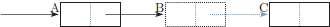
\includegraphics{figures/intro_1}
  \caption[Η πρόωρη διαγραφή ενός αντικειμένου μπορεί να οδηγήσει
           σε σφάλματα]
    {Η πρόωρη διαγραφή ενός αντικειμένου μπορεί να οδηγήσει σε
     σφάλματα. Εδώ η μνήμη του αντικειμένου B έχει ανακτηθεί. Το
     ζωντανό αντικείμενο A περιέχει πλέον έναν ξεκρέμαστο δείκτη.
     Ταυτόχρονα, υπάρχει διαρροή μνήμης: η μνήμη που καταλαμβάνει
     το αντικείμενο C δεν μπορεί να ανακτηθεί παρότι αυτό δεν
     είναι προσβάσιμο.}
   \label{fig:intro_1}  
\end{figure}

\section{Ρητή αποδέσμευση μνήμης}
Κάθε μη τετριμμένο πρόγραμμα το οποίο τρέχει με πεπερασμένη μνήμη
στη διάθεσή του, χρειάζεται κατά καιρούς να επανακτήσει τη μνήμη
που φιλοξενεί αντικείμενα μη χρήσιμα στους υπολογισμούς. Η μνήμη
που χρησιμοποιείται από αντικείμενα του σωρού μπορεί να ανακτηθεί
είτε χρησιμοποιώντας \textbf{ρητή αποδέσμευση} (όπως για παράδειγμα
συμβαίνει με τις συναρτήσεις free στη γλώσσα C ή delete στη
γλώσσα C++) είτε αυτόματα από το \textbf{σύστημα εκτέλεσης},
χρησιμοποιώντας καταμέτρηση αναφορών όπως ο Collins \cite{DBLP:journals/cacm/Collins60}
είτε έναν συλλέκτη σκουπιδιών εξιχνίασης όπως ο McCarthy
\cite{DBLP:journals/cacm/McCarthy60}. Η ρητή αποδέσμευση μνήμης
είναι ευάλωτη σε δύο είδη σφαλμάτων.

Πρώτον, η μνήμη ενός αντικειμένου μπορεί να αποδεσμευθεί πρόωρα και
ενώ υπάρχουν ακόμη αναφορές προς το αντικείμενο. Μία τέτοια αναφορά
ονομάζεται \textbf{ξεκρέμαστος δείκτης}. Το αποτέλεσμα που προκύπτει
αν ένα πρόγραμμα ακολουθήσει έναν τέτοιο δείκτη είναι απρόβλεπτο.
Ο προγραμματιστής δεν έχει κανέναν έλεγχο όσον αφορά το τι συμβαίνει
με την αποδεσμευμένη μνήμη: το σύστημα εκτέλεσης μπορεί να επιλέξει,
μεταξύ άλλων να την καθαρίσει (εγγράψει με μηδενικά), να την
εκχωρήσει για την αποθήκευση ενός νέου αντικειμένου ή να την
επιστρέψει στο λειτουργικό σύστημα. Το καλύτερο σενάριο στο οποίο
μπορεί ο προγραμματιστής να ελπίζει είναι ο βίαιος τερματισμός του
προγράμματος. Είναι ωστόσο πιθανότερο το πρόγραμμα να συνεχίσει
την εκτέλεσή του για εκατομμύρια κύκλους πριν τερματιστεί (καθιστώντας
την αποσφαλμάτωση επίπονη) ή ακόμη και να ολοκληρώσει επιτυχώς
την εκτέλεσή του παράγοντας ωστόσο λανθασμένα αποτελέσματα
(γεγονός που ανιχνεύεται δύσκολα).

Δεύτερον, ο προγραμματιστής μπορεί να αποτύχει να αποδεσμεύσει
τη μνήμη από ένα αντικείμενο το οποίο δε χρειάζεται πια το πρόγραμμα,
οδηγώντας με τον τρόπο αυτό σε \textbf{διαρροή μνήμης}. Σε μικρά
προγράμματα οι διαρροές μπορούν να αγνοηθούν, ωστόσο σε μεγάλα
προγράμματα μπορεί να προκαλέσουν μείωση της επίδοσης (καθώς
ο διαχειριστής μνήμης πασχίζει να ικανοποίησει αιτήματα εκχώρησης)
είτε σε αποτυχία εκτέλεσης (αν το πρόγραμμα ξεμείνει από μνήμη).
Συχνά μάλιστα μία εσφαλμένη αποδέσμευση μπορεί να προκαλέσει
ταυτόχρονα τόσο ένα ξεκρέμαστο δείκτη όσο και μια διαρροή.

Τα προγραμματιστικά σφάλματα του τύπου αυτού είναι συνήθη σε
περιβάλλοντα όπου δύο ή και περισσότερες διαδικασίες διατηρούν
αναφορές προς το ίδιο αντικείμενο. Η κατάσταση είναι ακόμη πιο
προβληματική σε περιβάλλοντα ταυτόχρονου προγραμματισμού όπου
δύο ή περισσότερα νήματα χειρίζονται δείκτες προς το ίδιο αντικείμενο.

Τι κάνουν λοιπόν οι προγραμματιστές σε μία γλώσσα που δεν υποστηρίζει
αυτόματη δυναμική διαχείριση μνήμης; Η ερώτηση αυτή έχει απασχολήσει
αρκετούς ερευνητές με την επικρατέστερη άποψη να ισχυρίζεται πώς
ο προγραμματιστής απαιτείται να είναι συνεπής όσον αφορά τον τρόπο
με τον οποίο χειρίζεται την \textbf{ιδιοκτησία} των αντικειμένων.
Ο Belotsky \cite{belo03} και άλλοι ερευνητές προτείνουν διαφορετικές
στρατηγικές για τη γλώσσα C++. Αρχικά, οι προγραμματιστές πρέπει
να αποφεύγουν τη δέσμευση μνήμης στο σωρό, όποτε αυτό είναι
δυνατό.Τα αντικείμενα μπορούν να δεσμεύονται στη στοίβα. Και
κατά δεύτερον οι προγραμματιστές θα πρέπει να περνούν σε και να
επιστρέφουν από συναρτήσεις/διαδικασίες αντικείμενα κατά τιμή,
αντιγράφοντας όλα τα περιεχόμενα της παραμέτρου ή του αποτελέσματος
αντί να περνούν δείκτες σε αυτά. Είναι προφανές πώς και οι δύο
προσεγγίσεις αποτρέπουν τα σφάλματα που αφορούν την εκχώρηση και
αποδέσμευση μνήμης αλλά συνοδεύονται από αυξημένη κίνηση μνήμης
και απώλεια δυνατότητας διαμοιρασμού δεδομένων. Σε μερικές περιπτώσεις
επίσης μπορούν να χρησιμοποιηθούν ειδικοί εκχωρητές, οι οποίοι
για παράδειγμα μπορούν να διαχειρίζονται μια δεξαμενή αντικειμένων.
Στο τέλος της φάσης ενός προγράμματος, ολόκληρη η δεξαμενή μπορεί
να αποδεσμεύεται. Στη γλώσσα προγραμματισμού C++ έχουν προταθεί
και υλοποιηθεί ειδικές κλάσεις αντικειμένων δεικτών με σκοπό
την καλύτερη διαχείριση μνήμης.

Η πληθώρα των διαφορετικών στρατηγικών για ασφαλή ρητή διαχείριση
μνήμης δημιουργεί ακόμη ένα πρόβλημα. Ποια προσέγγιση πρέπει
να ακολουθήσει ο προγραμματιστής αν πρέπει να διαχειριστεί με
συνέπεια την ιδιοκτησία των αντικειμένων; Αυτό είναι ιδιαίτερα
δύσκολο να απαντηθεί όταν χρησιμοποιείται κώδικας βιβλιοθήκης.
Προκύπτουν ερωτήματα σχετικά με το ποια προσέγγιση υιοθετεί ο
κώδικας της βιβλιοθήκης και αν όλες οι βιβλιοθήκες που χρησιμοποιεί
το πρόγραμμα υιοθετούν την ίδια προσέγγιση.

\section{Αυτόματη δυναμική διαχείριση μνήμης}
Η αυτόματη διαχείριση μνήμης επιλύει πολλά από τα παραπάνω προβλήματα.
Η \textbf{συλλογή σκουπιδιών} αποτρέπει την εμφάνιση ξεκρέμαστων
δεικτών: ένα αντικείμενο ελευθερώνεται μόνο όταν δεν υπάρχει
κάποιος δείκτης σε αυτό από προσβάσιμο αντικείμενο. Αντίστροφα,
όλα τα μη προσβάσιμα αντικείμενα θα ελευθερωθούν τελικώς από το
συλλέκτη. Όλες οι αποφάσεις σχετικά με την ανάκτηση μνήμης
ανατίθενται στο συλλέκτη, ο οποίος διαθέτει καθολική γνώση της
δομής των αντικειμένων στο σωρό και των νημάτων που έχουν πρόσβαση
σε αυτά.

Η διαχείριση μνήμης είναι ένα θέμα μηχανικής λογισμικού. Τα καλώς
σχεδιασμένα προγράμματα χτίζονται από ψηφίδες (modules) υψηλής
συνεκτικότητας και χαμηλής σύζευξης. Η αύξηση της συνεκτικότητας
και η μείωση της σύζευξης καθιστά ευκολότερη τη συντήρηση των
προγραμμάτων. Ιδανικά, ένας προγραμματιστής θα πρέπει να είναι
σε θέση να καταλαβαίνει τη συμπεριφορά μιας ψηφίδας μόνο από
τον κώδικα της ψηφίδας ή στη χειρότερη περίπτωση και από τον
κώδικα ενός μικρού αριθμού συγγενικών ψηφίδων. Η μείωση της
σύζευξης μεταξύ ψηφίδων πρακτικά σημαίνει πώς η συμπεριφορά
μιας ψηφίδας δεν εξαρτάται από την υλοποίηση κάποιας άλλης ψηφίδας.
Στα πλαίσια της σωστής διαχείρισης μνήμης, αυτό σημαίνει πώς
οι ψηφίδες δεν έχουν γνώση της εσωτερικής λειτουργίας των ψηφίδων
που υλοποιούν τη διαχείριση μνήμης. Η χειρωνακτική διαχείριση
μνήμης αντίθετα δε συμμορφώνεται με τις αρχές της μηχανικής
λογισμικού για ελαχιστοποίηση της επικοινωνίας μεταξύ ψηφίδων.
Το κύριο επιχείρημα υπέρ της αυτόματης διαχείρισης μνήμης δεν
είναι ότι απλοποιεί τη συγγραφή κώδικα (το οποίο ισχύει) αλλά
ότι διαζευγνύει το πρόβλημα της διαχείρισης μνήμης από διαπροσωπείες
αντί να το διασπείρει στον κώδικα. Επίσης διευκολύνει την επαναχρησιμοποίηση
κώδικα. Γι αυτούς τους λόγους η συλλογή σκουπιδιών αποτελεί, άμεσα
ή έμμεσα απαίτηση στο πρότυπο των περισσότερων σύγχρονων γλωσσών
προγραμματισμού. 

Τονίζουμε ωστόσο πώς η συλλογή σκουπιδιών δεν μπορεί να εξαλείψει
πλήρως την εμφάνιση σφαλμάτων που αφορούν τη μνήμη. Οι διαρροές
μνήμης αποτελούν ένα από πιο συχνά εμφανιζόμενα σφάλματα μνήμης.
Παρότι η συλλογή σκουπιδιών τείνει να μειώσει την εμφάνιση διαρροών
μνήμης, δεν μπορεί να εγγυηθεί την πλήρη εξάλειψή τους. Εάν ένα
αντικείμενο δεν είναι πλέον προσβάσιμο από το υπόλοιπο πρόγραμμα,
ο συλλέκτης θα ανακτήσει τη μνήμη που αυτό καταλαμβάνει. Εφόσον
αυτός είναι ο μόνος τρόπος με τον οποίο ένα αντικείμενο μπορεί
να διαγραφεί, δεν μπορούν να προκύψουν ξεκρέμαστοι δείκτες.
Επιπλέον, αν η διαγραφή ενός αντικειμένου καθιστά και τα αντικείμενα
παιδιά του μη προσβάσιμα, τότε ο συλλέκτης θα ανακτήσει και τη
μνήμη που αυτά καταλαμβάνουν. Ωστόσο, ο συλλέκτης δεν μπορεί να
βοηθήσει κάπως αν υπάρχει μια δυναμική δομή δεδομένων η οποία
συνεχώς αυξάνεται (για παράδειγμα επειδή ο προγραμματιστής εσφαλμένα
μόνο προσθέτει σε αυτή δεδομένα χωρίς ποτέ να αφαιρεί) ή αν αυτή
είναι μεν προσβάσιμη από το υπόλοιπο πρόγραμμα αλλά αυτό δε θα
τη χρησιμοποιήσει ποτέ στο μέλλον.

\section{Συκρίνοντας αλγορίθμους συλλογής σκουπιδιών}
Η παρούσα εργασία εξετάζει μια ευρεία γκάμα αλγορίθμων για συλλογή
σκουπιδιών, κάθε ένας από τους οποίους έχει σχεδιασθεί λαμβάνοντας
υπόψιν διαφορετικές απαιτήσεις όσον αφορά το φoρτίο εργασίας,
το υλικό και τις επιδόσεις. Δυστυχώς, δεν υπάρχει κάποιος αλγόριθμος
που λειτουργεί βέλτιστα σε όλες τις περιπτώσεις. Οι Fitzgerald
και Tarditi \cite{DBLP:conf/iwmm/FitzgeraldT00} μελετώντας 6 
διαφορετικούς συλλέκτες και 20 benchmarks διαπίστωσαν πώς για
κάθε συλλέκτη υπάρχει τουλάχιστον ένα benchmark το οποίο θα εκτελούταν
τουλάχιστον 15\% ταχύτερα με την παρουσία ενός πιο κατάλληλου
συλλέκτη. Ο Singer κ.ά. \cite{DBLP:conf/iwmm/SingerBWC07} εφαρμόζουν
τεχνικές μηχανικής μάθησης προκειμένου να προβλέψουν βέλτιστη
διαμόρφωση ενός συλλέκτη για ένα συγκεκριμένο πρόγραμμα. Άλλοι
ερευνητές \cite{DBLP:conf/jvm/Printezis01,DBLP:conf/iwmm/SomanKB04}
έχουν εξερευνήσει την ιδέα να επιτρέπουν στις εικονικές μηχανές
Java να αλλάζουν συλλέκτη καθώς εκτελούνται εάν πιστεύουν, με
βάση τα χαρακτηριστικά του υπό εκτέλεση προγράμματος πώς αυτό
θα ωφεληθεί από την παρουσία ενός διαφορετικού συλλέκτη. Στην
ενότητα αυτή παρουσιάζουμε τις μετρικές βάση των οποίων συγκρίνονται
οι διαφορετικοί αλγόριθμοι συλλογής σκουπιδιών. Τονίζουμε ωστόσο
πώς οι μετρικές αυτές δεν είναι ανεξάρτητες μεταβλητές: η ρύθμιση
μιας παραμέτρου με σκοπό την επίτευξη ενός συγκεκριμένου στόχου
ενδέχεται να προκαλέσει άλλες αντιφατικές επιδράσεις.

\subsection{Ασφάλεια}
Ένας αλγόριθμος συλλoγής σκουπιδιών πρέπει καταρχήν να είναι
\textbf{ασφαλής}: δεν πρέπει ποτέ να ανακτήσει τη μνήμη αντικειμένων
που είναι ζωντανά. Η εξασφάλιση της ασφάλειας είναι ιδιαίτερα
δύσκολη σε ταυτόχρονους συλλέκτες. Επίσης η ασφάλεια της
\textbf{συντηρητικής συλλογής σκουπιδιών}, όπου ο συλλέκτης δεν
έχει καμία απολύτως βοήθεια από το μεταγλωττιστή και το σύστημα
εκτέλεσης, είναι ευάλωτη σε συγκεκριμένες βελτιστοποιήσεις του
μεταγλωττιστή οι οποίες έχουν ως αποτέλεσμα δεδομένα που
δεν είναι δείκτες να φαίνεται ότι είναι.

\subsection{Ρυθμαπόδοση}
Κοινή απαίτηση των χρηστών είναι τα προγράμματά τους να τρέχουν
ταχύτερα. Για να συμβαίνει αυτό, πρέπει μεταξύ άλλων, ο υπολογιστικός
χρόνος που αφορά συλλογή σκουπιδιών να είναι ο ελάχιστος δυνατός.
Στις περισσότερες περιπτώσεις βέβαια, ο χρήστης ενδιαφέρεται το
σύνολο της εφαρμογής (τροποποιητής και συλλέκτης) να εκτελείται
σε όσο το δυνατόν λιγότερο χρόνο. Στα περισσότερα καλώς σχεδιασμένα
συστήματα, ξοδεύεται πολύ περισσότερος χρόνος CPU για την εκτέλεση
του τροποποιητή από ότι για την εκτέλεση του συλλέκτη. Έτσι πολλές
φορές αξίζει να θυσιαστεί η επίδοση του συλλέκτη χάριν υψηλότερης 
διεκπεραιωτικής ικανότητας του τροποποιητή.

\subsection{Πληρότητα και προθυμία}
Ιδανικά, η συλλογή σκουπιδιών οφείλει να είναι \textbf{πλήρης}: 
τελικώς όλα τα σκουπίδια στο σωρό θα συλλεγούν. Ωστόσο, αυτό
δεν είναι πάντοτε δυνατό ή και επιθυμητό. Όπως θα δούμε και στο
κεφάλαιο~\ref{ch:refcnt}, οι απλοϊκοί αλγόριθμοι καταμέτρησης
αναφορών για παράδειγμα αδυνατούν να συλλέξουν αυτοαναφορικές
δομές δεδομένων. Επιπλέον, για λόγους επίδοσης, μπορεί να είναι 
επιθυμητό να μη συλλεγεί ολόκληρος ο σωρός σε κάθε κύκλο συλλογής.
Οι γενεαλογικοί συλλέκτες για παράδειγμα, διαχωρίζουν τα αντικείμενα
με βάση την ηλικία τους σε δύο ή περισσότερες περιοχές του σωρού
τις οποίες ονομάζουν γενεές. Επικεντρώνοντας την προσοχή τους στη
νεότερη γενιά, οι γενεαλογικοί συλλέκτες βελτιώνουν τόσο το συνολικό
χρόνο εκτέλεσης του συλλέκτη όσο και το μέσο χρόνο παύσης του
τροποποιητή για την κάθε ξεχωριστή ενεργοποίηση αυτού. 

Οι ταυτόχρονοι συλλέκτες αναμιγνύουν την εκτέλεση τροποποιητή
και συλλέκτη με στόχο την αποφυγή ή έστω τη μείωση της χρονικής
διάρκειας των διακοπών του προγράμματος χρήστη. Μια συνέπεια
αυτού είναι πώς τα αντικείμενα που έχουν γίνει σκουπίδια αφού
έχει ξεκινήσει ένας κύκλος συλλογής μπορεί να μην ελευθερωθούν
παρά στο τέλος του επόμενου κύκλου. Τέτοια αντικείμενα ονομάζονται
\textbf{αιωρούμενα σκουπίδια}. Σε ένα περιβάλλον λοιπόν όπου
συλλέκτης και τροποποιητής εκτελούνται ταυτόχρονα η πληρότητα
του συλλέκτη σχετίζεται με την \textbf{τελική} συλλογή των σκουπιδιών. 
Διαφορετικοί αλγόριθμοι μπορεί να διαφέρουν ως προς την 
\textbf{προθυμία} συλλογής τους, οδηγώντας σε συμβιβασμούς χώρου
/χρόνου. 

\subsection{Χρόνος παύσης}
Μια σημαντική απαίτηση συνήθως είναι η ελαχιστοποίηση της εισβολής
του συλλέκτη στην εκτέλεση του προγράμματος. Πολλοί συλλέκτες
εισάγουν παύσεις στην εκτέλεση ενός προγράμματος καθώς όλα τα
νήματα του τροποποιητή είναι σταματημένα την ώρα που αυτοί συλλέγουν
σκουπίδια. Ο όρος \textbf{παύση του κόσμου} αναφέρεται ακριβώς
στην αναστολή της εκτέλεσης των νημάτων τροποποιητών κατά τη
διάρκεια της εκτέλεσης των νημάτων συλλεκτών. Είναι εμφανώς
επιθυμητό οι \textbf{χρόνοι παύσης} να ελαχιστοποιηθούν. Αυτό
μπορεί να είναι ιδιαίτερα σημαντικό για διαδραστικές εφαρμογές
ή διακομιστές οι οποίοι χειρίζονται συναλλαγές (όπου συνήθως οι
ενέργειες πρέπει να διεκπεραιώνονται εντός πολύ στενών χρονικών
ορίων). Ωστόσο, οι μηχανισμοί που προσπαθούν να μειώσουν τους
χρόνους παύσης έχουν παρενέργειες όπως θα δούμε στη συνέχεια.
Για παράδειγμα οι γενεαλογικοί συλλέκτες προσπαθούν να μειώσουν
τους χρόνους παύσης συλλέγοντας συχνά και γρήγορα μία μικρή
περιοχή του σωρού που φιλοξενεί νέα αντικείμενα ενώ συλλέγουν
μεγαλύτερες περιοχές του σωρού όπου ζουν παλαιά αντικείμενα
σπανιότερα και μόνο αν αυτό χρειασθεί. Ωστόσο, επειδή πρέπει
να καταγράφονται οι δείκτες που περνούν τα όρια των περιοχών,
η γενεαλογική συλλογή σκουπιδιών επιβάλλει ένα μικρό πρόστιμο
στις λειτουργίες εγγραφής δεικτών του τροποποιητή.

Οι παράλληλοι συλλέκτες σταματούν τα νήματα του τροποιητή και
μειώνουν το χρόνο παύσης απασχολώντας πολλά νήματα. Οι αυξητικοί
και ταυτόχρονοι συλλέκτες επιχειρούν να μειώσουν τους χρόνους
παύσης ακόμη περισσότερο εκτελώντας ένα μικρό κβάντο εργασιών
συλλογής είτε ανάμεσα στις λειτουργίες του τροποποιητή είτε
παράλληλα με αυτές. Και αυτές οι τεχνικές υπαγορεύουν ένα μικρό
κόστος στον τροποποιητή προκειμένου να επιτευχθεί ο σωστός συγχρονισμός 
αυτού με το συλλέκτη.

Η μέγιστη τιμή ή ο μέσος χρόνος παύσης ωστόσο δεν μπορούν να
χρησιμοποιηθούν ώστε να ελεγχθεί η πρόοδος του τροποποιητή. Η
κατανομή των χρόνων παύσης είναι επίσης μια μετρική που ενδιαφέρει.
Στη βιβλιογραφία συναντώνται διάφοροι τρόποι μέτρησης αυτής,
όπως η \textbf{ελάχιστη χρησιμοποίηση τροποποιητή} \cite{DBLP:conf/pldi/ChengB01},
και η \textbf{φραγμένη χρησιμοποίηση τροποποιητή} \cite{DBLP:conf/oopsla/SachindranMB04}.
Και οι δύο μετρικές προσπαθούν να μετρήσουν με ακρίβεια το
ελάχιστο κλάσμα του χρόνου εκτέλεσης που δαπανάται για την
εκτέλεση του τροποποιητή.

\subsection{Επιβάρυνση σε χώρο}
Ο στόχος ενός διαχειριστή μνήμης είναι η ασφαλής και αποδοτική
χρήση του χώρου. Διαφορετικοί διαχειριστές, τόσο ρητοί όσο και
αυτόματοι επιβάλλουν διαφορετικά \textbf{χωρικά κόστη}. Οι συλλέκτες
με καταμέτρηση αναφορών για παράδειγμα χρειάζονται χώρο στη
μνήμη κάθε αντικειμένου όπου θα αποθηκεύεται ο μετρητής αναφορών
προς αυτό. Οι συλλέκτες με σήμανση και εκκαθάριση αποθηκεύουν
ένα bit/byte στην επικεφαλίδα ενός αντικειμένου, ενώ κάποιοι
συλλέκτες με σήμανση και συμπύκνωση αποθηκεύουν τη νέα διεύθυνση
ενός αντικειμένου σε κάποιο πεδίο στο παλαιό αντίγραφο αυτού.
Οι συλλέκτες αντιγραφής διαχωρίζουν το σωρό σε δύο ημιχώρους,
μόνο ένας εκ των οποίων είναι διαθέσιμος στον τροποποιητή κάθε
χρονική στιγμή: ο άλλος χρησιμεύει ως αντίγραφο ρεζέρβα όπου
ο συλλέκτης θα αντιγράψει τα ζωντανά αντικείμενα στη διάρκεια
του επόμενου κύκλου συλλογής. Οι συλλέκτες ενδέχεται επίσης να
χρησιμοποιούν βοηθητικές δομές δεδομένων. Οι ταυτόχρονοι συλλέκτες,
ή οι γενεαλογικοί συλλέκτες απαιτούν τη χρήση ενθυμούμενων συνόλων
ώστε να καταγράφουν τις τιμές ποιων δεικτών έχει μεταβάλλει στο
ενδιάμεσο ο τροποποιητής ή τις διευθύνσεις των διαγενεαλογικών
δεικτών αντίστοιχα.

\subsection{Βελτιστοποιήσεις για ειδικές γλώσσες}
Οι αλγόριθμοι συλλογής σκουπιδιών πολλές φορές χαρακτηρίζονται
από την εφαρμοσιμότητά τους σε γλώσσες προγραμματισμού διαφορετικών
οικογενειών. Οι συναρτησιακές γλώσσες για παράδειγμα προσφέρονται
για βελτιστοποιήσεις που σχετίζονται με την αυτόματη διαχείριση
μνήμης. Μερικές γλώσσες, όπως η ML διακρίνουν τα δεδομένα σε
τροποποιήσιμα και μη τροποποιήσιμα. Αγνές συναρτησιακές γλώσσες
όπως η Haskell, επεκτείνουν την παραπάνω ιδέα και δεν αφήνουν
τον προγραμματιστή να τροποποιήσει καμία τιμή (τα προγράμματα
χαρακτηρίζονται από διαφάνεια αναφορών). Εσωτερικά ωστόσο, ενημερώνουν
δομές δεδομένων τουλάχιστον μια φορά, κάτι που δίνει τη δυνατότητα
σε γενεαλογικούς συλλέκτες σκουπιδιών να προάγουν πρόθυμα πλήρως
υπολογισμένες δομές δεδομένων. Έχουν επίσης προταθεί \textbf{πλήρεις}
μηχανισμοί για τη συλλογή κύκλων σκουπιδιών με καταμέτρηση αναφορών.
Οι δηλωτικές γλώσσες προγραμματισμού ενδεχομένως επιτρέπουν τη
χρήση μηχανισμών για αποδοτική διαχείριση του σωρού. Όλα τα δεδομένα
που έχουν δημιουργηθεί μετά από ένα σημείο επιλογής σε μία γλώσσα
λογικού προγραμματισμού καθίστανται μη προσβάσιμα τη χρονική
στιγμή κατά την οποία το πρόγραμμα οπισθοχωρεί στο εν λόγω σημείο.
Εάν ο διαχειριστής μνήμης διατάσσει τα αντικείμενα στο σωρό με
βάση τη σειρά δημιουργίας τους, η συνολική μνήμη που έχει εκχωρηθεί
από το σημείο επιλογής και έπειται μπορεί να επιστραφεί σε σταθερό
χρόνο. Αντίστροφα, διαφορετικά πρότυπα γλωσσών μπορεί να ορίζουν
συγκεκριμένες απαιτήσεις από το συλλέκτη. Οι πιο γνωστές αφορούν
την ικανότητα του συλλέκτη να χειρίζεται διάφορα είδη δεικτών
ή να προκαλεί την οριστικοποίηση (finalization) νεκρών αντικειμένων. 

\subsection{Κλιμακωσιμότητα και μεταφερσιμότητα}
Η ολοένα και περισσότερο αυξανόμενη διάδοση πολυπύρηνων επεξεργαστών
σε επιτραπέζιους και φορητούς υπολογιστές πέραν των διακομιστών
μεγάλης κλίμακας καθιστά ιδιαίτερα σημαντική την ανάγκη η συλλογή
σκουπιδιών να επωφεληθεί από την παρουσία του παράλληλου υλικού.
Έτσι συχνά ένας αλγόριθμος συλλογής σκουπιδιών χαρακτηρίζεται
ως προς το πώς \textbf{κλιμακώνει}. Η λειτουργία ενός αριθμού
αλγορίθμων συλλογής σκουπιδιών εξαρτάται από την υποστήριξη που
παρέχει το λειτουργικό σύστημα και η αρχιτεκτονική. Αυτό έχει
ως αποτέλεσμα η \textbf{μεταφερσιμότητα} των αλγορίθμων να μην
είναι απαραίτητα εγγυημένη.

\section{Ορολογία}
Στην ενότητα αυτή εξηγούμε την ορολογία που χρησιμοποιείται
στην εργασία αυτή αλλά και στη βιβλιογραφία.

Ο \textbf{σωρός} είναι είτε ένας συνεχόμενος πίνακας από λέξεις
μνήμης ή ένα σύνολο από μη συνεχόμενα μπλοκ συνεχόμενων λέξεων.
Ένα \textbf{αντικείμενο} είναι ένα σύνολο από συνεχόμενες λέξεις
μνήμης. Οι επιμέρους λέξεις ενός αντικείμενου αναφέρονται και ως
\textbf{πεδία}. Σε κάθε πεδίο ενός αντικειμένου αποθηκεύεται ένα
βαθμωτό μέγεθος (π.χ ένας ακέραιος) ή μια \textbf{αναφορά}. Μια
αναφορά είναι είτε ένας δείκτης προς ένα αντικείμενο του σωρού
είτε η ειδική τιμή \textbf{null}. Ένα αντικείμενο συνήθως έχει
ένα ειδικό πεδίο, την \textbf{επικεφαλίδα}, όπου αποθηκεύονται
μεταδεδομένα χρήσιμα για το σύστημα εκτέλεσης. Ο σωρός συχνά
αναφέρεται και ως \textbf{γράφος αντικειμένων}. Ο γράφος είναι
κατευθυνόμενος, με κόμβους τα αντικείμενα του σωρού και ακμές
τους δείκτες στα πεδία αυτών. Μια ακμή αναπαριστά μια αναφορά από
έναν κόμβο αφετηρίας ή μία \textbf{ρίζα} προς έναν κόμβο προορισμού.

\begin{figure}[H]
 \centering
 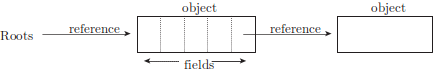
\includegraphics{figures/intro_3}
 \caption{Ρίζες, αναφορές, αντικείμενα, πεδία.}
 \label{fig:intro_3}
\end{figure}
 
Σύμφωνα με τον Dijkstra \cite{DBLP:conf/ac/DijkstraLMSS75,
DBLP:journals/cacm/DijkstraLMSS78}, ένα πρόγραμμα με συλλογή
σκουπιδιών διαχωρίζεται στα εξής δύο ημιανεξάρτητα τμήματα:

\begin{itemize}
\item Ο \textbf{τροποποιητής} εκτελεί τον κώδικα της εφαρμογής,
      ο οποίος δημιουργεί αντικείμενα και τροποποιεί το γράφο
      αντικειμένων μεταβάλλοντας αναφορές ώστε αυτές να αναφέρονται
      σε διαφορετικά αντικείμενα προορισμού. Μια αναφορά μπορεί
      να περιέχεται στο πεδίο ενός αντικειμένου ή στις ρίζες
      του πρόγράμματος (στατικές μεταβλητές, καταχωρητές, στοίβα).
      Καθώς ο τροποποιητής τροποποιεί τις αναφορές, κάθε αντικείμενο
      μπορεί να αποσυνδεθεί από τις ρίζες, δηλαδή να μην είναι
      πλέον προσβάσιμο ακολουθώντας μια ακολουθία αναφορών από
      αυτές.
\item Ο \textbf{συλλέκτης} εκτελεί κώδικα συλλογής σκουπιδιών,
      ο οποίος ανακαλύπτει μη προσβάσιμα αντικείμενα και ανακτά
      τη μνήμη που αυτά καταλαμβάνουν.
\end{itemize}

Ο τροποποιητής μπορεί να είναι είτε \textbf{μονονηματικός}
είτε \textbf{πολυνηματικός}. Το ίδιο ισχύει και για το συλλέκτη.

Εκτός από το σωρό, θεωρούμε πώς υπάρχει ένα (πεπερασμένο) σύνολο
ριζών, το οποίο αναπαριστά δείκτες που είναι \textbf{άμεσα}
προσβάσιμοι από τον τροποποιητή. Κατά επέκταση, τα αντικείμενα
του σωρού στα οποία αναφέρονται οι ρίζες ονομάζονται
\textbf{αντικείμενα ρίζες}. Καθώς ο τροποποιητής εκτελείται,
οι ρίζες και άρα και ο γράφος αντικειμένων μεταβάλλονται.

Αναφερόμαστε σε έναν κόμβο του σωρού $N$ χρησιμοποιώντας τη
διεύθυνσή του στη μνήμη (η οποία δεν αντιστοιχεί απαραίτητα
στην πρώτη λέξη του αντικειμένου αλλά ίσως σε κάποιο προκαθορισμένο
σημείο ανάμεσα στα δεδομένα και τα μεταδεδομένα του αντικειμένου).
Δοθέντος ενός αντικειμένου $N$, αναφερόμαστε στο $i$-στό πεδίο
του, στο οποίο μπορεί να αποθηκεύεται μία βαθμωτή μεταβλητή ή
ένας δείκτης, ως $N[i]$, αντιμετωπίζοντας το αντικείμενο ως
έναν πίνακα από πεδία. Συμβολίζουμε με $|N|$ το πλήθος των
πεδίων ενός αντικειμένου, ενώ η αποδιευθυνσιοδότητση ενός
μη μηδενικού δείκτη $p$ συμβολίζεται με $*p$. Επιπλέον η διεύθυνση
του $i$-στού πεδίου του αντικειμένου $N$ συμβολίζεται με
$\&N[i]$. Επομένως το σύνολο των διευθύνσεων των πεδίων δεικτών
ενός αντικειμένου $N$, συμβολιζόμενο ως $Pointers(N)$ ορίζεται
αυστηρά ως:

$Pointers(N)=\{a | a=\&N[i], \forall i: 0 \leq i < |N| \; where \; N[i] \; is \; a \; pointer\}$

Τέλος, θεωρούμε το σύνολο $Roots$ των ριζών θεωρούμε ως ένα
ψευδοαντικείμενο και αναφερόμαστε στην $i$-στή ρίζα ως $Roots[i]$.

Λέμε πώς ένα αντικείμενο είναι \textbf{ζωντανό} εάν αυτό πρόκειται
να χρησιμοποιηθεί κάποια χρονική στιγμή στο μέλλον από τον τροποποιητή.
Ένας συλλέκτης σκουπιδιών είναι ορθός αν και μόνο αν ποτέ δε
συλλέγει ζωντανά αντικείμενα. Δυστυχώς ωστόσο, η ζωντάνια είναι
μια μη-αποκρίσιμη ιδιότητα των προγραμμάτων: δεν υπάρχει κάποιος
τρόπος ώστε να απαντηθεί αν ένα τυχαίο πρόγραμμα θα χρησιμοποιήσει
ή όχι στο μέλλον ένα αντικείμενο στο σωρό. Το γεγονός πώς ένα
πρόγραμμα διαθέτει ένα δείκτη προς ένα αντικείμενο δε σημαίνει
απαραίτητα και πώς αυτό θα προσπελαστεί από το πρόγραμμα κάποια
στιγμή στο μέλλον. Προσεγγίζουμε τη ζωντάνια με την αποκρίσιμη
ιδιότητα της \textbf{προσβασιμότητα μέσω δεικτών}. Ένα αντικείμενο
$N$ είναι προσβάσιμο από ένα αντικείμενο $M$, εάν το $N$ μπορεί
να προσπελασθεί ακολουθώντας μία ακολουθία δεικτών από κάποιο
πεδίο $f$ του $M$. Επομένως, ένα αντικείμενο είναι προσβάσιμο
από τις ρίζες ενός τροποποιητή αν και μόνο αν υπάρχει μια ακολουθία
δεικτών που ξεκινάει από κάποια ρίζα και καταλήγει σε αυτό.

Πιο αυστηρά, ορίζουμε την δυαδική σχέση $\rightarrow_f$ ως εξής.
Για κάθε δύο κόμβους $M, N$, ισχύει πώς $M\rightarrow_f N$ αν
και μόνο εάν υπάρχει ένα πεδίο $f = \& M[i]$, τέτοιο ώστε
$f \in Pointers(M)$ και $*f = N$. Παρόμοια, $Roots \rightarrow_f N$
αν και μόνο αν υπάρχει ένα πεδίο $f$ τέτοιο ώστε $f \in Roots$
και $*f = N$. Λέμε πώς ο κόμβος $N$ είναι \textbf{άμεσα προσβάσιμος}
από τον κόμβο $M$, και συμβολίζουμε με $M \rightarrow N$ αν υπάρχει
κάποιο πεδίο $f$ το οποίο ανήκει στο σύνολο $Pointers(M)$ και είναι
τέτοιο ώστε $M \rightarrow_f N$. Με τη βοήθεια των παραπάνω ορισμών,
το σύνολο των προσβάσιμων αντικειμένων στο σωρό ορίζεται ως το
μεταβατικό κλείσιμο από το σύνολο $Roots$ ως προς την πράξη
$\rightarrow$, δηλαδή το ελάχιστο σύνολο:

$reachable = \{ N \in Nodes \mid (\exists r \in Roots: r \rightarrow N) \lor (\exists M \in reachable: M \rightarrow N) \}$

Ένα αντικείμενο του σωρού που είναι μη προσβάσιμο από τις ρίζες
δε θα προσπελασθεί ποτέ ξανά από έναν ορθό τροποποιητή. Αντίθετα,
ένα προσβάσιμο αντικείμενο μπορεί να προσπελασθεί κάποια στιγμή
στο μέλλον. Με τον τρόπο αυτό η ζωντάνια των αντικειμένων όσον
αφορά τη συλλογή σκουπιδιών, ορίζεται μέσω της προσβασιμότητας
μέσω δεικτών. Τα μη προσβάσιμα αντικείμενα είναι σίγουρα νεκρά
και επομένως μπορούν με ασφάλεια να ελευθερωθούν. Αντίθετα,
τα προσβάσιμα αντικείμενα μπορεί να είναι ζωντανά και επομένως
πρέπει να διατηρηθούν. Παρότι δεν είναι ακριβώς ορθό, θα χρησιμοποιούμε
τους όρους \textbf{ζωντανό} και \textbf{νεκρό} αδιακρίτως με
τους όρους \textbf{προσβάσιμο} και \textbf{μη-προσβάσιμο} αντίστοιχα. 
Τέλος, ο όρος \textbf{σκουπίδι} θα χρησιμοποιείται ως συνώνυμος
του όρου μη-προσβάσιμο.

Ο \textbf{εκχωρητής}, ο οποίος μπορεί να θεωρηθεί λειτουργικά
κάθετος ως προς το συλλέκτη, υποστηρίζει δύο λειτουργίες:
\textproc{allocate}, η οποία δεσμεύει τη μνήμη που θα καταλάβει
ένα αντικείμενο και \textproc{deallocate}, η  οποία επιστρέφει
τη μνήμη στον εκχωρητή ώστε αυτός να την επαναχρησιμοποιήσει.

Ορισμένες από τις λειτουργίες που εκτελούν τα νήματα του τροποποιητή
ενδιαφέρουν το συλλέκτη: \textproc{New}, \textproc{Read} και
\textproc{Write}. Συγκεκριμένοι διαχειριστές μνήμης μπορεί να
επεκτείνουν αυτές τις βασικές λειτουργίες και να τις μετατρέπουν
σε \textbf{φράγματα}: πράξεις που επιτρέπουν τη σύγχρονη
ή ασύγχρονη επικοινωνία με το συλλέκτη. Διακρίνουμε τα φράγματα
σε \textbf{φράγματα εγγραφής} και \textbf{φράγματα ανάγνωσης}.

\begin{algorithm}
  \caption{Λειτουργίες τροποποιητή}
  \label{alg:intro1}
  \begin{algorithmic}[1]
    \Function{New}{\null}
      \State \Return{\Call{allocate}{\null}}
    \EndFunction
    \Statex
    \Function{Read}{$src$, $i$}
      \State \Return $src[i]$
    \EndFunction
    \Statex
    \Procedure{Write}{$src$, $i$, $ref$}
      \State $src[i] \gets ref$
    \EndProcedure
  \end{algorithmic}
\end{algorithm}

Στα πλαίσια της ταυτόχρονης εκτέλεσης νημάτων τροποποιητών
και νημάτων συλλεκτών, όλοι οι αλγόριθμοι συλλογής σκουπιδιών
που εξετάζουμε απαιτούν ορισμένες ακολουθίες εντολών να
εκτελούνται \textbf{ατομικά}. Για λόγους απλοποίησης αγνοούμε
τον εκάστοτε μηχανισμό που εξασφαλίζει την ατομική εκτέλεση
τμημάτων κώδικα και απλώς σημειώνουμε τα τελευταία με τη λέξη
κλειδί \textbf{atomic}. 

\section{Οργάνωση της εργασίας}
Στο κεφάλαιο αυτό εξηγούνται οι λόγοι για τους οποίους είναι
επιθυμητή η αυτόματη διαχείριση μνήμης και ορίζονται οι
έννοιες του εκχωρητή μνήμης, του συλλέκτη σκουπιδιών και του
τροποποιητή. Επίσης παρουσιάζονται τα κριτήρια με τα οποία
μπορούν να συγκριθούν οι διαφορετικές στρατηγικές συλλογής
σκουπιδιών. Το υπόλοιπο της εργασίας οργανώνεται σε δύο μέρη.

Το πρώτο μέρος περιλαμβάνει 4 κεφάλαια στα οποία εξετάζονται
με λεπτομέρεια οι θεμελιώδεις αλγόριθμοι συλλογής σκουπιδιών.
Πιο συγκεκριμένα, το κεφάλαιο~\ref{ch:mrkswp} πραγματεύεται τη
συλλογή σκουπιδιών με σήμανση και εκκαθάριση, το κεφάλαιο~\ref{ch:mrkcmp}
τη συλλογή σκουπιδιών με σήμανση και συμπύκνωση, το κεφάλαιο~\ref{ch:cop}
τη συλλογή σκουπιδιών με αντιγραφή και τέλος το κεφάλαιο~\ref{ch:refcnt}
τη συλλογή σκουπιδιών με καταμέτρηση αναφορών.  

Το δεύτερο μέρος της εξετάζει προηγμένους αλγορίθμους συλλογής
σκουπιδιών. και αποτελείται επίσης από 4 κεφάλαια. Το κεφάλαιο~\ref{ch:gen}
πραγματεύεται λεπτομερώς τη γενεαλογική συλλογή σκουπιδιών, το
κεφάλαιο~\ref{ch:par} την παράλληλη συλλογή σκουπιδιών και το
κεφάλαιο~\ref{ch:conc} την ταυτόχρονη συλλογή σκουπιδιών. Τέλος,
στο κεφάλαιο~\ref{ch:rt} δίνεται μια σύντομη εισαγωγή στη
συλλογή σκουπιδιών πραγματικού χρόνου.

\end{greek}

\part{Θεμελιώδεις αλγόριθμοι συλλογής σκουπιδιών}
\begin{greek}
\chapter{Συλλογή σκουπιδιών με σήμανση και εκκαθάριση}\label{ch:mrkswp}

Ο ιδανικός στόχος ενός συλλέκτη σκουπιδιών είναι η ανάκτηση
του χώρου που καταλαμβάνει κάθε αντικείμενο το οποίο δεν
πρόκειται να ξαναχρησιμοποιηθεί από το πρόγραμμα. Κάθε
σύστημα αυτόματης διαχείρισης μνήμης είναι επιφορτισμένο με
τις εξής υποχρεώσεις:

\begin{enumerate}
  \item να εκχωρεί χώρο για νέα αντικείμενα,
  \item να αναγνωρίζει τα ζωντανά αντικείμενα,
  \item να ανακτά το χώρο που καταλαμβάνουν τα νεκρά αντικείμενα.
\end{enumerate}

Οι υποχρεώσεις αυτές δεν είναι ανεξάρτητες. Πιο συγκεκριμένα,
ο τρόπος ανάκτησης μνήμης επηρεάζει την εκχώρηση μνήμης. Όπως
είδαμε στο κεφάλαιο~\ref{ch:intro}, το πρόβλημα της απόφασης
κατά πόσο ένα αντικείμενο είναι πραγματικά ζωντανό είναι
μη-αποκρίσιμο. Η προσβασιμότητα μέσω δεικτών δίνει μία
υπερ-προσέγγιση του συνόλου των ζωντανών αντικειμένων. Ένα
αντικείμενο θεωρείται ζωντανό αν και μόνο αν είναι προσβάσιμο
δια μέσου μιας αλυσίδας αναφορών ξεκινώντας από ένα σύνολο
(γνωστών) ριζών. Από την άλλη πλευρά, ένα αντικείμενο θεωρείται
νεκρό και η μνήμη που αυτό καταλαμβάνει μπορεί να ανακτηθεί,
αν δεν είναι προσβάσιμο από καμία τέτοια αλυσίδα αναφορών.
Παρότι ένα ζωντανό αντικείμενο ενδέχεται να μην προσπελασθεί
ξανά, ένα νεκρό αντικείμενο είναι σίγουρα νεκρό.

\begin{algorithm}
  \caption{Σήμανση-εκκαθάριση: εκχώρηση}
  \label{alg:mrkswp_1}
  \begin{algorithmic}[1]
    \Procedure{New}{\null}
      \State $ref \gets$ \Call{allocate}{\null}
      \If{$ref = \textbf{null}$} \Comment{heap is full}
        \State \Call{collect}{\null}
        \State $ref \gets$ \Call{allocate}{\null}
        \If{$ref = \textbf{null}$}
          \Comment{heap is still full}
          \State error ``Out of memory!''
        \EndIf
      \EndIf
      \State \Return{$ref$}
    \EndProcedure
    \Statex
    \Procedure{collect}{\null}
      \State \textbf{atomic}
      \State \Call{markFromRoots}{\null}
      \State \Call{sweep}{$start$, $end$}
    \EndProcedure
  \end{algorithmic}
\end{algorithm}

Ο πρώτος αλγόριθμος που εξετάζουμε είναι αυτός της 
\textbf{συλλογής με σήμανση και εκκαθάριση} και διατυπώθηκε από
τον Collins \cite{DBLP:journals/cacm/McCarthy60}. Πρόκειται για
μια απευθείας υλοποίηση της αναδρομικής ιδιότητας της προσβασιμότητας
μέσω δεικτών. Ο αλγόριθμος εκτελείται σε δύο φάσεις: αρχικά ο
συλλέκτης διασχίζει το γράφο των αντικειμένων, εκκινώντας από
τις ρίζες (καταχωρητές, στοίβα, καθολικές μεταβλητές), δια μέσου
των οποίων το πρόγραμμα έχει άμεση πρόσβαση σε αντικείμενα
και συνεχίζει ακολουθώντας μεταβλητές δείκτες και σημαίνοντας
κάθε αντικείμενο που συναντά. Η πρώτη αυτή φάση είναι γνωστή και
ως \textbf{εξιχνίαση}. Στη δεύτερη φάση, αυτήν της \textbf{εκκαθάρισης},
ο συλλέκτης εξετάζει κάθε αντικείμενο στο σωρό: κάθε μη-σημασμένο
αντικείμενο θεωρείται σκουπίδι και η μνήμη που αυτό καταλαμβάνει
απελευθερώνεται.

Ακριβώς επειδή δεν εντοπίζει τα σκουπίδια καθεαυτά, αλλά αντίθετα 
εντοπίζει τα αντικείμενα που δεν είναι σκουπίδια και έπειτα 
συμπεραίνει πώς τα υπόλοιπα είναι σκουπίδια, ο αλγόριθμος με 
σήμανση και εκκαθάριση χαρακτηρίζεται πολλές φορές και ως
\textbf{έμμεσος}. Κάθε φορά που εκτελείται, εντοπίζει 
από την αρχή τα προσβάσιμα αντικείμενα. Αντίθετα, ένας 
\textbf{άμεσος} αλγόριθμος συλλογής αποφαίνεται κατά 
πόσο ένα αντικείμενα είναι ενεργό ή μη από το αντικείμενο καθεαυτό, 
χωρίς να είναι απαραίτητη η διάσχιση του γράφου των αντικειμένων. 
Παράδειγμα ενός άμεσου αλγορίθμου αποτελεί ο αλγόριθμος 
καταμέτρησης αναφορών.

\section{Ο αλγόριθμος}
Από την πλευρά του συλλέκτη, τα νήματα τροποποιητές εκτελούν 3 
ενδιαφέρουσες ενέργειες τις \textproc{New}, \textproc{Read} και
\textproc{Write}, τις οποίες κάθε αλγόριθμος συλλογής ορίζει
με το δικό του τρόπο. Η διαπροσωπεία του συλλέκτη με τον τροποποιητή
είναι ιδιαίτερα απλή. Αν δεν είναι δυνατή η εκχώρηση μνήμης για 
ένα αντικείμενο σε ένα νήμα, καλείται ο συλλέκτης και το αίτημα 
εκχώρησης επαναλαμβάνεται. Η παρουσία της λέξης κλειδί 
\textbf{atomic} τονίζει πώς η εκτέλεση του συλλέκτη πραγματοποιείται
με παύση του κόσμου, δηλαδή χωρίς να εκτελούνται ταυτόχρονα νήματα
τροποποιητές. Αν και πάλι το αίτημα δεν μπορεί ικανοποιηθεί, η
διαθέσιμη μνήμη στο σωρό έχει εξαντληθεί. Ενώ τις περισσότερες 
φορές αυτό αποτελεί σφάλμα εκτέλεσης, σε ορισμένες γλώσσες
προγραμματισμού η συνάρτηση \textproc{New} δύναται να εγείρει
μία εξαίρεση την οποία ο προγραμματιστής μπορεί να πιάσει και
να χειριστεί.

\begin{algorithm}
  \caption{Σήμανση-εκκαθάριση: σήμανση}
  \label{alg:mrkswp_2}
  \begin{algorithmic}[1]
    \Procedure{markFromRoots}{\null}
      \State \Call{initialize}{$worklist$}
      \ForAll{$fld \in Roots$}
        \State $ref \gets *fld$
        \If{$ref \neq \textbf{null}$ \textbf{and} \textbf{not} \Call{isMarked}{$ref$}}
          \State \Call{setMarked}{$ref$}
          \State \Call{add}{$worklist$, $ref$}
          \State \Call{mark}{\null}
        \EndIf
      \EndFor
    \EndProcedure
    \Statex
    \Procedure{initialize}{\null}
      \State $worklist \gets empty$
    \EndProcedure
    \Statex
    \Procedure{mark}{\null}
      \While{\textbf{not} \Call{isEmpty}{$worklist$}}
        \State $ref \gets$ \Call{remove}{$worklist$}
        \ForAll{$fld \in Pointers(ref)$}
          \State $child \gets *fld$
          \If{$child \neq \textbf{null}$ \textbf{and} \textbf{not} \Call{isMarked}{$child$}}
            \State \Call{setMarked}{$child$}
            \State \Call{add}{$worklist$, $child$}
          \EndIf
        \EndFor
      \EndWhile
    \EndProcedure
  \end{algorithmic}
\end{algorithm}

Πριν ξεκινήσει την εξερεύνηση του γράφου αντικειμένων, ο
συλλέκτης πρέπει να αρχικοποιήσει τη λίστα εργασιών ($worklist$) 
με τα αντικείμενα εκκίνησης της εξερεύνησης (διαδικασία
\textproc{markFromRoots}). Κάθε αντικείμενο ρίζα σημαίνεται 
και τοποθετείται στη λίστα εργασιών. Η σήμανση κωδικοποιείται 
συνήθως με την τιμή ενός bit/byte το οποίο αποθηκεύεται είτε 
στην κεφαλίδα του αντικειμένου είτε σε έναν ξεχωριστό πίνακα 
(bitmap table). Αν ένα αντικείμενο δεν περιέχει δείκτες, 
απλώς σημαίνεται και δεν εισάγεται στη λίστα εργασιών, αφού 
αυτό δεν είναι απαραίτητο καθώς δεν έχει παιδιά. Για να
ελαχιστοποιηθεί το μέγεθος της λίστας εργασιών, η 
\textproc{markFromRoots} καλεί αμέσως τη διαδικασία
\textproc{mark}. Εναλλακτικά, μπορεί να είναι επιθυμητή
η όσο το δυνατόν γρηγορότερη σάρωση των ριζών κάθε νήματος
τροποποιητή. Για παράδειγμα ένας ταυτόχρονος συλλέκτης 
μπορεί να διακόπτει την εκτέλεση ενός νήματος για πολύ
μικρό χρονικό διάστημα ώστε να σαρώσει τη στοίβα του
και να συνεχίσει με την εξερεύνηση του γράφου ενώ το
τελευταίο εκτελείται.

Η λίστα εργασιών μπορεί να υλοποιηθεί ως μία στοίβα, οδηγώντας 
έτσι σε μία κατά βάθος διάσχιση του γράφου των αντικειμένων. 
Αν μάλιστα τα bit σήμανσης βρίσκονται αποθηκευμένα μαζί με 
τα αντικείμενα (π.χ.\ στην κεφαλίδα των τελευταίων), τότε τα 
επόμενα αντικείμενα που πρόκειται να εξεταστούν, αυτά που 
είναι ήδη σημασμένα, βρίσκονται με μεγάλη πιθανότητα στην 
μνήμη cache. Η τοπικότητα των αναφορών μπορεί να επιδράσει
σε μεγάλο βαθμό την επίδοση του συλλέκτη.

Η σήμανση του γράφου των αντικειμένων υλοποιείται από έναν 
απλό βρόχο while. Ο δείκτης σε ένα αντικείμενο εξάγεται από 
τη λίστα εργασιών και οι δείκτες του αντικειμένου αυτού, 
εφόσον δε δείχνουν σε σημασμένα αντικείμενα εισάγονται σε 
αυτή, μέχρις ότου η λίστα εργασιών αδειάσει. Σε αυτήν την
εκδοχή της \textproc{mark} κάθε αντικείμενο προς το οποίο
υπάρχει αναφορά στη λίστα εργασιών είναι σημασμένο. 
Ο τερματισμός της διαδικασίας \textproc{mark}, επομένως και 
της \textproc{markFromRoots} εξασφαλίζεται από το γεγονός 
πώς ένας δείκτης σε ήδη σημασμένο αντικείμενο δεν εισάγεται 
στη λίστα εργασιών. Κατά την επιστροφή της \end{greek} \textproc{markFromRoots}, \begin{greek} 
κάθε αντικείμενο που είναι προσβάσιμο από τις ρίζες του 
προγράμματος έχει σημανθεί. Κάθε μη σημασμένο αντικείμενο 
είναι σκουπίδι και η μνήμη που αυτό καταλαμβάνει μπορεί να 
απελευθερωθεί.

\begin{algorithm}
  \caption{Σήμανση-εκκαθάριση: εκκαθάριση}
  \label{alg:mrkswp_3}
  \begin{algorithmic}[1]
    \Procedure{sweep}{$start$, $end$}
      \State $scan \gets start$
      \While{$scan < end$}
        \If{\Call{isMarked}{$scan$}}
          \State \Call{unsetMarked}{$scan$}
        \Else
          \State \Call{free}{$scan$}
        \EndIf
        \State $scan \gets$ \Call{nextObject}{$scan$}
      \EndWhile
    \EndProcedure
  \end{algorithmic}
\end{algorithm}

Η φάσης της εκκαθάρισης υλοποιείται από τη διαδικασία 
\textproc{sweep}. Σαρώνεται ο σωρός και είτε αφαιρείται η 
σήμανση από ένα σημασμένο αντικείμενο, είτε ελευθερώνεται η 
μνήμη που είχε εκχωρηθεί σε ένα μη σημασμένο αντικείμενο.
Ας παρατηρήσουμε πώς το κόστος αφαίρεσης της σήμανσης μπορεί 
να αποφευχθεί αν η σημασία των bit/byte σήμανσης εναλλάσσεται 
μεταξύ δύο διαδοχικών συλλογών.

Η συλλογή με σήμανση και εκκαθάριση επιβάλλει ορισμένους
περιορισμούς όσον αφορά την οργάνωση του σωρού. Πρώτον, δε
μετακινεί αντικείμενα. Αυτό έχει ως αποτέλεσμα ο διαχειριστής
μνήμης να πρέπει να είναι ιδιαίτερα προσεκτικός προκειμένου ο
σωρός να μην κατακερματισθεί σε τέτοιο βαθμό ώστε ο εκχωρητής
να μην μπορεί πλέον να ικανοποιεί αιτήματα, καθώς αυτό θα έχει
ως αποτέλεσμα είτε τη δραματική αύξηση της συχνότητας κλήσης
του συλλέκτη είτε, στη χειρότερη περίπτωση την παντελή 
αδυναμία εκχώρησης μνήμης. Επιπλέον, ο εκκαθαριστής πρέπει
να μπορεί να προσδιορίσει τη θέση κάθε κόμβου στο σωρό ακόμη
και υπό την παρουσία παραγεμίσματος (padding) που εισάγεται
από τις απαιτήσεις ευθυγράμμισης που έχουν οι περισσότερες
σύγχρονες αρχιτεκτονικές. Κατά συνέπεια, το έργο της 
συνάρτησης \textproc{nextObject} ενδέχεται να είναι σημαντικά
πιο πολύπλοκο από μια απλή πρόσθεση της διεύθυνσης ενός
αντικειμένου με το μέγεθος αυτού.

\section{Η τριχρωματική αφαίρεση}
Είναι ιδιαίτερα βολική η ύπαρξη ενός τρόπου περιγραφής της
κατάστασης των αντικειμένων κατά τη διάρκεια της συλλογής
(αν έχουν σημανθεί ή όχι, αν βρίσκονται στη λίστα εργασιών
κλπ). Η \textbf{τριχρωματική αφαίρεση}  είναι ένας χρήσιμος χαρακτηρισμός
των συλλεκτών εξιχνίασης ο οποίος επιτρέπει την 
επιχειρηματολογία σχετικά με την ορθότητα ενός συλλέκτη
σε όρους αναλλοίωτων την ισχύ των οποίων πρέπει αυτός να
εξασφαλίζει. 

Σύμφωνα με την τριχρωματική αφαίρεση, η συλλογή εξιχνίασης
διαιρεί το γράφο αντικειμένων σε \textbf{μαύρα} (ζωντανά) 
και \textbf{λευκά} (πιθανώς νεκρά) αντικείμενα. Αρχικά, κάθε
αντικείμενο είναι λευκό, ενώ την πρώτη φορά που ανακαλύπτεται
κατά την εξερεύνηση χρωματίζεται \textbf{γκρι}. Χρωματίζεται
δε μαύρο όταν έχει σαρωθεί και έχουν εντοπισθεί τα παιδιά του.
Διαισθητικά, ένα αντικείμενο είναι μαύρο αν ο συλλέκτης έχει
ολοκληρώσει την επεξεργασία του και γκρι αν ο συλλέκτης το
έχει ανακαλύψει αλλά δεν έχει τελειώσει ακόμη την επεξεργασία
του (ή χρειάζεται να το επεξεργασθεί ξανά). Σε αναλογία με
το χρωματισμό των αντικειμένων, ένα πεδίο δείκτης μπορεί 
επίσης να χαρακτηρισθεί ως προς το χρώμα του: γκρι όταν ο
συλλέκτης το ανακαλύπτει για πρώτη φορά και μαύρο όταν ο
συλλέκτης έχει τελειώσει την εξερεύνηση του υπογράφου που
το έχει ως ρίζα.  Η αναλογία αυτή επιτρέπει την αντιμετώπιση
των ριζών του τροποποιητή σαν αυτός να ήταν αντικείμενο
\cite{DBLP:conf/iwmm/Pirinen98}. Ένας γκρι τροποποιητής έχει
ρίζες οι οποίες δεν έχουν σαρωθεί ακόμα από το συλλέκτη. 
Ένας μαύρος τροποποιητής έχει ρίζες οι οποίες έχουν σαρωθεί
από το συλλέκτη και δε χρειάζεται να εξετασθούν ξανά. Η
εξιχνίαση προοδεύει στο σωρό με την μετακίνηση του
\textbf{μετώπου κύματος} (των γκρι αντικειμένων)
του συλλέκτη που ξεχωρίζει τα μαύρα αντικείμενα από τα
λευκά μέχρις ότου όλα τα προσβάσιμα αντικείμενα έχουν
χρωματισθεί μαύρα.

\begin{figure}[H]
  \centering
  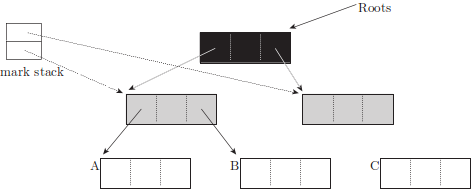
\includegraphics{figures/mrkswp_1}
  \caption[Σήμανση με τριχρωματική αφαίρεση]
    {Σήμανση με τριχρωματική αφαίρεση. Τα μαύρα αντικείμενα καθώς
     και τα παιδιά αυτών έχουν επεξεργασθεί από το συλλέκτη. Ο
     συλλέκτης γνωρίζει την ύπαρξη των γκρι αντικειμένων αλλά
     δεν έχει ολοκληρώσει την επεξεργασία τους. ο συλλέκτης δεν
     έχει επισκεφθεί ακόμη τα λευκά αντικείμενα (και μερικά δε
     τα επισκεφθεί ποτέ).}
  \label{fig:mrkswp_1}
\end{figure}

Ο αλγόριθμος της συλλογής με σήμανση και εκκαθάριση διατηρεί
μια σημαντική αναλλοίωτη: στο τέλος κάθε επανάληψης του
βρόχου σήμανσης δεν υπάρχουν αναφορές από μαύρα προς λευκά 
αντικείμενα. Επομένως κάθε λευκό προσβάσιμο αντικείμενο
είναι προσβάσιμο από κάποιο γκρι αντικείμενο. Η μη διατήρηση
της αναλλοίωτης διακινδυνεύει τη μη σήμανση ενός ζωντανού
απογόνου ενός μαύρου αντικειμένου (και κατ' επέκταση τη
λανθασμένη εκκαθάριση αυτού) καθώς ο συλλέκτης δεν 
επανεξετάζει μαύρα αντικείμενα. Η τριχρωματική αφαίρεση
είναι ιδιαίτερα χρήσιμη κατά τη θεώρηση αλγορίθμων για
ταυτόχρονη συλλογή σκουπιδιών, όπου τα νήματα τροποποιητές
εκτελούνται ταυτόχρονα με τα νήματα συλλέκτες.

\section{Σήμανση με χρήση bitmap}
Ένα bit σήμανσης συνήθως αποθηκεύεται στην επικεφαλίδα του
αντικειμένου. Εναλλακτικά, τα bits σήμανσης μπορούν να αποθηκεύονται
σε ένα ξεχωριστό bitmap στην άκρη του σωρού που συσχετίζει
κάθε ένα bit με κάθε πιθανή διεύθυνση στη μνήμη όπου μπορεί
να αποθηκευθεί ένα αντικείμενο. Ο απαιτούμενος χώρος για την
αποθήκευση του bitmap εξαρτάται από τις απαιτήσεις ευθυγράμμισης
της εικονικής μηχανής. Μπορεί να χρησιμοποιηθεί είτε ένα
καθολικό bitmap είτε αν ο σωρός είναι οργανωμένος σε μπλοκ
ένα bitmap ανά μπλοκ. Η τελευταία οργάνωση έχει ως πλεονέκτημα
πώς δεν σπαταλάται χώρος στην περίπτωση που ο σωρός δεν είναι
συνεχόμενος. Ο πίνακας bitmap για κάθε μπλοκ μπορεί να αποθηκευθεί
σε μία σταθερή θέση του μπλοκ, κάτι το οποίο ωστόσο διακινδυνεύει
την υποβάθμιση της επίδοσης, καθώς τα bitmap θα ανταγωνίζονται
για τα ίδια σύνολα σε μία συσχετιστική κρυφή μνήμη. Επιπλέον,
η πρόσβαση στο bitmap αυτόματα σημαίνει το άγγιγμα της αντίστοιχης
σελίδας. Για να αντιμετωπισθεί το πρώτο πρόβλημα, η θέση ενός
bitmap στο μπλοκ μπορεί να μεταβάλλεται και να προκύπτει για
παράδειγμα ως αποτέλεσμα της εφαρμογής μιας συνάρτησης κατακερματισμού
στη διεύθυνση του μπλοκ. Εναλλακτικά, το bitmap μπορεί να αποθηκευθεί
εκτός του μπλοκ, χρησιμοποιώντας όμως έναν πίνακα που δεικτοδοτείται
από μπλοκ (με πιθανή και πάλι χρήση κάποιας συνάρτησης κατακερματισμού).
Η τεχνική αυτή αντιμετωπίζει και τα δύο προβλήματα ταυτόχρονα.

Οι πίνακες bitmap αρκούν στην περίπτωση που η συλλογή απασχολεί
μόνο ένα νήμα σήμανσης. Διαφορετικά, η ενημέρωση ενός bit σε
έναν πίνακα bitmap είναι ευάλωτη στην απώλεια ενημερώσεων ενώ
αντίθετα η ενημέρωση ενός bit στην επικεφαλίδα ενός αντικειμένου
κινδυνεύει απλώς την εγγραφή της ίδιας τιμής εις διπλούν. Πολλοί
συλλέκτες χρησιμοποιούν πίνακες bytemap για να καταστήσουν τις
καταστάσεις συναγωνισμού ακίνδυνες. Εναλλακτικά, η τροποποίηση
ενός bit σε έναν πίνακα bitmap πρέπει να γίνεται με τη χρήση
συγχρονισμένων λειτουργιών. Στην πράξη η κατάσταση είναι επίσης
περίπλοκη όσον αφορά μεμονωμένα bits της επικεφαλίδας σε συστήματα
που επιτρέπουν ταυτόχρονη εκτέλεση συλλέκτη και τροποποιητή, καθώς
οι λέξεις της επικεφαλίδας φιλοξενούν μεταξύ άλλων και δεδομένα
τα οποία μπορεί να προσπελάσει ο τροποποιητής, όπως κλειδώματα
και κωδικοί κατακερματισμού (hash codes). Μια προσεκτική σχεδίαση
μπορεί να τοποθετήσει τα παραπάνω δεδομένα σε διαφορετικές
λέξεις της επικεφαλίδας και να εξαλείψει την ανάγκη για ατομική
τροποποίηση των bits σήμανσης αυτής.

Η χρήση bitmap σήμανσης παρουσιάζει έναν αριθμό από πλεονεκτήματα.
Ένα bitmap αποθηκεύει τα bit σήμανσης πιο πυκνά σε σύγκριση με
την αποθήκευσή τους στις επικεφαλίδες των αντικειμένων. Η χρήση
bitmap σήμανσης κατά τη συλλογή με σήμανση και εκκαθάριση συνεπάγεται
πώς η φάση της σήμανσης δεν τροποποιεί κανένα αντικείμενο, παρά
διαβάζει τα πεδία δείκτες των ζωντανών αντικειμένων. Με εξαίρεση
τη φόρτωση του πεδίου περιγραφητή τύπου, κανένα άλλο τμήμα αντικειμένων
που δεν περιέχουν δείκτες δεν προσπελάζεται Η φάση της εκκαθάρισης
δε θα διαβάσει από ούτε και θα γράψει σε κάποιο ζωντανό αντικείμενο,
παρότι μπορεί να ενημερώσει πεδία αντικειμένων σκουπιδιών στα 
πλαίσια της ανάκτησης της μνήμης που αυτά καταλαμβάνουν (για παράδειγμα
για να εισάγει ένα αντικείμενο σε μια ελεύθερη λίστα). Συνεπώς 
η σήμανση με χρήση bitmap έχει την τάση να τροποποιεί λιγότερες 
λέξεις μνήμης, με αποτέλεσμα ο αριθμός των βρώμικων μπλοκ κρυφής
μνήμης που πρέπει να αντιγραφούν στην κύρια μνήμη να μειώνεται.

Η σήμανση με τη χρήση bitmap υιοθετήθηκε αρχικά για ένα συντηρητικό
συλλέκτη που σχεδίασαν οι Boehm και Wieser \cite{DBLP:journals/spe/BoehmW88}
για την παροχή αυτόματης διαχείρισης μνήμης σε υλοποιήσεις μη 
συνεργατικών γλωσσών όπως η C και η C++. Σε συστήματα με ακριβή
πληροφορία τύπων η ταυτοποίηση κάθε θέσης μνήμης που περιέχει
ένα δείκτη είναι ακριβής ανεξάρτητα από το αν αυτή αφορά το 
εσωτερικό κάποιου αντικειμένου, τη στοίβα ή κάποια καθολική μεταβλητή.
Οι \textbf{συντηρητικοί (conservative)} συλλέκτες αντίθετα δεν
λαμβάνουν αυτό το επίπεδο υποστήριξης από το μεταγλωττιστή ή 
το σύστημα εκτέλεσης και για αυτό προβαίνουν σε συντηρητικές
αποφάσεις όσον αφορά την ταυτοποίηση δεικτών. Εάν η τιμή που
βρίσκεται σε μια θέση μνήμης μοιάζει αρκετά με δείκτη, ο συλλέκτης
αποφασίζει πώς πράγματι είναι. Είναι εμφανές πώς η συντηρητική
συλλογή σκουπιδιών ενδέχεται εσφαλμένα να διερμηνεύσει μια θέση
μνήμης ως δείκτη, κάτι που έχει δύο συνέπειες όσον αφορά την 
ασφάλεια. Πρώτον, ο συλλέκτης δεν επιτρέπεται να μεταβάλλει το
περιεχόμενο καμίας θέσης μνήμης στο χώρο διευθύνσεων του τροποποιητή
(συμπεριλαμβανομένων των ριζών). Αυτό αποκλείει αμέσως αλγορίθμους
που μετακινούν αντικείμενα, καθώς αυτό θα απαιτούσε την ενημέρωση
κάθε αναφοράς προς ένα μετακινηθέν αντικείμενο. Επίσης αποκλείει
την αποθήκευση των bits σήμανσης στις επικεφαλίδες των αντικειμένων
καθώς ένα 'αντικείμενο' για το οποίο γίνεται λόγος μπορεί να μην
είναι αντικείμενο αν η πρόσβαση σε αυτό έγινε από την εσφαλμένη
θεώρηση μιας τιμής ως δείκτη. Η τροποποίηση της τιμής ενός bit
μπορεί να καταστρέψει τα δεδομένα του χρήστη. Δεύτερον, η ελαχιστοποίηση
της πιθανότητας ο τροποποιητής να προσπελάσει δεδομένα του
συλλέκτη είναι πολύ χρήσιμη. Η προσθήκη μιας επικεφαλίδας στην
αρχή ενός αντικειμένου είναι πιο ριψοκίνδυνη από την αποθήκευση
των μεταδεδομένων του συλλέκτη όπως τα bits  σήμανσης σε μία
ξεχωριστή δομή δεδομένων.

Σύμφωνα με τον Boehm \cite{DBLP:conf/iwmm/Boehm00}, ένα επιπλέον
κίνητρο για τη σήμανση με χρήση bitmap είναι η ανάγκη για ελαχιστοποίηση 
της σελιδοποίησης που προκαλείται από τη δράση του συλλέκτη.
Στα σύγχρονα συστήματα πάντως η πρόκληση της παραμικρής σελιδοποίησης
από το συλλέκτη θεωρείται απαράδεκτη. Το ερώτημα είναι κατά πόσο
η σήμανση με χρήση bitmap μπορεί να βελτιώσει την επίδοση της
κρυφής μνήμης. Σύμφωνα με τους Hayes \cite{DBLP:conf/oopsla/Hayes91}
και Jones και Ryder \cite{DBLP:conf/iwmm/JonesR08} τα αντικείμενα
έχουν μια τάση να ζουν και να πεθαίνουν σε συστάδες. Πολλοί εκχωρητές 
προσπαθούν να τοποθετήσουν τα αντικείμενα σε γειτονικές θέσεις
μνήμης. Η εκκαθάριση με χρήση bitmap παρουσιάζει δύο πλεονεκτήματα.
Πρώτον, επιτρέπει το μαζικό έλεγχο των bits/bytes σήμανσης για 
τα αντικείμενα μιας συστάδας, καθώς είτε όλα θα έχουν τη λογική
τιμή 0 είτε όλα θα έχουν τη λογική τιμή 1. Άμεση συνέπεια του
γεγονότος αυτού είναι πώς είναι εύκολο να προσδιορισθεί από το
bitmap το κατά πόσο ένα μπλοκ μνήμης αποτελείται μόνο από
σκουπίδια και άρα μπορεί να επιστραφεί ολόκληρο στον εκχωρητή.

Ο Garner κ.ά. \cite{DBLP:conf/iwmm/GarnerBF07} χρησιμοποιούν μια
υβριδική προσέγγιση, συσχετίζοντας κάθε μπλοκ των ξεχωριστών 
ελεύθερων λιστών από μπλοκ διαφορετικού μεγέθους με ένα byte
και ταυτόχρονα αποθηκεύοντας ένα bit στην επικεφαλίδα κάθε
αντικειμένου. Το byte έχει την τιμή 0xFF αν και μόνο αν το
αντίστοιχο μπλοκ έχει ένα τουλάχιστον ζωντανό αντικείμενο.
Με τον τρόπο αυτό το byte-map επιτρέπει στον εκκαθαριστή να
εντοπίζει εύκολα τα μπλοκ που δεν έχουν κανένα ζωντανό αντικείμενο
και στη συνέχεια να τα ανακυκλώνει ολόκληρα. Το βασικό πλεονέκτημα
της προσέγγισης αυτής είναι πώς τόσο το bit στην επικεφαλίδα ενός 
αντικειμένου όσο και το αντίστοιχο byte του byte-map που αφορά
το μπλοκ στο οποίο αυτό ζει μπορούν να εγγράφονται χωρίς τη
χρήση συγχρονισμένων λειτουργιών.

\begin{algorithm}[H]
  \caption{Σήμανση με bitmap (Printezis \& Detlefs)}
  \label{alg:ms_4}
  \begin{algorithmic}[1]
    \Procedure{mark}{\null}
      \State $cur \gets$ \Call{nextInBitmap}{\null}
      \While{$cur < HeapEnd$}
        \State \Call{add}{$worklist$, $cur$}
        \State \Call{markStep}{$cur$}
        \State $cur \gets$ \Call{nextInBitmap}{\null}
      \EndWhile
    \EndProcedure
    \Statex
    \Procedure{markStep}{$start$}
      \While{\textbf{not} \Call{isEmpty}{$worklist$}}
        \State $ref \gets$ \Call{remove}{$worklist$}
        \ForAll{$fld \in Pointers(ref)$}
          \State $child \gets *fld$
          \If{$child \neq \textbf{null}$ \textbf{and} \textbf{not} \Call{isMarked}{$child$}}
            \State $\Call{setMarked}{child}$
            \If{$child < start$}
              \State \Call{add}{$worklist$, $child$}
            \EndIf
          \EndIf
        \EndFor
      \EndWhile
    \EndProcedure
  \end{algorithmic}
\end{algorithm}

Οι Printezis και Detlefs \cite{DBLP:conf/iwmm/PrintezisD00}
χρησιμοποιούν bitmap για να μειώσουν τον απαιτούμενο χώρο
για τις στοίβες σήμανσης σε έναν σχεδόν-ταυτόχρονο, γενεαλογικό
συλλέκτη. Αρχικά, ως συνήθως οι ρίζες του τροποποιητή σημαίνονται
με την εγγραφή της λογικής τιμής ορισμένων bits στο bitmap.
Στη συνέχεια, το νήμα σήμανσης σαρώνει γραμμικά το bitmap αναζητώντας
για ζωντανά αντικείμενα. Ο αλγόριθμος \ref{alg:bitmap-marking}
διατηρεί την ακόλουθη αναλλοίωτη: τα σημασμένα αντικείμενα
που βρίσκονται σε χαμηλότερες διευθύνσεις από την τιμή του
δείκτη $cur$ στη διαδικασία \textproc{mark} είναι μαύρα,
ενώ τα αντικείμενα που βρίσκονται σε υψηλότερες διευθύνσεις
είναι γκρι. Όταν εντοπίζεται το επόμενο ζωντανό (σημασμένο)
αντικείμενο, αυτό ωθείται στη στοίβα και ο έλεγχος περνά
στη διαδικασία \textproc{markStep}. Η τελευταία εκτελεί έναν
βρόχο while προκειμένου να αποκαταστήσει την αναλλοίωτη:
αντικείμενα εξωθούνται από τη στοίβα και τα παιδιά τους
σημαίνονται αναδρομικά μέχρις ότου αυτή εκκενωθεί. Αν ένα
αντικείμενο βρίσκεται σε χαμηλότερη διεύθυνση μνήμης από
την τρέχουσα τιμή του δείκτη $cur$, αυτό εισάγεται στη στοίβα
σήμανσης, αλλιώς η επεξεργασία του αναβάλλεται για αργότερα. 
Η βασική διαφορά αυτού του αλγορίθμου και του αλγορίθμου 
\ref{alg:marking} είναι αφορά στην εισαγωγή των παιδιών ενός 
αντικειμένου στη στοίβα σήμανσης. Τα αντικείμενα σημαίνονται 
αναδρομικά μόνο αν αυτά βρίσκονται πίσω από το μαύρο μέτωπο κύματος 
που κινείται γραμμικά στο σωρό. Παρότι η πολυπλοκότητα του αλγορίθμου 
αυτού είναι γραμμική ως προς το μέγεθος του χώρου που συλλέγεται, 
στην πράξη η αναζήτηση σε ένα bitmap είναι φθηνή.
 
\section{Οκνηρή εκκαθάριση}
Η χρονική πολυπλοκότητα της σήμανσης είναι $O(L)$, όπου $L$ το 
συνολικό μέγεθος των ζωντανών αντικειμένων του σωρού, ενώ η 
χρονική πολυπλοκότητα της εκκαθάρισης $O(H)$, όπου $H$ το μέγεθος 
του σωρού. Καθώς $H>L$, εκ πρώτης όψεως φαίνεται πώς το κόστος 
της εκκαθάρισης κυριαρχεί στο κόστος του αλγορίθμου συλλογής με 
σήμανση και εκκαθάριση, κάτι που στην πράξη δεν παρατηρείται. To 
``κυνήγι'' δεικτών στη φάση της σήμανσης οδηγεί σε τελείως μη 
προβλέψιμα μοτίβα πρόσβασης στη μνήμη, ενώ αντίθετα η συμπεριφορά 
της εκκαθάρισης είναι πολύ πιο προβλέψιμη. Επιπροσθέτως, το 
κόστος της εκκαθάρισης ενός αντικειμένου είναι πολύ μικρότερο από 
το κόστος της εξερεύνησης του υπογράφου των αντικειμένων με ρίζα 
αυτό. Η προφόρτωση (prefetching) αντικειμένων αποτελεί έναν τρόπο 
βελτίωσης της συμπεριφοράς της εκκαθάρισης όσον αφορά τη μνήμη 
cache. Για να αποφύγουν τον κατακερματισμό της μνήμης οι εκχωρητές 
πολλών διαχειριστών μνήμης που υποστηρίζουν συλλέκτες με σήμανση 
και εκκαθάριση τοποθετούν αντικείμενα του ίδιου μεγέθους σε 
συνεχόμενες διευθύνσεις μνήμης, οδηγώντας με τον τρόπο αυτό σε
σταθερό βήμα μοτίβου πρόσβασης μνήμης κατά την εκκαθάριση μπλοκ
από αντικείμενα του ίδιου μεγέθους. Αυτή η προσέγγιση δεν 
επιτρέπει μόνο προφόρτωση λογισμικού αλλά είναι ιδανική και για
τους μηχανισμούς προφόρτωσης υλικού που διαθέτουν οι σύγχρονοι
επεξεργαστές.

Μπορούν οι χρόνοι παύσης των νημάτων τροποποιητών για την εκτέλεση 
της φάσης της εκκαθάρισης να ελαττωθούν ή και να εξαλειφθούν 
πλήρως; Παρατηρούμε δύο ιδιότητες των αντικειμένων και των bit
σήμανσης αυτών. Πρώτον, από τη στιγμή που ένα αντικείμενο γίνεται
σκουπίδι, παραμένει σκουπίδι: δεν μπορεί να προσπελασθεί ή να
αναστηθεί από κάποιο νήμα τροποποιητή. Δεύτερον, τα νήματα
τροποποιητές δεν έχουν πρόσβαση στα bit σήμανσης. Επομένως η
εκκαθάριση μπορεί να ανατεθεί σε ξεχωριστά νήματα, τα οποία 
εκτελούνται ταυτόχρονα με τα νήματα τροποποιητές. Μια απλούστερη
λύση είναι η \textbf{οκνηρή εκκαθάριση}, HUGHES.
Η τεχνική ουσιαστικά πληρώνει το κόστος της εκκαθάρισης σε δόσεις 
με την εκκαθάριση να πραγματοποιείται από τον εκχωρητή. Στην 
απλούστερη εκδοχή η συνάρτηση \textproc{allocate} αυξάνει τον
δείκτη εκκαθάρισης μέχρις ότου βρει επαρκή χώρο σε μια ακολουθία
μη σημασμένων αντικειμένων. Ωστόσο, η εκκαθάριση ενός μπλοκ κάθε 
φορά με πολλά αντικείμενα είναι πιο αποδοτική. 

Ο αλγόριθμος \ref{alg:mrkswp5} επενεργεί σε ένα μπλοκ κάθε 
φορά. Είναι σύνηθες οι εκχωρητές να τοποθετούν στο ίδιο μπλοκ
ισομεγέθη αντικείμενα. Κάθε κλάση μεγέθους έχει ένα ή και 
περισσότερα μπλοκ εκχώρησης μνήμης καθώς και μία λίστα ανάκτησης
($reclaimList$) από μπλοκ που δεν έχουν ακόμη εκκαθαρισθεί.
Ως συνήθως ο συλλέκτης σημαίνει όλα τα ζωντανά αντικείμενα στο 
σωρό αλλά αντί να εκκαθαρίσει πρόθυμα ολόκληρο το σωρό, αυτός
επιστρέφει τα τελείως άδεια από ζωντανά αντικείμενα μπλοκ στον
εκχωρητή. Τα υπόλοιπα μπλοκ προστίθενται στην κατάλληλη λίστα
ανάκτησης με βάση το μέγεθος των αντικειμένων που φιλοξενούν.
Με τη λήξη της φάσης διακοπής του κόσμου τα νήματα τροποποιητές
επανεκκινούνται. Η συνάρτηση \textproc{allocate} αρχικά επιχειρεί
την απόκτηση μιας ελεύθερης θέσης από την αντίστοιχη κλάση 
μεγέθους. Αν η προσπάθεια αποτύχει, καλείται ο οκνηρός εκκαθαριστής
ο οποίος εκκαθαρίζει ένα ή περισσότερα εναπομείναντα μπλοκ της
αντίστοιχης λίστας $reclaimList$ μέχρις ότου το αίτημα μπορεί
να ικανοποιηθεί. Τι συμβαίνει στην περίπτωση όπου η λίστα των
όχι ακόμη εκκαθαρισμένων μπλοκ είναι κενή ή δεν υπάρχει ελεύθερη
θέση σε κανένα από τα εκκαθαρισμένα μπλοκ; Η απάντηση είναι πώς
ο εκκαθαριστής προσπαθεί να αποκτήσει ένα ολόκληρο ελεύθερο μπλοκ
από έναν κατώτερου επιπέδου εκχωρητή μπλοκ. Το φρέσκο μπλοκ
στη συνέχεια αρχικοποιείται με ρύθμιση των μεταδεδομένων αυτού
(όπως για παράδειγμα με τη δημιουργία ενός πίνακα με byte σήμανσης).
Αν πάλι δεν υπάρχουν διαθέσιμα φρέσκα μπλοκ, απαιτείται η κλήση
του συλλέκτη.

Υπάρχει ένα λεπτό ζήτημα όσον αφορά την οκνηρή εκκαθάριση σε
έναν οργανωμένο κατά μπλοκ σωρό. Ο Hughes [1982] δουλεύει με 
έναν συνεχόμενο σωρό και επομένως εξασφαλίζει πώς ο εκχωρητής θα
εκκαθαρίσει κάθε αντικείμενο πριν ξεμείνει από χώρο και καλέσει
το συλλέκτη. Ωστόσο, η οκνηρή εκκαθάριση ξεχωριστών κλάσεων
ως προς το μέγεθος δεν μπορεί να το εξασφαλίσει καθώς είναι σχεδόν
σίγουρο πώς ο εκκαθαριστής θα εξαντλήσει μια κλάση μεγέθους (και
όλα τα άδεια μπλοκ αυτής) πριν προχωρήσει στην εκκαθάριση μπλοκ
που ανήκουν σε διαφορετικές κλάσεις μεγέθους. Το γεγονός αυτό
οδηγεί σε δύο προβλήματα. Πρώτον, αντικείμενα σκουπίδια σε μη
εκκαθαρισμένα μπλοκ δεν αποδεσμεύονται, οδηγώντας σε διαρροή 
μνήμης. Αν το μπλοκ περιλαμβάνει ένα ζωντανό αντικείμενο, η 
παραπάνω διαρροή είναι αβλαβής καθώς τα αντικείμενα του μπλοκ 
δε θα ανακυκλωθούν ούτως ή άλλως πριν ο συλλέκτης πραγματοποιήσει
ένα αίτημα για αντικείμενο της κλάσης μεγέθους στην οποία ανήκει
το μπλοκ. Δεύτερον, αν όλα τα αντικείμενα σε ένα μπλοκ διαδοχικά
μετατραπούν σε σκουπίδια, έχει χαθεί η δυνατότητα ανάκτησης όλου
του μπλοκ μονομιάς.

Η απλούστερη λύση είναι η ολοκλήρωση της εκκαθάρισης όλων των
μπλοκ του σωρού πριν την έναρξη της σήμανσης. Ωστόσο, μπορεί
να είναι προτιμότερο να δοθούν σε ένα μπλοκ περισσότερες ευκαιρίες
οκνηρής εκκαθάρισής του. Ο Garner κ.ά. \cite{DBLP:conf/iwmm/GarnerBF07}
πληρώνουν ένα μικρό ποσό διαρροής για να αποφύγουν το κόστος
της πρόθυμης εκκαθάρισης στο σύστημα Jikes RVM/MMTk των Blackburn
κ.ά. \cite{DBLP:conf/iwmm/BlackburnH04}. Πιο συγκεκριμένα, αντί
ενός bit, χρησιμοποιούν ένα φραγμένο ακέραιο για τη σήμανση των
αντικειμένων. Αυτό συνήθως δεν επιφέρει επιπλέον κόστος σε χώρο
καθώς υπάρχει χώρος παραπάνω από ένα bit αν οι σημάνσεις αποθηκεύονται
στις επικεφαλίδες των αντικειμένων και συχνά ξεχωριστές δομές
σήμανσης χρησιμοποιούν byte αντί για bit. Κάθε κύκλος συλλογής
αυξάνει την τιμή σήμανσης κατά $2^K$, όπου $K$ το μέγεθος της
λέξης σήμανσης σε bits, με την τιμή σήμανσης να επανέρχεται
προφανώς στο $0$ σε περίπτωση υπερχείλισης. Με τον τρόπο αυτό,
ο συλλέκτης μπορεί να ξεχωρίσει ένα αντικείμενο που έχει σημανθεί
στον τρέχοντα κύκλο συλλογής από ένα αντικείμενο που είχε
σημανθεί σε κάποιον προηγούμενο κύκλο συλλογής. Μόνο τα αντικείμενα
με την τρέχουσα τιμή σήμανσης θεωρούνται σημασμένα. Η μηδενική
τιμή σήμανσης είναι ασφαλής καθώς, ακριβώς πριν την εμφάνισή
της, κάθε ζωντανό αντικείμενο στο σωρό είναι είτε μη σημασμένο
(η μνήμη του εκχωρήθηκε μετά τον προηγούμενο κύκλο συλλογής),
είτε έχει τη μέγιστη τιμή σήμανσης. Κάθε αντικείμενο που είναι
σημασμένο με την επόμενη τιμή σήμανσης πρέπει να έχει σημανθεί
κάποιο πολλαπλάσιο του $2^K$ αριθμό συλλογών πριν: επομένως
είναι αιωρούμενο σκουπίδι και δε σημαίνεται από το νήμα σήμανσης.
Η πιθανή προκύπτουσα διαρροή αντιμετωπίζεται σε ένα βαθμό
με τη σήμανση ολόκληρων μπλοκ. Οποτεδήποτε ο MMTk συλλέκτης
σημαίνει ένα αντικείμενο, σημαίνει επίσης και το αντίστοιχο
μπλοκ. Αν κανένα από τα αντικείμενα ενός μπλοκ δεν είναι
σημασμένο με την τρέχουσα τιμή σήμανσης, τότε ούτε και το
μπλοκ είναι και συνεπώς μπορεί να ανακτηθεί ολόκληρο, όπως
στον αλγόριθμο~\ref{alg:mrkswp5}. Λαμβάνοντας υπόψη την τάση
των αντικειμένων να ζουν και να πεθαίνουν σε συστάδες,
αναμένει κανείς πώς η παραπάνω τεχνική είναι αποδοτική.

Η οκνηρή εκκαθάριση προσφέρει έναν αριθμό από πλεονεκτήματα.
Αρχικά έχει καλή τοπικότητα: μία θέση μνήμης ενός πρώην σκουπιδιού 
τείνει να χρησιμοποιηθεί σύντομα μετά την εκκαθάριση του τελευταίου.
Επιπλέον, η αλγοριθμική πολυπλοκότητα της συλλογής με σήμανση και
εκκαθάριση είναι πλέον γραμμική ως προς το μέγεθος των ζωντανών
αντικειμένων του σωρού, ίδια με την πολυπλοκότητα της συλλογής με
αντιγραφή που εξετάζουμε στο κεφάλαιο \ref{ch:copy}. Συγκεκριμένα,
ο Boehm \cite{boehm1995dynamic} επισημαίνει πώς η συλλογή με σήμανση και οκνηρή
εκκαθάριση παρουσιάζει βέλτιστες επιδόσεις στις ίδιες συνθήκες με
τη συλλογή με αντιγραφή: όταν το μεγαλύτερο μέρος του σωρού είναι
άδειο, καθώς η αναζήτηση μη σημασμένων αντικειμένων από την οκνηρή
εκκαθάριση θα ολοκληρωθεί γρήγορα.

\begin{algorithm}
  \caption{Οκνηρή εκκαθάριση σε οργανωμένο κατά μπλοκ σωρό}
  \label{alg:mrkswp5}
  \begin{algorithmic}[1]
    \Procedure{collect}{\null}
      \State \textbf{atomic}
      \State \Call{markFromRoots}{\null}
      \ForAll{$block \; \textbf{in} \; blocks$}
        \If{\textbf{not} \Call{isMarked}{$block$}} \Comment{no objects marked in this block?}
          \State \Call{add}{$blockAllocator$, $block$} \Comment{return block to block allocator}
        \Else
          \State \Call{add}{$reclaimList$, $block$}
        \EndIf
      \EndFor
    \EndProcedure
    \Statex
    \Function{allocate}{$sz$}
      \State \textbf{atomic}
      \State $result \gets$ \Call{remove}{$sz$} \Comment{allocate from size class for sz}
      \If{$result = \textbf{null}$} \Comment{if no free slots for this size...}
        \State \Call{lazySweep}{$sz$} \Comment{sweep a little}
        \State $result \gets$ \Call{remove}{$sz$}
      \EndIf
      \State \Return{$result$} \Comment{if still null, collect}
    \EndFunction
    \Statex
    \Procedure{lazySweep}{$sz$}
      \Repeat
        \State $block \gets$ \Call{nextBlock}{$reclaimList$, $sz$}
        \If{$block \neq \textbf{null}$}
          \State \Call{sweep}{$start(block)$, $end(block)$}
          \If{\Call{spaceFound}{$block$}}
            \State \Return{\null}
          \EndIf
        \EndIf
      \Until{$block = \textbf{null}$} \Comment{reclaim list for this size class is empty}
      \State \Call{allowSlow}{$sz$}
    \EndProcedure
    \Statex
    \Procedure{allocSlow}{$sz$} \Comment{allocation slow path}
      \State $block \gets$ \Call{allocateBlock}{\null}
      \If{$block \neq \textbf{null}$} \Comment{from the block allocator}
        \State \Call{initialize}{$block$, $sz$}
      \EndIf
    \EndProcedure
  \end{algorithmic}
\end{algorithm}


\section{Ανακεφαλαίωση και θέματα προς εξέταση}
Παρά το γεγονός πώς είναι ο παλαιότερος αλγόριθμος συλλογής
σκουπιδιών, [McCarthy 1960] υπάρχουν διάφοροι λόγοι για τους 
οποίους η συλλογή με σήμανση και εκκαθάριση παραμένει ακόμα και
σήμερα ελκυστική επιλογή.

\subsection{Επιβάρυνση τροποποιητή}
Η απλούστερη εκδοχή του αλγορίθμου δεν επιβάλλει καμία επιβάρυνση
στις λειτουργίες \textproc{Read} και \textproc{Write} του 
τροποποιητή, σε αντίθεση για παράδειγμα με τη συλλογή με καταμέτρηση
αναφορών που εξετάζουμε στο κεφάλαιο \ref{ch:refcnt}.
Ωστόσο η συλλογή με σήμανση και εκκαθάριση συχνά χρησιμοποιείται
ως βασικός αλγόριθμος σε πιο εξεζητημένους συλλέκτες που απαιτούν
κάποιας μορφής συγχρονισμό μεταξύ συλλέκτη και τροποποιητή. Τόσο
οι γενεαλογικοί συλλέκτες (κεφάλαιο \ref{ch:gen}) όσο και
οι ταυτόχρονοι και αυξητικοί συλλέκτες (κεφάλαιο \ref{ch:conc})
απαιτούν από τον τροποποιητή να ενημερώνει το συλλέκτη οποτεδήποτε
τροποποιεί δείκτες.

\subsection{Ρυθμαπόδοση}
Σε συνδυασμό με την οκνηρή εκκαθάριση, η συλλογή με σήμανση και
εκκαθάριση προσφέρει υψηλή ρυθμαπόδοση. Η φάση της σήμανσης είναι
σχετικά φθηνή και κυριαρχείται από την καταδίωξη δεικτών. Χρειάζεται
απλώς να θέσει ένα bit/byte για κάθε ζωντανό αντικείμενο που
ανακαλύπτει, σε αντίθεση με τη συλλογή με αντιγραφή (κεφάλαιο
\ref{ch:copy}) ή με σήμανση και συμπύκνωση (κεφάλαιο \ref{ch:mrkcmp}) 
που αντιγράφουν ή μετακινούν αντικείμενα. Από την άλλη πλευρά, 
όπως και οι περισσότεροι συλλέκτες εξιχνίασης που εξετάζουμε
στα πρώτα κεφάλαια αυτής της εργασίας η συλλογή με σήμανση και
εκκαθάριση απαιτεί την διακοπή της εκτέλεσης των νημάτων τροποποιητών
κατά τη διάρκεια εκτέλεσης του συλλέκτη. Ο χρόνος παύσης ενός
κύκλου συλλογής εξαρτάται πρωτίστως από το πρόγραμμα που εκτελεί
ο τροποποιητής και την είσοδο αυτού και μπορεί εύκολα σε μερικές
περιπτώσεις να φθάσει και μερικά δευτερόλεπτα.

\subsection{Απαιτήσεις σε χώρο}
Η συλλογή με σήμανση και εκκαθάριση έχει σαφώς καλύτερη διαχείριση
χώρου από τη συλλογή με αντιγραφή. Ενδεχομένως να έχει καλύτερη
διαχείριση χώρου και από τη συλλογή με καταμέτρηση αναφορών. Τα
bits σήμανσης συχνά αποθηκεύονται χωρίς κόστος στις επικεφαλίδες
των αντικειμένων. Εναλλακτικά, αν χρησιμοποιείται ένας πίνακας
bitmap η επιβάρυνση σε χώρο εξαρτάται από τις απαιτήσεις ευθυγράμμισης
της αρχιτεκτονικής. Η συλλογή με καταμέτρηση αναφορών από την
άλλη πλευρά απαιτεί τη χρήση μίας λέξης μνήμης σε κάθε επικεφαλίδα
αντικειμένου για την αποθήκευση του μετρητή αναφορών του τελευταίου.
Η συλλογή με αντιγραφή έχει ακόμη χειρότερη διαχείριση του χώρου
αφού διαχωρίζει το σωρό σε δύο ισομεγέθεις ημιχώρους εκ των οποίων
μόνο ο ένας είναι ανά πάσα στιγμή διαθέσιμος στον τροποποιητή.
Από την άλλη πλευρά, οι συλλέκτες που δεν συμπυκνώνουν το σωρό,
όπως η συλλογή με σήμανση και εκκαθάριση αλλά και η συλλογή με
καταμέτρηση αναφορών απαιτούν από το διαχειριστή μνήμης τη χρήση
πιο περίπλοκων εκχωρητών. Οι επιπλέον δομές δεδομένων που απαιτούνται
για την υποστήριξη τέτοιων συλλεκτών προσθέτουν μια μη αμελητέα
επιβάρυνση. Επιπρόσθετα η συλλογή χωρίς συμπύκνωση συχνά συνοδεύεται
από κατακερματισμό της μνήμης.

Ο αλγόριθμος συλλογής σκουπιδιών με σήμανση και εκκαθάριση είναι
όπως εξηγήσαμε ένας αλγόριθμος εξιχνίασης. Ως τέτοιος, οφείλει 
να αναγνωρίσει πρώτα όλα τα ζωντανά αντικείμενα του σωρού πριν
ανακτήσει τη μνήμη που χρησιμοποιείται από νεκρά αντικείμενα. 
Η διαδικασία αυτή είναι ακριβή και θα πρέπει να εκτελείται όσο 
πιο σπάνια γίνεται. Αυτό σημαίνει πώς πρέπει να αφιερωθεί ειδικός 
χώρος στο σωρό για τη λειτουργία των συλλεκτών εξιχνίασης. Αν 
τα ζωντανά αντικείμενα καταλαμβάνουν ένα μεγάλο μέρος του σωρού 
και οι εκχωρητές εκχωρούν πολύ συχνά μνήμη ο συλλέκτης με σήμανση 
και εκκαθάριση θα καλείται πολύ συχνά. O Jones [1996] επισημαίνει 
πώς για σωρούς μεσαίου και μεγάλου μεγέθους το ποσοστό του σωρού 
που αφιερώνεται στον ειδικό χώρο για τις λειτουργίες του συλλέκτη 
μπορεί να κυμαίνεται από 20\% έως και 50\%. Οι Hertz και Berger
[2005] \cite{DBLP:conf/oopsla/HertzB05} πάντως δείχνουν πώς
η αυτόματη διαχείριση μνήμης προγραμμάτων στη γλώσσα Java με
τη χρήση συλλογής με σήμανση και εκκαθάριση ενδέχεται να απαιτήσει
έναν σωρό ακόμη και μερικές φορές μεγαλύτερο σε μέγεθος προκειμένου
να πετύχει την ίδια ρυθμαπόδοση με την χειρωνακτική διαχείριση
μνήμης αυτών με ρητή αποδέσμευση.

\subsection{Μετακίνηση ή όχι;}
Η μη μετακίνηση αντικειμένων παρουσιάζει πλεονεκτήματα και
μειονεκτήματα. Το βασικό πλεονέκτημα που προκύπτει από τη μη
μετακίνηση αντικειμένων είναι πώς καθιστά τη συλλογή με σήμανση
και εκκαθάριση κατάλληλη για χρήση σε περιβάλλοντα όπου δεν 
υπάρχει συνεργασία μεταξύ μεταγλωττιστή της γλώσσας και συλλέκτη
σκουπιδιών. Χωρίς έγκυρη πληροφορία τύπων, οι ρίζες του τροποποιητή
και πεδία δείκτες αντικειμένων δεν γίνεται να ενημερωθούν με 
νέες διευθύνσεις μετακινηθέντων αντικειμένων. Αυτό συμβαίνει 
λόγω της έλλειψης βεβαιότητας σχετικά με το αν μια μεταβλητή 
ή ένα πεδίο στο εσωτερικό ενός αντικείμενου είναι δείκτης. 

Η ασφάλεια σε μη συνεργατικά συστήματα που διαχειρίζονται από
έναν συντηρητικό συλλέκτη αποτρέπει τον τελευταίο από την
τροποποίηση δεδομένων του χρήστη (συμπεριλαμβανομένων των
επικεφαλίδων αντικειμένων). Επιπλέον ενθαρρύνει την ξεχωριστή
αποθήκευση των μεταδεδομένων του συλλέκτη από τα μεταδεδομένα
του χρήστη και του συστήματος εκτέλεσης ώστε να μειωθεί η
πιθανότητα τροποποίησης των πρώτων από τον τροποποιητή. Για 
τους παραπάνω λόγους είναι επιθυμητή η αποθήκευση των bit/byte
σήμανσης σε πίνακες bitmap και όχι στις επικεφαλίδες των
αντικειμένων.

Το πρόβλημα με τη μετακίνηση αντικειμένων είναι πώς σε εφαρμογές
που τρέχουν για πολλή ώρα, ο σωρός τείνει να κατακερματίζεται.
Ο Robson \cite{DBLP:journals/jacm/Robson71, DBLP:journals/jacm/Robson74}
αποδεικνύει πώς οι εκχωρητές σε συστήματα διαχείρισης μνήμης που
χρησιμοποιούν μη μετακινούντα συλλέκτη απαιτούν $O(\log{\frac{max}{min}})$
περισσότερο χώρο από τον ελάχιστο δυνατό, όπου $min$ και $max$
το ελάχιστο και μέγιστο δυνατό μέγεθος αντικειμένων αντίστοιχα.
Συνεπώς ένας συλλέκτης δε συμπυκνώνει το σωρό με μεγάλη πιθανότητα
καλείται συχνότερα από έναν που το συμπυκνώνει. Ακόμη, όπως
σημειώθηκε πιο πάνω, ένα ποσοστό από 20\% έως και 50\% του σωρού
πρέπει να αφιερώνεται αποκλειστικά στη λειτουργία ενός συλλέκτη
εξιχνίασης ώστε να αποφευχθεί η αυξημένη συχνότητα κλήσης του
τελευταίου.

Για να ελαχιστοποιηθεί η μείωση της επίδοσης λόγω του κατακερματισμού,
πολλές εμπορικές υλοποιήσεις συλλεκτών οι οποίες διαχειρίζονται
μια περιοχή του σωρού με σήμανση και εκκαθάριση περιοδικά χρησιμοποιούν
και διαφορετικό αλγόριθμο όπως αυτόν με σήμανση και συμπύκνωση για
να εξαλείψουν τον κατακερματισμό. Συγκεκριμένα αυτό απαιτείται
αν η εφαρμογή δε διατηρεί σταθερό ρυθμό μεγεθών αντικειμένων ή
δεσμεύει μνήμη για πολλά μεγάλα αντικείμενα. Αν αρχίσει να δεσμεύει
μνήμη για μεγαλύτερα αντικείμενα από ότι πριν, ενδέχεται να προκύψουν
πολλές μικρές τρύπες στο σωρό που δε χρησιμοποιούνται πλέον για
τη δέσμευση μνήμης νέων αντικειμένων του ίδιου (μεγαλύτερου)
μεγέθους. Αντίστροφα, αν αρχίσει να δεσμεύει μνήμη για μικρότερα
αντικείμενα από ότι πριν, τα τελευταία μπορεί να φιλοξενούνται
σε κενά που προηγουμένως καταλαμβάνονταν από μεγαλύτερα αντικείμενα
οδηγώντας έτσι σε σπατάλη του αχρησιμοποίητου χώρου των κενών. 
Ο Dimpsey κ.ά. \cite{DBLP:journals/ibmsj/DimpseyAK00}, όπως και
οι Blackburn και McKinley \cite{DBLP:conf/pldi/BlackburnM08}
ωστόσο παρατηρούν πώς η προσεκτική διαχείριση του σωρού μπορεί
να ελαττώσει την τάση για κατακερματισμό της μνήμης επωφελούμενη
την τάση των αντικειμένων να ζουν και να πεθαίνουν σε συστάδες.

\end{greek}

\begin{greek}
\chapter{Συλλογή σκουπιδιών με σήμανση και συμπύκνωση}\label{ch:mrkcmp}
Η τάση τους να κατακερματίζουν τη μνήμη είναι το βασικό πρόβλημα των μη-μετακινούντων 
συλλεκτών σκουπιδιών. Παρότι μπορεί να υπάρχει ελεύθερη μνήμη στο σωρό, αυτή είναι 
πολύ πιθανόν να είναι κατακερματισμένη  σε πολλά μικρά τμήματα και όχι συνεχόμενη. 
Συνεπώς είναι πιθανόν ο εκχωρητής να μην ικανοποιήσει ένα αίτημα παρότι υπάρχει
ελεύθερη μνήμη στο σωρό καθώς αυτή είναι κατακερματισμένη.

Η \textbf{συλλογή σκουπιδιών με σήμανση και συμπύκνωση} επινοήθηκε προς λύσιν του προβλήματος
του κατακερματισμού. Το σημαντικό πλεονέκτημα της μεθόδου είναι πώς απλοποιεί το έργο του εκχωρητή.
Ο σωρός αποτελείται από δύο συνεχόμενα τμήματα: το πρώτο φιλοξενεί αντικείμενα ενώ το δεύτερο 
είναι ελεύθερο και χρησιμοποιείται από τον εκχωρητή για την ικανοποίηση αιτημάτων μνήμης. 
Τα δύο αυτά τμήματα διαχωρίζονται από ένα δείκτη, ο οποίος σηματοδοτεί ταυτόχρονα το 
τέλος του χρησιμοποιούμενου τμήματος και την αρχή του ελεύθερου τμήματος. Συνεπώς, αν 
υπάρχει ελεύθερη μνήμη (πρακτικά αν ο εν λόγω δείκτης δεν έχει ξεπεράσει το τέλος του 
σωρού), ο εκχωρητής επιστρέφει την τιμή του δείκτη και κατόπιν τον ενημερώνει αυξάνοντας
τον κατά το μέγεθος του αιτήματος. Η συλλογή με σήμανση και συμπύκνωση συγκεντρώνει τα 
προσβάσιμα αντικείμενα στο άκρο του σωρού, ο οποίος είναι ενιαίος. Αντίθετα, η συλλογή 
με αντιγραφή  την οποία εξετάζουμε στο επόμενο κεφάλαιο μετακινεί τα προσβάσιμα 
αντικείμενα από έναν ημιχώρο σε έναν άλλο ημιχώρο του σωρού.

Οι συλλέκτες με σήμανση και συμπύκνωση λειτουργούν σε φάσεις. Η πρώτη φάση είναι πάντα 
αυτή της σήμανσης, την οποία και εξετάσαμε στο προηγούμενο κεφάλαιο. Τη φάση της σήμανσης 
διαδέχονται οι φάσεις της συμπύκνωσης, οι οποίες μετακινούν αντικείμενα και ενημερώνουν 
τις μεταβλητές δείκτες που δείχνουν σε προσβάσιμα αντικείμενα με τις νέες διευθύνσεις 
αυτών. Το πλήθος των φάσεων, η σειρά με την οποία αυτές εκτελούνται καθώς και ο τρόπος με 
τον οποίο μετακινούνται τα αντικείμενα διαφέρει από αλγόριθμο σε αλγόριθμο. Ο τρόπος 
μάλιστα με τον οποίο συμπυκνώνονται τα αντικείμενα επηρεάζει την τοπικότητα του 
τροποποιητή.

Κάθε μετακινών συλλέκτης μπορεί να οργανώσει τα αντικείμενα στο σωρό με έναν από τους 
ακόλουθους 3 τρόπους, οπότε και χαρακτηρίζεται ως:
\begin{enumerate}
\item \textbf{Τυχαίoς (arbitrary)}: Τα αντικείμενα μετακινούνται ανεξαρτήτως της αρχικής 
      τους σειράς ή του αν δείχνουν το ένα στο άλλο. 
\item \textbf{Γραμμικοποιών (linearising)}: Τα αντικείμενα τοποθετούνται με τέτοιο 
      τρόπο ώστε να είναι κοντά με σχετικά προς αυτά αντικείμενα στο μέγιστο βαθμό. Δύο 
      αντικείμενα είναι σχετικά αν το ένα δείχνει στο άλλο ή αν είναι αδέρφια σε μια 
      δομή δεδομένων κ.ο.κ.
\item \textbf{Ολισθαίνων (sliding)}: Τα αντικείμενα ``ολισθαίνουν'' στο ένα άκρο του 
      σωρού, με αποτέλεσμα να διατηρείται η αρχική τους διάταξη στο σωρό. 
\end{enumerate}

Οι περισσότεροι συλλέκτες με σήμανση και συμπύκνωση που απαντώνται στη βιβλιογραφία είναι 
τυχαίοι ή ολισθαίνοντες. Οι συλλέκτες αυτών των κατηγοριών έχουν απλή υλοποίηση και 
εξαιρετικές επιδόσεις σε ταχύτητα. Το μειονέκτημά τους είναι πώς οδηγούν σε μικρή έως 
καθόλου τοπικότητα για τον τροποποιητή, καθώς αντικείμενα αντιστοιχίζονται σε διαφορετικά 
μπλοκ της κρυφής μνήμης ή ακόμα και σε διαφορετικές σελίδες της εικονικής μνήμης. Ο 
Abuaiadh κ.ά. σε πρόσφατη μελέτη τους, \cite{DBLP:conf/oopsla/AbuaiadhOPS04} επαληθεύουν 
πώς η τυχαία συμπύκνωση του σωρού μπορεί να οδηγήσει σε δραστική μείωση της διεκπεραιωτικής 
ικανότητας του τροποποιητή. Όλοι οι σύγχρονοι συλλέκτες με σήμανση και συμπύκνωση είναι 
ολισθαίνοντες και έτσι δεν παρεμβαίνουν στην τοπικότητα του τροποποιητή.

Οι τυχαίοι συλλέκτες διαχειρίζονται αντικείμενα ενός συγκεκριμένου μεγέθους ή συμπυκνώνουν 
ξεχωριστά αντικείμενα διαφορετικών μεγεθών. Η συμπύκνωση μπορεί να απαιτεί δύο ή τρία 
περάσματα στο σωρό. Ακόμη ενδέχεται να χρειάζεται η προσθήκη μιας επιπλέον λέξης στην 
επικεφαλίδα ενός αντικειμένου όπου θα αποθηκεύονται πληροφορίες σχετικά με τη νέα διεύθυνση 
του αυτού. Το κόστος σε χώρο από την προσθήκη αυτή μπορεί να είναι σημαντικό σε έναν γενικού 
σκοπού διαχειριστή μνήμης. Τέλος, οι συλλέκτες με συμπύκνωση μπορεί να επιβάλλουν 
επιπρόσθετους περιορισμούς όσον αφορά τις μεταβλητές δείκτες. Για παράδειγμα, σε προς ποια 
κατεύθυνση επιτρέπεται αυτοί να δείχνουν; Επιτρέπονται οι εσωτερικοί δείκτες;

Στη συνέχεια εξετάζουμε διάφορα είδη συμπύκνωσης. Σε κάθε περίπτωση, ο συλλέκτης καλείται 
ως εξής:

\begin{algorithm}
  \caption{Συλλογή με σήμανση και συμπύκνωση}
  \label{alg:mrkcmp_1}
  \begin{algorithmic}[1]
    \Procedure{collect}{\null}
      \State \textbf{atomic}
      \State \Call{markFromRoots}{\null}
      \State \Call{compact}{\null}
    \EndProcedure
  \end{algorithmic}
\end{algorithm}

\section{Συμπύκνωση με δύο δείκτες}
Ο αλγόριθμος Two-Finger \cite{saunders1964lisp} εκτελεί τη συμπύκνωση σε δύο φάσεις και 
συμπυκνώνει τα προσβάσιμα αντικείμενα σε τυχαία σειρά. Είναι βέλτιστος δε στην ειδική 
περίπτωση όπου ο τροποποιητής χρησιμοποιεί τα αντικείμενα του ίδιου σταθερού μεγέθους. 
Η ιδέα του είναι απλή: δοθέντος του όγκου των προσβάσιμων αντικειμένων στην προς συμπύκνωση 
περιοχή, γνωρίζουμε ποιο θα είναι το όριο της περιοχής αυτής μετά την συμπύκνωση. Ζωντανά 
αντικείμενα πάνω από αυτό το κατώφλι αντιγράφονται στα κατάλληλα κενά κάτω  από το κατώφλι.

Ο αλγόριθμος διατηρεί δύο δείκτες, τους $free$ και $scan$, οι οποίοι αρχικά δείχνουν στην 
αρχή και το τέλος της προς συμπύκνωση περιοχής. Στη διάρκεια της πρώτης φάσης, ο δείκτης 
$free$ αυξάνεται μέχρις ότου συναντήσει ένα αντικείμενο που είναι ελεύθερο (μη-σημασμένο), 
ενώ ο δείκτης $scan$ μειώνεται μέχρις ότου συναντήσει ένα ζωντανό αντικείμενο (σημασμένο). 
Αν οι δύο δείκτες συναντηθούν, η πρώτη αυτή φάση ολοκληρώνεται. 

\begin{figure}
  \centering
  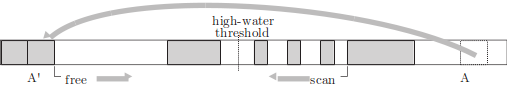
\includegraphics{figures/mrkcmp_1}
  \caption[Ο αλγόριθμος Two-Finger του Edward]
    {Ο αλγόριθμος Two-Finger του Edward. Ζωντανά αντικείμενα
     από την κορυφή του σωρού μετακινούνται σε ελεύθερα κενά
     στη βάση του σωρού. Εδώ το αντικείμενο στη θέση $Α$ έχει
     μετακινηθεί στη θέση $Α'$. Ο αλγόριθμος τερματίζει όταν
     οι δείκτες $scan$ και $free$ συναντηθούν.}
  \label{fig:mrkcmp_1}
\end{figure}

\begin{algorithm}
  \caption{Ο αλγόριθμος συμπύκνωσης Two-Finger}
  \label{alg:mrkcmp_2}
  \begin{algorithmic}[1]
    \Procedure{compact}{\null}
      \State \Call{relocate}{$HeapStart$, $HeapEnd$}
      \State \Call{updateReferences}{$HeapStart$, $free$}
    \EndProcedure
    \Statex
    \Procedure{relocate}{$start$, $end$}
      \State $free \gets start$
      \State $scan \gets end$
      \While{$free < scan$}
        \While{\Call{isMarked}{$free$}}
          \State \Call{unsetMarked}{$free$}
          \State $free \gets free$ $+$ \Call{size}{$free$} \Comment{find next hole}
        \EndWhile
        \While{\textbf{not} \Call{isMarked}{$scan$} \textbf{and} $scan > free$}
          \State $scan \gets scan$ $-$ \Call{size}{$scan$} \Comment{find previous live object}
        \EndWhile
        \If{$scan > free$}
          \State \Call{unsetMarked}{$scan$}
          \State \Call{move}{$scan$, $free$}
          \State $scan \gets free$ \Comment{leave forwarding address (destructively)}
          \State $free \gets free$ $+$ \Call{size}{$free$}
          \State $scan \gets scan$ $-$ \Call{size}{$scan$}
        \EndIf
      \EndWhile
    \EndProcedure
    \Statex
    \Procedure{updateReferences}{$start$, $end$}
      \ForAll{$fld \; \textbf{in} \; Roots$} \Comment{update roots that pointed to moved objects}
        \State $ref \gets *fld$
        \If{$ref > end$}
          \State $*fld \gets ref$ %\Comment{use the forwarding address left in the first pass}
        \EndIf
      \EndFor
      \State $scan \gets start$
      \While{$scan < end$} \Comment{update fields in live region}
        \ForAll{$fld \; \textbf{in} \; Pointers(scan)$}
          \State $ref \gets *fld$
          \If{$ref > end$}
            \State $*fld \gets ref$ \Comment{use the forwarding address left in the first pass}
          \EndIf
        \EndFor
        \State $scan \gets scan$ $+$ \Call{size}{$scan$} \Comment{next object}
      \EndWhile
    \EndProcedure
  \end{algorithmic}
\end{algorithm}

Αλλιώς, το αντικείμενο στη 
θέση $scan$ αντιγράφεται στη θέση $free$, στο παλιό αντίγραφο στη θέση $scan$ αποθηκεύεται 
η νέα διεύθυνση (την τιμή του δείκτη $free$ εκείνη τη χρονική στιγμή) του αντικειμένου και 
η διαδικασία επαναλαμβάνεται. Είναι εμφανές πώς η ποιότητα της συμπύκνωσης εξαρτάται 
πρωτίστως από το εάν το μέγεθος του αντικειμένου στη θέση $scan$ είναι το ίδιο ή σχεδόν το 
ίδιο με το μέγεθος του αντικειμένου στη θέση $free$: αν αυτό δε συμβαίνει, η μνήμη μπορεί 
και πάλι να είναι κατακερματισμένη. Γι αυτόν το λόγο ο αλγόριθμος είναι βέλτιστος στην 
περίπτωση που χρησιμοποιούνται αντικείμενα ίδιου (σταθερού) μεγέθους.

Μετά το πέρας της πρώτης φάσης, ο δείκτης $free$ δείχνει ακριβώς στο σύνορο μεταξύ του 
χρησιμοποιούμενου και του ελεύθερου τμήματος του σωρού. Η δεύτερη φάση αναλαμβάνει να 
ενημερώσει τις τιμές των δεικτών προς τα μετακινηθέντα αντικείμενα: Οι νέες διευθύνσεις 
αυτών βρίσκονται αποθηκεύτηκαν στις παλιές τους θέσεις κατά τη μετακίνησή τους στη 
διάρκεια της πρώτης φάσης.

Στα πλεονεκτήματα του αλγορίθμου περιλαμβάνονται η απλότητα και η ταχύτητα. Επίσης δεν 
παρουσιάζει επιβάρυνση σε χώρο, αφού η νέα διεύθυνση ενός αντικειμένου γράφεται στην παλιά 
του θέση μόνο αφότου έχει ολοκληρωθεί η αντιγραφή του και συνεπώς καμία πληροφορία δεν 
καταστρέφεται. Ο αλγόριθμος υποστηρίζει εσωτερικούς δείκτες. Τέλος, το μοτίβο πρόσβασης 
στη μνήμη είναι σχετικά προβλέψιμο, κάτι που σημαίνει πώς η προφόρτωση (υλικού ή/και 
λογισμικού) μπορεί να οδηγήσει το συλλέκτη σε καλή συμπεριφορά ως προς τη μνήμη cache. 
Ωστόσο, το βασικό μειονέκτημα παραμένει: τα αντικείμενα τοποθετούνται σε τυχαία σειρά στο 
σωρό και αυτό καταστρέφει την όποια τοπικότητα του τροποποιητή.

\section{Ο αλγόριθμος Lisp 2}
Ο επόμενος αλγόριθμος που εξετάζουμε συμπυκνώνει τα αντικείμενα διατηρώντας την αρχική 
τους διάταξη και είναι ο Lisp 2. Ο αλγόριθμος χρησιμοποιείται ευρύτατα, είτε στην αρχική 
του μορφή, είτε παραλλαγμένος ώστε να εκτελείται παράλληλα \cite{DBLP:conf/jvm/FloodDSZ01}. 
Μπορεί να χρησιμοποιηθεί σε εφαρμογές όπου ο σωρός φιλοξενεί αντικείμενα διαφορετικών 
μεγεθών και παρότι πραγματοποιεί τρία περάσματα στο σωρό, κάθε ένα από αυτά κάνει λίγη 
δουλειά. Παρότι γενικά οι αλγόριθμοι συλλογής με σήμανση και συμπύκνωση φημίζονται για τη 
χαμηλή διεκπεραιωτική τους ικανότητα, οι Cohen και Nicolau \cite{DBLP:journals/toplas/CohenN83}
διαπίστωσαν πώς επρόκειτο για το γρηγορότερο από του αλγορίθμους που συνέκριναν .
Το βασικό του μειονέκτημα είναι πώς απαιτεί μία επιπλέον λέξη στην επικεφαλίδα ενός 
αντικειμένου για την αποθήκευση της νέας διεύθυνσης στην οποία αυτό θα μετακινηθεί. Το 
πεδίο αυτό μπορεί να χρησιμοποιηθεί για την αποθήκευση του bit σήμανσης.

Το πρώτο πέρασμα του αλγορίθμου (μετά από τη φάση της σήμανσης) υπολογίζει τη διεύθυνση 
στην οποία θα μετακινηθεί κάθε ζωντανό αντικείμενο και αποθηκεύει την τιμή αυτή στο πεδίο 
$forwardingAddress$ αυτού. Η διαδικασία \textenglish{\textproc{computeLocations}}, η οποία πραγματοποιεί 
το πρώτο πέρασμα, δέχεται τρία ορίσματα: την αρχική και τελική διεύθυνση του προς 
συμπκύκνωση τμήματος του σωρού (περιοχή προέλευσης) καθώς και την αρχική διεύθυνση του 
τμήματος του σωρού όπου θα μετακινηθούν τα αντικείμενα (περιοχή προορισμού). Παρότι συνήθως 
η περιοχή προορισμού ταυτίζεται με την περιοχή προέλευσης, αν η συμπύκνωση εκτελείται 
παράλληλα, κάθε νήμα δύναται να διατηρεί τις δικές του διακριτές περιοχές. Η διαδικασία 
\textenglish{\textproc{computeLocations}} διατηρεί δύο δείκτες στο σωρό: ο δείκτης $scan$ διατρέχει 
σειριακά το σωρό, εξετάζοντας κάθε αντικείμενο (σημασμένο και μή) στην περιοχή προέλευσης, 
ενώ ο δείκτης $free$ δείχνει στην πρώτη ελεύθερη θέση στην περιοχή προορισμού. Αν ένα 
αντικείμενο είναι ζωντανό, τότε θα μετακινηθεί (τελικά) στη θέση $free$ και έτσι η τρέχουσα
τιμή του δείκτη free αποθηκεύεται στο πεδίο $forwardingAddress$ του αντικειμένου και κατόπιν 
αυξάνεται κατά το μέγεθος αυτού. Αν πάλι είναι νεκρό, απλώς αγνοείται.

Το δεύτερο πέρασμα πραγματοποιείται από τη διαδικασία \textenglish{\textproc{updateReferences}},
κατά την εκτέλεση της οποίας ενημερώνονται οι ρίζες των νημάτων του τροποποιητή καθώς και τα πεδία
δείκτες σημασμένων αντικειμένων ώστε να δείχνουν στις νέες διευθύνσεις των αντικειμένων προς 
τα οποία δείχνουν, χρησιμοποιώντας την τιμή που αποθηκεύθηκε στο πεδίο $forwarding\-Address$ 
των τελευταίων στη διάρκεια του πρώτου περάσματος. 

\begin{algorithm}
  \caption{Ο αλγόριθμος συμπύκνωσης Lisp 2}
  \label{alg:mrkcmp_3}
  \begin{algorithmic}[1]
    \Procedure{compact}{\null}
      \State \Call{computeLocations}{$HeapStart$, $HeapEnd$, $HeapStart$}
      \State \Call{updateReferences}{$HeapStart$, $HeapEnd$}
      \State \Call{relocate}{$HeapStart$, $HeapEnd$}
    \EndProcedure
    \Statex
    \Procedure{computeLocations}{$start$, $end$, $toRegion$}
      \State $scan \gets start$
      \State $free \gets toRegion$
      \While{$scan < end$}
        \If{\Call{isMarked}{$scan$}}
          \State \Call{forwardingAddress}{$scan$} $\gets free$
          \State $free \gets free$ $+$ \Call{size}{$scan$}
        \EndIf
        \State $scan \gets scan$ $+$ \Call{size}{$scan$}
      \EndWhile
    \EndProcedure
    \Statex
    \Procedure{updateReferences}{$start$, $end$}
      \ForAll{$fld \; \textbf{in} \; Roots$}
        \State $ref \gets *fld$
        \If{$ref \neq \textbf{null}$}
          \State $*fld \gets$ \Call{forwardingAddress}{$ref$}
        \EndIf
      \EndFor
      \State $scan \gets start$
      \While{$scan < end$}
        \If{$\Call{isMarked}{scan}$}
          \ForAll{$fld \; \textbf{in} \; Pointers(scan)$}
            \If{$*fld \neq \textbf{null}$}
              \State $*fld \gets$ \Call{forwardingAddress}{$*fld$}
             \EndIf
            \EndFor
          \EndIf
        \State $scan \gets scan +$ \Call{size}{$scan$}
      \EndWhile
    \EndProcedure
    \Statex
    \Procedure{relocate}{$start$, $end$}
      \State $scan \gets start$
      \While{$scan < end$} 
        \If{\Call{isMarked}{$child$}}
          \State $dest \gets$ \Call{setMarked}{$child$}
          \State \Call{move}{$scan$, $dest$}
          \State \Call{unsetMarked}{$dest$}
        \EndIf
        \State $scan \gets scan$ $+$ \Call{size}{$scan$}
      \EndWhile
    \EndProcedure
  \end{algorithmic}
\end{algorithm}    

Στο τρίτο και τελευταίο πέρασμα, η διαδικασία \textenglish{\textproc{relocate}} μετακινεί κάθε ζωντανό 
(σημασμένο) αντικείμενο στη νέα του διεύθυνση.

\section{Συμπύκνωση με ένα πέρασμα}
Εάν θέλουμε να μειώσουμε τον αριθμό των περασμάτων στο σωρό σε δύο (ένα για 
σήμανση και ένα για ολίσθηση αντικειμένων), τότε πρέπει να αποθηκεύσουμε τις 
διευθύνσεις προορισμού σε ένα βοηθητικό πίνακα ο οποίος διατηρείται κατά τη 
διάρκεια της συμπύκνωσης. Οι αλγόριθμοι με σήμανση και συμπύκνωση που σχεδίασαν 
οι Abuaiadh κ.ά. \cite{DBLP:conf/oopsla/AbuaiadhOPS04} καθώς και οι Kermany και 
Petrank \cite{DBLP:conf/pldi/KermanyP06} επιτυγχάνουν υψηλές επιδόσεις σε 
πολυεπεξεργαστικά συστήματα ακολουθώντας αυτήν ακριβώς την τεχνική. Ο πρώτος 
αλγόριθμος είναι παράλληλος (ο συλλέκτης χρησιμοποιεί πολλαπλά νήματα ενώ τα 
νήματα του τροποποιητή είναι σταματημένα), ενώ ο δεύτερος δύναται να διαμορφωθεί 
τόσο για ταυτόχρονη εκτέλεση (επιτρέποντας ταυτόχρονη εκτέλεση των νημάτων 
συλλέκτη και τροποποιητή) όσο και για αυξητική εκτέλεση (όπου η εκτέλεση του
τροποποιητή αναστέλλεται περιοδικά για ένα βραχύ χρονικό διάστημα κατά το οποίο
επιτρέπεται στο συλλέκτη η εκτέλεση ενός μικρού κβάντου εργασιών). 

\begin{figure}
  \centering
  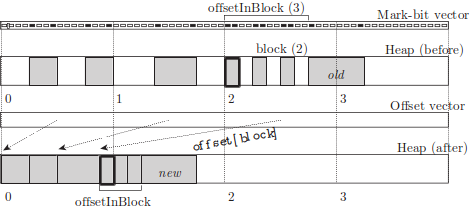
\includegraphics{figures/mrkcmp_2}
  \caption[Ο σωρός (πριν και μετά τη συμπύκνωση) και τα μεταδεδομένα
           που χρησιμοποιεί ο αλγόριθμος Compressor.]
    {Ο σωρός (πριν και μετά τη συμπύκνωση) και τα μεταδεδομένα
     που χρησιμοποιεί ο αλγόριθμος Compressor. Τα bits του διανύσματος
     σήμανσης υποδεικνύουν την αρχή και το τέλος κάθε ζωντανού
     αντικειμένου. Οι λέξεις στο διάνυσμα μετατόπισης αποθηκεύουν
     τη διεύθυνση προς την οποία θα μετακινηθεί το πρώτο ζωντανό
     αντικείμενο του αντίστοιχου μπλοκ. Οι διευθύνσεις προώθησης
     δεν αποθηκεύονται αλλά υπολογίζονται όταν αυτό είναι απαραίτητο
     από τα διανύσματα σήμανσης και μετατόπισης.}
  \label{fig:mrkcmp_2}
\end{figure}

Στην ενότητα αυτή εξετάζουμε την απλή εκδοχή του αλγορίθμου, όπου και υποθέτουμε πώς
διακόπτεται η εκτέλεση των νημάτων του τροποποιητή κατά την εκτέλεση του
συλλέκτη.

Η λειτουργία του αλγορίθμου στηρίζεται κυρίως στη χρήση βοηθητικών πινάκων ή και
διανυσμάτων. Όπως και πολλοί συλλέκτες, ο αλγόριθμος Compressor χρησιμοποιεί ως
διάνυσμα σήμανσης μια δομή bitmap όπου κάθε bit αντιστοιχεί σε μία λέξη μνήμης. 
Η φάση της σήμανσης θέτει σε λογικό ένα τα bit που αντιστοιχούν στην πρώτη και 
τελευταία λέξη ενός ζωντανού αντικειμένου. Εξετάζοντας τη δομή αυτή, ο συλλέκτης 
είναι σε θέση να προσδιορίσει κατά τη διάρκεια της συμπύκνωσης το μέγεθος ενός 
οιουδήποτε (ζωντανού) αντικειμένου.

Επιπλέον, ο αλγόριθμος χρησιμοποιεί έναν πίνακα όπου αποθηκεύει τις διευθύνσεις
προορισμού των αντικειμένων. Καθώς η αποθήκευση της διεύθυνσης κάθε ενός
αντικειμένου ξεχωριστά θα ήταν απαγορευτική, ο αλγόριθμος διαιρεί το σωρό σε
μικρά, ισομεγέθη μπλοκ με τυπικό μέγεθος 256 ή 512 bytes. Ο πίνακας $offset$
αποθηκεύει τη διεύθυνση προορισμού του πρώτου αντικειμένου για κάθε μπλοκ.
Οι νέες διευθύνσεις των υπολοίπων ζωντανών αντικειμένων μπορούν να υπολογισθούν
με χρήση του πίνακα $offset$ και του διανύσματος σήμανσης. Ομοίως, δοθείσης μιας 
αναφοράς προς ένα αντικείμενο, μπορούμε να υπολογίσουμε το μπλοκ στο οποίο
αντιστοιχεί και επομένως να εξάγουμε τη διεύθυνση προορισμού από την κατάλληλη
καταχώριση στον πίνακα $offset$ και τα bit σήμανσης για αυτό το μπλοκ. Αυτό
επιτρέπει στον αλγόριθμο να αντικαταστήσει τα πολλαπλά περάσματα στο σωρό για
μετακίνηση αντικειμένων και επιδιόρθωση δεικτών με ένα απλό και γρήγορο πέρασμα
του διανύσματος σήμανσης για την κατασκευή του πίνακα $offset$, καθώς και άλλο 
ένα πέρασμα για τη μετακίνηση αντικειμένων και την ενημέρωση των δεικτών 
συμβουλευόμενος τις βοηθητικές αυτές δομές.

\begin{algorithm}
  \caption{Ο αλγόριθμος συμπύκνωσης Compressor}
  \label{alg:mrkcmp_4}
  \begin{algorithmic}[1]
    \Procedure{compact}{\null}
      \State \Call{computeLocations}{$HeapStart$, $HeapEnd$, $HeapStart$}
      \State \Call{updateReferencesRelocate}{$HeapStart$, $HeapEnd$}
    \EndProcedure
    \Statex
    \Procedure{computeLocations}{$start$, $end$, $toRegion$}
      \For{$b \gets 0 \; \textbf{to} \; numBits(start, end)-1$}
        \If{$b \bmod BITS\_IN\_BLOCK = 0$}
          \Comment{crossed boundary?}
          \State $offset[block] \gets loc$
          \Comment{first object will be moved to loc}
          \State $block \gets block+1$
        \EndIf
        \If{$bitmap[b] = MARKED$}
          \State $loc \gets loc + BYTES\_PER\_BIT$
          \Comment{advance by size of live objects}
        \EndIf
      \EndFor
    \EndProcedure
    \Statex
    \Procedure{newAddress}{$old$}
      \State $block \gets$ \Call{getBlockNum}{$old$}
      \State \Return{$offset[block]$ $+$ \Call{offsetInBlock}{$old$}}
    \EndProcedure
    \Statex
    \Procedure{updateReferencesRelocate}{$start$, $end$}
      \ForAll{$fld \; \textbf{in} \; Roots$}
        \State $ref \gets *fld$
        \If{$ref \neq \textbf{null}$}
          \State $*fld \gets$ \Call{newAddress}{$ref$}
        \EndIf
      \EndFor
      \State $scan \gets start$
      \While{$scan < end$}
        \State $scan \gets$ \Call{nextMarkedObject}{$scan$}
        \Comment{use the bitmap}  
        \ForAll{$fld \; \textbf{in} \; Pointers(scan)$}
          \Comment{update references}
          \State $ref \gets *fld$
          \If{$ref \neq \textbf{null}$}
            \State $*fld \gets$ \Call{newAddress}{$ref$}
          \EndIf
        \EndFor
        \State $dest \gets$ \Call{newAddress}{$scan$}
        \State \Call{move}{$scan$, $dest$}
      \EndWhile
    \EndProcedure
  \end{algorithmic}
\end{algorithm}

Αφού η ρουτίνα \textenglish{\textproc{computeLocations}} υπολογίσει το πίνακα $offset$, η 
ρουτίνα \textenglish{\textproc{updateReferencesRelocate}} ενημερώνει αρχικά τους δείκτες των 
αντικειμένων ριζών. Ο αλγόριθμος Lisp 2 ξεχωρίζει τα περάσματα της μετακίνησης
αντικειμένων και της ενημέρωσης δεικτών, καθώς οι πληροφορίες της μετακίνησης
αποθηκεύονται στο σωρό και χάνονται κατά τη μετακίνηση αντικειμένων. Αντίθετα,
ο αλγόριθμος Compressor μετακινεί τα ζωντανά αντικείμενα και ενημερώνει τους
δείκτες σε ένα μόνο πέρασμα, καθώς οι νέες διευθύνσεις των αντικειμένων
υπολογίζονται εύκολα από τον πίνακα $offset$ και το bitmap σήμανσης και δε
χρειάζεται να αποθηκευθούν στο σωρό. Η ρουτίνα \textenglish{\textproc{newAddress}} υπολογίζει
τη νέα διεύθυνση ενός ζωντανού αντικειμένου. Αρχικά υπολογίζει το
μπλοκ στο οποίο ευρίσκεται το αντικείμενο και χρησιμοποιεί την τιμή ως index
στον πίνακα $offset$ ώστε να βρει τη διεύθυνση προορισμού του \textbf{πρώτου}
ενεργού αντικειμένου στο συγκεκριμένο block. Η νέα διεύθυνση του αντικειμένου
προκύπτει προσθέτοντας στην προηγούμενη τιμή το μέγεθος σε λέξεις των ζωντανών
αντικειμένων που προηγούνται του αντικειμένου στο μπλοκ, δεδομένο που υπολογίζει
συμβουλευόμενη το bitmap που αντιστοιχεί στο εν λόγω μπλοκ.

\section{Θέματα προς εξέταση}
\subsection{Είναι απαραίτητη η συμπύκνωση;}
Η συλλογή με σήμανση και εκκαθάριση έχει μικρότερες απαιτήσεις σε μνήμη από ότι 
άλλες τεχνικές όπως η συλλογή με αντιγραφή. Επιπλέον, καθώς δεν μετακινεί 
αντικείμενα, ένας συλλέκτης με σήμανση και εκκαθάριση αρκείται στο να εντοπίσει 
τα προσβάσιμα από τις ρίζες αντικείμενα και να τα σημάνει: δεν τα μεταβάλλει. 
Περιβάλλοντα όπου το σύστημα εκτέλεσης δε μπορεί να παρέχει έγκυρη πληροφορία 
τύπων ώστε να προσδιοριστούν με βεβαιότητα οι μεταβλητές δείκτες δυσχεραίνουν 
τον προσδιορισμό και τη σήμανση αντικειμένων που είναι προσβάσιμα από τις ρίζες 
του τροποποιητή. Παρόλα αυτά, το σημαντικότερο μειονέκτημα ενός συλλέκτη με σήμανση 
και εκκαθάριση είναι η τάση του να κατακερματίζει τη μνήμη. Η χρήση προηγμένων 
τεχνικών για την εκχώρηση μνήμης όπως η χρήση ξεχωριστών συνδεδεμένων ελεύθερων λιστών 
για αντικείμενα διαφορετικού μεγέθους (segregated-fits lists) μειώνει την 
πιθανότητα για κατακερματισμό της μνήμης μόνο σε εφαρμογές με μικρές απαιτήσεις σε 
μεγάλα αντικείμενα και με σχετικά μη μεταβλητή αναλογία μεγεθών αντικειμένων. Σε 
μία τυπική εφαρμογή η οποία τρέχει για πολύ χρόνο και στην οποία χρησιμοποιούνται 
αντικείμενα διαφόρων μεγεθών, ο κατακερματισμός που επιφέρει ένας μη-μετακινών 
συλλέκτης αποτελεί πηγή προβλημάτων. Γι αυτόν το λόγο, οι περισσότερες εμπορικές 
υλοποιήσεις της εικονικής μηχανής της γλώσσας Java χρησιμοποιούν μετακινούντες 
συλλέκτες που συμπυκνώνουν το σωρό.

\subsection{Επίδραση στη ρυθμαπόδοση}
Η συλλογή με σήμανση και συμπύκνωση ωστόσο τείνει να είναι πιο αργή από τη 
συλλογή με σήμανση και εκκαθάριση ή τη συλλογή με αντιγραφή. Ο λόγος είναι πώς 
με εξαίρεση με τον αλγόριθμο Compressor, o συλλέκτης πραγματοποιεί πολλαπλά 
περάσματα στο σωρό, με το κάθε πέρασμα να είναι ακριβό. Ο Printezis \cite{DBLP:conf/jvm/Printezis01}
και o Soman κ.ά. \cite{DBLP:conf/iwmm/SomanKB04} προτείνουν τη χρήση
προσαρμοστικής συλλογής σκουπιδιών: ο συλλέκτης εκτελεί τον αλγόριθμο
με σήμανση και εκκαθάριση και προσφεύγει στον αλγόριθμο με σήμανση και συμπύκνωση
όταν οι μετρικές κατακερματισμού υποδεικνύουν πώς η αλλαγή θα είναι επικερδής.

\subsection{Μακρόβια αντικείμενα}
Δεν είναι ασυνήθιστο για αντικείμενα που ζουν πολύ ή είναι αθάνατα (δηλαδή ζουν
καθ'~όλη τη διάρκεια εκτέλεσης του τροποποιητή) να συσσωρεύονται στην αρχή του
σωρού από μετακινούντες συλλέκτες. Οι συλλέκτες με αντιγραφή διαχειρίζονται μη
αποδοτικά τα αντικείμενα αυτά, αντιγράφοντάς τα συνέχεια από τον ένα ημιχώρο
στον άλλον. Από την άλλη πλευρά, οι γενεαλογικοί συλλέκτες (τους οποίους
εξετάζουμε στο κεφάλαιο 6), τα προωθούν σε διαφορετικό τμήμα του σωρού, το
οποίο και συλλέγεται σπανίως. Η γενεαλογική συλλογή σκουπιδιών ωστόσο δεν
ενδείκνυται πάντα και ιδιαίτερα όταν ο σωρός είναι σχεδόν γεμάτος. Επίσης δε
λύνει το πρόβλημα αν τα αντικείμενα βρίσκονται ήδη αποθηκευμένα στην παλαιότερη
γενεά. Η συλλογή με σήμανση και συμπύκνωση μπορεί να επιλέξει τη μη συμπύκνωση
αυτού του ``ιζήματος''. O Hanson \cite{DBLP:journals/spe/Hanson77} πρώτος
παρατήρησε την εμφάνιση του προβλήματος στο σύστημα SITBOL, το οποίο αποτελούσε
μία υλοποίηση της γλώσσας SNOBOL4 για αρχιτεκτονική DEC-10. O Hanson πρότεινε
τη δυναμική μέτρηση του μεγέθους του 'ιζήματος' και τη μη συλλογή αυτού εκτός
και αν είναι τελείως απαραίτητη, με τίμημα ένα μικρό ποσοστό κατακερματισμού.

\subsection{Τοπικότητα}
Όπως είδαμε, οι συλλέκτες με σήμανση και συμπύκνωση μπορεί να διατηρούν τη
διάταξη των αντικειμένων στο σωρό είτε να τα αναδιατάσσουν τυχαία. Παρότι
οι δεύτεροι είναι ταχύτεροι και χωρίς κόστος σε χώρο, η τοπικότητα του
τροποποιητή ενδέχεται να καταστραφεί τελείως από την τυχαία διάταξη των
αντικειμένων. Η ολισθαίνουσα συμπύκνωση έχει τέλος ένα ακόμη πλεονέκτημα:
η ανάκτηση της συνολικής μνήμης που καταλαμβάνεται από αντικείμενα μετά
από ένα συγκεκριμένο όριο στο σωρό δύναται να ανακτηθεί αμέσως με μία απλή
μείωση του δείκτη $free$.

\subsection{Περιορισμοί}
Στη βιβλιογραφία έχει προταθεί μια πληθώρα αλγορίθμων συλλογής
με σήμανση και συμπύκνωση. Πολλοί από αυτούς ωστόσο έχουν
ιδιότητες μη επιθυμητές και σε αρκετές περιπτώσεις απαράδεκτες.
Ένα από τα ζητήματα αφορά το κόστος σε χώρο που επιβάλλει
η ανάγκη αποθήκευσης των διευθύνσεων προώθησης (παρότι αυτό
είναι μικρότερο από το αντίστοιχο κόστος της συλλογής με
αντιγραφή). Μερικοί αλγόριθμοι συμπύκνωσης επιβάλλουν περιορισμούς
στον τροποποιητή. Απλοί αλγόριθμοι όπως ο Two-Finger μπορούν
να διαχειριστούν μόνο αντικείμενα του ίδιου μεγέθους. Εφόσον
λοιπόν είναι δυνατός ο διαχωρισμός των αντικειμένων με βάση
το μέγεθός τους, σε ποιο βαθμό είναι απαραίτητη η συμπύκνωση;
Τέλος, οι περισσότεροι αλγόριθμοι συμπύκνωσης αποκλείουν τη
χρήση εσωτερικών δεικτών: ο αλγόριθμος Two-Finger αποτελεί
εξαίρεση.

\end{greek}

\begin{greek}
\chapter{Συλλογή σκουπιδιών με αντιγραφή}\label{ch:cop}
Η συλλογή με σήμανση και εκκαθάριση έχει σχετικά μικρό κόστος,
ωστόσο ενδέχεται η μνήμη να κατακερματίζεται. Η συλλογή σκουπιδιών
πρέπει να καταλαμβάνει τον ελάχιστο δυνατό χρόνο εκτέλεσης σε
ένα καλώς διαμορφωμένο σύστημα και καθώς το κόστος των εργασιών 
μνήμης του τροποποιητή κυριαρχεί έναντι αυτού του συλλέκτη η
εκχώρηση μνήμης πρέπει να είναι γρήγορη. Η συλλογή με σήμανση
και συμπύκνωση εξαλείφει τον κατακερματισμό της μνήμης και 
υποστηρίζει πολύ γρήγορη εκχώρηση μνήμης με τίμημα την αύξηση 
του χρόνου συλλογής αφού ο σωρός διατρέχεται πολλές φορές. Στο 
παρόν κεφάλαιο παρουσιάζεται η \textbf{συλλογή σκουπιδιών με 
αντιγραφή}, η οποία ανακαλύφθηκε 
από τους Fenichel και Yochelson \cite{DBLP:journals/cacm/FenichelY69} 
και Cheney \cite{DBLP:journals/cacm/Cheney70}. Η συλλογή με 
αντιγραφή συμπυκνώνει το σωρό, επιτρέποντας γρήγορη εκχώρηση
μνήμης και επίσης πραγματοποιεί μόνο ένα πέρασμα στο σωρό. Το 
βασικό μειονέκτημα είναι πώς το μέγεθος της διαθέσιμης μνήμης 
στο σωρό μειώνεται στο μισό.

\section{Αντιγραφή μεταξύ ημιχώρων}
Η βασική εκδοχή ενός συλλέκτη αντιγραφής διαιρεί το σωρό σε δύο 
ισομεγέθεις \textbf{ημιχώρους}, το \textbf{χώρο-από} και το \textbf{χώρο-προς}.
Εάν υπάρχει διαθέσιμη μνήμη για ένα αντικείμενο, αυτή εκχωρείται στο χώρο-προς 
αυξάνοντας την τιμή ενός δείκτη $free$. Διαφορετικά, ο ρόλος των 
ημιχώρων εναλλάσσεται πριν ο συλλέκτης αντιγράψει όλα τα ζωντανά 
αντικείμενα από τον πρώην χώρο-προς (και νυν χώρο-από) στο νυν 
χώρο-προς (πρώην χώρο-από). Στο τέλος της συλλογής, όλα τα ζωντανά 
αντικείμενα είναι τοποθετημένα σε ένα πυκνό πρόθεμα του χώρου-προς. 
Ο συλλέκτης αγνοεί το χώρο-από και τα αντικείμενα που βρίσκονται σε 
αυτόν μέχρι την επόμενη συλλογή. Στην πράξη βέβαια, οι περισσότεροι 
συλλέκτες αντιγραφής μηδενίζουν το χώρο-από για ασφάλεια κατά την
αρχικοποίηση του επόμενου κύκλου συλλογής. 

Μετά την αρχικοποίηση, οι συλλέκτες αντιγραφής αντιγράφουν τα 
αντικείμενα ρίζες στο χώρο-προς. Τα αντικείμενα που έχουν αντιγραφεί 
αλλά όχι ακόμα εξεταστεί είναι γκρι. Κάθε πεδίο δείκτης ενός 
γκρι αντικειμένου περιέχει είτε την τιμή \textbf{null} είτε μία 
αναφορά προς ένα αντικείμενο του χώρου-από. Η διαδικασία \textenglish{\textproc{scan}}
ενημερώνει κάθε πεδίο δείκτη ενός γκρι αντικειμένου, ο οποίος 
δείχνει σε κάποιο αντικείμενο του χώρου-από, με τη διεύθυνση 
του αντιγράφου του αντικειμένου στο χώρο-προς. 

\begin{algorithm}
  \caption{Συλλογή σκουπιδιών με αντιγραφή ημιχώρων: αρχικοποίηση και εκχώρηση}
  \label{alg:cop_1}
  \begin{algorithmic}[1]
    \Procedure{createSemispaces}{\null}
      \State $tospace \gets HeapStart$
      \State $extent \gets (HeapEnd-HeapStart)/2$ \Comment{size of a semispace}
      \State $top \gets fromspace$
      \State $free \gets tospace$
    \EndProcedure
    \Statex
    \Function{allocate}{$size$}
      \State \textbf{atomic}
      \State $result \gets free$
      \State $newfree \gets result + size$
      \If{$newFree > top$}
        \State \Return{\textbf{null}} \Comment{signal ``memory exhausted''}
      \EndIf
      \State $free \gets newfree$
      \State \Return{$result$}
    \EndFunction
  \end{algorithmic}
\end{algorithm}

Πιο συγκεκριμένα, 
για κάθε πεδίο δείκτη του ορίσματος της, καλεί τη διαδικασία 
\textenglish{\textproc{process}}, η οποία με τη σειρά της, αν το όρισμα της 
δεν περιέχει την τιμή \textbf{null}, καλεί τη συνάρτηση \textenglish{\textproc{forward}} 
με όρισμα το όρισμα με το οποίο αυτή κλήθηκε. Η συνάρτηση \textenglish{\textproc{forward}} 
ελέγχει αν το αντικείμενο αναφοράς του ορίσματος της έχει ήδη 
αντιγραφεί στο χώρο-προς, και αν ναι, τότε επιστρέφει τη διεύθυνση 
του αντιγράφου. Αν όχι, καλεί τη συνάρτηση \textenglish{\textproc{copy}} η 
οποία εκτελεί τις εξής ενέργειες: αποθηκεύει στη μεταβλητή $toRef$ 
την τιμή του δείκτη $free$, αυξάνει το δείκτη $free$ κατά το 
μέγεθος του αντικειμένου (όπως ακριβώς συμβαίνει και κατά την 
εκχώρηση μνήμης), μετακινεί (αντιγράφει) το αντικείμενο στη θέση 
$toRef$, αποθηκεύει στο πεδίο $forwardingAddress$ του αντικειμένου 
τη διεύθυνση του αντιγράφου του $toRef$ και τέλος, πριν επιστρέψει
τη μεταβλητή $toRef$, την προσθέτει στη λίστα εργασιών. Η αποθήκευση 
της διεύθυνσης ενός αντικειμένου στο πεδίο $forwardingAddress$ 
του αντιγράφου του στο χώρο-από από τη συνάρτηση \textenglish{\textproc{copy}} 
εξασφαλίζει πώς η συλλογή με αντιγραφή διατηρεί την τοπολογία των 
ζωντανών αντικειμένων κατά την αντιγραφή τους από το χώρο-από στο
χώρο-προς. Σε αντίθεση με τους περισσότερους συλλέκτες με σήμανση 
και συμπύκνωση, ένας συλλέκτης με αντιγραφή δεν απαιτεί κανένα 
επιπλέον πεδίο στην επικεφαλίδα ενός αντικειμένου. Οποιοδήποτε 
πεδίο στο αντίγραφο ενός αντικειμένου του χώρου-προς στο χώρο-από 
μπορεί να αποθηκεύσει τη διεύθυνση του αντικειμένου στο χώρο-προς, 
καθώς το αντίγραφο αυτό δεν πρόκειται να χρησιμοποιηθεί ξανά 
μετά το πέρας της συλλογής. Το γεγονός αυτό καθιστά τη συλλογή 
με αντιγραφή κατάλληλη ακόμη και για αντικείμενα χωρίς επικεφαλίδα.

Όπως και οι περισσότερες τεχνικές συλλογής σκουπιδιών με εξιχνίαση, 
έτσι και η συλλογή με αντιγραφή διατηρεί μια λίστα εργασιών την 
οποία και επεξεργάζεται μέχρις ότου αυτή εκκενωθεί. Η λίστα εργασιών 
δύναται να υλοποιηθεί με διαφορετικούς τρόπους, οδηγώντας σε
διαφορετική σειρά διάσχισης του γράφου αντικειμένων και διαφορετικές
απαιτήσεις σε χώρο. Οι Fenichel και Yochelson \cite{DBLP:journals/cacm/FenichelY69}
υλοποιούν τη λίστα εργασιών ως μία απλή βοηθητική στοίβα, όπως 
κάνουν οι συλλέκτες με σήμανση και εκκαθάριση. Η αντιγραφή τελειώνει 
όταν η στοίβα είναι άδεια.

\begin{algorithm}
  \caption{Συλλογή σκουπιδιών με αντιγραφή ημιχώρων}
  \label{alg:cop_2}
  \begin{algorithmic}[1]
    \Procedure{collect}{\null}
      \State \Call{flip}{\null}
      \State \Call{initialize}{$worklist$} \Comment{empty}
      \ForAll{$fld \; \textbf{in} \; Roots$} \Comment{copy the roots}
        \State \Call{process}{$fld$}
      \EndFor
      \While{\textbf{not} \Call{isEmpty}{$worklist$}} \Comment{copy transitive closure}
        \State $ref \gets$ \Call{remove}{$worklist$}
        \State \Call{scan}{$ref$}
      \EndWhile    
    \EndProcedure
    \Statex
    \Procedure{flip}{\null}
      \Comment{switch semispaces}
      \State $fromspace, tospace \gets tospace, \, fromspace$
       \State $top \gets tospace + extent$
      \State $free \gets tospace$
    \EndProcedure  
    \Statex
    \Procedure{scan}{$ref$}
      \ForAll{$fld \; \textbf{in} \; Pointers(Roots)$}
        \State \Call{process}{$fld$}      
      \EndFor
    \EndProcedure
    \Statex
    \Procedure{process}{$fld$} \Comment{update field with reference to tospace replica}
      \State $fromRef \gets *fld$
      \If{$fromRef \neq \textbf{null}$}
        \State $*fld \gets$ \Call{forward}{$fromRef$} \Comment{update with tospace reference}
      \EndIf
    \EndProcedure
    \Statex
    \Function{forward}{$fromRef$}
      \State $toRef \gets$ \Call{forwardingAddress}{$fromRef$}
      \If{$toRef = \textbf{null}$} \Comment{not copied (not marked)}
        \State $toRef \gets$ \Call{copy}{$fromRef$}
      \EndIf
      \State \Return{$toRef$}
    \EndFunction
    \Statex                                                  
    \Function{copy}{$fromRef$} \Comment{copy object and return forwarding address}
      \State $toRef \gets free$
      \State $free \gets free$ $+$ \Call{size}{$fromRef$}
      \State \Call{move}{$fromRef$, $toRef$}
      \State \Call{forwardingAddress}{$fromRef$} $\gets toRef$ \Comment{mark}
      \State \Call{add}{$worklist$, $toRef$}
      \State \Return{$toRef$}
    \EndFunction
  \end{algorithmic}
\end{algorithm}

Ο αλγόριθμος του Cheney \cite{DBLP:journals/cacm/Cheney70} χρησιμοποιεί
τα γκρι αντικείμενα του χώρου-προς ως μία ουρά. Η μόνη επιπλέον
μεταβλητή που χρησιμοποιεί είναι ο δείκτης $scan$, ο οποίος κάθε
χρονική στιγμή αναφέρεται στο επόμενο μη σαρωμένο αντικείμενο.
Όταν οι δύο ημιχώροι εναλλάσσονται οι δείκτες $scan$ και $free$
αρχικοποιούνται ώστε να δείχνουν στην αρχή του χώρου-προς (η
διαδικασία \textenglish{\textproc{initialize}} εγγράφει το δείκτη $scan$ με
την τιμή του δείκτη $free$, ο οποίος στη διαδικασία \textenglish{\textproc{flip}}
ενημερώθηκε με την διεύθυνση της αρχής του ημιχώρου-προς).
Αφού αντιγραφούν τα αντικείμενα ρίζες, η λίστα εργασιών, δηλαδή
το σύνολο των γκρι αντικειμένων αποτελείται ακριβώς από τα
αντιγεγραμμένα και όχι ακόμη σαρωμένα αντικείμενα στο χώρο-προς
μεταξύ των δεικτών $scan$ και $free$. Αυτή ακριβώς είναι και η
αναλλοίωτη που διατηρείται κατά τη διάρκεια της συλλογής. Ο
δείκτης $scan$ αυξάνεται καθώς πεδία αντικειμένων του χώρου-προς
σαρώνονται και ενημερώνονται. Η συλλογή ολοκληρώνεται όταν η
λίστα εργασιών είναι κενή: όταν ο δείκτης $scan$ συναντήσει το
δείκτη $free$. Η υλοποίηση είναι πολύ απλή: η συνάρτηση \textenglish{\textproc{isEmpty}}
συγκρίνει τις τιμές των δεικτών $scan$ και $free$, η συνάρτηση
\textenglish{\textproc{remove}} απλώς επιστρέφει την τιμή του δείκτη $scan$
και τέλος η διαδικασία \textenglish{\textproc{add}} δεν προβαίνει σε καμία
ενέργεια.

\begin{algorithm}
  \caption{Αντιγραφή με χρήση της λίστας εργασιών του Cheney}
  \label{alg:c_3}
  \begin{algorithmic}[1]
    \Procedure{initialize}{\null}
      \State $scan \gets free$
    \EndProcedure
    \Statex
    \Function{isEmpty}{$worklist$}
      \State \Return{$scan = free$}
    \EndFunction
    \Statex
    \Function{remove}{$worklist$}
      \State $ref \gets scan$
      \State $scan \gets scan$ $+$ \Call{size}{$scan$}
      \State \Return{$ref$}
    \EndFunction
    \Statex
    \Procedure{add}{$worklist$, $ref$}
      \State /* $nop$ */
    \EndProcedure
  \end{algorithmic}
\end{algorithm}

\section{Σειρά διάταξης και τοπικότητα}
Η τοπικότητα τόσο του τροποποιητή όσο και του συλλέκτη μπορεί
να έχει σημαντική επίδραση στην επίδοση ενός προγράμματος. Όπως
είδαμε στο προηγούμενο κεφάλαιο ο συλλέκτης μπορεί να βλάψει
την τοπικότητα του τροποποιητή και επομένως και την επίδοση 
του τελευταίου εάν μετακινεί αντικείμενα σε τυχαίες νέες θέσεις 
χωρίς να λαμβάνει υπόψη σχέσεις μεταξύ δεικτών ή την αρχική 
διάταξη των αντικειμένων \cite{DBLP:conf/oopsla/AbuaiadhOPS04}. 
Ωστόσο, απαιτείται ο συμβιβασμός ανάμεσα στα οφέλη που προκύπτουν 
από την τοπικότητα του τροποποιητή και τη συχνότητα κλήσης του 
συλλέκτη. Ας συγκρίνουμε για παράδειγμα τη συλλογή με σήμανση 
και εκκαθάριση και τη συλλογή με αντιγραφή. Η συλλογή με σήμανση 
και εκκαθάριση έχει στη διάθεσή της διπλάσιο χώρο στο σωρό από 
ότι η συλλογή με αντιγραφή και αν υποθέσουμε πώς οι υπόλοιπες 
παράμετροι είναι ίδιες καταλήγουμε πώς η χρήση της πρώτης τεχνικής 
θα πραγματοποιήσει μισό αριθμό συλλογών. Οι Blackburn κ.ά. \cite{DBLP:conf/icse/BlackburnCM04} διαπιστώνουν πώς πράγματι η
συλλογή με σήμανση και εκκαθάριση παρουσιάζει καλύτερες συνολικά
επιδόσεις από τη συλλογή με αντιγραφή όταν ο σωρός είναι σχεδόν
γεμάτος. Αντίθετα, oι Blackburn και McKinley \cite{DBLP:conf/oopsla/BlackburnM03} βρίσκουν πώς
σε μεγάλους σωρούς, τα οφέλη τοπικότητας που προκύπτουν από τη 
σειριακή εκχώρηση μνήμης υπερνικούν την αποδοτικότητα χώρου
της συλλογής με σήμανση και εκκαθάριση, έχοντας ως αποτέλεσμα
καλύτερους ρυθμούς αστοχιών σε όλα τα επίπεδα της κρυφής μνήμης.

Οι Blackburn κ.ά. \cite{DBLP:conf/icse/BlackburnCM04} αντιγράφουν τα αντικείμενα κατά βάθος.
Αντίθετα, ο Cheney διασχίζει το γράφο των αντικειμένων κατά πλάτος. 
Παρότι η διάσχιση υλοποιείται ως μία γραμμική (και συνεπώς προβλέψιμη) 
σάρωση της λίστας εργασιών των γκρι αντικειμένων του χώρου-προς,
η αντιγραφή αντικειμένων κατά πλάτος επιδρά δυσμενώς στην τοπικότητα
του τροποποιητή καθώς τείνει να ξεχωρίζει γονείς και παιδιά.

\begin{figure}
  \centering
  \begin{subfigure}{1.0\textwidth}
    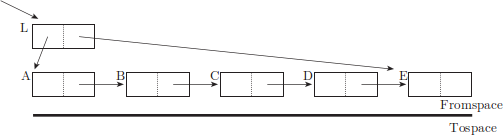
\includegraphics{figures/cop_1a}
    \caption{Ο χώρος-προς πριν τη συλλογή}
  \end{subfigure}

  \begin{subfigure}[b]{1.0\textwidth}
    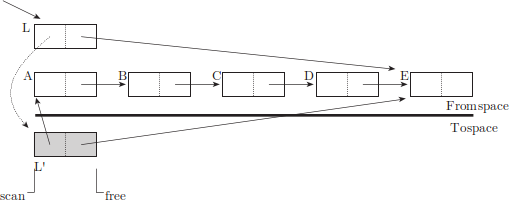
\includegraphics{figures/cop_1b}
    \caption{Αντιγραφή της ρίζας, $L$}
  \end{subfigure}
  
  \begin{subfigure}[b]{1.0\textwidth}
    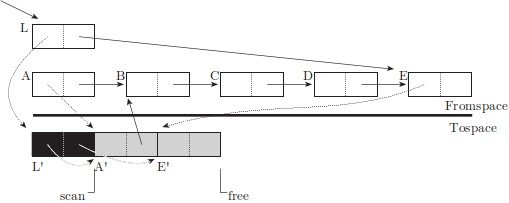
\includegraphics{figures/cop_1c}
    \caption{Σάρωση του αντιγράφου του $L$}
  \end{subfigure}
  \caption{Συλλογή με αντιγραφή: ένα παράδειγμα}
  \label{fig:cop_1}
\end{figure}

\begin{figure}[H]
  \ContinuedFloat
  \centering
  \begin{subfigure}{1.0\textwidth}
    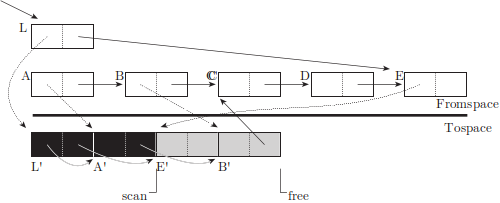
\includegraphics{figures/cop_2a}
    \caption{Σάρωση αντιγράφου του $Α$ κ.ο.κ}
  \end{subfigure}

  \begin{subfigure}[b]{1.0\textwidth}
    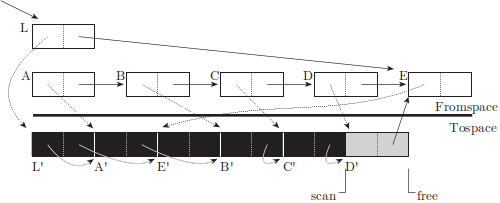
\includegraphics{figures/cop_2b}
    \caption{Σάρωση αντιγράφου του $C$}
  \end{subfigure}
  
  \begin{subfigure}[b]{1.0\textwidth}
    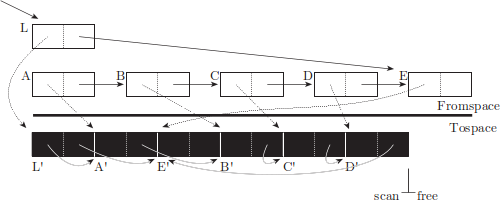
\includegraphics{figures/cop_2c}
    \caption{Σάρωση αντιγράφου του $D$. $scan=free$ και η 
             συλλογή ολοκληρώνεται.}
  \end{subfigure}
  \caption{Συλλογή με αντιγραφή: ένα παράδειγμα (συνέχεια)}
  \label{fig:cop_2}
\end{figure}

O White \cite{DBLP:conf/lfp/White80} ήταν ο πρώτος που συνέστησε τη χρήση του συλλέκτη
προς βελτίωση της επίδοσης του τροποποιητή. Τόσο η συλλογή με
αντιγραφή όσο και η συλλογή με σήμανση και συμπύκνωση μετακινούν
αντικείμενα, επηρεάζοντας με μεγάλη πιθανότητα την τοπικότητα
του τροποποιητή. Η ολισθαίνουσα μετακίνηση θεωρείται η βέλτιστη
όσον αφορά τη συλλογή με σήμανση και συμπύκνωση καθώς διατηρεί
τη διάταξη των αντικειμένων που έχει εγκαθιδρύσει ο εκχωρητής.
Η συντηρητική αυτή πολιτική είναι σίγουρα ασφαλής. Είναι όμως
και βέλτιστη; Η συλλογή με σήμανση και συμπύκνωση, η οποία 
συμπυκνώνει το σωρό επιτόπου είτε μετακινώντας ζωντανά αντικείμενα 
σε τρύπες είτε ολισθαίνοντας τα στο ένα άκρο του σωρού, δεν
έχει πολλές δυνατότητες τροποποίησης της διάταξης των αντικειμένων 
στο σωρό προς όφελος της τοπικότητας του τροποποιητή. Από την
άλλη πλευρά, οποιοσδήποτε αλγόριθμος συλλογής ο οποίος μετακινεί 
αντικείμενα σε μία φρέσκια περιοχή του σωρού χωρίς να καταστρέφει
τα αυθεντικά δεδομένα μπορεί να τα αναδιατάξει προκειμένου να
βελτιώσει την επίδοση του τροποποιητή.

Δυστυχώς υπάρχουν δύο λόγοι για τους οποίους δεν μπορούμε να
βρούμε μία βέλτιστη διάταξη των αντικειμένων που να ελαχιστοποιεί
τον αριθμό αστοχιών κρυφής μνήμης του προγράμματος. Πρώτον, ο
συλλέκτης δεν μπορεί να γνωρίζει το μοτίβο πρόσβασης των μελλοντικών
προσβάσεων σε αντικείμενα. Ακόμη χειρότερα, οι Petrank και Rawitz
\cite{DBLP:conf/popl/PetrankR02} αποδεικνύουν πώς το πρόβλημα της τοποθέτησης είναι NP-complete:
δεδομένης της τέλειας γνώσης των μελλοντικών προσβάσεων, δεν
υπάρχει αποδοτικός αλγόριθμος υπολογισμού μιας βέλτιστης τοποθέτησης.

\begin{algorithm}
  \caption{Σχεδόν κατά-βάθος αντιγραφή (Moon)}
  \label{alg:c_4}
  \begin{algorithmic}[1]
    \Procedure{initialize}{$worklist$}
      \State $scan \gets free$
      \State $partialScan \gets free$
    \EndProcedure
    \Statex
    \Procedure{isEmpty}{$worklist$}
      \State \Return{$scan=free$} \Comment{as per Cheney}
    \EndProcedure
    \Statex
    \Procedure{remove}{$worklist$}
      \If{$partialScan < free$}
        \State $ref \gets partialScan$ \Comment{prefer secondary scan}
        \State $partialScan \gets partialScan$ $+$ \Call{size}{$partialScan$}
      \Else
        \State $ref \gets scan$ \Comment{primary scan}
        \State $scan \gets scan$ $+$ \Call{size}{$scan$}
      \EndIf
      \State \Return{$ref$}
    \EndProcedure
    \Statex
    \Procedure{add}{$worklist$, $ref$} \Comment{secondary scan on the most recently allocated page}
      \State $partialScan \gets$ \Call{max}{$partialScan$, $startOfPage(ref)$}
    \EndProcedure
  \end{algorithmic}
\end{algorithm}

Η μοναδική λύση στο πρόβλημα είναι η χρήση ευριστικών. Μια πιθανή
προσέγγιση είναι η χρήση της συμπεριφοράς του παρελθόντος για την
πρόβλεψη της συμπεριφοράς του μέλλοντος. Ορισμένοι ερευνητές 
χρησιμοποιούν είτε στατιστική ανάλυση (profiling) βασιζόμενοι στην υπόθεση
των Calder κ.ά. \cite{DBLP:conf/asplos/CalderKJA98} πώς τα προγράμματα συμπεριφέρονται παρόμοια
για διαφορετικές εισόδους, είτε online δειγματοληψία (online sampling)
βασιζόμενοι στην υπόθεση των Chilimbi κ.ά. \cite{DBLP:conf/pldi/ChilimbiHL99}
πώς η συμπεριφορά του προγράμματος παραμένει η ίδια από μία
περίοδο στην επόμενη. Μια άλλη ευριστική είναι η διατήρηση της
διάταξης εκχώρησης, όπως κάνει η ολισθαίνουσα συμπύκνωση. Μια
τρίτη στρατηγική αφορά την προσπάθεια τοποθέτησης παιδιών δίπλα
σε έναν από τους γονείς τους, αφού ο μόνος τρόπος πρόσβασης ενός
παιδιού είναι η φόρτωση μιας αναφοράς από κάποιον από τους γονείς
αυτού. Ο αλγόριθμος του Cheney υλοποιεί κατά πλάτος αντιγραφή
τείνοντας όμως να τοποθετεί κοντά μακρινά ξαδέρφια και όχι γονείς
με τα παιδιά τους.

Οι αρχικές μελέτες του πώς μπορεί να επωφεληθεί η τοπικότητα
του τροποποιητή από τη σειρά αντιγραφής των αντικειμένων επικεντρώνονται
στην ελαχιστοποίηση των σφαλμάτων σελίδας: ο απώτερος στόχος 
είναι η τοποθέτηση σχετιζόμενων αντικειμένων στην ίδια σελίδα.
Οι Stamos \cite{stamos1982large, DBLP:journals/tocs/Stamos84}
και Blau \cite{DBLP:journals/pe/Blau83} διαπιστώνουν μέσω προσομοιώσεων
πώς παρότι η κατά βάθος αντιγραφή είναι πιο επικερδής από την
κατά πλάτος αντιγραφή, αυτή οδηγεί σε χειρότερη συμπεριφορά όσον
αφορά τα σφάλματα σελίδων σε σχέση με την αρχική διάταξη δημιουργίας
των αντικειμένων. Ο Wilson κ.ά. \cite{DBLP:conf/pldi/WilsonLM91}
ωστόσο υποστηρίζουν πώς οι εν λόγω προσομοιώσεις δε λαμβάνουν
υπόψη τους την τοπολογία των πραγματικών προγραμμάτων των γλωσσών
Lisp και Smalltalk, τα οποία τείνουν να δημιουργούν δένδρα με
μεγάλο πλάτος και μικρό βάθος: οι δενδρικές δομές υλοποιούν
πίνακες κατακερματισμού και έχουν σχεδιασθεί με στόχο την καλύτερη
διασπορά των κλειδιών προς αποφυγή συγκρούσεων.

Ο αλγόριθμος των Fenichel και Yochelson υλοποιεί την κατά βάθος
διάσχιση με τη χρήση μιας βοηθητικής στοίβας. Είναι πάντως δυνατή
η επίτευξη μιας σχεδόν κατά πλάτος διάσχισης χωρίς τη χρήση
βοηθητικής στοίβας. Ο Moon \cite{DBLP:conf/lfp/Moon84} τροποποίησε
τον αλγόριθμο του Cheney για να πετύχει μία σχεδόν κατά βάθος
διάσχιση. Ο αλγόριθμος του Moon χρησιμοποιεί εκτός του αρχικού
δείκτη $scan$ έναν επιπλέον δείκτη, τον $partialScan$. Οποτεδήποτε
αντιγράφεται ένα αντικείμενο, ο αλγόριθμος του Moon εκκινεί μια
δευτερεύουσα σάρωση στην τελευταία σελίδα του χώρου-προς η οποία
δεν έχει ακόμη σαρωθεί πλήρως. Όταν αυτό συμβεί, η κύρια σάρωση
συνεχίζει από την πρώτη σελίδα που δεν έχει σαρωθεί πλήρως. Στην
πράξη, η λίστα εργασιών υλοποιείται ως ένα ζεύγος ουρών Cheney.
Αυτή η \textbf{ιεραρχική αποσύνθεση} πλεονεκτεί έναντι της κλασσικής
κατά βάθος εξερεύνησης όσον αφορά την τοποθέτηση γονέων και
παιδιών στην ίδια σελίδα.

Το μειονέκτημα του αλγορίθμου του Moon είναι πώς αντικείμενα
μπορεί να σαρώνονται δύο φορές, αφού αυτός καταγράφει μόνο ένα
ζεύγος δεικτών σάρωσης και κατά συνέπεια ξεχνά τα μπλοκ μεταξύ
των θέσεων $scan$ και $free$ που έχουν ήδη μερικώς σαρωθεί.
Πράγματι, όπως διαπίστωσαν o Wilson κ.ά. \cite{DBLP:conf/pldi/WilsonLM91}
το 30\% των αντικειμένων ενδέχεται να σαρωθεί εις διπλούν. Οι
τελευταίοι τροποποίησαν τον αλγόριθμο του Moon παρέχοντας σε
κάθε σελίδα τους δικούς της δείκτες $free$ και $scan$, με τη
λίστα εργασιών να περιλαμβάνει πλέον τα μπλοκ που έχουν σαρωθεί
μερικώς. Αυτό σημαίνει πώς η κύρια σάρωση δεν χρειάζεται να
επισκεφθεί ξανά αντικείμενα σελίδων που έχει ήδη επεξεργασθεί
η δευτερεύουσα σάρωση.

\begin{figure}
  \centering
  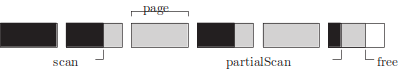
\includegraphics{figures/cop_4}
  \caption[Προσεγγιστική αντιγραφή κατά βάθος (Moon)]
   {Προσεγγιστική αντιγραφή κατά βάθος (Moon). Κάθε μπλοκ αναπαριστά
    μια σελίδα. Ως συνήθως, τα σαρωμένα πεδία είναι μαύρα, ενώ
    τα πεδία που έχουν αντιγραφεί αλλά όχι σαρωθεί ακόμη γκρι.
    Ο ελεύθερος χώρος απεικονίζεται με λευκό χρώμα.}
  \label{fig:cop_4}
\end{figure}

Η προσέγγιση του Moon είναι στατική και δε λαμβάνει υπόψη τη
συμπεριφορά των ξεχωριστών εφαρμογών. Είναι εμφανές ωστόσο πώς
τα οφέλη από την αναδιάταξη των αντικειμένων εξαρτώνται από τη
συμπεριφορά του τροποποιητή. Ο Lam κ.ά. \cite{DBLP:conf/iwmm/LamWM92}
διαπίστωσαν πώς ο αλγόριθμος του Moon παρουσιάζει ευαισθησία
όσον αφορά τη δομή και την ποικιλία των διαφόρων δομών δεδομένων
και εμφανίζει απογοητευτικές επιδόσεις για μη δενδροειδείς
δομές. Οι Siegwart και Hirzel \cite{DBLP:conf/iwmm/SiegwartH06}
επίσης παρατήρησαν πώς ένας παράλληλος συλλέκτης με ιεραρχική
αποσύνθεση ωφελεί σημαντικά την επίδοση μόνο ορισμένων benchmarks.

O Huang κ.ά. \cite{DBLP:conf/oopsla/HuangBMMWC04} παρακολουθούν
δυναμικά το προφίλ μιας εφαρμογής και προσπαθούν να αντιγράψουν
'θερμά' πεδία αντικειμένων δίπλα με τους γονείς αυτών. Αυτό το
σχήμα \textbf{online επαναδιάταξης αντικειμένων} καθώς και η
λειτουργία του φαίνονται στον αλγόριθμο~\ref{alg:cop_5} και το
σχήμα~\ref{fig:cop_3} αντίστοιχα. Ο βασικός βρόχος σάρωσης του
αλγορίθμου επεξεργάζεται πρώτα τη λίστα 'θερμών' αντικειμένων
και μετά τη λίστα ψυχρών αντικειμένων. Η υλοποίηση του μηχανισμού
δειγματοληψίας ως τμήμα ενός προσαρμοστικού δυναμικού μεταγλωττιστή
επιτρέπει τη φθηνή ταυτοποίηση των 'θερμών' αντικειμένων. Η υλοποίηση
των Huang κ.ά. επίσης λαμβάνει υπόψη τις αλλαγές της συμπεριφοράς
του τροποποιητή ανάμεσα στις διάφορες φάσεις λειτουργίας του,
επιτρέποντας στη 'θερμότητα' των πεδίων να φθίνει και να δειγματοληφθεί
ξανά. Τέλος, ο Huang κ.ά. διαπίστωσαν πώς η τεχνική της αντιγραφής
με online αναδιάταξη αντικειμένων εμφανίζει συγκρίσιμες ή και
καλύτερες επιδόσεις από στατικές τεχνικές όπως η αντιγραφή κατά
πλάτος.

\begin{algorithm}
  \caption{Online αναδιάταξη αντικειμένων}
  \label{alg:cop_5}
  \begin{algorithmic}[1]
    \Procedure{collect}{\null}
      \State \textbf{atomic}
      \State \Call{flip}{\null}
      \State \Call{initialize}{$hotList$, $coldList$}
      \ForAll{$fld \; \textbf{in} \; Roots$}
        \State \Call{adviceProcess}{$fld$}
      \EndFor
      \Repeat
        \While{\textbf{not} \Call{isEmpty}{$hotList$}}
          \State \Call{adviceScan}{$remove(hotList)$}
        \EndWhile
        \While{\textbf{not} \Call{isEmpty}{$coldList$}}
          \State \Call{adviceProcess}{$remove(coldList)$}
        \EndWhile
      \Until {\Call{isEmpty}{$hotList$}}
    \EndProcedure
    \Statex
    \Procedure{initialize}{$hotList$, $coldList$}
      \State $hotList \gets empty$
      \State $coldList \gets empty$
    \EndProcedure
    \Statex
    \Procedure{adviceProcess}{$fld$}
      \State $fromRef \gets *fld$
      \If{$fromRef \neq \textbf{null}$}
        \State $*fld \gets$ \Call{forward}{$fromRef$}
      \EndIf
    \EndProcedure
    \Statex
    \Procedure{adviceScan}{$obj$}
      \ForAll{$fld \; \textbf{in} \; Pointers(obj)$}
        \If{\Call{isHot}{$fld$}}
          \State \Call{adviceProcess}{$fld$}
        \Else
          \State \Call{add}{$coldList$, $fld$}
        \EndIf
      \EndFor
    \EndProcedure
  \end{algorithmic}
\end{algorithm}

\begin{figure}
  \centering
  \begin{subfigure}{1.0\textwidth}
    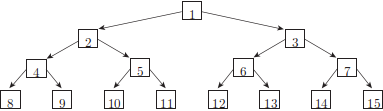
\includegraphics{figures/cop_3a}
    \caption{Το δένδρο προς αντιγραφή}
  \end{subfigure}

  \begin{subfigure}[b]{1.0\textwidth}
    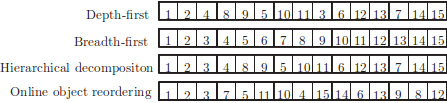
\includegraphics{figures/cop_3b}
    \caption{Τοποθέτηση αντικειμένων στο σωρό μετά την αντιγραφή}
  \end{subfigure}
  \caption[Αντιγραφή ενός δένδρου με διαφορετικές σειρές διάσχισης]
    {Αντιγραφή ενός δένδρου με διαφορετικές σειρές διάσχισης.
     Κάθε γραμμή δείχνει πώς η αντίστοιχη σειρά διάσχισης τοποθετεί
     τα αντικείμενα στο χώρο-προς, υποθέτοντας πώς κάθε σελίδα
     χωράει τρία αντικείμενα.}
  \label{fig:cop_3}
\end{figure}

\section{Θέματα προς εξέταση}
\subsection{Εκχώρηση μνήμης}
Η εκχώρηση μνήμης σε έναν συμπυκνωμένο σωρό είναι γρήγορη επειδή
είναι απλή. Συνήθως απλώς απαιτεί τον έλεγχο έναντι ενός άνω 
ορίου (του σωρού ή ενός μπλοκ) και την υλοποίηση ενός δείκτη 
$free$. Εάν ο σωρός είναι οργανωμένος σε μπλοκ και όχι συνεχόμενος,
ο έλεγχος ενίοτε θα αποτυγχάνει στην οποία περίπτωση πρέπει να
δεσμευθεί ένα καινούριο μπλοκ. Η συχνότητα εμφάνισης της αργής
αυτής περίπτωσης θα εξαρτηθεί από το πώς μεταβάλλεται ο μέσος 
όρος μεγέθους των δημιουργούμενων αντικειμένων και το μέγεθος 
του μπλοκ. Η σειριακή εκχώρηση μνήμης επίσης είναι κατάλληλη
για χρήση σε πολυνηματικές εφαρμογές, καθώς σε κάθε νήμα τροποποιητή
μπορεί να δοθεί ένας τοπικός απομονωτής εκχώρησης χωρίς να
χρειάζεται ο συγχρονισμός με άλλα νήματα. Η οργάνωση αυτή είναι
απλή και απαιτεί τη χρήση μικρού αριθμού μεταδεδομένων, σε αντίθεση
με τοπικά σχήματα εκχώρησης για μη μετακινούντες συλλέκτες όπου
κάθε νήμα τροποποιητής μπορεί να χρειάζεται τις δικές του δομές
δεδομένων για την εκχώρηση μνήμης με ξεχωριστές ελεύθερες λίστες 
για αντικείμενα διαφορετικού μεγέθους.

Ο κώδικας που υλοποιεί τη σειριακή εκχώρηση είναι σύντομος 
και επιπλέον παρουσιάζει καλή συμπεριφορά όσον αφορά την κρυφή
μνήμη καθώς η εκχώρηση προχωράει σειριακά στο σωρό. Παρότι ο
συνδυασμός της σειριακής εκχώρησης, της μικρής διάρκειας ζωής
αντικειμένων και της οργάνωσης του σωρού σε ημιχώρους συνεπάγεται
πώς με μεγάλη πιθανότητα η επόμενη θέση μνήμης που θα εκχωρηθεί
είναι αυτή που έχει χρησιμοποιηθεί λιγότερο πρόσφατα, οι μηχανισμοί
προφόρτωσης των σύγχρονων επεξεργαστών συνήθως καλύπτουν την
λανθάνουσα καθυστέρηση που προκύπτει. Εάν όμως η συμπεριφορά
αυτή συγκρούεται με την πολιτική αντικατάστασης της λιγότερο 
πρόσφατα χρησιμοποιημένης σελίδας (LRU) του λειτουργικού
συστήματος σε βαθμό ώστε ο ρυθμός εναλλαγής σελίδων να χειροτερεύει
την επίδοση, τότε χρειάζεται επανεξέταση της διαμόρφωσης του
συστήματος διαχείρισης μνήμης. Η ικανοποιητική εκτέλεση της
εφαρμογής μπορεί να απαιτεί περισσότερη φυσική μνήμη ή αλλαγή
της πολιτικής συλλογής.

Ο Blackburn κ.ά. \cite{DBLP:conf/icse/BlackburnCM04} κατά την πειραματική μελέτη ενός
μικρού σχετικά benchmark διαπίστωσαν πώς παρότι η σειριακή
εκχώρηση υπερτερεί κατά 11\% έναντι της εκχώρησης με ελεύθερες
λίστες, η εκχώρηση καθεαυτή αποτελεί μόλις το 10\% του
συνολικού χρόνου εκτέλεσης μιας εφαρμογής. Επομένως η διαφορά
κόστους ανάμεσα στις δύο τεχνικές μπορεί να είναι αμελητέα.
Ωστόσο το κυρίαρχο κόστος της δημιουργίας ενός αντικειμένου 
συνήθως αφορά την αρχικοποίηση του αντικειμένου και όχι την
εκχώρηση μνήμης. Επιπλέον, τα αντικείμενα έχουν παρόμοιους
κύκλους ζωής σε πολλές εφαρμογές. Ο τροποποιητής δημιουργεί
έναν αριθμό από σημασιολογικά συνδεδεμένα αντικείμενα περίπου
την ίδια χρονική περίοδο, τα επεξεργάζεται και τα εγκαταλείπει
μαζικώς. Σε τέτοιες εφαρμογές η χρήση συμπυκνωμένου σωρού
προσφέρει υψηλή τοπική χωρικότητα αφού τα σχετιζόμενα αντικείμενα
τοποθετούνται στην ίδια σελίδα ή ακόμη και στο ίδιο μπλοκ
κρυφής μνήμης αν είναι μικρά. Μια τέτοια διάταξη τείνει
εμφανώς να οδηγήσει σε χαμηλότερο ρυθμό αστοχιών κρυφής
μνήμης σε σύγκριση με την περίπτωση όπου η μνήμη των συσχετιζόμενων
αντικειμένων εκχωρείται μέσω ξεχωριστών ελεύθερων λιστών.

\subsection{Χώρος και τοπικότητα}
Το άμεσο μειονέκτημα της συλλογής με αντιγραφή ημιχώρων είναι
η ανάγκη διατήρησης ενός δεύτερου ημιχώρου, ο οποίος μερικές
φορές καλείται και \textbf{εφεδρικό αντίγραφο (copy reserve)}.
Δεδομένου ενός προϋπολογισμού μνήμης και αγνοώντας τις δομές
δεδομένων που είναι απαραίτητες για τη λειτουργία του συλλέκτη
η συλλογή με αντιγραφή προσφέρει μόνο το μισό χώρο του σωρού
σε σχέση με άλλες τεχνικές συλλογής σκουπιδιών. Το αποτέλεσμα
είναι πώς οι συλλέκτες με αντιγραφή θα πραγματοποιήσουν περισσότερους
κύκλους συλλογής από ότι άλλοι συλλέκτες. Εάν αυτό θα οδηγήσει
σε καλύτερη ή χειρότερη επίδοση εξαρτάται από τους διάφορους
συμβιβασμούς μεταξύ συλλέκτη και τροποποιητή, τα χαρακτηριστικά
της εφαρμογής και το ποσό της διαθέσιμης μνήμης σωρού.

Η απλή ασυμπτωτική ανάλυση πολυπλοκότητας μπορεί να προτιμήσει
τη συλλογή με αντιγραφή έναντι της συλλογής με σήμανση και
εκκαθάριση. Έστω $M$ το συνολικό μέγεθος του σωρού και $L$ το
συνολικό μέγεθος των ζωντανών αντικειμένων. Η συλλογή με αντιγραφή
πρέπει να αντιγράψει και σαρώσει τα ζωντανά αντικείμενα καθώς
και να ενημερώσει τους δείκτες αυτών. Η συλλογή με σήμανση και
εκκαθάριση από την άλλη πλευρά πρέπει να ανακαλύψει όλα τα ζωντανά
αντικείμενα και στη συνέχεια να εκκαθαρίσει όλο το σωρό.
Ο Jones \cite{DBLP:books/wi/JonesL96} ορίζει τη χρονική πολυπλοκότητα για τη συλλογή
με αντιγραφή και για τη συλλογή με σήμανση και εκκαθάριση ως:

\begin{align}
t_{copy} &= cL \\
 t_{MS} &= mL+sM
\end{align}

Το ποσό της μνήμης που ανακτάται από κάθε συλλογή είναι αντίστοιχα:

\begin{align}
m_{copy} &= \frac{M}{2}-L \\
 m_{MS} &= M-L
\end{align}

Έστω τώρα $r=\frac{L}{M}$ το ποσοστό της ζωντανής μνήμης, το
οποίο υποθέτουμε πώς είναι σταθερό. Η αποδοτικότητα ενός αλγορίθμου
μπορεί να περιγραφεί από το λόγο mark/cons, $e$, ο οποίος αντιπροσωπεύει
την εργασία του συλλέκτη ανά μονάδα ανακτημένης μνήμης.

\begin{align}
e_{copy} &= \frac{2cr}{1-2r} \\
 e_{MS} &= \frac{mr+s}{1-r}
\end{align}

\begin{figure}
  \centering
  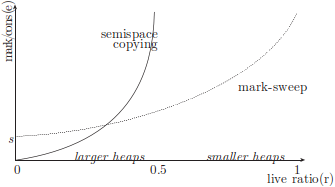
\includegraphics{figures/cop_5}
  \caption[Ρυθμοί mark/cons για συλλογή με σήμανση και εκκαθάριση
           και συλλογή με αντιγραφή.]
    {Ρυθμοί mark/cons για συλλογή με σήμανση και εκκαθάριση και
     συλλογή με αντιγραφή.}
  \label{fig:cop_5}
\end{figure}

Η συλλογή με αντιγραφή μπορεί να είναι πιο αποδοτική από τη
συλλογή με σήμανση και εκκαθάριση αν ο σωρός είναι αρκετά μεγάλος
και το $r$ αρκετά μικρό. Αυτή η απλουστευμένη ανάλυση ωστόσο
αγνοεί διάφορα ζητήματα. Οι σύγχρονοι συλλέκτες με σήμανση
και εκκαθάριση συνήθως χρησιμοποιούν οκνηρή εκκαθάριση, κάτι
που μειώνει τη σταθερά $s$ και κατ' επέκταση το λόγο $e_{MS}$.
Η ανάλυση της πολυπλοκότητας πρέπει να αντιμετωπισθεί με μεγάλη
προσοχή καθώς συνήθως αγνοεί λεπτομέρειες υλοποίησης παρότι
οι Hertz και Berger \cite{DBLP:conf/oopsla/HertzB05} επιβεβαιώνουν πειραματικά τη μορφή 
των καμπυλών (όπως ότι το κόστος της συλλογής με σήμανση και
εκκαθάριση είναι αντιστρόφως ανάλογο προς το μέγεθος του σωρού).
Οι πραγματικές λεπτομέρειες υλοποίησης παρότι είναι σημαντικές 
για πραγματικούς συλλέκτες δεν λαμβάνονται υπόψη από αναλύσεις
πολυπλοκότητας. Παράδειγμα μιας τέτοιας λεπτομέρειας αποτελεί
η θετική επίδραση στην τοπικότητα του τροποποιητή της χρήσης
σειριακής εκχώρησης μνήμης \cite{DBLP:conf/icse/BlackburnCM04}.

Επομένως η διαδοχική εκχώρηση μνήμης τείνει να τοποθετεί αντικείμενα
που προσπελάζονται ταυτόχρονα σε διαδοχικές θέσεις μνήμης, κάτι
που συμβάλλει στη βελτίωση του ρυθμού αστοχιών κρυφής μνήμης
του τροποποιητή. Ωστόσο η συλλογή με αντιγραφή αναδιατάσσει
τα επιζώντα αντικείμενα στο σωρό. Παρότι η συλλογή με αντιγραφή
κατά Cheney δεν χρειάζεται βοηθητική στοίβα για την καθοδήγηση
της εξιχνίασης, η διάσχιση κατά πλάτος τείνει να διαχωρίζει τους
γονείς από τα παιδιά τους. Η ιεραρχική αποσύνθεση προσφέρει
έναν καλό συμβιβασμό μεταξύ της πληρωμής του κόστους της βοηθητικής 
στοίβας και της βελτίωσης της διάταξης των αντικειμένων στο σωρό.
Ωστόσο παρότι η προσεκτική αναδιάταξη των αντικειμένων μπορεί
να είναι ωφέλιμη για μερικά προγράμματα, σε ορισμένες περιπτώσεις
η επίδρασή της μπορεί να αποδειχθεί αμελητέα. Τα περισσότερα
αντικείμενα έχουν μικρή διάρκεια ζωής και δεν επιβιώνουν ούτε
μία συλλογή. Επιπλέον, όπως παρατηρούν οι Blackburn και McKinley
\cite{DBLP:conf/oopsla/BlackburnM03}, πολλές εφαρμογές εστιάζουν τις προσβάσεις στη μνήμη και
ιδιαίτερα τις εγγραφές σε αυτά τα νέα αντικείμενα. Η πολιτική
διάσχισης ενός συλλέκτη δεν μπορεί προφανώς να επηρεάσει την
ιδιότητες τοπικότητας αντικειμένων που δεν μετακινούνται.

\subsection{Μετακίνηση αντικειμένων}
Η επιλογή ενός συλλέκτη αντιγραφής εξαρτάται μεταξύ άλλων από το
αν επιτρέπεται η μετακίνηση αντικειμένων καθώς από το κόστος της
μετακίνησης. Σε μερικά περιβάλλοντα δεν επιτρέπεται η μετακίνηση
αντικειμένων. Ένας από τους λόγους είναι η έλλειψη πληροφορίας
τύπων που καθιστά μη ασφαλή την τροποποίηση ενός πεδίου που είναι
πιθανόν δείκτης σε ένα αντικείμενο. Ένας διαφορετικός λόγος είναι
πώς μπορεί μια αναφορά προς ένα αντικείμενο να έχει μεταβιβασθεί 
ως σε μη διαχειρίσιμο κώδικα (για παράδειγμα ως όρισμα σε κάποια
κλήση συστήματος). Επιπλέον το πρόβλημα της εύρεσης δεικτών πολύ
συχνά είναι απλούστερο συλλογή με σήμανση και εκκαθάριση από ότι
στη συλλογή με αντιγραφή. Αρκεί η ανακάλυψη τουλάχιστον μιας
αναφοράς προς ένα ζωντανό αντικείμενο όταν χρησιμοποιείται ένας
μη μετακινών συλλέκτης. Από την άλλη πλευρά, ένας μετακινών
συλλέκτης πρέπει να εντοπίσει και ενημερώσει όλες τις αναφορές
προς ένα μετακινηθέν αντικείμενο. Όπως θα δούμε και στο κεφάλαιο
\ref{ch:conc}, το γεγονός αυτό καθιστά την ταυτόχρονη συλλογή
με μετακίνηση σημαντικά δυσκολότερη από την ταυτόχρονη συλλογή 
χωρίς μετακίνηση καθώς όλες οι ενημερώσεις των αναφορών προς
κάθε αντικείμενο πρέπει να εμφανίζονται ως ατομικές.

Η αντιγραφή ορισμένων αντικειμένων είναι ακριβή. Παρότι η
αντιγραφή ενός μικρού αντικειμένου κοστίζει περισσότερο από
τη σήμανση αυτού, το κόστος και η λανθάνουσα καθυστέρηση της
αντιγραφής συχνά κρύβονται από το κόστος της παρακολούθησης
δεικτών και της ανακάλυψης πληροφορίας τύπων. Από την άλλη
πλευρά η επαναλαμβανόμενη αντιγραφή μεγάλων αντικειμένων μπορεί
να οδηγήσει σε φτωχές επιδόσεις. Μια λύση είναι η αποφυγή
της αντιγραφής τους και η ανάθεση της διαχείρισής τους σε
έναν μη μετακινούντα συλλέκτη. Μια άλλη λύση είναι η αντιγραφή
τους να πραγματοποιείται εικονικά και όχι φυσικά.

\end{greek}

\begin{greek}
\chapter{Συλλογή σκουπιδιών με καταμέτρηση αναφορών}\label{ch:refcnt}
Οι αλγόριθμοι που έχουμε εξετάσει μέχρι στιγμής είναι έμμεσοι:
κάθε ένας από αυτούς διασχίζει τον γράφο των αντικειμένων
ώστε να αναγνωρίσει τα ζωντανά αντικείμενα. Σε αυτό το κεφάλαιο
εξετάζουμε την τέταρτη και τελευταία θεμελιώδη τεχνική συλλογής
σκουπιδιών, αυτήν της καταμέτρησης αναφορών.  
Η \textbf{συλλογή σκουπιδιών με καταμέτρηση αναφορών}, η
οποία οφείλεται στον Collins \cite{DBLP:journals/cacm/Collins60},
δεν επισκέπτεται όλο το σωρό προκειμένου να εντοπίσει τα
ζωντανά αντικείμενα και να συμπεράνει πώς όλα τα υπόλοιπα
είναι σκουπίδια, αλλά επιδρά απευθείας στα αντικείμενα
καθώς αναφορές σε αυτά δημιουργούνται ή καταστρέφονται.

Η αλγόριθμος διατηρεί μια απλή αναλλοίωτη: ένα αντικείμενο
θεωρείται ζωντανό αν και μόνο αν ο αριθμός των αναφορών σε
αυτό είναι αυστηρά θετικός. Η συλλογή με καταμέτρηση αναφορών
συσχετίζει λοιπόν έναν μετρητή αναφορών με κάθε διαχειριζόμενο
αντικείμενο. Ο μετρητής αυτός συνήθως αποθηκεύεται σε ένα
πεδίο στην  επικεφαλίδα του αντικειμένου.

Ο αλγόριθμος \ref{alg:refcnt_1} αποτελεί την απλούστερη
εκδοχή της συλλογής με καταμέτρηση αναφορών. Η διαδικασία
\textproc{Write} αυξάνει το μετρητή αναφορών του νέου
αντικειμένου στο οποίο αναφέρεται ένας δείκτης και μειώνει
το μετρητή αναφορών του παλαιού αντικειμένου προς το οποίο
αυτός αναφερόταν. Η διαδικασία αυτή καλείται ακόμη και για
την ενημέρωση τοπικών μεταβλητών. Κατά την έξοδο μιας
διαδικασίας, τέλος, η \textproc{Write} καλείται για να
ενημερώσει με την τιμή \null τις τοπικές μεταβλητές αυτής.
Οι διαδικασίες \textproc{addReference} και \textproc{deleteReference}
αυξάνουν και μειώνουν αντίστοιχα το μετρητή αναφορών του
αντικειμένου όρισματός τους. Μόλις ένας μετρητής αναφορών
ενός αντικειμένου μηδενισθεί, τότε πριν η μνήμη αυτού
απελευθερωθεί, μειώνονται κατά ένα οι μετρητές αναφορών
των αντικειμένων στα οποία δείχνουν τα πεδία δείκτες
του.

Η μέθοδος \textbf{Write} αποτελεί ένα παράδειγμα ενός φράγματος
εγγραφής. Για κάθε φράγμα εγγραφής, ο μεταγλωττιστής παράγει
μία ακολουθία κώδικα πριν και μετά την εγγραφή ενός δείκτη.
Όπως θα δούμε και αργότερα, τα φράγματα εγγραφής είναι
απαραίτητα στην περίπτωση που οι συλλέκτες δε θεωρούν τη
ζωντάνια ολόκληρου του γράφου αντικειμένων ατομικά ως προς
τον τροποποιητή. Οι ταυτόχρονοι καθώς και οι γενεαλογικοί
συλλέκτες αποτελούν παραδείγματα τέτοιων συλλεκτών. Σε κάθε
περίπτωση, τα φράγματα εγγραφής εγγυώνται τη διατήρηση της
αναλλόιωτης του εκάστοτε αλγορίθμου συλλογής.

\begin{algorithm}[H]
  \caption{Απλή καταμέτρηση αναφορών}
  \label{alg:refcnt_1}
  \begin{algorithmic}[1]
    \Function{New}{\null}
      \State $ref \gets$ \Call{allocate}{\null}
      \If{$ref = \textbf{null}$}
        \State error ``Out of memory!''
      \EndIf
      \State \Call{rc}{$ref$} $\gets 0$
      \State \Return{$ref$}
    \EndFunction
    \Statex
    \Procedure{write}{$src$, $i$, $ref$}
      \State \textbf{atomic}
      \State \Call{addReference}{$ref$}
      \State \Call{deleteReference}{$src[i]$}
      \State $src[i] \gets ref$
    \EndProcedure
    \Statex
    \Procedure{addReference}{$ref$}
      \If{$ref \neq \textbf{null}$}
        \State \Call{rc}{$ref$} $\gets$ \Call{rc}{$ref$} $+1$
      \EndIf
    \EndProcedure
    \Statex
    \Procedure{deleteReference}{$ref$}
      \If{$ref \neq \textbf{null}$}
        \State \Call{rc}{$ref$} $\gets$ \Call{rc}{$ref$} $-1$
        \If{\Call{rc}{$ref$} $=$ $0$}
          \ForAll{$fld \; \textbf{in} Pointers(ref)$}
            \State \Call{deleteReference}{$*fld$}
          \EndFor
          \State \Call{free}{$ref$}
        \EndIf
      \EndIf
    \EndProcedure
  \end{algorithmic}
\end{algorithm}

\section{Πλεονεκτήματα \& Μειονεκτήματα}
Υπάρχουν αρκετοί λόγοι για τους οποίους η συλλογή με καταμέτρηση
αναφορών αποτελεί ελκυστική επιλογή. Αρχικά, το κόστος της
διαχείρισης μνήμης κατανέμεται στις λειτουργίες εγγραφής του
τροποποιητή, χωρίς να απαιτείται η παύση της εκτέλεσης αυτού.
Η μνήμη ενός αντικειμένου απελευθερώνεται αμέσως μόλις δεν
υπάρχει καμία αναφορά προς αυτό, κάτι που καθιστά τον αλγόριθμο
κατάλληλο για λειτουργία σε εφαρμογές όπου ο σωρός είναι
σχεδόν γεμάτος. Αντίθετα, οι συλλέκτες με εξιχνίαση, χρειάζονται
κάποιο χώρο στο σωρό ώστε να λειτουργήσουν. Επιπρόσθετα,
καθώς η καταμέτρηση αναφορών επιδρά απευθείας στα αντικείμενα
προέλευσης και προορισμού των δεικτών, η τοπικότητα του συλλέκτη
δε μπορεί να είναι χειρότερη από την τοπικότητα του τροποποιητή.
Ακόμη η συλλογή με καταμέτρηση αναφορών μπορεί να υλοποιηθεί
χωρίς καμία βοήθεια από το σύστημα εκτέλεσης ή το μεταγλωττιστή,
καθώς δεν απαιτεί τη γνώση των ριζών του προγράμματος. Τέλος,
όπως παρατηρούν οι Rodrigues και Jones \cite{DBLP:conf/wdag/RodriguesJ96}
η καταμέτρηση αναφορών μπορεί να ανακτήσει μνήμη ακόμα και
αν κάποια του συστήματος δεν είναι προσβάσιμα, κάτι που έχει
μεγάλη σημασία σε κατανεμημένα συστήματα.

Για όλους τους παραπάνω λόγους, η συλλογή με καταμέτρηση
αναφορών έχει υιοθετηθεί από πολλά συστήματα λογισμικού,
ανάμεσα στα οποία περιλαμβάνονται: υλοποιήσεις γλωσσών
προγραμματισμού (αρχικές εκδόσεις Smalltalk και Lisp, awk,
perl, python), εφαρμογές όπως το Photoshop, συστήματα
διαχείρισης εγγράφων και συστήματα διαχείρισης αρχείων
λειτουργικών συστημάτων. Επίσης, βιβλιοθήκες για ασφαλή
ανάκτηση μνήμης αντικειμένων είναι διαθέσιμες για γλώσσες
των οποίων το πρότυπο δεν επιβάλλει (ακόμη) αυτόματη
διαχείριση μνήμης. Οι βιβλιοθήκες αυτές χρησιμοποιούν
έξυπνους δείκτες για την πρόσβαση σε αντικείμενα. Οι
έξυπνοι δείκτες υπερφορτώνουν κατασκευαστές και τελεστές
όπως η ανάθεση, είτε για να επιβάλλουν αποκλειστική ιδιοκτησία
στα αντικείμενα είτε για να παρέχουν καταμέτρηση αναφορών.
Ο Edelson \cite{DBLP:conf/iwmm/Edelson92} ωστόσο παρατηρεί
πώς οι έξυπνοι δείκτες έχουν διαφορετική σημασιολογία από
τους "πρωτόγονους" δείκτες που προσπαθούν να μοντελοποιήσουν.

Ωστόσο, τη συλλογή σκουπιδιών με καταμέτρηση αναφορών
χαρακτηρίζουν και διάφορα μειονεκτήματα.

Πρώτον, η καταμέτρηση αναφορών επιβάλλει ένα χρονικό κόστος
στον τροποποιητή. Σε αντίθεση με τους αλγορίθμους εξιχνίασης
που εξετάσαμε στα προηγούμενα κεφάλαια, η κατάμετρηση αναφορών
επανορίζει όλες τις λειτουργίες \textproc{Read} και
\textproc{Write} δεικτών προκειμένου να διαχειστεί τους
μετρητές αναφορών. Ακόμη και μια απλή διάσχιση μιας λίστας
απαιτεί μία αύξηση και μία μείωση ενός μετρητή αναφοράς για
κάθε αντικείμενο αυτής. Από άποψη επίδοσης, η επιβάρυνση
λειτουργιών που ενημερώνουν καταχωρητές και κομμάτια της
στοίβας είναι απαγορευτική. Γι αυτόν ακριβώς το λόγο, ο
απλοϊκός αλγόριθμος που παρουσιάστηκε είναι πρακτικά μη
εφαρμόσιμος για χρήση σε ένα γενικού σκοπού υψηλών επιδόσεων
διαχειριστή μνήμης.

Δεύτερον, τόσο οι ενέργεις που αφορούν διαχείριση των μετρητών
αναφορών όσο και οι φορτώσεις και αποθηκεύσεις δεικτών πρέπει
να είναι ατομικές ώστε να αποφευχθούν καταστάσεις συναγωνισμού
μεταξύ των νημάτων του τροποποιητή οι οποίες θα μπορούσαν να
οδηγήσουν σε πρώιμη αποδέσμευση της μνήμης ενός αντικειμένου.
Η εξασφάλιση της ατομικότητας μόνο της λειτουργίας ενημέρωσης
του μετρητή αναφοράς δεν επαρκεί. Κάποιες βιβλιοθήκες έξυπνων
δεικτών απαιτούν ιδιαίτερα προσεκτική μεταχείριση προκειμένου
να αποφευχθούν οι καταστάσεις συναγωνισμού. Για παράδειγμα,
η βιβλιοθήκη έξυπνων δεικτών Boost για τη γλώσσα C++, η οποία
παρέχει και λειτουργίες καταμέτρησης αναφορών, νήματα που
εκτελούνται ταυτόχρονα μπορεί είτε να διαβάζουν τον ίδιο
μοιραζόμενο δείκτη ταυτόχρονα είτε να μεταβάλλουν διαφορετικά
στιγμιότυπα αυτού. Η βιβλιοθήκη εξασφαλίζει όμως την
ατομικότητα μόνο των λειτουργιών αύξησης/μείωσης του μετρητή
αναφορών. Ο συνδυασμός ανάγνωσης/εγγραφής ενός δείκτη με την
ενημέρωση ενός μετρητή αναφοράς δεν αποτελεί μία μοναδική
ατομική πράξη.

Τρίτον, η απλοϊκή μέτρηση αναφορών μετατρέπει λειτουργίες
ανάγνωσης-μόνο (read-only) σε λειτουργίες που απαιτούν εγγραφή
στη μνήμη (ώστε να ενημερωθούν οι μετρητές αναφορών). Όμοια,
απαιτείται η ανάγνωση και εγγραφή του παλαιού αντικειμένου
αναφοράς ενός δείκτη πριν αυτός αλλάξει τιμή. Αυτές οι εγγραφές
"μολύνουν" τη μνήμη cache και επιφέρουν επιπλέον κίνηση μεταξύ
μνήμης και επεξεργαστή.

Τέταρτον, η συλλογή με καταμέτρηση αναφορών αδυνατεί να συλλέξει
κυκλικές δομές δεδομένων (δομές δεδομένων που περιλαμβάνουν
αναφορές στον εαυτό τους). Ακόμη και αν μία τέτοια δομή είναι
απομονωμένη στο γράφο των αντικειμένων (δεν υπάρχει δηλαδή
μονοπάτι προς αυτή από τις ρίζες), οι μετρητές αναφοράς των
συνιστωσών της δε θα μηδενισθούν ποτέ. Οι Bacon και Rajan
\cite{DBLP:conf/ecoop/BaconR01} διαπιστώνουν πώς αυτοαναφορικές
δομές (διπλά συνδεδεμένες λίστες, κυκλικές ουρές, δένδρα με
δείκτες προς τη ρίζα κ.ά) απαντώνται συχνά στις εφαρμογές,
παρότι η συχνότητά τους μπορεί να ποικίλλει σημαντικά από
εφαρμογή σε εφαρμογή.

Πέμπτον, στη χειρότερη περίπτωση, ο αριθμός των αναφορών σε
ένα αντικείμενο μπορεί να ισούται με το πλήθος των αντικειμένων
του σωρού. Αυτό συνεπάγεται πώς ο μετρητής αναφορών θα
καταλαμβάνει μια ολόκληρη λέξη μνήμης. Λαμβάνοντας υπόψη την
διαπίστωση των Dieckmann και H{\"o}lzle
\cite{DBLP:conf/ecoop/DieckmannH99} και Blackburn
κ.ά \cite{DBLP:conf/oopsla/BlackburnGHKMBDFFGHHJLMPSVDW06}
πώς το μέσο μέγεθος αντικειμένων στις αντικειμενοστραφείς
γλώσσες είναι μικρό (στη Java 20-64 bytes) καθώς το γεγονός
πώς τα κελιά cons στη Lisp χρειάζονται συνήθως 2-3 λέξεις,
η επιβάρυνση σε χώρο μπορεί να είναι σημαντική.

Τέλος, η συλλογή σκουπιδιών με καταμέτρηση αναφορών μπορεί
επίσης να προκαλέσει παύσεις. Τη στιγμή που διαγράφεται ο
δείκτης στην κεφαλή μιας μεγάλης δομής δεδομένων, η διαδικασία 
\textproc{deleteReference} θα πρέπει να ελευθερώσει αναδρομικά
τη μνήμη όλων των αντικειμένων απογόνων της ρίζας. Ο Boehm
\cite{DBLP:conf/popl/Boehm04} μάλιστα ισχυρίζεται πώς οι
παύσεις αυτές μπορεί ακόμα και να ξεπεράσουν τις αντίστοιχες
παύσεις από συλλέκτες εξιχνίασης.

Στη συνέχεια εξετάζουμε προηγμένους αλγορίθμους συλλογής
σκουπιδιών με καταμέτρηση αναφορών.

\section{Καταμέτρηση αναφορών με αναβολή}
Τα περισσότερα συστήματα υψηλών επιδόσεων με καταμέτρηση
αναφορών, όπως για παράδειγμα των Blackburn και McKinley
\cite{DBLP:conf/oopsla/BlackburnM03} χρησιμοποιούν την τεχνική
της \textbf{καταμέτρησης αναφορών με αναβολή}. Η συντριπτική
πλειοψηφία των φορτώσεων δεικτών αφορά τοπικές και προσωρινές
μεταβλητές, δηλαδή καταχωρητές και στοίβα. Οι Deutsch και
Bobrow \cite{DBLP:journals/cacm/DeutschB76} έδειξαν πώς μπορούν
να αποφευχθούν οι ενέργειες καταμέτρησης αναφορών που αφορούν
αυτές τις λειτουργίες, ενημερώνοντας το μετρητή ενός αντικειμένου
μόνο όταν ο δείκτης προς αυτό αποθηκεύεται στο πεδίο κάποιου
αντικειμένου του σωρού. Οι λειτουργίες καταμέτρησης αναφορών
που αφορούν καταχωρητές και τη στοίβα αναβάλλονται. Με την
τεχνική αυτή, οι μετρητές αναφορών των τοπικών μεταβλητών
παύουν να είναι αξιόπιστοι: δεν είναι πλέον ασφαλής η
αποδέσμευση ενός αντικειμένου αν ο μετρητής αναφορών του
είναι μηδενικός. Η ανακύκλωση των αντικειμένων σκουπιδιών
απαιτεί την περιοδική διόρθωση των μετρητών κατά τη διάρκεια
παύσεων. Ο Ungar \cite{DBLP:conf/sde/Ungar84} δείχνει πώς
οι παύσεις αυτές είναι σημαντικά μικρότερες σε σχέση με τις
αντίστοιχες ενός συλλέκτη με σήμανση και εκκαθάριση.

Ο αλγόριθμος~\ref{alg:refcnt_2} φορτώνει τις αναφορές σε
αντικείμενα χρησιμοποιώντας, την απλή, χωρίς φράγμα υλοποίηση
\textproc{Read} που ορίστηκε στο κεφάλαιο~\ref{ch:intro}.
Παρόμοια, οι ρίζες ενημερώνονται με αναφορές χρησιμοποιώντας
μία μη φραγμένη εντολή store. Αντίθετα, οι εγγραφές σε
αντικείμενα του σωρού πρέπει να είναι φραγμένες. Στην
περίπτωση αυτή, η αύξηση ενός μετρητή αναφοράς γίνεται
κανονικά ως συνήθως. Ωστόσο, αν η μείωση του μετρητή αναφορών
του αντικειμένου στο οποίο έδειχνε ένας δείκτης έχει ως
αποτέλεσμα το μηδενισμό του μετρητή, το φράγμα εγγραφής
\textproc{Write} προσθέτει το αντικείμενο (μια αναφορά σε
αυτό) σε ένα πίνακα μηδενικών μετρητών (μεταβλητή $zct$)
αντί να το απελευθερώσει αμέσως. Ο πίνακας αυτός μπορεί
να υλοποιηθεί με διαφόρους τρόπους, χρησιμοποιώντας ένα
bitmap όπως ο Baden \cite{baden1983low} ή ένα hashtable
όπως οι Deutsch και Bobrow \cite{DBLP:journals/cacm/DeutschB76}.
H ανακύκλωση ενός αντικειμένου με μηδενικό μετρητή αναφορών
σε αυτό το σημείο δεν είναι ασφαλής, καθώς ενδέχεται να
υπάρχει μια αναφορά σε αυτό από τη στοίβα του προγράμματος.
Διαισθητικά, ο πίνακας μηδενικών μετρητών περιλαμβάνει
αναφορές σε αντικείμενα με μηδενικό μετρητή αναφορών τα
οποία μπορεί όμως να είναι ζωντανά.

Ωστόσο, τα αντικείμενα σκουπίδια πρέπει κάποια στιγμή να
συλλεγούν αν θέλουμε το πρόγραμμα να μην ξεμείνει από μνήμη.
Περιοδικά, για παράδειγμα όταν ο εκχωρητής αποτύχει να
επιστρέψει μνήμη στη συνάρτηση \textproc{New}, διακόπτεται
η λειτουργία των νημάτων του τροποποιητή και τα αντικείμενα
του πίνακα μηδενικών μετρητών εξετάζονται ώστε να ελεγχθεί
εάν ο πραγματικός μετρητής αναφορών τους είναι μηδενικός.

\begin{algorithm}[H]
  \caption{Καταμέτρηση αναφορών με αναβολή}
  \label{alg:refcnt_2}
  \begin{algorithmic}[1]
    \Function{New}{\null}
      \State $ref \gets$ \Call{allocate}{\null}
      \If{$ref = \textbf{null}$}
        \State \Call{collect}{\null}
        \State $ref \gets$ \Call{allocate}{\null}
        \If{$ref = \textbf{null}$}
          \State error ``Out of memory!''
        \EndIf
      \EndIf
      \State \Call{rc}{$ref$} $\gets 0$
      \State \Call{add}{$zct$, $ref$}
      \State \Return{$ref$}
    \EndFunction
    \Statex
    \Procedure{write}{$src$, $i$, $ref$}
      \If{$src = Roots$}
        \State $src[i] \gets ref$
      \Else
        \State \textbf{atomic}
        \State \Call{addReference}{$ref$}
        \State \Call{remove}{$zct$, $ref$}
        \State \Call{deleteReferenceToZCT}{$src[i]$}
        \State $src[i] \gets ref$
      \EndIf
    \EndProcedure
    \Statex
    \Procedure{deleteReferenceToZCT}{$ref$}
      \If{$ref \neq \textbf{null}$}
        \State \Call{rc}{$ref$} $\gets$ \Call{rc}{$ref$} $-1$
        \If{\Call{rc}{$ref$} $= 0$}
          \State \Call{add}{$zct$, $ref$} \Comment{defer freeing}
        \EndIf
      \EndIf
    \EndProcedure
    \Statex
    \Procedure{collect}{\null}
      \State \textbf{atomic}
      \ForAll{$fld \; \textbf{in} \; Roots$} \Comment{mark the stacks}
        \State \Call{addReference}{$*fld$}
      \EndFor
      \State \Call{sweepZCT}{\null}
      \ForAll{$fld \; \textbf{in} \; Roots$} \Comment{unmark the stacks}
        \State \Call{deleteReferenceToZCT}{$*fld$}
      \EndFor
    \EndProcedure
    \Statex
    \Procedure{sweepZCT}{\null}
      \While{\textbf{not} \Call{isEmpty}{$zct$}}
        \State $ref \gets$ \Call{remove}{$zct$}
        \If{\Call{rc}{$ref$} $= 0$} \Comment{now reclaim garbage}
          \ForAll{$fld \; \textbf{in} \; Pointers(ref)$}
            \State \Call{deleteReference}{$*fld$}
          \EndFor
          \State \Call{free}{$ref$}
        \EndIf
      \EndWhile
    \EndProcedure
  \end{algorithmic}
\end{algorithm}

Ένα τέτοιο αντικείμενο μπορεί να είναι ζωντανό μόνο αν
αναφέρεται σε αυτό κάποια ρίζα του τροποποιητή. Ο απλούστερος
τρόπος ανακάλυψης τέτοιων αντικειμένων είναι η σάρωση των
ριζών και η σήμανση των αντικειμένων αυτών δια μέσου της
αύξησης των μετρητών αναφοράς τους. Σε αυτό το σημείο ο
συλλέκτης είναι σίγουρος πώς ένα αντικείμενο με μηδενικό
μετρητή αναφορών δεν είναι προσβάσιμο και άρα είναι σκουπίδι.
Πλέον μπορούμε να διατρέξουμε ξανά τον πίνακα μηδενικών
μετρητών, αποδεσμεύοντας τα αντικείμενα με μηδενικό μετρητή
αναφοράς ως συνήθως. Τέλος, οι λειτουργίες σήμανσης
αντιστρέφονται: διατρέχονται οι ρίζες του τροποποιητή και
μειώνεται κατά ένα οι μετρητές αναφορών των αντικειμένων
στα οποία πιθανώς δείχνουν. Αν ο μετρητής αναφορών ενός
αντικειμένου μηδενισθεί, αυτό καταχωρείται εκ νέου στον
πίνακα μηδενικών μετρητών.

Η καταμέτρηση αναφορών με αναβολή αφαιρεί το κόστος της
μεταχείρισης μετρητών αναφοράς των τοπικών μεταβλητών από
τον τροποποιητή. Ο Ungar \cite{DBLP:conf/sde/Ungar84} και
ο Baden \cite{baden1983low} έχουν ισχυρισθεί πώς μπορεί να
μειώσει το κόστος των τροποποιήσεων δεικτών έως και 80\%.
Δεδομένης της σημασίας της τοπικότητας, μπορούμε να υποθέσουμε
πώς το πλεονέκτημα της καταμέτρησης αναφορών με αναβολή έναντι
της απλοϊκής καταμέτρησης αναφορών όσον αφορά την επίδοση
θα είναι ακόμη μεγαλύτερο στο σύγχρονο υλικό. Ωστόσο, οι
επιδιορθώσεις των μετρητηών αναφοράς λόγω ενημερώσεων πεδίων
δεικτών αντικειμένων πρέπει να πραγματοποιούνται πρόθυμα
και ατομικά.

\section{Καταμέτρηση αναφορών με συγκέντρωση}
Η καταμέτρηση αναφορών με αναβολή αφορά το κόστος της εφαρμογής
λειτουργιών καταμέτρησης αναφορών σε τοπικές μεταβλητές.
Το πρόβλημα του πώς να μειωθεί το κόστος από την καταμέτρηση
αναφορών που προκύπτει από την ενημέρωση δεικτών που
αποθηκεύονται σε πεδία αντικειμένων. Οι Levanoni και Petrank
\cite{levanoni1999scalable} παρατηρούν πώς, για κάθε χρονική
περίοδο και κάθε αντικείμενο, μόνο οι τιμές στην αρχή και
το τέλος της περιόδου έχουν σημασία και οι ενδιάμεσες τιμές
μπορούν να αγνοηθούν. Επομένως αρκετές καταστάσεις ενός
αντικειμένου μπορούν να συγκεντρωθούν σε αυτές τις δύο. Για
παράδειγμα, έστω ένα αντικείμενο X, οποίο περιλαμβάνει ένα
δείκτη $f$, ο οποίος αρχικά αναφέρεται στο αντικείμενο $O_0$
και ενημερώνεται συνέχεια ώστε να δείχνει στα αντικείμενα 
$O_1, O_2, \dots O_3$. Αυτό θα είχε ως αποτέλεσμα την ακόλουθη
αλληλουχία ενεργειών καταμέτρησης αναφορών:\\

rc($O_0$)--, rc($O_1$)++, rc($O_1$)--, rc($O_2$)++, ..., rc($O_n$)++.\\

Οι ενδιάμεσες λειτουργίες αλληλοαναιρούνται και μπορούν να
παραλειφθούν. Οι Levanoni και Petrank \cite{levanoni1999scalable} 
τις αγνοούν αντιγράφοντας αντικείμενα σε έναν τοπικό χώρο
καταγραφής πριν την πρώτη τροποποίηση του στη διάρκεια μιας
εποχής. Τη στιγμή που ενημερώνεται ο δείκτης ενός αντικειμένου,
αυτό καταχωρείται, δηλαδή η διεύθυνσή του και οι τρέχουσες
τιμές των δεικτών που περιέχει αποθηκεύονται σε έναν τοπικό
απομονωτή ενημέρωσης. Το τροποποιημένο αντικείμενο σημειώνεται
ως βρώμικο.

Η διαδικασία \textproc{log} επειχειρεί να αποφύγει την
παρουσία διπλών εγγραφών στον τοπικό χώρο καταχώρησης ενός
νήματος προσαρτώντας αρχικά τις τιμές των πεδίων δεικτών
του αντικειμένου στο χώρο καταγραφής. Στη συνέχεια αφού
ελέγξει πώς το αντικείμενο ακόμη δεν είναι βρώμικο,
οριστικοποιεί την καταγραφή γράφοντας το αντικείμενο στο
χώρο καταγραφής, σημειωμένο κατάλληλα ώστε να μπορεί να
αναγνωρισθεί ως καταγραφή αντικειμένου και όχι ως καταγραφή
πεδίου αντικειμένου. Τέλος, ενημερώνεται ο εσωτερικός δρομέας
του χώρου καταγραφής. Το αντικείμενο σημειώνεται ως βρώμικο
με την εγγραφή ενός δείκτη στην καταγραφή του στην επικεφαλίδα
του. 

\begin{algorithm}[H]
  \caption{Καταμέτρηση αναφορών με συγκέντρωση: φράγμα εγγραφής}
  \begin{algorithmic}[1]
    \State $me \gets myThreadId$
    \Statex
    \Procedure{Write}{$src$, $i$, $ref$}
      \State $ref \gets$ \Call{allocate}{\null}
      \If{\textbf{not} \Call{dirty}{$src$}}
        \State \Call{log}{$src$}
      \EndIf
      \State $src[i] \gets ref$
    \EndProcedure
    \Statex
    \Procedure{log}{$obj$}
      \ForAll{$fld \; \textbf{in} \; Pointers(obj)$}
        \If{$*fld \neq \textbf{null}$}
          \State \Call{append}{$updates[me]$, $*fld$}
        \EndIf
      \EndFor
      \If{\textbf{not} \Call{dirty}{$obj$}}
        \State $slot \gets$ \Call{appendAndCommit}{$updates[me]$, $obj$}
        \State \Call{setDirty}{$obj$, $slot$}
      \EndIf  
    \EndProcedure
    \Statex
    \Function{dirty}{$obj$}
      \State \Return{\Call{logPointer}{$obj$} $\neq CLEAN$}
    \EndFunction
    \Statex
    \Procedure{setDirty}{$obj$, $slot$}
      \State \Call{logPointer}{$obj$} $\gets slot$ \Comment{address of entry for obj in updates[me]}
    \EndProcedure
  \end{algorithmic}
\end{algorithm}

Παρότι μια κατάσταση συναγωνισμού μπορεί να οδηγήσει στην
καταγραφή του στιγμιοτύπου ενός αντικειμένου σε περισσότερους
του ενός τοπικούς απομονωτές, ο αλγόριθμος εγγυάται πώς οι
καταγραφές θα είναι πανομοιότυπες μεταξύ τους και επομένως
δεν έχει σημασία σε ποια από όλες δείχνει η επικεφαλίδα του
αντικειμένου. Ανάλογα βέβαια με το μοντέλο συνέπειας μνήμης
του επεξεργαστή, αυτό το φράγμα εγγραφής μπορεί να μην απαιτεί
λειτουργίες συγχρονισμού.

Στην αρχή κάθε κύκλου συλλογής, ο αλγόριθμος διακόπτει κάθε
νήμα του τροποποιητή, μετάφερει τον απομονωτή ενημερώσεων
αυτού στο χώρο καταχώρισης του συλλέκτη και δεσμεύει ένα νέο
απομονωτή ενημερώσεων. Η διαδικασία \textproc{processReferenceCounts}
ελέγχει αν ένα αντικείμενο είναι ακόμη βρώμικο πριν ενημερώσει
τους μετρητές αναφορών. Οι μετρητές αναφορών των παιδιών ενός
αντικειμένου πριν την πρώτη του τροποποίηση στην τρέχουσα
εποχή μειώνονται, ενώ αντίστοιχα οι μετρητές αναφορών των
τρεχόντων παιδιών του αυξάνονται. Σε ένα απλό σύστημα, κάθε
αντικείμενο με μηδενικό μετρητή αναφορών θα μπορούσε να
αποδεσμευθεί αναδρομικά. Ωστόσο, αν η καταμέτρηση αναφορών
σε τοπικές μεταβλητές αναβάλλεται, ή αν για λόγους επίδοσης
ο αλγόριθμος δεν εγγυάται πώς θα διαχειριστεί όλες τις αυξήσεις
πριν τις μειώσεις, μπορούμε απλά να θυμηθούμε ένα αντικείμενο
με μηδενικό μετρητή αναφορών. Ο αλγόριθμος επίσης καθαρίζει
το αντικείμενο (αφαιρεί τη σήμανση dirty) ούτως ώστε αυτό να
μην επανεξεταστεί στη διάρκεια του τρέχοντος κύκλου συλλογής.
Οι δείκτες στα παλαιά παιδιά ενός αντικειμένου μπορούν να
βρεθούν από το στιγμιότυπο αυτού στο χώρο καταχώρησης, ενώ οι
δείκτες στα τρέχοντα παιδιά του από το αντικείμενο καθεαυτό.
Οι Paz και Petrank σημειώνουν \cite{DBLP:conf/cc/PazP07} πώς
υπάρχει η δυνατότητα για προφόρτωση αντικειμένων ή μετρητών
αναφορών κατά την εκτέλεση των βρόχων των διαδικασιών
\textproc{decrementOld} και \textproc{incrementNew}.

\begin{algorithm}[H]
  \caption{Καταμέτρηση αναφορών με συγκέντρωση: ενημέρωση μετρητών αναφορών}
  \label{alg:refcnt_4}
  \begin{algorithmic}[1]
    \Procedure{collect}{\null}
      \State \Call{collectBuffers}{\null}
      \State \Call{processReferenceCounts}{\null}
      \State \Call{sweepZCT}{\null}
    \EndProcedure
    \Statex
    \Procedure{collectBuffers}{\null}
      \State $collectorLog \gets []$
      \ForAll{$t \; \textbf{in} \; Threads$}
        \State $collectorLog \gets collectorLog + updates[t]$
      \EndFor
    \EndProcedure
    \Statex
    \Procedure{processReferenceCounts}{\null}
      \ForAll{$entry \; \textbf{in} \; collectorLog$}
        \State $obj \gets$ \Call{objFromLog}{$entry$}
        \If{\Call{dirty}{$obj$}} \Comment{do not process duplicates}
          \State \Call{logPointer}{$obj$} $\gets CLEAN$
          \State \Call{incrementNew}{$obj$}
          \State \Call{decrementOld}{$entry$}
        \EndIf
      \EndFor
    \EndProcedure
    \Statex
    \Procedure{decrementOld}{$entry$}
      \ForAll{$fld \; \textbf{in} \; Pointers(entry)$} \Comment{use the values in the collector's log}
        \State $child \gets *fld$
        \If{$child \neq \textbf{null}$}
          \State \Call{rc}{$child$} $\gets$ \Call{rc}{$child$} $-1$
          \If{\Call{rc}{$child$} $=0$}
            \State \Call{add}{$zct$, $child$}
          \EndIf
        \EndIf
      \EndFor
    \EndProcedure
    \Statex
    \Procedure{incrementNew}{$obj$}
      \ForAll{$fld \; \textbf{in} \; Pointers(obj)$} \Comment{use the values in the object}
        \State $child \gets *fld$
        \If{$child \neq \textbf{null}$}
          \State \Call{rc}{$child$} $\gets$ \Call{rc}{$child$} $+1$
        \EndIf
      \EndFor
    \EndProcedure
  \end{algorithmic}
\end{algorithm}  

Ο συνδυασμός της καταμέτρησης αναφορών με αναβολή και συγκέντρωση
αφαιρεί το κόστος της καταμέτρησης αναφορών από τον τροποποιητή.
Το πλεόνεκτημα αυτό ωστόσο δεν έρχεται χωρίς κόστος. Έχουμε
επανεισάγει παύσεις στη λειτουργία του τροποποιητή (παρότι
αυτές αναμένεται να είναι συντομότερες από τις αντίστοιχες ενός
συλλέκτη εξιχνίασης) και επίσης αυξήσει τις απαιτήσεις σε μνήμη
για τη διατήρηση των απομονωτών και του πίνακα μηδενικών μετρητών.

\section{Κυκλική Καταμέτρηση Αναφορών}
Καθώς οι μετρητές αναφορών των αντικειμένων μιας κυκλικής δομής
δεδομένων είναι τουλάχιστον ένα, η απλή καταμέτρηση αναφορών
δεν μπορεί από μόνη της να συλλέξει τέτοιες δομές. Οι κύκλοι
ωστόσο εμφανίζονται συχνά και δημιουργούνται τόσο από τους
προγραμματιστές εφαρμογών όσο και το σύστημα εκτέλεσης.

\begin{figure}[H]
  \centering
  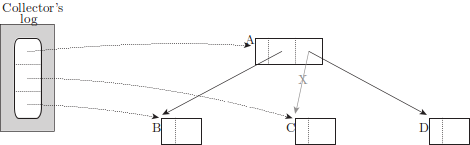
\includegraphics{figures/refcnt_1}
  \caption{Καταμέτρηση αναφορών με συγκέντρωση.}
  \label{fig:refcnt_1}  
\end{figure}

Η απλούστερη προσέγγιση στο πρόβλημα είναι ο συνδυασμός της
καταμέτρησης αναφορών με συνήθη, εφεδρική συλλογή εξιχνίασης.
Η ελπίδα είναι πώς τα περισσότερα αντικείμενα δε θα είναι 
προσβάσιμα από κύκλους και επομένως θα απελευθερώνονται
αμέσως από την καταμέτρηση αναφορών. Οι εναπομείνουσες
κυκλικές δομές συλλέγονται από το συλλέκτη εξιχνίασης. Η
ιδέα αυτή απλά μειώνει τη συχνότητα εκτέλεσης της συλλογής
εξιχνίασης. Σε επίπεδο γλώσσας, οι Friedman και Wise
\cite{DBLP:journals/ipl/FriedmanW79} παρατήρησαν πώς κύκλοι
μπορούν να δημιουργηθούν μόνο σε αγνές συναρτησιακές γλώσσες
από αναδρομικούς ορισμούς και επομένως μπορούν να
αντιμετωπιστούν ειδικά δεδομένης της παρατήρησης ορισμένων
περιορισμών.

Πολλοί ερευνητές έχουν προτείνει την ειδική αντιμετώπιση
των λειτουργιών εγγραφής δεικτών που κλείνουν κύκλους.
Μεταξύ αυτών είναι οι Friedman και Wise,
\cite{DBLP:journals/ipl/FriedmanW79}, ο BrownBridge
\cite{DBLP:conf/fpca/Brownbridge85}, ο Salkild
\cite{salkild1987implementation}; o Pepels κ.ά
\cite{pepels1988cyclic} καθώς και ο Axford
\cite{DBLP:journals/cj/Axford90}.

Οι πιο ευρέως υιοθετημένοι μηχανισμοί για το χειρισμό
κυκλικών δομών με καταμέτρηση αναφορών ωστόσο χρησιμοποιούν
μία τεχνική γνωστή και ως \textbf{δοκιμαστική διαγραφή}.
Η βασική ιδέα αφορά στο ότι δεν είναι απαραίτητο ο εφεδρικός
συλλέκτης εξιχνίασης να επισκεφτεί ολόκληρο τον γράφο των
ζωντανών αντικειμένων. Αντίθετα, αυτός μπορεί να εστιάσει
την προσοχή του σε εκείνα τα τμήματα του γράφου στα οποία
η διαγραφή ενός δείκτη μπορεί να δημιούργησε έναν κύκλο
σκουπιδιών. Ας παρατηρήσουμε πώς:

\begin{itemize}
  \item Σε κάθε κύκλο σκουπιδιών, οι μη μηδενικοί μετρητές
    αναφοράς οφείλονται σε εσωτερικούς δείκτες.
  \item Οι κύκλοι σκουπιδιών μπορεί να προκύψουν μόνο από τη
    διαγραφή κάποιου δείκτη που αφήνει το μετρητή αναφοράς
    κάποιου αντικειμένου θετικό.
\end{itemize} 

Οι αλγόριθμοι μερικής εξιχνίασης εκμεταλλεύονται τις παραπάνω
παρατηρήσεις επισκεπτόμενοι μόνο το υπογράφημα αντικειμένων
που έχει ως ρίζα κάποιο αντικείμενο το οποίο υποπτεύονται
πώς είναι σκουπίδι. Οι αλγόριθμοι αυτοί διαγράφουν δοκιμαστικά
κάθε δείκτη που συναντούν μέσω της μείωσης προσωρινά του
μετρητή αναφορών του αντικειμένου στο οποίο αυτός αναφέρεται.
Με τον τρόπο αυτό, πρακτικά αφαιρούν τη συμβολή των εσωτερικών
δεικτών στην κυκλικότητα της δομής. Αν ο μετρητής αναφορών ενός
αντικειμένου εξακολουθεί να είναι μη μηδενικός μετά από τη
διαδικασία αυτή, τότε αυτό θα πρέπει να είναι προσβάσιμο από
κάποιο αντικείμενο εκτός του υπογράφου και συνεπώς το αντικείμενο
δεν είναι σκουπίδι. Επιπλέον ούτε το μεταβατικό κλείσιμο του
αντικειμένου ως προς την προσβασιμότητα μέσω δεικτών περιέχει
σκουπίδια.

Ο Bacon κ.ά \cite{DBLP:conf/pldi/BaconALRS01}, οι Bacon
και Rajan \cite{DBLP:conf/ecoop/BaconR01} και ο Paz κ.ά
\cite{DBLP:journals/toplas/PazBKPR07} επινόησαν τον αλγόριθμο
Recycler που υποστηρίζει ταυτόχρονη κυκλική καταμέτρηση
αναφορών. Στην παρούσα φάση παρουσιάζουμε τη σύγχρονη εκδοχή
του αλγορίθμου, αναβάλλοντας την παρουσίαση της ασύγχρονης
για το κεφάλαιο 8. Ο αλγόριθμος~\ref{alg:refcnt_5} δρα σε
3 περάσματα:

\begin{algorithm}
  \caption{Κυκλική καταμέτρηση αναφορών: ο αλγόριθμος Recycler}
  \label{alg:refcnt_5}
  \begin{algorithmic}[1]
    \Function{New}{\null}
      \State $ref \gets$ \Call{allocate}{\null}
      \If{$ref = \textbf{null}$}
        \State \Call{collect}{\null} \Comment{the cycle collector}
        \State $ref \gets$ \Call{allocate}{\null}
        \If{$ref = \textbf{null}$}
          \State error ``Out of memory!''
        \EndIf
      \EndIf
      \State \Call{rc}{$ref$} $\gets 0$
      \State \Return{$ref$}
    \EndFunction
    \Statex
    \Procedure{addReference}{$ref$}
      \If{$ref \neq \textbf{null}$}
        \State \Call{rc}{$ref$} $\gets$ \Call{rc}{$ref$} $+1$
        \State \Call{colour}{$ref$} $\gets black$ \Comment{cannot be in a garbage cycle}
      \EndIf
    \EndProcedure
    \Statex
    \Procedure{deleteReference}{$ref$}
      \If{$ref \neq \textbf{null}$}
        \State \Call{rc}{$ref$} $\gets$ \Call{rc}{$ref$} $-1$
        \If{\Call{rc}{$ref$} $=0$}
          \State \Call{release}{$ref$}
        \Else
          \State \Call{candidate}{$ref$} \Comment{might isolate a garbage cycle}
        \EndIf
      \EndIf
    \EndProcedure
    \Statex
    \Procedure{release}{$ref$}
      \ForAll{$fld \; \textbf{in} \; Pointers(ref)$}
        \State \Call{deleteReference}{$fld$}
      \EndFor
      \State \Call{colour}{$ref$} $\gets black$ \Comment{objects on the free-list are black}
      \If{\textbf{not} $ref$ \textbf{in} $candidates$} \Comment{deal with candidates later}
        \State \Call{free}{$ref$}
      \EndIf
    \EndProcedure
    \Statex
    \Procedure{candidate}{$ref$} \Comment{colour as a candidate and add to the set}
      \If{\Call{colour}{$ref$} $\neq purple$}
        \State \Call{colour}{$ref$} $\gets purple$
        \State $candidates \gets candidates \cup {ref}$
      \EndIf
    \EndProcedure
    \Statex
    \Procedure{collect}{\null}
      \State \textbf{atomic}
      \ForAll{$ref \; \textbf{in} \; candidates$}
        \State \Call{scan}{$ref$}
      \EndFor
      \State \Call{collectCandidates}{\null}
    \EndProcedure
    \algstore{recycler}
  \end{algorithmic}
\end{algorithm}

\begin{algorithm}
  \ContinuedFloat
  \caption{Κυκλική καταμέτρηση αναφορών: ο αλγόριθμος Recycler (συνέχεια)}
  \begin{algorithmic}
    \algrestore{recycler}
    \Procedure{markCandidates}{\null}
      \ForAll{$ref \; \textbf{in} \; candidates$}
        \If{\Call{colour}{$ref$} $= purple$}
          \State \Call{markGrey}{$ref$} $\gets purple$
        \Else
          \State \Call{remove}{$candidates$, $ref$}
          \If{\Call{colour}{$ref$} $= purple$ \textbf{and} \Call{rc}{$ref$} $=0$}
            \State \Call{free}{$ref$}
          \EndIf
        \EndIf
      \EndFor
    \EndProcedure
    \Statex
    \Procedure{markGrey}{$ref$}
      \If{\Call{colour}{$ref$} $\neq grey$}
        \State \Call{colour}{$ref$} $\gets grey$
        \ForAll{$fld \; \textbf{in} \; Pointers(ref)$}
          \State $child \gets *fld$
          \If{$child \neq \textbf{null}$}
            \State \Call{rc}{$ref$} $\gets$ \Call{rc}{$ref$} $-1$ \Comment{trial deletion}
            \State \Call{markGrey}{$child$}
          \EndIf
        \EndFor
      \EndIf
    \EndProcedure
    \Statex
    \Procedure{scan}{$ref$}
      \If{\Call{colour}{$ref$} $= grey$}
        \If{\Call{rc}{$ref$} $>0$}
          \State \Call{scanBlack}{$ref$} \Comment{there must be an external reference}
        \Else
          \State \Call{colour}{$ref$} $\gets white$ \Comment{looks like garbage...}
          \ForAll{$fld \; \textbf{in} \; Pointers(ref)$} \Comment{...so continue}
            \State $child \gets *fld$
            \If{$child \neq \textbf{null}$}
              \State \Call{scan}{$child$}
            \EndIf
          \EndFor
        \EndIf
      \EndIf
    \EndProcedure
    \Statex
    \Procedure{scanBlack}{$ref$} \Comment{repair the reference counts of live data}
      \State \Call{colour}{$ref$} $\gets white$
      \ForAll{$fld \; \textbf{in} \; Pointers(ref)$}
        \State $child \gets *fld$
        \If{$child \neq \textbf{null}$}
          \State \Call{rc}{$ref$} $\gets$ \Call{rc}{$ref$} $+1$ \Comment{undo the trial deletion}
          \If{\Call{colour}{$child$} $\neq black$}
            \State \Call{scanBlack}{$child$}
          \EndIf
        \EndIf
      \EndFor
    \EndProcedure
    \algstore{recycler}
  \end{algorithmic}
\end{algorithm}

\begin{algorithm}
  \ContinuedFloat
  \caption{Κυκλική καταμέτρηση αναφορών: ο αλγόριθμος Recycler (συνέχεια)}
  \begin{algorithmic}
    \algrestore{recycler}
    \Procedure{collectCandidates}{\null}
      \While{\textbf{not} \Call{isEmpty}{candidates}}
        \State $ref \gets$ \Call{remove}{$candidates$}
        \State \Call{collectWhite}{$ref$}
      \EndWhile
    \EndProcedure
    \Statex
    \Procedure{collectWhite}{$ref$}
      \If{\Call{colour}{$ref$} $= white$ \textbf{and} \textbf{not} $ref$ \textbf{in} $candidates$}
        \State \Call{colour}{$ref$} $\gets black$ \Comment{free-list objects are black}
        \ForAll{$fld \; \textbf{in} \; Pointers(ref)$}
          \State $child \gets *fld$
          \If{$child \neq \textbf{null}$}
            \State \Call{collectWhite}{$child$}
          \EndIf
        \EndFor
        \State \Call{free}{$ref$}
     \EndIf
   \EndProcedure
  \end{algorithmic}
\end{algorithm}

\begin{enumerate}
  \item Αρχικά, εξιχνιάζει υπογράφους ξεκινώντας από αντικείμενα
    που αναγνωρίζονται ως πιθανά μέλη κύκλων σκουπιδιών,
    μειώνοντας τους μετρητές αναφορών που οφείλονται σε
    εσωτερικούς δείκτες (διαδικασία \textproc{markCandidates}).
    Τα επισκεπτόμενα αντικείμενα χρωματίζονται γκρι.
  \item Στη συνέχεια ελέγχει το μετρητή αναφορών κάθε τέτοιου
    αντικειμένου: αν αυτός είναι θετικός, το αντικείμενο είναι
    προσβάσιμο από κάποιο αντικείμενο που δεν ανήκει στον υπό
    εξιχνίαση υπογράφο και επομένως η δράση του πρώτου περάσματος
    αναιρείται (scan) χρωματίζοντας τα ζωντανά γκρι αντικείμενα
    μαύρα. Τα μη ζωντανά γκρι αντικείμενα χρωματίζονται λευκά.
  \item Τελικώς, όλα τα αντικείμενα ενός υπογράφου που είναι
    ακόμη λευκά είναι σκουπίδια και ελευθερώνονται.
\end{enumerate}

Με μαύρο χρώμα σημειώνονται τα ενεργά αντικείμενα ενώ με
λευκό τα σκουπίδια. Με γκρι χρώμα σημειώνονται τα αντικείμενα
που είναι πιθανά μέλη ενός κύκλου σκουπιδιών, ενώ με μωβ τα
αντικείμενα που είναι πιθανώς ρίζες ενός κύκλου σκουπιδιών.

Η διαγραφή μιας οποιασδήποτε πλην της τελευταίας αναφοράς σε
ένα αντικείμενο ενδέχεται να απομονώσει έναν κύκλο σκουπιδιών.
Σε αυτήν την περίπτωση, ο αλγόριθμος \ref{alg:refcnt_5}
χρωματίζει μωβ το αντικείμενο και το προσθέτει στη λίστα των
υποφήφιων μελών κύκλων σκουπιδιών. Διαφορετικά το αντικείμενο
είναι σκουπίδι και ο μετρητής αναφορών του οφείλει να είναι
μηδενικός. Η διαδικασία \textproc{release} επαναφέρει το χρώμα
του σε μαύρο, επεξεργάζεται αναδρομικά τα παιδιά του και αν
δεν είναι υποψήφια ρίζα κάποιου κύκλου σκουπιδιών, το
ελευθερώνει. Η ανάκτηση αντικειμένων από το σύνολο υποψηφίων
ριζών κύκλων σκουπιδιών αναβάλλεται μέχρις ότου εκτελεστεί
η διαδικασία \textproc{markCandidates}. 

Η διαδικασία \textproc{markCandidates} εξετάζει κάθε
αντικείμενο στο σύνολο υποψηφίων ριζών κύκλων σκουπιδιών.
Αν ένα αντικείμενο είναι ακόμη μωβ (δηλαδή δεν έχει προστεθεί
κάποια αναφορά σε αυτό από τη στιγμή που εισήχθη στο σύνολο),
το μεταβατικό κλείσιμο αυτού ως προς την προσβασιμότητα μέσω
δεικτών χρωματίζεται γκρι. Διαφορετικά αφαιρείται από το
σύνολο και στην περίπτωση που είναι μαύρο και ο μετρητής
αναφορών του μηδενικός, ελευθερώνεται. Η διαδικασία
\textproc{markGrey} χρωματίζει γκρι τον υπογράφο που έχει ως
ρίζα το εν λόγω αντικείμενο και αφαιρεί από τους μετρητές
αναφορών των αντικειμένων του υπογράφου τη συμβολή των
εσωτερικών δεικτών.

\begin{figure}[H]
  \centering
  \begin{subfigure}{1.0\textwidth}
    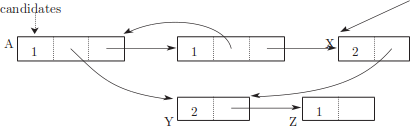
\includegraphics{figures/refcnt_2a}
    \caption{Πριν τη διαδικασία \textproc{markGrey}.}
  \end{subfigure}

  \begin{subfigure}[b]{1.0\textwidth}
    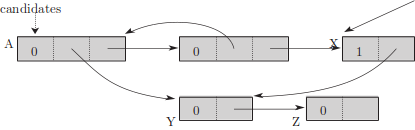
\includegraphics{figures/refcnt_2b}
    \caption
      {Μετά τη \textproc{markGrey}, όλα τα αντικείμενα που
       είναι προσβάσιμα από ένα αντικείμενο υποψήφιο μέλος
       κύκλου σκουπιδιών έχουν σημανθεί γκρι και η επίδραση
       των εσωτερικών δεικτών αυτού του γκρι υπογράφου έχει
       αφαιρεθεί. Ο μετρητής αναφορών του αντικειμένου $X$,
       το οποίο είναι ακόμη προσβάσιμο, έχει μη μηδενική
       τιμή.}
  \end{subfigure}
  
  \begin{subfigure}[b]{1.0\textwidth}
    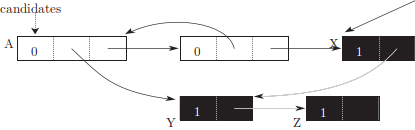
\includegraphics{figures/refcnt_2c}
    \caption
      {Μετά τη \textproc{scan}, όλα τα προσβάσιμα αντικείμενα
       είναι μαύρα και οι μετρητές αναφορών αυτών έχουν
       επιδιορθωθεί και αντικατοπτρίζουν ζωντανές αναφορές.}
  \end{subfigure}
  \caption[Κυκλική καταμέτρηση αναφορών.]
    {Κυκλική καταμέτρηση αναφορών. Το πρώτο πεδίο κάθε
     αντικειμένου αποθηκεύει το μετρητή αναφορών του.}
  \label{fig:refcnt_2}
\end{figure}

Στη δεύτερη φάση της συλλογής, εξετάζονται οι μετρητές
αναφορών κάθε αντικειμένου που είναι υποψήφια ρίζα ενός
κύκλου σκουπιδιών καθώς και των αντικειμένων που ανήκουν
στο μεταβατικό κλείσιμο αυτού ως προς την προσβασιμότητα
μέσω δεικτών. Αν ο μετρητής αναφορών ενός αντικειμένου
βρεθεί θετικός, τότε σίγουρα υπάρχει εξωτερική αναφορά
προς αυτό. Στην περίπτωση αυτή, η διαδικασία
\textproc{scanBlack} αναιρεί την επίδραση της διαδικασίας
\textproc{markGrey} αυξάνοντας το μετρητή αναφοράς και
χρωματίζοντας το αντικείμενο μαύρο. Αντίθετα, αν ο μετρητής
αναφορών είναι μηδενικός, η διαδικασία \textproc{scan}
χρωματίζει το αντικείμενο λευκό και εξετάζει αναδρομικά τα
παιδιά του. Στο σημείο αυτό δε μπορούμε με βεβαιότητα να
υποθέσουμε πώς ένα λευκό αντικείμενο είναι σκουπίδι, καθώς
αυτό μπορεί να επανεξετασθεί αργότερα από κλήση της
διαδικασίας \textproc{scanBlack} με όρισμα κάποιο άλλο
αντικείμενο του υπογράφου.

Τέλος, η τρίτη φάση, η οποία υλοποιείται από τη διαδικασία
\textproc{collectWhite} αποδεσμεύει τα λευκά αντικείμενα.
Επαναληπτικά, μέχρις ότου αδειάσει το σύνολο υποψηφίων ριζών
κύκλων σκουπιδιών αφαιρείται από αυτό ένα αντικείμενο και
εξετάζεται το χρώμα του. Αν είναι λευκό, το αντικείμενο
ελευθερώενεται (χρωματίζεται μαύρο) και στη συνέχεια
εξετάζονται αναδρομικά τα παιδιά του. Η διαδικασία
\textproc{collectWhite} δεν επεξεργάζεται αντικείμενα
παιδιά που τυχαίνει να βρίσκονται στο σύνολο των υποψηφίων
ριζών κύκλων σκουπιδιών: η ελευθέρωσή τους πραγματοποιείται
σε επόμενη επανάληψη του βρόχου της διαδικασίας
\textproc{collectCandidates}.

Ο αλγόριθμος Recycler μπορεί να βελτιστοποιηθεί περαιτέρω με
την στατική αναγνώριση πώς αντικείμενα συγκεκριμένων κλάσεων
δε μπορούν να είναι μέλη κύκλων σκουπιδιών (όπως για παράδειγμα
αντικείμενα που δεν περιέχουν δείκτες, αλλά όχι μόνο) και
ως εκ τούτου δε χρειάζεται να μπουν στο σύνολο των υποψήφιων
ριζών κύκλων σκουπιδιών. Τα αντικείμενα αυτά χρωματίζονται
πράσινα και όχι μαύρα. Οι Bacon και Rajan
\cite{DBLP:conf/ecoop/BaconR01} διαπιστώνουν πώς αυτή η
βελτιστοποίηση μειώνει κατά μία τάξη μεγέθους το μέγεθος
του συνόλου υποψηφίων ριζών κύκλων σκουπιδιών. 

\section{Ανακεφαλαίωση και θέματα προς εξέταση}
Η καταμέτρηση αναφορών είναι ελκυστική για την προθυμία
συλλογής αντικειμένων σκουπιδιών αλλά και τις ιδιότητες
τοπικότητας αυτής. Η απλοϊκή καταμέτρηση αναφορών μπορεί
να ανακτήσει τη μνήμη από ένα αντικείμενο αμέσως μόλις
αφαιρείται ο τελευταίος δείκτης που αναφέρεται σε αυτό.
Η λειτουργία της εμπλέκει μόνο τους παλαιούς και νέους
στόχους των δεικτών που εγγράφονται ή διαβάζονται, σε
αντίθεση με τη συλλογή εξιχνίασης που επισκέπτεται κάθε
ζωντανό αντικείμενο στο σωρό. Ωστόσο, τα πλεονεκτήματα
της μεθόδου είναι ταυτόχρονα και τα μειονεκτήματα της.
Καθώς δεν μπορεί να ελευθερώσει ένα αντικείμενο μέχρις
ότου κανένας δείκτης δεν αναφέρεται σε αυτό, δεν μπορεί
να συλλέξει κύκλους σκουπιδιών. Επιπλέον, προσθέτει ένα
μικρό κόστος σε κάθε λειτουργία \textproc{Read} και
\textproc{Write} του τροποποιητή, επιβαρύνοντας με τον
τρόπο αυτό τη ρυθμαπόδοση του τελευταίου περισσότερο σε
σχέση με τη συλλογή εξιχνίασης. Επιπλέον, οι πολυνηματικές
εφαρμογές απαιτούν τον αυστηρό συγχρονισμό των τροποποιήσεων
των μετρητών αναφορών και των ενημερώσεων δεικτών. Τέλος,
η συλλογή σκουπιδιών με καταμέτρηση αναφορών αυξάνει το
μέγεθος των αντικειμένων.

\subsection{Περιβάλλον εκτέλεσης}
Παρά τα παραπάνω ζητήματα, ο αποκλεισμός της καταμέτρησης
αναφορών χωρίς περαιτέρω σκέψη είναι εσφαλμένος. Ασφαλώς
και δεν είναι κατάλληλη ως τμήμα του διαχειριστή μνήμης
μιας εικονικής μηχανής γενικού σκοπού, ειδικά αν τα
εμπλεκόμενα αντικείμενα είναι μικρά, εμφανίζονται συχνά
κύκλοι και ο ρυθμός λειτουργιών εγγραφής δεικτών από τον
τροποποιητή είναι υψηλός. Ωστόσο, υπάρχουν περιβάλλοντα
στα οποία η χρήση καταμέτρησης αναφορών είναι κατάλληλη.
Η καταμέτρηση αναφορών αποδεικνύεται αποδοτική σε
περιβάλλοντα όπου οι χρόνοι ζωής των περισσότερων
αντικειμένων είναι αρκετά απλοί ώστε αυτά να διαχειρίζονται
ρητώς. Μπορεί επίσης να περιορισθεί στη διαχείριση ενός
μικρότερου αριθμού πόρων με πιο σύνθετες σχέσεις
ιδιοκτησίας. Συχνά οι πόροι αυτοί είναι μεγάλα αντικείμενα
με αποτέλεσμα το κόστος της προσθήκης στην επικεφαλίδα μιας
λέξης για την αποθήκευση του μετρητή αναφοράς να είναι
αμελητέο. Δεδομένα όπως bitmaps ψηφιακών εικόνων δεν
περιλαμβάνουν δείκτες και συνεπώς είναι αδύνατη η εμφάνιση
κύκλων σκουπιδιών. Επιπρόσθετα, η καταμέτρηση αναφορών
μπορεί να υλοποιηθεί ως τμήμα μιας βιβλιοθήκης και όχι
ως τμήμα του συστήματος εκτέλεσης, δίνοντας με τον τρόπο
αυτό πλήρη έλεγχο στον προγραμματιστή όσον αφορά τη χρήση
της. Στην περίπτωση αυτή βέβαια απαιτείται ιδιαίτερη
προσοχή από τον προγραμματιστή, ο οποίος πρέπει να
εξασφαλίσει την απουσία καταστάσεων συναγωνισμού μεταξύ
λειτουργιών εγγραφής δεικτών και ενημερώσεων μετρητών
αναφορών.

\subsection{Προηγμένες τεχνικές}
Εξεζητημένοι αλγόριθμοι καταμέτρησης αναφορών προσφέρουν
λύσεις για τα περισσότερα από τα προβλήματα που αντιμετωπίζει
η απλοϊκή καταμέτρηση αναφορών, επιβάλλοντας ωστόσο παύση
του κόσμου, όπως συμβαίνει και στη συλλογή εξιχνίασης.

Η μνήμη αντικειμένων ενός κύκλου σκουπιδιών μπορεί να ανακτηθεί
από ένα εφεδρικό συλλέκτη εξιχνίασης, ή χρησιμοποιώντας την
τεχνική της δοκιμαστικής διαγραφής. Και στις δύο περιπτώσεις,
η εκτέλεση του τροποποιητή αναστέλλεται κατά τη διάρκεια
συλλογής των κύκλων σκουπιδιών.

Παρότι στη χειρότερη περίπτωση το πεδίο ενός αντικειμένου
όπου αποθηκεύεται ο μετρητής αναφορών πρέπει να είναι τόσο
μεγάλο ώστε να χωράει το μέγιστο πλήθος δεικτών, οι
περισσότερες εφαρμογές διατηρούν μικρό αριθμό αναφορών προς
τα περισσότερα αντικείμενα. Συχνά, είναι δυνατό να κλαπούν
μερικά bits από μια λέξη της επικεφαλίδας που χρησιμοποιείται
για την αποθήκευση ενός κλειδώματος ή ενός κωδικού
κατακερματισμού. Είναι βέβαια επίσης σύνηθες να υπάρχουν
πολλές αναφορές προς μερικά αντικείμενα.

Η επιβάρυνση στη ρυθμαπόδοση του τροποποιητή μπορεί να
μειωθεί παραλείποντας μερικές τροποποιήσεις δεικτών και
μειώνοντας το κόστος άλλων. Η καταμέτρηση αναφορών με
αναβολή αγνοεί τις εγγραφές από τον τροποποιητή των τοπικών
μεταβλητών. Αυτό επιτρέπει στους μετρητές αναφορών των
αντικειμένων που είναι προσβάσιμα από τις ρίζες να έχουν
μικρότερη τιμή από πραγματική και αποτρέπει την πρόωρη
ανάκτηση της μνήμης που αυτά καταλαμβάνουν. Η καταμέτρηση
αναφορών με συγκέντρωση λαμβάνει υπόψη την κατάσταση ενός
αντικειμένου μόνο στην αρχή και στο τέλος μιας εποχής,
αγνοώντας τις λειτουργίες εγγραφής δεικτών στο ενδιάμεσο
χρονικό διάστημα. Κατά κάποιο τρόπο είναι μια αυτόματη
βελτιστοποίηση: αφαιρεί τις περιττές ενδιάμεσες
επιδιορθώσεις των μετρητών αναφορών. Ωστόσο και πάλι,
τόσο η καταμέτρηση αναφορών με αναβολή όσο και η καταμέτρηση
αναφορών με συγκέντρωση επιβάλλουν την παύση του κόσμου
για ένα χρονικό διάστημα ώστε να επιδιορθωθούν οι μετρητές
αναφορών. Επιπλέον, προσθέτουν μία επιβάρυνση στις
απαιτήσεις σε χώρο της απλοϊκής καταμέτρησης αναφορών
για την αποθήκευση είτε του πίνακα μηδενικών μετρητών
αναφορών είτε των απομονωτών καταγραφής ενημερώσεων.

Ένα επιπρόσθετο πλεονέκτημα των προηγμένων αυτών τεχνικών
συλλογής με καταμέτρηση αναφορών είναι πώς κλιμακώνουν
καλά με μεγάλους σωρούς. Το κόστος τους είναι ανάλογο
μόνο προς τον αριθμό των εγγραφών δεικτών και όχι του
όγκου των δεδομένων ζωντανών αντικειμένων.
\end{greek}

\part{Προηγμένοι αλγόριθμοι συλλογής σκουπιδιών}
\begin{greek}
\chapter{Γενεαλογική συλλογή σκουπιδιών}\label{ch:gen}

Ο στόχος ενός συλλέκτη σκουπιδιών είναι η εύρεση νεκρών αντικειμένων
και εν συνεχεία η αποδέσμευση του χώρου που αυτά καταλαμβάνουν.
Οι συλλέκτες εξιχνίασης (και ειδικότερα οι συλλέκτες με αντιγραφή)
παρουσιάζουν καλές επιδόσεις όταν ο σωρός περιλαμβάνει σχετικά
λίγα ζωντανά αντικείμενα. Δε μεταχειρίζονται ωστόσο αποδοτικά
αντικείμενα με μακρά διάρκεια ζωής, τα οποία είτε σημαίνουν και
ξε-σημαίνουν είτε αντιγράφουν από τον ένα ημιχώρο στον άλλο
διαρκώς. Είδαμε στο κεφάλαιο~\ref{ch:mrkcmp} πώς αντικείμενα με
μακρά διάρκεια ζωής τείνουν να συγκεντρώνονται στο κάτω μέρος
του σωρού όταν αυτός διαχειρίζεται από ένα συλλέκτη με σήμανση
και συμπύκνωση και πώς πολλοί συλλέκτες αποφεύγουν τη συμπύκνωση
αυτού του τμήματος. Παρότι αυτή η βελτιστοποίηση αφαιρεί το κόστος
της μετακίνησης αυτών, τα εν λόγω αντικείμενα πρέπει να εξετάζονται
και τα πεδία δείκτες αυτών να ενημερώνονται σε κάθε κύκλο συλλογής. 

Οι γενεαλογικοί συλλέκτες σκουπιδιών επεκτείνουν την παραπάνω
ιδέα αγνοώντας τα παλαιότερα αντικείμενα οποτεδήποτε αυτό είναι
δυνατό. Οι συλλέκτες αυτής της κατηγορίας βασίζονται στην ασθενή
γενεαλογική υπόθεση πώς τα περισσότερα αντικείμενα πεθαίνουν νέα.
Επικεντρώνοντας την προσοχή τους στα νεότερα αντικείμενα, προσπαθούν
να μεγιστοποιήσουν τον ελεύθερο χώρο που ανακτούν με το λιγότερο
δυνατό κόπο. Κατηγοριοποιούν τα αντικείμενα με βάση την ηλικία
τους σε γενεές, με την κάθε γενιά να ζει συνήθως σε ένα ξεχωριστό
τμήμα του σωρού. Οι γενεές συλλέγονται σε αύξουσα σειρά ως προς
την ηλικία  τους, ενώ  τα αντικείμενα που επιβιώνουν μετά από
αρκετούς κύκλους συλλογής προάγονται σε παλαιότερες γενεές.

Οι περισσότεροι συλλέκτες αυτής της κατηγορίας διαχειρίζονται
τις νεότερες γενεές με αντιγραφή. Ο απαιτούμενος χρόνος που
δαπανάται για τη νεότερη γενεά, γνωστή και ως βρεφοκομείο εξαρτάται
από το μέγεθός της. Ρυθμίζοντας επομένως το μέγεθος αυτό, μπορούμε
να ελέγξουμε το χρόνο παύσης για τη συλλογή μιας γενεάς. Οι χρόνοι
παύσης για τη συλλογή των νεότερων γενεών σε εφαρμογές που τρέχουν
σε ένα σύγχρονο μηχάνημα και οι οποίες επαληθεύουν την ασθενή
γενεαλογική υπόθεση είναι της τάξης των χιλιοστών του δευτερολέπτου.
Θεωρώντας ακόμη πώς η συλλογή εκτελείται σχετικά αραιά, η δράση
ενός γενεαλογικού συλλέκτη περνάει σχεδόν απαρατήρητη στον τροποποιητή.

Αν ένας γενεαλογικός συλλέκτης εκτιμήσει πώς η συλλογή μόνο
της νεότερης γενιάς δε θα ανακυκλώσει αρκετό χώρο, χρειάζεται
να συλλεχθεί ολόκληρος ο σωρός. Συνεπώς η γενεαλογική συλλογή
σκουπιδιών βελτιώνει μόνο την αναμενόμενη τιμή του χρόνου παύσης
και όχι την χείριστη περίπτωση. Δεν επαρκεί από μόνη της για ένα
σύστημα πραγματικού χρόνου.

Η \textbf{γενεαλογική συλλογή σκουπιδιών} δεν είναι τελείως
δωρεάν. Αρχικά η συνεχόμενη συλλογή μόνο των νεότερων γενεών
δεν μπορεί να εντοπίσει σκουπίδια που ζουν σε παλαιότερες γενεές.
Επιπλέον, για να μπορεί να συλλέξει μόνο μια γενεά, αγνοώντας
τις υπόλοιπες, ο συλλέκτης θα πρέπει με κάποιο τρόπο να σημειώνει
τους δείκτες που διασχίζουν τα σύνορα μεταξύ των γενεών.

\section{Πώς μετράται ο χρόνος;}
Για να πρoάγει ένας γενεαλογικός συλλέκτης αντικείμενα από μία γενεά σε μία 
παλαιότερη, απαιτείται να μπορεί να προσδιορίζει πόσο παλαιά αυτά είναι. 
Επομένως χρειάζεται τόσο ένα μηχανισμό μέτρησης του χρόνου όσο και ένα μηχανισμό 
μέτρησης της ηλικίας των αντικειμένων. Στη βιβλιογραφία συναντώνται κυρίως δύο 
πιθανές μετρικές: το συνολικό μέγεθος της δεσμευμένης μνήμης και ο χρόνος που 
έχει περάσει από την έναρξη της εκτέλεσης της εφαρμογής. Η μετρική του χρόνου 
καθορίζει το προφίλ της εφαρμογής. Απαντάει σε ερωτήσεις που αφορούν το για πόσο 
τρέχει μια εφαρμογή καθώς και ποιοι είναι οι χρόνοι παύσης αυτής και είναι 
κατανεμημένοι. Απαντήσεις στις ερωτήσεις αυτές μπορούν να χρησιμοποιηθούν ώστε 
να αποφανθεί κανείς σχετικά με την αποκρισιμότητα της εφαρμογής και το κατά πόσο 
η διακοπή αυτής για συλλογή σκουπιδιών ενοχλεί έναν διαδραστικό χρήστη. Από την 
άλλη πλευρά, εσωτερικά, η διαφορά σε bytes της συνολικής δεσμευμένης μνήμης στο 
σωρό μεταξύ των χρονικών στιγμών της γέννησης και του θανάτου ενός αντικειμένου 
αντικατοπτρίζει καλύτερα τη χρονική διάρκεια ζωής αυτού. Είναι επίσης ένα μέγεθος 
ανεξάρτητο της αρχιτεκτονικής. Τέλος, αποτελεί στοιχείο των απαιτήσεων σε μνήμη 
μιας εφαρμογής και είναι στενά συνδεδεμένο με τη συχνότητα με την οποία θα κληθεί 
ο συλλέκτης. Η μέτρηση του χρόνου με όρους bytes είναι ιδιαίτερα επίπονη διαδικασία 
σε πολυεπεξεργαστικά περιβάλλοντα όπου εκτελούνται ταυτόχρονα πολλά νήματα. Η χρήση 
ενός απλού καθολικού μετρητή του συνολικού μεγέθους της δεσμευμένης μνήμης ενδέχεται 
να παραπλανήσει το συλλέκτη σχετικά με την ηλικία ενός αντικειμένου, καθώς μια 
μεγάλη τιμή του μπορεί να έχει προκύψει από την εκχώρηση μνήμης σε νήματα άσχετα 
με το αντικείμενο. Οι πραγματικές υλοποιήσεις γενεαλογικών συλλεκτών σκουπιδιών 
μοντελοποιούν την ηλικία ενός αντικειμένου ως τον αριθμό των συλλογών από τις 
οποίες αυτό έχει επιβιώσει.

\section{Γενεαλογικές υποθέσεις}
\textbf{H ασθενής γενεαλογική υπόθεση}, σύμφωνα με την οποία
τα περισσότερα αντικείμενα πεθαίνουν νέα, φαίνεται γενικώς
έγκυρη, ανεξαρτήτως της γλώσσας προγραμματισμού. Οι Foderaro
και Fateman \cite{DBLP:conf/issac/FoderaroF81} διαπίστωσαν
πώς σε ένα πακέτο υπολογιστικής άλγεβρας γραμμένο στη γλώσσα
MacLisp, το 98\% της μνήμης που ανακτούσε ένας κύκλος συλλογής
είχε εκχωρηθεί μετά το πέρας του προηγούμενου κύκλου. Ο Zorn
\cite{Zorn:CSD-89-544} ανέφερε πώς το ποσοστό των αντικειμένων
στη γλώσσα Common Lisp τα οποία επιβίωναν λιγότερο από 10 ΚΒ
εκχώρησης κυμαίνεται μεταξύ 50\% και 90\%. Αντίστοιχα συμπεράσματα 
ισχύουν και για τις συναρτησιακές γλώσσες προγραμματισμού. Οι
Sansom και Simon Peyton Jones \cite{DBLP:conf/fpca/SansomJ93},
παρατήρησαν, πώς στη Haskell, ένα ποσοστό μεταξύ 75\% και 95\%
των αντικειμένων του σωρού πεθαίνουν πριν την ηλικία των 10 KB
και πώς μόνο το 5\% των αντικειμένων ζουν περισσότερο από 1 ΜΒ.
Ο Appel παρατήρησε πώς στην Standard ML/NJ, σε κάθε κύκλο
συλλογής, το 98\% της μνήμης κάθε γενεάς ελευθερώνεται, ενώ
οι Stefanovic και Moss \cite{DBLP:conf/lfp/StefanovicM94}
βρήκαν πώς μόνο ένα ποσοστό από 2\% έως 8\% αντικειμένων του
σωρού επιβίωναν μετά το κατώφλι των 100 ΚΒ.

Η υπόθεση ισχύει και για πολλά προγράμματα γραμμένα σε
αντικειμενοστρεφείς γλώσσες. Ο Ungar \cite{Ungar:CSD-86-287}
βρήκε πώς λιγότερο από το 7\% των αντικειμένων στη Smalltalk
ζουν πέραν των 140 KB. Οι Dieckmann και H{\"o}lzle
\cite{DBLP:conf/ecoop/DieckmannH99} ανέφεραν πώς ο όγκος των
ζωντανών Java αντικειμένων στη σουίτα benchmark SPECjvm98
που επιβίωναν τα 100 KB εκχώρησης κυμαινόταν μεταξύ 1\%
και 40\% και πώς λιγότερο από το 21 \% ζούσε πέραν του 1 ΜΒ
παρότι το ποσοστό διέφερε σημαντικά από εφαρμογή σε εφαρμογή.
Ο Blackburn κ.ά \cite{DBLP:conf/oopsla/BlackburnGHKMBDFFGHHJLMPSVDW06}
βρήκαν πώς κατά μέσο όρο ένα ποσοστό μικρότερο του 9\% των
αντικειμένων που εκχωρούνταν στις εφαρμογές των σουιτών
benchmark SPECjvm98 και DaCapo γλίτωνε από τα 4 MB παρότι
υπήρχε μεγάλη απόκλιση ανάμεσα στα διαφορετικά benchmark.
Αυτό βέβαια ήταν ένα άνω φράγμα του ποσοστού των αντικειμένων
που ζούσαν πέραν των 4 MB, καθώς μερικά επιζώντα αντικείμενα
μπορεί να γλίτωναν καθώς εκχωρούνταν σχεδόν αμέσως μετά από
μια συλλογή της νεότερης γενεάς. Οι Jones και Ryder \cite{DBLP:conf/iwmm/JonesR08}
πώς η διάρκεια ζωής των αντικειμένων εφαρμογών Java ακολουθούσαν
τη διωνυμική κατανομή: ένα ποσοστό μεταξύ 65\% και 96\% των
αντικειμένων στις εφαρμογές της σουίτας benchmark DaCapo
δεν επιβίωναν μετά τα 64 KB, ενώ ένα ποσοστό μεταξύ 3\%
και 16\% ήταν αθάνατα ή ζούσαν και πέραν των 4 MB. Ακόμη
και στις προστακτικές γλώσσες προγραμματισμού όπου δεν υπάρχει
αυτόματη διαχείριση μνήμης, η διάρκεια ζωής πολλών αντικειμένων
είναι μικρή. Οι Barrett και Zorn \cite{DBLP:conf/pldi/BarrettZ93}
ανέφεραν πώς παραπάνω από το 50\% των εκχωρηθέντων στο σωρό
αντικειμένων πέθαιναν κάποια στιγμή πριν τα 10 KB και λιγότερο
από το 10\% επιβίωνε πέραν των 32 KB.

Από την άλλη πλευρά, υπάρχουν εμφανώς λιγότερες ενδείξεις
που να επιβεβαιώνουν την \textbf{ισχυρή γενεαλογική υπόθεση}
του Hayes \cite{DBLP:conf/oopsla/Hayes91}, σύμφωνα με την
οποία ακόμη και για τα αντικείμενα που δε δημιουργήθηκαν
πρόσφατα, ισχύει πώς τα νεότερα αντικείμενα θα έχουν μικρότερο
ρυθμό επιβίωσης από τα παλαιότερα. Το απλό μοντέλο της ασθενούς
γενεαλογικούς υπόθεσης περιγράφει ικανοποιητικά τη γενική
συμπεριφορά των αντικειμένων. Ωστόσο, εξαιρώντας τα αντικείμενα
που πεθαίνουν νέα, η δημογραφία των αντικειμένων σε μία
ευρύτερη χρονική κλίμακα είναι πιο πολύπλοκη. Οι χρόνοι
ζωής των αντικειμένων δεν είναι τυχαίοι. Όπως παρατηρούν
οι Dieckmann και H{\"o}lzle \cite{DBLP:conf/ecoop/DieckmannH99}
και οι Jones και Ryder \cite{DBLP:conf/iwmm/JonesR08}, επειδή
τα προγράμματα λειτουργούν σε φάσεις, τα αντικείμενα έχουν
την τάση να ζουν σε συστάδες και να πεθαίνουν όλα μαζί
ταυτόχρονα. Επιπλέον, ένας σημαντικό πλήθος αντικειμένων μπορεί
να μην πεθάνει ποτέ. Κάποιοι ερευνητές έχουν ακόμη ισχυρισθεί
πώς ενδέχεται να υπάρχει ένας συσχετισμός μεταξύ της διάρκειας
ζωής των αντικειμένων και του μεγέθους τους. Οι απόψεις πάντως
\cite{DBLP:conf/oopsla/CaudillW86, DBLP:conf/oopsla/UngarJ88,
DBLP:conf/pldi/BarrettZ93} σχετικά το κατά πόσο ο ισχυρισμός
είναι αληθής διαφέρουν.

\section{Γενεές και οργάνωση σωρού}
Μια ευρεία γκάμα στρατηγικών έχει προταθεί στη βιβλιογραφία για την οργάνωση των
γενεών. Οι γενεαλογικοί συλλέκτες μπορεί να χρησιμοποιούν δύο ή και περισσότερες
γενεές, οι οποίες μπορεί να διαχωρίζονται φυσικά ή λογικά. Το μέγεθος μιας γενεάς
μπορεί να είναι σταθερό και φραγμένο ή μπορεί να απαιτείται συμβιβασμός μεταξύ των 
μεγεθών των διαφόρων υποχώρων του σωρού. Μια γενεά μπορεί να είναι επίπεδη στο
εσωτερικό της ή να περιλαμβάνει έναν αριθμό από υποχώρους που χαρακτηρίζονται
με βάση την ηλικία και είναι γνωστοί ως \textbf{κάδοι}. Μια γενεά ενδέχεται
επίσης να περιέχει το δικό της υποχώρο για μεγάλα αντικείμενα. Τέλος, κάθε γενεά
μπορεί να μεταχειρίζεται από διαφορετικό αλγόριθμο.

Οι πρωταρχικοί στόχοι της γενεαλογικής συλλογής σκουπιδιών είναι η μείωση των
χρόνων παύσης και η βελτίωση της διεκπεραιωτικής ικανότητας. Υποθέτοντας πώς η
διαχείριση της νεότερης γενεάς έχει ανατεθεί σε ένα συλλέκτη αντιγραφής, οι αναμενόμενοι
χρόνοι παύσης εξαρτώνται κατά κύριο λόγο από τον όγκο των ζωντανών αντικειμένων
που επιβιώνουν από μία \textbf{μικρή} συλλογή της γενεάς αυτής, ο οποίος
με τη σειρά του εξαρτάται από το μέγεθος αυτής. Αν ωστόσο το μέγεθος του βρεφοκομείου
είναι πολύ μικρό και συνεπώς η συλλογή πολύ γρήγορη, το ποσό της μνήμης που θα 
ελευθερωθεί θα είναι μικρό, καθώς τα αντικείμενα του βρεφοκομείου δεν έχουν
επαρκή χρόνο για να πεθάνουν. Το γεγονός αυτό ενδέχεται να έχει πολλές ανεπιθύμητες
επιπτώσεις. 

Πρώτον, θα αυξηθεί σημαντικά η συχνότητα συλλογής της νεότερης γενεάς. Παράλληλα, το 
κόστος της αντιγραφής, το οποίο είναι ανάλογο του πλήθους των αντικειμένων που επιβιώνουν 
αναμένεται να αυξηθεί επίσης, δεδομένου ότι τα αντικείμενα θα έχουν λιγότερο χρόνο
ώστε να πεθάνουν. Επίσης, κάθε κύκλος συλλογής απαιτεί την αναστολή των νημάτων του
τροποποιητή και το σκανάρισμα της στοίβας κάθε νήματος.

Δεύτερον, η παλαιότερη γενεά αναμένεται να γεμίσει πολύ γρήγορα με συνέπεια να χρειαστεί
να συλλεγεί και αυτή συντομότερα. Υψηλοί ρυθμοί προώθησης θα προκαλέσουν αύξηση της
συχνότητας συλλογής της παλαιότερης γενεάς ή και όλων των γενεών. Επιπροσθέτως, η
πρόωρη προώθηση αντικειμένων αυξάνει την πιθανότητα της εμφάνισης ``οικογενειοκρατίας'',
καθώς αντικείμενα που έχουν εγκατασταθεί μόνιμα στην παλαιά γενιά διατηρούν εν ζωή τους
νεκρούς απογόνους τους στη νέα γενεά, προκαλώντας μία τεχνητή αύξηση του ρυθμού 
επιβίωσης.
 
Τρίτον, υπάρχουν σημαντικές ενδείξεις πώς τα προσφάτως δημιουργηθέντα αντικείμενα
τροποποιούνται συχνότερα από ότι τα παλαιότερα. Αν τα αντικείμενα αυτά προωθηθούν 
πρόωρα, ο υψηλός ρυθμός επεξεργασίας τους θα προσθέσει επιπλέον πίεση στις λειτουργίες
εγγραφής του τροποποιητή. Αυτό είναι ιδιαίτερα ανεπιθύμητο, ειδικά στην περίπτωση όπου
το κόστος του φράγματος εγγραφής είναι υψηλό. 

Τέλος, η προώθηση αντικειμένων προκαλεί την αραίωση των δεδομένων επεξεργασίας ενός
προγράμματος. Η ταυτόχρονη ελαχιστοποίηση του χρόνου διάρκειας των μικρών συλλογών καθώς 
και του πλήθους των \textbf{μεγάλων} και πιο ακριβών συλλογών από τη μία πλευρά, 
και η αποφυγή της σημαντικής επιβάρυνσης του τροποποιητή με ενέργειες που αφορούν στην 
αυτόματη διαχείριση μνήμης από την άλλη, είναι οι δύο αντικρουόμενοι στόχοι μεταξύ των 
οποίων η γενεαλογική οργάνωση προσπαθεί να επιτύχει συμβιβασμό.

\section{Πολλαπλές γενεές}
Η προσθήκη περισσότερων γενεών αποτελεί μία απάντηση στο δίλημμα του πώς να διατηρηθούν
μικροί χρόνοι παύσης για τις συλλογές του βρεφοκομείου ενώ ταυτόχρονα να αποφεύγονται οι
πλήρεις συλλογές λόγω του ότι η παλαιότερη γενεά γεμίζει γρήγορα. Ο ρόλος των ενδιάμεσων
γενεών αφορά το φιλτράρισμα εκείνων των αντικειμένων που έχουν επιβιώσει τη συλλογή της 
νεότερης γενεάς και δε ζουν πολύ ακόμα. Εάν ένας συλλέκτης προωθεί όλα τα ζωντανά
αντικείμενα \textbf{μαζικά} από τη νεότερη γενεά, στους επιζώντες θα 
περιλαμβάνονται και τα προσφάτως δημιουργηθέντα αντικείμενα παρά το ότι αυτά αναμένεται
να πεθάνουν σύντομα. Με τη χρήση πολλαπλών γενεών, το μέγεθος της μικρότερης γενεάς
δύναται να κρατηθεί αρκετά μικρό ώστε να ικανοποιούνται οι απαιτήσεις που αφορούν στους
χρόνους παύσης χωρίς να αυξάνεται ο όγκος των δεδομένων που πεθαίνουν στην παλαιότερη
γενεά σύντομα μετά την προαγωγή τους σε αυτή.

Η χρήση πολλαπλών γενεών μπορεί να έχει πολλαπλά μειονεκτήματα. Τα περισσότερα συστήματα
συλλέγουν όλες τις νέες γενεές πριν συλλέξουν την παλαιότερη. Η τεχνική προσφέρει το
πλεονέκτημα πώς απαιτείται η καταγραφή μόνο των δεικτών από αντικείμενα μιας παλιάς γενεάς
προς αντικείμενα μιας νέας. Δυστυχώς όμως οι δείκτες αυτοί εμφανίζονται σπανιότερα από
ότι οι αντίστοιχοι δείκτες με αντίστροφη κατεύθυνση. Παρότι ο απαιτούμενος χρόνος για τη
συλλογή μιας ενδιάμεσης γενεάς είναι μικρότερος από τον αντίστοιχο χρόνο για τη συλλογή
ολόκληρου του σωρού, οι χρόνοι παύσης θα είναι μεγαλύτεροι από τους αντίστοιχους χρόνους
παύσης της συλλογής της νεότερης γενιάς μόνο. Οι γενεαλογικοί συλλέκτες πολλαπλών γενεών
επίσης είναι πιο σύνθετοι στην υλοποίηση και μπορεί να εισάγουν επιπρόσθετα κόστη: το
κρίσιμο από άποψη επίδοσης τμήμα του κώδικα που υλοποιεί την εξερεύνηση του γράφου των
αντικειμένων καλείται να ξεχωρίζει ανάμεσα σε πολλές γενεές και όχι μόνο δύο (κάτι το
οποίο συνήθως πραγματοποιείται με έναν απλό έλεγχο έναντι μιας διεύθυνσης, η οποία μπορεί
να είναι μία σταθερά μεταγλώττισης). Η αύξηση των γενεών επίσης αναμένεται να αυξήσει
το πλήθος των δημιουργούμενων διαγενεαλογικών δεικτών, γεγονός το οποίο με τη σειρά του
ενδέχεται να αυξήσει την πίεση στο φράγμα εγγραφής του τροποποιητή. Τέλος, η οργάνωση του
σωρού σε πολλαπλές γενεές τείνει να αυξάνει το μέγεθος του συνόλου ριζών των νεότερων 
γενεών καθώς προάγονται αντικείμενα τα οποία δε θα είχαν προαχθεί αν ο χώρος των 
ενδιάμεσων γενεών είχε χρησιμοποιηθεί για την αύξηση του μεγέθους της νεότερης γενεάς.

Παρότι πολλοί αρχικοί γενεαλογικοί συλλέκτες για τις γλώσσες Smalltalk και Lisp
λειτουργούσαν με πολλές γενεές, σχεδόν όλοι οι σύγχρονοι γενεαλογικοί συλλέκτες για
αντικειμενοστρεφείς γλώσσες χρησιμοποιούν μόνο δύο. Ακόμη και όταν ο σωρός οργανώνεται
σε περισσότερες των δύο γενεές, όπως για παράδειγμα συμβαίνει στις υλοποιήσεις
συναρτησιακών γλωσσών όπου οι ρυθμοί γέννησης και θνησιμότητας αντικειμένων είναι
ιδιαίτερα υψηλοί, δύο γενεές είναι διαθέσιμες από προεπιλογή. \cite{DBLP:conf/iwmm/MarlowHJJ08}. Σε αυτές
τις περιπτώσεις, μηχανισμοί στο εσωτερικό των γενεών και ειδικότερα της νεότερης
μπορούν να χρησιμοποιηθούν προς έλεγχο του ρυθμού προαγωγής των αντικειμένων.

\section{Καταγραφή ηλικίας}
Η καταγραφή της ηλικίας των αντικειμένων είναι άρρηκτα συνδεδεμένη την πολιτική
προαγωγής αυτών. Η χρήση πολλαπλών γενεών παρέχει ένα μη-ακριβή μηχανισμό καταμέτρησης
της ηλικίας των αντικειμένων. Στη συνέχεια εξετάζουμε τρόπους με τους οποίους η
νεότερη γενιά μπορεί να δομηθεί ούτως ώστε να ελέγχεται ο ρυθμός προαγωγής.

Η απλούστερη οργάνωση είναι κάθε γενεά εκτός από την παλαιότερη να υλοποιηθεί ως
ένας απλός ημιχώρος. Οποτεδήποτε συλλέγεται η νεότερη γενεά, τα επιζώντα αντικείμενα
προάγονται \textbf{μαζικά} στην επόμενη γενεά. Η στρατηγική αυτή χαρακτηρίζεται
από απλότητα και βέλτιστη χρησιμοποίηση του χώρου του σωρού που φιλοξενεί τη νεότερη
γενεά. Δεν απαιτείται η καταγραφή της ηλικίας για κάθε αντικείμενο ξεχωριστά, ούτε και
υπάρχει η ανάγκη για τη διατήρηση ενός εφεδρικού ημιχώρου αντιγραφής για κάθε γενεά
(εκτός ίσως για την παλαιότερη, αν αυτή διαχειρίζεται από συλλογή με αντιγραφή). Οι
γενεαλογικοί συλλέκτες που χρησιμοποιούνται από το διαχειριστή μνήμης MMTk στην
εικονική μηχανή για τη γλώσσα Java προάγουν με αυτόν τον τρόπο τα αντικείμενα.
Blackburn κ.ά \cite{DBLP:conf/iwmm/BlackburnH04}. Ωστόσο, οι Barrett και Zorn \cite{DBLP:conf/pldi/BarrettZ93}
διαπίστωσαν πώς η μαζική προαγωγή κάθε ζωντανού αντικειμένου (σε ένα σύστημα Lisp)
ενδέχεται να προκαλέσει ρυθμούς προαγωγής από 50\% έως και 100\% υψηλότερους
συγκριτικά με μία στρατηγική όπου τα αντικείμενα προάγονται μόνο αφού έχουν
επιβιώσει περισσότερες από μία μικρές συλλογές.

Η προαγωγή αντικειμένων μπορεί να καθυστερήσει με τη δόμηση
μιας γενεάς σε δύο ή περισσότερους \textbf{ημιχώρους γήρανσης}.
Η τεχνική αυτή επιτρέπει στα αντικείμενα να αντιγράφονται
πολλές φορές από το χώρο-από στο χώρο-προς εντός μιας γενεάς
πριν αυτά προαχθούν στην αμέσως επόμενη. Ο συλλέκτης των Lieberman
και Hewitt \cite{DBLP:journals/cacm/LiebermanH83} συλλέγει μια
γενεά πολλές φορές πριν τελικά προαγάγει μαζικά τα αντικείμενα
που επιβιώνουν. Σε κάθε περίπτωση, είτε όλα τα ζωντανά αντικείμενα
του χώρου-από αντιγράφονται στο χώρο-προς εντός της γενεάς είτε
προάγονται στην επόμενη γενεά, ανάλογα με την ηλικία της γενεάς
συνολικά. Ενώ αυτή η διευθέτηση προσφέρει στα παλαιότερα αντικείμενα
της γενεάς περισσότερο χρόνo για να πεθάνουν, τα νεότερα αντικείμενα
ενδέχεται να προαχθούν πρόωρα.

Η εικονική μηχανή ExactVM επίσης υλοποίησε τη νεότερη από τις
δύο γενεές ως ένα ζεύγος ημιχώρων γήρανσης ωστόσο ήλεγχε την
προαγωγή κάθε αντικειμένου ξεχωριστά, χρησιμοποιώντας 5 bits
από την επικεφαλίδα δύο λέξεων αυτού για να καταγράφει την
ηλικία του. Παρότι η τεχνική αυτή αποτρέπει την πρόωρη προαγωγή
των νεότερων αντικειμένων, προσθέτει μια λειτουργία πρόσθεσης
κατά την επεξεργασία κάθε ζωντανού αντικειμένου της νεότερης
γενεάς.

Η οργάνωση μιας γενεάς ως \textbf{συστοιχία κάδων} επιτρέπει ένα
λεπτότερο ηλικιακό διαχωρισμό των αντικειμένων χωρίς την ξεχωριστή αποθήκευση της
ηλικίας για κάθε αντικείμενο. Μια γενεά διαιρείται σε ένα αριθμό από κάδους
(υποχώρους) και τα αντικείμενα μεταβιβάζονται από τον ένα κάδο στον επόμενο σε
κάθε συλλογή. Τα αντικείμενα από τον παλαιότερο κάδο προωθούνται στην αμέσως επόμενη
γενεά. Με αυτήν την οργάνωση, σε ένα σύστημα με $n$ κάδους, ένα αντικείμενο δεν
προωθείται στην επόμενη γενεά αν δεν έχει επιβιώσει $n$ συλλογές. Ο μεταγλωττιστής
Glasgow Haskell Compiler (ghc) επιτρέπει αυθαίρετο πλήθος κάδων εντός μιας γενεάς.
Ο Shaw \cite{Shaw:1988:EAL:59942} διαιρεί επιπλέον κάθε κάδο σε
ένα ζεύγος ημιχώρων και τα αντικείμενα που επιβιώνουν από τη
συλλογή αντιγράφονται μεταξύ κάθε ζεύγους $b$ φορές πριν
μετακινηθούν στον επόμενο κάδο. Με τον τρόπο αυτό, ένα αντικείμενο
προάγεται στην επόμενη γενεά αν έχει επιβιώσει από $2b-1$ έως
και $2b$ συλλογές. Καθώς μάλιστα οι γενεές είναι συνεχόμενες,
ο γηραιότερος κάδος μπορεί να συγχωνευτεί με την παλαιά γενεά
καθυστερώντας την προαγωγή μέχρις ότου ο χώρος-προς αυτού
γειτνιάσει με την παλαιά γενεά. Εκείνη τη χρονική στιγμή, ολόκληρος
ο κάδος προάγεται με απλή ρύθμιση του συνόρου μεταξύ των γενεών.

Είναι σημαντικό να καταλάβει κανείς τις διαφορές μεταξύ κάδων
και γενεών. Και οι δύο διαχωρίζουν αντικείμενα με βάση την
ηλικία τους, ωστόσο διαφορετικές γενεές συλλέγονται με
διαφορετική συχνότητα ενώ όλοι οι κάδοι στο εσωτερικό μιας
γενεάς συλλέγονται ταυτόχρονα. Επιπλέον, καθώς μια γενεά
ενδέχεται να συλλέγεται αργότερα από ότι μια άλλη, είναι
απαραίτητη η καταγραφή δεικτών από αντικείμενα που ανήκουν
σε μία παλαιά γενεά προς αντικείμενα που ανήκουν σε μία νέα
γενεά. Αντίθετα, δεν είναι απαραίτητη η καταγραφή δεικτών
από αντικείμενα ενός κάδου προς αντικείμενα ενός άλλου κάδου
στο εσωτερικό μιας γενεάς. Με τη διαίρεση της νεότερης γενεάς
σε κάδους και την ελάττωση της πρόωρης προαγωγής, η πίεση στο
φράγμα εγγραφής μπορεί να ελαττωθεί με ταυτόχρονο έλεγχο της
προαγωγής χωρίς να απαιτείται η αποθήκευση της ηλικίας ανά
αντικείμενο.

Όλες οι παραπάνω οργανώσεις χαρακτηρίζονται από σπατάλη χώρου
καθώς ο μισός χώρος μιας γενεάς δεσμεύεται για αντιγραφή. Ο
Ungar \cite{Ungar:CSD-86-287} οργάνωσε τη νέα γενεά σε ένα
μεγάλο χώρο δημιουργίας (εκχώρησης) ο οποίος είναι γνωστός
και ως \textbf{εδέμ} και σε δύο μικρότερους \textbf{ημιχώρους επιβίωσης},
το χώρο-από επιβίωσης και το χώρο-προς επιβίωσης.
Ως συνήθως, τα αντικείμενα εκχωρούνται στην περιοχή της εδέμ
η οποία συλλέγεται μαζί με τον χώρο-προς επιβίωσης σε κάθε
μικρή συλλογή. Τα ζωντανά αντικείμενα της εδέμ προάγονται
στο χώρο-προς επιβίωσης, ενώ τα ζωντανά αντικείμενα του
χώρου-από επιβίωσης είτε αντιγράφονται στο χώρο-προς επιβίωσης
είτε προάγονται στην επόμενη γενεά, ανάλογα με την ηλικία τους.
Η οργάνωση αυτή βελτιώνει τη χρησιμοποίηση του διαθέσιμου
χώρου καθώς το μέγεθος της εδέμ είναι κατά πολύ μεγαλύτερο
από το συνολικό μέγεθος των ημιχώρων επιβίωσης. Για παράδειγμα,
στην εικονική μηχανή HotSpot για τη γλώσσα Java η προεπιλεγμένη
αναλογία είναι 32:1. Η πολιτική προαγωγής δεν ορίζει ένα αυστηρό
όριο ηλικίας, αλλά αντίθετα προσπαθεί να διατηρήσει την περιοχή
των ημιχώρων επιβίωσης μισογεμάτη.

\section{Προσαρμογή στη συμπεριφορά του προγράμματος}
Η προσαρμογή της διαμόρφωσης ενός διαγενεαλογικού συλλέκτη στη
συμπεριφορά του τροποποιητή είναι απαραίτητη καθώς οι κατανομές
των χρόνων ζωής των αντικειμένων δεν είναι τυχαίες αλλά ούτε
και στατικές. Τα αληθινά προγράμματα συνήθως λειτουργούν σε φάσεις
και υπάρχει μια ευρεία ποικιλία κοινών μοτίβων συμπεριφοράς.
Η ύπαρξη ενός συνόλου από ζωντανά αντικείμενα που συσσωρεύονται
σταδιακά σε μια γενεά του σωρού και στη συνέχεια να πεθάνουν
ταυτόχρονα εμφανίζεται συχνά στην πράξη. Εναλλακτικά, αφού
διαβούν μια συγκεκριμένη ηλικία, τα αντικείμενα αυτά μπορεί
να συνεχίσουν να ζουν για πολύ καιρό. Μια μη αυστηρή συμμόρφωση
της δημογραφίας προς την ασθενή γενεαλογική υπόθεση μπορεί να
δημιουργήσει προβλήματα στο συλλέκτη. Εάν ένας μεγάλος όγκος
δεδομένων ζει αρκετά ώστε να προαχθεί σε μια παλαιότερη γενεά
πεθάνει σύντομα μετά την προαγωγή, η επίδοση θα μειωθεί.
Οι Ungar και Jackson \cite{DBLP:conf/oopsla/UngarJ88, DBLP:journals/toplas/UngarJ92}
έχουν προτείνει διάφορους μηχανισμού ελέγχου της πολιτικής
προαγωγής.

Η προσαρμογή των συλλεκτών σκουπιδιών στη συμπεριφορά του
τροποποιητή είναι γενικότερα επιθυμητή και χρησιμοποιείται
με στόχο τόσο τη μείωση των αναμενόμενων χρόνων παύσης όσο
και τη βελτίωση της συνολικής ρυθμαπόδοσης. Ο απλούστερος μηχανισμός
δρομολόγησης του συλλέκτη ορίζει την κλήση του τελευταίου
οποτεδήποτε ο εκχωρητής ξεμένει από μνήμη. Ένας διαγενεαλογικός
διαχειριστής μνήμης ωστόσο μπορεί να ελέγξει τους αναμενόμενους
χρόνους παύσης προσαρμόζοντας κατάλληλα το μέγεθος της νεότερης
γενεάς: μια μικρότερη γενεά μειώνει τον όγκο των αντικειμένων
που θα διασωθούν αλλά και τον όγκο των αντικειμένων που θα εκκαθαρισθούν
κατά τη συλλογή αυτής. Το μέγεθος της νεότερης γενεάς επηρεάζει
επίσης το ρυθμό προαγωγής αντικειμένων μεταξύ δύο διαφορετικών
γενεών. Αν η γενεά είναι πολύ μικρή και δεν παρέχει στα αντικείμενα
αρκετό χρόνο για να πεθάνουν, ο ρυθμός προαγωγής θα είναι υψηλότερος.
Αν αντίθετα η νεότερη γενεά έχει πολύ μεγάλο μέγεθος, το διάστημα
μεταξύ δύο διαδοχικών συλλογών θα είναι μεγαλύτερο και ένα
μικρότερο ποσοστό αντικειμένων θα επιβιώσει και θα φθάσει στην
παλαιότερη γενεά.

\subsection{Συλλογή σκουπιδιών κατά Appel}
Ο Appel \cite{DBLP:journals/spe/Appel89a} εισήγαγε έναν προσαρμοστικό
γενεαλογικό συλλέκτη σκουπιδιών για τη γλώσσα προγραμματισμού
Standard ML, ο οποίος δοθέντος ενός προϋπολογισμού μνήμης,
αφιερώνει το μέγιστο δυνατό χώρο στη νεότερη γενεά μη χρησιμοποιώντας
σταθερά μεγέθη για τις γενεές του σωρού. Το σχήμα αυτό είναι
σχεδιασμένο ειδικά για περιβάλλοντα όπου η θνησιμότητα των
νέων αντικειμένων είναι υψηλή: στη γλώσσα ML, τυπικά μόλις το
2\% των αντικειμένων της νέας γενεάς επιβίωνε από έναν κύκλο
συλλογής. Ο σωρός διαιρείται σε τρεις περιοχές: την παλαιά γενεά,
ένα εφεδρικό αντίγραφο και τη νέα γενεά. Η συλλογή της νεότερης
γενεάς προάγει όλους τους νέους επιζώντες στο τέλος της παλαιάς
γενεάς. Μετά τη συλλογή, ο χώρος που δεν χρειάζεται για αντικείμενα
της παλαιάς γενεάς διαιρείται ισομερώς και προς δημιουργία του
εφεδρικού αντιγράφου και μιας καινούριας νέας γενεάς. Αν ο χώρος
που εκχωρείται στη νέα γενεά πέσει κάτω από ένα ορισμένο κατώφλι,
συλλέγεται ολόκληρος ο σωρός.

Το πλεονέκτημα της συλλογής κατά Appel είναι πώς με τη δυναμική
προσαρμογή του μεγέθους του εφεδρικού αντιγράφου, προσφέρεται
καλή χρησιμοποίηση μνήμης και μειώνεται το πλήθος απαιτούμενων
κύκλων συλλογής σε σύγκριση με διαμορφώσεις που χρησιμοποιούν
μαζική προαγωγή αντικειμένων και σταθερό μέγεθος για τη νέα
γενεά. Ωστόσο, απαιτείται προσοχή ώστε να αποφευχθεί η υπερβολική
αύξηση της συχνότητας κλήσης του συλλέκτη. Benchmarks με υψηλούς
ρυθμούς εκχώρησης και με χαμηλό ρυθμό προαγωγής αντικειμένων
εμφανίζονται συχνά στην πράξη. Αυτό μπορεί να οδηγήσει σε μία
κατάσταση όπου ο χώρος του σωρού που καταλαμβάνει η νέα γενεά
συρρικνώνεται σε τέτοιο βαθμό ώστε η συχνότητα των μικρών συλλογών
να είναι υπερβολικά υψηλή αλλά ο όγκος των δεδομένων που προάγονται
να μην είναι επαρκής για την πυροδότηση μιας μεγάλης συλλογής.
Για να αντιμετωπισθεί το πρόβλημα, η παλαιά γενεά πρέπει να
συλλέγεται οποτεδήποτε το μέγεθος της νέας γενεάς πέσει κάτω
από ένα ορισμένο ελάχιστο κατώφλι.

\subsection{Αναδραστικός έλεγχος προαγωγής}
Άλλα σχήματα για τον έλεγχο του ρυθμού προαγωγής σχετίζονται
πιο άμεσα με στόχους που αφορούν τους χρόνους παύσης. Οι Ungar
και Jackson \cite{DBLP:conf/oopsla/UngarJ88, DBLP:journals/toplas/UngarJ92}
προτείνουν την \textbf{δημογραφική προαγωγή με ανάδραση} ώστε
να εξομαλύνουν τις παύσεις μακράς διάρκειας που επιφέρει η
προαγωγή αντικειμένων που πεθαίνουν σύντομα μετά την προαγωγή.
Ο όγκος των δεδομένων που προάγονται σε μία συλλογή χρησιμοποιείται
για την πρόβλεψη της χρονικής διάρκειας του επόμενου κύκλου
συλλογής και για να επιταχύνει ή επιβραδύνει την προαγωγή.

Παρότι ο μηχανισμός αυτός μπορεί να ελέγξει τους ρυθμούς
προαγωγής, αδυνατεί να υποβιβάσει αντικείμενα από μια παλαιότερη
γενεά σε μία νεότερη. Οι Barrett και Zorn \cite{DBLP:conf/pldi/BarrettZ95}
μεταβάλλουν ένα το σύνορο μεταξύ δύο γενεών και προς τις δύο
κατευθύνσεις. Η τεχνική τους χαρακτηρίζεται από το κόστος
της επιβεβλημένης καταγραφής περισσότερων δεικτών, καθώς η
θέση του διαγενεαλογικού συνόρου δεν μπορεί να προβλεφθεί στατικά.

\section{Διαγενεαλογικοί δείκτες}
\begin{figure}
  \centering
  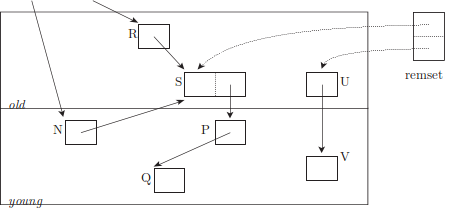
\includegraphics{figures/gen_1}
  \caption[Διαγενεαλογικοί δείκτες]
    {Διαγενεαλογικοί δείκτες. Η διατήρηση των ζωντανών αντικειμένων
     της νέας γενεάς χωρίς την εξερεύνηση όλου του σωρού, απαιτεί
     ένα μηχανισμό και μια δομή δεδομένων για την καταγραφή των
     αντικειμένων S και U που περιέχουν δείκτες προς αντικείμενα
     της νέας γενεάς.}
  \label{fig:gen_1} 
\end{figure}

Οι ρίζες μιας γενεάς πρέπει να ανακαλυφθούν πριν αυτή συλλεχθεί.
Οι ρίζες για μια γενεά δεν περιλαμβάνουν μόνο τους δείκτες που
βρίσκονται σε καταχωρητές, στη στοίβα και σε καθολικές μεταβλητές
αλλά και δείκτες προς αντικείμενα της γενεάς από αντικείμενα
που ζουν σε κάποια άλλη περιοχή του σωρού η οποία δε συλλέγεται
ταυτόχρονα με τη γενεά. Αυτές οι περιοχές τυπικά περιλαμβάνουν
τις παλαιότερες γενεές αλλά και περιοχές εκτός του γενεαλογικού
σωρού όπως χώροι που φιλοξενούν πολύ μεγάλα αντικείμενα και
χώροι που δε συλλέγονται ποτέ, όπως οι χώροι που αποθηκεύουν
αθάνατα αντικείμενα και πιθανώς κώδικα. Όπως έχουμε εξηγήσει,
οι διαγενεαλογικοί δείκτες δημιουργούνται είτε με την αρχικοποίηση
εγγραφών κατά τη δημιουργία των αντικειμένων, είτε από ενημερώσεις
πεδίων δεικτών αντικειμένων από τον τροποποιητή είτε τέλος κατά
την μετακίνηση αντικειμένων σε διαφορετικές γενεές. Γενικά, οι
δείκτες αυτοί πρέπει να εντοπίζονται τη στιγμή της δημιουργίας
τους και να καταγράφονται ώστε να μπορούν να χρησιμοποιηθούν
ως ρίζες κατά τη συλλογή μιας γενεάς. Κάθε δείκτης που πρέπει
να καταγράφεται καλείται συνήθως και \textbf{ενδιαφέρων δείκτης}.

\subsection{Σύνολα ανάμνησης}
Οι δομές δεδομένων που χρησιμοποιούνται για την καταγραφή διαγενεαλογικών
δεικτών ονομάζονται \textbf{σύνολα ανάμνησης}. Τα σύνολα ανάμνησης
καταγράφουν τη θέση προέλευσης διαφόρων δεικτών μεταξύ διαφορετικών
χώρων του σωρού. Καταγράφεται η προέλευση και όχι ο προορισμός
ενός δείκτη για δύο λόγους. Πρώτον, επιτρέπεται σε ένα μετακινούντα
συλλέκτη να ενημερώσει το πεδίο προέλευσης με τη νέα διεύθυνση
ενός αντικειμένου που έχει αντιγραφεί η προαχθεί. Δεύτερον ένα
πεδίο προέλευσης κάποιου δείκτη μπορεί να ενημερωθεί πολλές φορές
στο ανάμεσα σε δύο διαδοχικούς κύκλους συλλογής και έτσι αν ο
συλλέκτης θυμάται την προέλευση του δείκτη, εξασφαλίζεται πώς
αυτός επεξεργάζεται το πραγματικό αντικείμενο προς το οποίο
αναφέρεται ο δείκτης τη στιγμή της προέλευσης και όχι τα αντικείμενα
προορισμούς ενδιάμεσων παρωχημένων τιμών του αυτού. Επομένως το
σύνολο ανάμνησης για κάθε γενεά αποθηκεύει τις θέσεις εκείνες
στις οποίες βρίσκεται ένας πιθανόν ενδιαφέρων δείκτης προς κάποιο
αντικείμενο της γενεάς. Οι διάφορες υλοποιήσεις των συνόλων ανάμνησης 
διαφέρουν ως προς την ακρίβεια με την οποία καταγράφουν τέτοιες
θέσεις. Η επιλογή της ακρίβειας προσπαθεί να επιτύχει ένα
συμβιβασμό μεταξύ της επιβάρυνσης του τροποποιητή, του απαιτούμενου
χώρου αποθήκευσης των συνόλων ανάμνησης και το κόστος επεξεργασίας
τους από το συλλέκτη.

Εμφανώς είναι επιθυμητός ο εντοπισμός και η καταγραφή όσο το
δυνατόν λιγότερων δεικτών. Οι ενημερώσεις δεικτών από
το συλλέκτη κατά τη μετακίνηση αντικειμένων εντοπίζονται εύκολα.
Οι εγγραφές δεικτών από τον τροποποιητή μπορούν να ανιχνευθούν
από ένα φράγμα εγγραφής λογισμικού, το οποίο μπορεί να εισαχθεί
αυτόματα από το μεταγλωττιστή πριν από κάθε λειτουργία εγγραφής
ενός δείκτη. Αυτό βέβαια δεν είναι εφικτό αν ο μεταγλωττιστής
της γλώσσας είναι μη συνεργατικός. Στην περίπτωση αυτή, οι
θέσεις των λειτουργιών εγγραφής μπορούν συχνά να καθορισθούν
από το διαχειριστή εικονικής μνήμης του λειτουργικού συστήματος.

Η συχνότητα των ενημερώσεων δεικτών διαφέρει μεταξύ των
διαφορετικών γλωσσών προγραμματισμού και των υλοποιήσεων αυτών.
Ο Zorn εφαρμόζοντας στατική ανάλυση σε μια σουίτα προγραμμάτων
σε Lisp \cite{DBLP:conf/lfp/Zorn90}, υπολόγισε τη συχνότητα
των ενημερώσεων δεικτών από 13\% έως και 15\%, ενώ ο Appel
υπολόγισε μία χαμηλότερη στατική συχνότητα της τάξης του 3\% 
στη γλώσσα Lisp \cite{DBLP:journals/ipl/Appel87}, και μία
δυναμική συχνότητα χρόνου εκτέλεσης της τάξης του 1\% για
τη γλώσσα ML \cite{DBLP:journals/spe/Appel89a}. Οι Dieckmann
και H{\"o}lzle \cite{DBLP:conf/ecoop/DieckmannH99} βρήκαν
τέλος πώς τα προγράμματα σε γλώσσα Java μπορεί να διαφέρουν
σημαντικά ως προς τη συχνότητα των ενημερώσεων δεικτών
(το ποσοστό των προσβάσεων στο σωρό που αφορούσε αποθηκεύσεις
τιμών σε πεδία δείκτες κυμαινόταν από 6\% έως και 70\%).

Αν τα πλαίσια αυτά σαρώνονται ως μέρος του συνόλου ριζών σε
κάθε συλλογή, είναι δυνατή η ανακάλυψη των θέσεων τους που
περιέχουν δείκτες. Επιπλέον, αν ο μεταγλωττιστής μπορεί να
ταυτοποιήσει τις λειτουργίες εγγραφής στη στοίβα, τότε δε
χρειάζεται να τοποθετήσει φράγματα εγγραφής πριν από αυτές.
Επιπρόσθετα, πολλοί δείκτες αναφέρονται σε αντικείμενα της
ίδιας διαμέρισης. Παρότι οι αποθηκεύσεις πιθανώς εντοπίζονται,
οι δείκτες δεν είναι ενδιαφέροντες από γενεαλογική άποψη και
δε χρειάζεται να καταγραφούν.

Εάν επιβληθεί μια τάξη ως προς τη σειρά συλλογής των διαφόρων
γενεών, το πλήθος των διαγενεαλογικών δεικτών που πρέπει να
καταγραφούν μπορεί να μειωθεί ακόμη περισσότερο. Εξασφαλίζοντας
πώς οποτεδήποτε συλλέγεται μια γενεά συλλέγονται και όλες οι
νεότερες γενεές από αυτή, μόνο οι δείκτες από παλαιά αντικείμενα
προς νέα αντικείμενα πρέπει να καταγραφούν. Πολλές λειτουργίες
εγγραφής δεικτών αφορούν την αρχικοποίηση πεδίων αντικειμένων
που μόλις έχουν δημιουργηθεί. Εξ' ορισμού, οι δείκτες αυτοί
αναφέρονται σε γηραιότερα αντικείμενα. Δυστυχώς πολλές γλώσσες
διαχωρίζουν την εκχώρηση μνήμης για ένα αντικείμενο από την
αρχικοποίηση των πεδίων του τελευταίου, καθιστώντας δύσκολη τη
διάκριση των λειτουργιών εγγραφής δεικτών που δεν αφορούν
αρχικοποιήσεις και πιθανόν δημιουργούν δείκτες από μια παλαιά
γενεά προς μία νέα γενεά. Άλλες γλώσσες παρέχουν περισσότερη
υποστήριξη στο μεταγλωττιστή όσον αφορά την αναγνώριση των
λειτουργιών εγγραφής δεικτών που δε χρειάζονται κάποιο φράγμα
εγγραφής. Η πλειοψηφία των λειτουργιών εγγραφής δεικτών σε μία
αγνή οκνηρή γλώσσα συναρτησιακού προγραμματισμού όπως η Haskell
κάνει τους δείκτες να αναφέρονται σε γηραιότερα αντικείμενα.
Η γλώσσα ML απαιτεί από τον προγραμματιστή να σημειώσει ρητά
τις τροποποποιήσιμες μεταβλητές: οι λειτουργίες εγγραφής αυτών
των μεταβλητών είναι η μόνη πηγή δημιουργίας δεικτών από
αντικείμενα μιας παλαιάς γενεάς προς αντικείμενα μιας νέας
γενεάς. Το σκηνικό στις αντικειμενοστρεφείς γλώσσες προγραμματισμού
από την άλλη όπως για παράδειγμα στη Java είναι πιο πολύπλοκο.
Η φιλοσοφία προγραμματισμού εδώ βασίζεται στην ενημέρωση της
κατάστασης αντικειμένων, κάτι που οδηγεί φυσικά στη δημιουργία
περισσότερων δεικτών από αντικείμενα μιας νέας γενεάς προς
αντικείμενα μιας παλαιάς γενεάς.

Σε σωρούς με πολλαπλές ανεξάρτητα συλλεγόμενες γενεές απαιτείται
διαφορετική τεχνική φιλτραρίσματος δεικτών. Για παράδειγμα ένας
συλλέκτης μπορεί να εφαρμόσει ευριστικές για να αποφασίσει
ποιο χώρο θα συλλέξει, δίνοντας προτεραιότητα στους χώρους
με το μικρότερο πλήθος ζωντανών αντικειμένων. Στην περίπτωση
αυτή το φράγμα εγγραφής πρέπει να καταγράψει δείκτες και προς
τις δύο κατευθύνσεις. Καθώς αυτή η σχεδίαση αναμένεται να αυξήσει
το πλήθος των διαγενεαλογικών δεικτών προς καταγραφή, είναι
βέλτιστη για χρήση σε μια υλοποίηση όπου το μέγεθος του συνόλου
ανάμνησης είναι ανεξάρτητο του πλήθους των ενθυμούμενων
δεικτών.

\section{Διαχείριση χώρου}
Η νεότερη γενεά συνήθως διαχειρίζεται με αντιγραφή. Τα επιζώντα
αντικείμενα αντιγράφονται είτε σε ένα φρέσκο ημιχώρο στην
ίδια γενεά είτε σε μία παλαιότερη γενεά. Οι συλλογές των
νέων γενεών αναμένεται να είναι συχνές και σύντομες σε διάρκεια,
λαμβάνοντας υπόψη την ασθενή γενεαλογική υπόθεση. Από την άλλη
πλευρά, οι συλλογές των παλαιότερων γενεών αναμένεται να είναι
λιγότερες συχνές αλλά να διαρκούν πολύ, καθώς πρέπει μαζί με
αυτές πρέπει να συλλεγούν και οι νεότερες γενεές προκειμένου
να αποφευχθεί το κόστος χρήσης ενός φράγματος εγγραφής που
καταγράφει δείκτες και προς τις δύο κατευθύνσεις. Συνήθως
μια συλλογή της παλαιότερης γενεάς θα συλλέξει όλες τις περιοχές
του σωρού εκτός ίσως από την περιοχή όπου φιλοξενούνται αθάνατα
αντικείμενα (παρότι οι δείκτες της περιοχής αυτής αντιμετωπίζονται
ως ρίζες και ενδέχεται να ενημερωθούν). Μια πλήρης συλλογή του
σωρού δεν απαιτεί τη χρήση συνόλων ανάμνησης, εκτός ίσως για
τοποθεσίες της περιοχής αθάνατων αντικειμένων στην περίπτωση
που αυτή δε σαρώνεται.

Έχει προταθεί μία ευρεία γκάμα στρατηγικών διαχείρισης της
παλαιότερης γενεάς. Η συλλογή με αντιγραφή μεταξύ ημιχώρων
δεν είναι η καλύτερη επιλογή ειδικά αν λάβει κανείς υπόψη
πώς και η νεότερη γενεά συλλέγεται με την ίδια τεχνική: η
απαίτηση της συλλογής για την διατήρηση ενός εφεδρικού χώρου
αντιγραφής καταλήγει να δαπανά το μισό χώρο στο σωρό, κάτι
που έχει ως αποτέλεσμα την αύξηση της συχνότητας των συλλογών
όλων των γενεών. Επίσης τα μακρόβια αντικείμενα μετακινούνται
συνέχεια. Ο Blackburn κ.ά ισχυρίζονται \cite{DBLP:conf/icse/BlackburnCM04}
πώς η συλλογή με σήμανση και εκκαθάριση προσφέρει καλύτερη
χρησιμοποίηση του διαθέσιμου χώρου, ειδικά σε μικρούς σωρούς.
Το μειονέκτημα της συλλογής με σήμανση και εκκαθάριση, η οποία
δεν μετακινεί τα ζωντανά αντικείμενα, αφορά στη μείωση της
επίδοσης από την πιθανό κατακερματισμό. Η λύση είναι η προσθήκη
μιας φάσης συμπύκνωσης της παλαιάς γενεάς οποτεδήποτε ο
κατακερματισμός επηρεάζει δυσμενώς την επίδοση. Η συμπύκνωση
επίσης μπορεί να διαχειρισθεί τα μακρόβια αντικείμενα με
ειδικό τρόπο, όπως είδαμε στο κεφάλαιο~\ref{ch:mrkcmp}.

Οι γενεαλογικοί συλλέκτες σχεδόν πάντοτε διαχωρίζουν τις
γενεές τους φυσικά και όχι εικονικά. Αυτό απαιτεί τη διαχείριση
των νεότερων γενεών από συλλογή με αντιγραφή. Ένας προσαρμοστικός
συλλέκτης αντιγραφής σαν και αυτόν του Appel για παράδειγμα
συντηρητικά απαιτεί ο εφεδρικός χώρος αντιγραφής να έχει το
ίδιο μέγεθος με την περιοχή που συλλέγεται καθώς στην χειρότερη
περίπτωση όλα τα αντικείμενα μπορεί να επιβιώσουν. Στην πράξη
βέβαια τα περισσότερα αντικείμενα δεν επιβιώνουν από μια συλλογή
της νέας γενεάς.

Ο McGachey κ.ά. \cite{DBLP:conf/iwmm/McGacheyH06} ισχυρίζονται
πώς η χρησιμοποίηση του χώρου μπορεί να βελτιωθεί με τη διατήρηση
ενός μικρότερου μεγέθους εφεδρικού χώρου αντιγραφής και την
εναλλαγή μεταξύ συλλογής με αντιγραφή σε συλλογή με σήμανση και
συμπύκνωση οποτεδήποτε το μέγεθος του χώρου αυτού γίνει πολύ
μικρό. 

\section{Θέματα προς εξέταση}
Η γενεαλογική συλλογή σκουπιδιών έχει αποδειχθεί αποδοτική,
προσφέροντας σημαντικές βελτιώσεις επίδοσης για μια ευρεία
γκάμα εφαρμογών. Μειώνοντας το μέγεθος της νεότερης γενεάς
και επικεντρώνοντας τις προσπάθειες συλλογής σε αυτήν, οι
αναμενόμενοι χρόνοι παύσης μπορούν να ελαττωθούν σε τέτοιο
σημείο ώστε να περνούν σχεδόν απαρατήρητοι σε διάφορα περιβάλλοντα.
Η τεχνική της γενεαλογικής συλλογής σκουπιδιών μπορεί επίσης
να αυξήσει τη γενική ρυθμαπόδοση του συλλέκτη με δύο τρόπους.
Πρώτον, μειώνει τη συχνότητα επεξεργασίας των μακρόβιων αντικειμένων
και επομένως όχι μόνο μειώνει την υπολογιστική προσπάθεια αλλά
επιπλέον δίνει στα αντικείμενα αυτά περισσότερο χρόνο για να
πεθάνουν (και έτσι να μην χρειαστεί να εξιχνιαστούν οι υπογράφοι
των οποίων είναι ρίζες). Δεύτερον, οι γενεαλογικοί συλλέκτες
συνήθως εκχωρούν μνήμη για την αποθήκευση νέων αντικειμένων
σειριακά σε μία περιοχή βρεφοκομείου. Η σειριακή εκχώρηση έχει
ως αποτέλεσμα τη βελτίωση του ρυθμού αστοχιών κρυφής μνήμης
καθώς το μοτίβο πρόσβασης στη μνήμη είναι προβλέψιμο και
επιπλέον οι περισσότερες εγγραφές αφορούν τα νεότερα αντικείμενα.

Η γενεαλογική συλλογή σκουπιδιών ωστόσο δεν είναι πανάκεια.
Η αποδοτικότητά της εξαρτάται άμεσα από την κατανομή της διάρκειας
των αντικειμένων μιας εφαρμογής. Αν η μεγάλη πλειοψηφία των
αντικειμένων δεν πεθαίνει νέα, η γενεαλογική συλλογή σκουπιδιών
δεν είναι κατάλληλη.

Επιπλέον, η γενεαλογική συλλογή σκουπιδιών βελτιώνει μόνο
τους αναμενόμενους χρόνους παύσης. Τελικώς, ο συλλέκτης πρέπει
να συλλέξει όλο το σωρό και συνεπώς η γενεαλογική συλλογή από
μόνη της δεν μπορεί να επιλύσει το πρόβλημα της μείωσης του
χρόνου παύσης \textbf{χειρότερης περίπτωσης}, ο οποίος αυξάνεται
υπερβολικά πολύ σε μεγάλους σωρούς. Συνεπώς, η γενεαλογική
συλλογή σκουπιδιών δεν μπορεί να παράσχει τις απαιτούμενες εγγυήσεις
ενός σκληρού συστήματος πραγματικού χρόνου όπου οι προθεσμίες
πρέπει πάντοτε να τηρούνται.

Η υλοποίηση της συλλογής σκουπιδιών είναι απλούστερη αν υπάρχει
η δυνατότητα μετακίνησης αντικειμένων προς διάκριση των παλαιών
αντικειμένων από τα νέα. Ο φυσικός διαχωρισμός δεν προσφέρει
μόνο το πλεονέκτημα της τοπικότητας που συζητήθηκε παραπάνω,
αλλά επίσης πιο αποδοτικούς ελέγχους χώρου, οι οποίοι είναι
απαραίτητοι στο φράγμα εγγραφής αλλά και κατά την εξιχνίαση
της νεότερης γενεάς. Τα αντικείμενα πάντως μπορούν να διαχωρίζονται
με βάση την ηλικία τους και εικονικά, χρησιμοποιώντας πιθανώς
ένα bit στην επικεφαλίδα τους ή σε κάποιο bitmap.

Οι γενεαλογικοί συλλέκτες εγείρουν μια πληθώρα διαφορετικών
ερωτημάτων όσον αφορά τόσο τις επιλογές υλοποίησης όσο και
τις απαιτήσεις του τελικού χρήστη μιας εφαρμογής. Η υλοποίηση
γενεαλογικών συλλεκτών περιλαμβάνει πολύ περισσότερες σχεδιαστικές
επιλογές από την επιλογή του μεγέθους του σωρού.

Η πρώτη απόφαση υλοποίησης συνήθως αφορά το αν ο σωρός θα
οργανωθεί σε δύο ή περισσότερες γενεές. Η απάντηση εξαρτάται
πρωτίστως από τις κατανομές της διάρκειας ζωής των εφαρμογών
για τις οποίες ο συλλέκτης θα παρέχει υποστήριξη. Εάν ένα
σημαντικό ποσοστό των αντικειμένων αναμένεται να επιβιώσουν
από τη νεότερη γενεά αλλά να πεθάνουν σύντομα μετά την προαγωγή
τους, τότε ίσως αξίζει η προσθήκη ενδιάμεσων γενεών. Τα περισσότερα
συστήματα αυτόματης διαχείρισης μνήμης με γενεαλογική συλλογή
σκουπιδιών ωστόσο από προεπιλογή περιλαμβάνουν δύο γενεές και
μια αθάνατη γενεά. Η χρήση πολλαπλών γενεών προσπαθεί να λύσει
το πρόβλημα της πρόωρης προαγωγής αντικειμένων. Υπάρχουν και
άλλοι τρόποι επίλυσής του.

Αρχικά, ο ρυθμός προαγωγής εξαρτάται από το μέγεθος της νέας
γενεάς: μια μεγαλύτερη νέα γενεά προσφέρει περισσότερο χρόνο
σε ένα αντικείμενο για να πεθάνει. Μερικοί γενεαλογικοί συλλέκτες
επιτρέπουν στο χρήστη να ρυθμίσει ένα σταθερό μέγεθος για τη
νεότερη γενεά. Άλλοι πάλι επιτρέπουν στη νεότερη γενεά να
αυξάνεται δυναμικά μέχρις ότου καταλάβει όλο το σωρό (εκτός
από ήδη δεσμευμένες περιοχές, όπως η παλαιά γενεά και πιθανόν
μια εφεδρική περιοχή αντιγραφής). Οι πιο εξεζητημένοι συλλέκτες
σκουπιδιών πάντως μπορούν να μεταβάλλουν το μέγεθος της νεότερης
γενεάς προς ικανοποίηση συγκεκριμένων προδιαγραφών σχετικά
με τους χρόνους παύσης, λαμβάνοντας αποφάσεις για την αλλαγή
του μεγέθους με βάση την παρακολούθηση του προφίλ της συμπεριφοράς
του συλλέκτη.

Δεύτερον, η προαγωγή μπορεί να περιορισθεί ελέγχοντας την ηλικία
κατά την οποία τα αντικείμενα προάγονται. Η τεχνική της μαζικής
προαγωγής μεταφέρει όλους τους επιζώντες μιας συλλογής της νεότερης
γενεάς σε μια παλαιότερη γενεά. Αυτή η πολιτική προαγωγής έχει
μάλιστα την απλούστερη υλοποίηση, καθώς τα ενθυμούμενα σύνολα
για τη νεότερη γενεά μπορούν να παραμερισθούν μετά το πέρας
της συλλογής. Εναλλακτικά, ένας συλλέκτης μπορεί να απαιτεί
από ένα αντικείμενο να επιβιώσει περισσότερους του ενός κύκλων
συλλογής πριν το προάγει. Στην περίπτωση αυτή, είναι απαραίτητος
ένας μηχανισμός καταγραφής της ηλικίας των αντικειμένων. Αυτό
μπορεί να επιτευχθεί είτε με τη χρήση κάποιων bits από την
επικεφαλίδα των αντικειμένων, με τη διαίρεση μιας γενεάς σε
σε υποχώρους ο καθένας από τους οποίους φιλοξενεί αντικείμενα
διαφορετικής ηλικίας, είτε με συνδυασμό των δύο. Οι συνηθισμένες
διαμορφώσεις περιλαμβάνουν σχήματα οργανωμένα σε βήματα και
σχήματα που περιλαμβάνουν μια περιοχή εδέμ και ημιχώρους επιζώντων.

Τέλος, είναι πολλές φορές πιθανή η αποφυγή της υποχρέωσης
προαγωγής ορισμένων αντικειμένων. Πολλοί συλλέκτες σκουπιδιών
δεσμεύουν μια αθάνατη περιοχή για αντικείμενα που θα επιβιώσουν
μέχρι το τέλος του προγράμματος. Τα αντικείμενα αυτά συχνά μπορούν
να αναγνωρισθούν είτε κατά την υλοποίηση του συλλέκτη είτε από
το μεταγλωττιστή. Τέτοια αντικείμενα συνήθως περιλαμβάνουν
τις δομές δεδομένων του συλλέκτη καθώς αντικείμενα που αναπαριστούν
τον υπό εκτέλεση κώδικα.

Οι ρυθμοί προαγωγής μπορούν επίσης να επηρεάσουν το κόστος του
φράγματος εγγραφής καθώς επίσης και το μέγεθος των ενθυμούμενων
συνόλων. Υψηλότεροι ρυθμοί προαγωγής προκαλούν τη δημιουργία
περισσότερων διαγενεαλογικών δεικτών που πρέπει να καταγραφούν.
Εάν αυτό επηρεάζει ή όχι την απόδοση των φραγμάτων εγγραφής
εξαρτάται από την υλοποίηση.

Η συχνότητα κλήσης των φραγμάτων εγγραφής εξαρτάται επίσης
από το αν οι διαφορετικές γενεές μπορούν να συλλεχθούν ανεξάρτητα.
Η ανεξάρτητη συλλογή των γενεών απαιτεί την καταγραφή όλων
των διαγενεαλογικών δεικτών. Η εγκατάλειψη αυτής της ευελιξίας
σημαίνει πώς την ταυτόχρονη συλλογή όλων των νεότερων γενεών
οποτεδήποτε συλλέγεται η παλαιότερη γενεά και επιτρέπει την
καταγραφή μόνο των δεικτών με προέλευση κάποια παλαιότερη
γενεά και προορισμό κάποια νεότερη γενεά (οι οποίοι αναμένεται
να είναι σημαντικά λιγότεροι σε πλήθος). Σημειώνοντας το
αντικείμενο και όχι το συγκεκριμένο πεδίο αυτού ως πιθανή
προέλευση ενός διαγενεαλογικού δείκτη, το κόστος σε χώρο για
την αποθήκευση των συνόλων ανάμνησης μπορεί να μειωθεί.

Οι διαφορετικοί μηχανισμοί που χρησιμοποιεί ο τροποποιητής για
την καταγραφή των πιθανών προελεύσεων διαγενεαλογικών δεικτών
επηρεάζουν το κόστος της συλλογής. Παρότι μηχανισμοί λιγότερο
ακριβείς μπορεί να μειώσουν το κόστος του φράγματος εγγραφής,
αυτοί μπορεί να αυξήσουν το φορτίο εργασίας του συλλέκτη.
Η καταγραφή του πεδίου προέλευσης με χρήση σειριακών απομονωτών
αποθήκευσης είναι ο πιο ακριβής μηχανισμός παρότι ένας απομονωτής
ενδέχεται να περιλαμβάνει κάποιες καταχωρίσεις εις διπλούν.
Η καταγραφή του αντικειμένου προέλευσης από την άλλη πλευρά
απαιτεί τη σάρωση του αντικειμένου για την εύρεση διαγενεαλογικών
δεικτών.

\end{greek}

\begin{greek}

\chapter{Παράλληλη συλλογή σκουπιδιών}\label{ch:par}
Μέχρι τώρα έχουμε υποθέσει πώς, ενώ ο τροποποιητής μπορεί να
είναι πολυνηματικός, ο συλλέκτης είναι μονονηματικός. Η υπόθεση
αυτή οδηγεί σε φτωχή εκμετάλλευση των πόρων ενός σύγχρονου
πολυπύρηνου μηχανήματος. Στο παρόν κεφάλαιο εξετάζουμε πώς
μπορεί να παραλληλοποιηθεί ο συλλέκτης, υποθέτοντας ακόμα πώς
κανένα από τα νήματα του τροποποιητή δεν εκτελείται ενώ
πραγματοποιείται συλλογή σκουπιδιών και πώς αυτή ολοκληρώνεται
πριν αυτά συνεχίσουν την εκτέλεσή τους. Ένας προφανής τρόπος
προκειμένου να μειωθεί ο χρόνος παύσης των νημάτων τροποποιητών
είναι οι πυρήνες να συνεργαστούν κατά τη συλλογή σκουπιδιών
(και ενώ τα νήματα του τροποποιητή είναι σταματημένα). Η 
\textbf{παράλληλη συλλογή σκουπιδιών} είναι το αντικείμενο
αυτού του κεφαλαίου. Πιο συγκεκριμένα θα εξετάσουμε πώς μπορούν
να παραλληλοποιηθούν οι τέσσερις βασικές διαδικασίες της συλλογής
με εξιχνίαση: σήμανση, εκκαθάριση, αντιγραφή και συμπύκνωση.

\begin{figure}[H]
  \centering
  \begin{subfigure}{1.0\textwidth}
    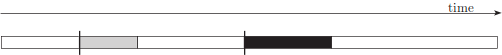
\includegraphics{figures/par_1a}
    \caption
      {Συλλογή με παύση του κόσμου, μονονηματικός τροποποιητής, 
       μονονηματικός συλλέκτης.}
  \end{subfigure}

  \begin{subfigure}[b]{1.0\textwidth}
    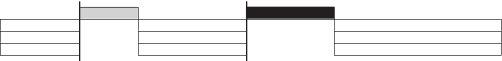
\includegraphics{figures/par_1b}
    \caption
      {Συλλογή με παύση του κόσμου, πολυνηματικός τροποποιητής,
       μονονηματικός συλλέκτης.}
  \end{subfigure}
  
  \begin{subfigure}[b]{1.0\textwidth}
    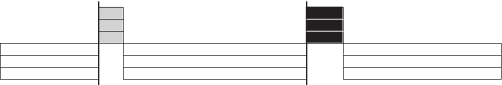
\includegraphics{figures/par_1c}
    \caption
      {Συλλογή με παύση του κόσμου, πολυνηματικός τροποποιητής,
       πολυνηματικός συλλέκτης.}
  \end{subfigure}
  
  \caption
    [Συλλογή σκουπιδιών με παύση του κόσμου: κάθε μπάρα αναπαριστά
     την εκτέλεση σε έναν επεξεργαστή.]
    {Συλλογή σκουπιδιών με παύση του κόσμου: κάθε μπάρα αναπαριστά
     την εκτέλεση σε έναν επεξεργαστή. Οι χρωματισμένες περιοχές
     αναπαριστούν διαφορετικούς κύκλους συλλογής σκουπιδιών.}
  \label{fig:par_1}
\end{figure}

\section{Υπάρχει επαρκής δουλειά προς παραλληλοποίηση;}
Όπως και κατά την παραλληλοποίηση του αλγορίθμου οποιουδήποτε
προβλήματος, η πρώτη απαίτηση αφορά στην εξασφάλιση του ότι
το φορτίο εργασίας είναι αρκετά μεγάλο ώστε η παραλληλοποίηση
να αξίζει τον κόπο. Αναπόφευκτα, η παράλληλη συλλογή σκουπιδιών
απαιτεί κάποια μορφή συγχρονισμού των νημάτων συλλεκτών με το
συγχρονισμό αυτό να κοστίζει. Ο συγχρονισμός αυτός μπορεί να
επιτευχθεί με τη χρήση είτε κλειδωμάτων είτε ατομικών πρωταρχικών
λειτουργιών υλικού όπως για παράδειγμα της \textproc{CompareAndSwap}
και την προσεκτική σχεδίαση βοηθητικών δομών δεδομένων. Προκύπτει
λοιπόν το ερώτημα αν το φορτίο εργασίας της συλλογής σκουπιδιών
επαρκεί ώστε το κέρδος από την παραλληλοποίηση να υπερκερνά το
κόστος του συγχρονισμού.

Aς υποθέσουμε για παράδειγμα, πώς ένας συλλέκτης με σήμανση
και εκκαθάριση θα πρέπει να σημάνει μία απλή συνδεδεμένη λίστα:
σε κάθε βήμα, η στοίβα σήμανσης θα περιέχει μόνο ένα αντικείμενο,
τον επόμενο κόμβο προς εξέταση. Στην περίπτωση αυτή, μόνο ένα από
τα νήματα συλλέκτες θα δουλεύει, ενώ τα υπόλοιπα θα είναι αδρανή,
περιμένοντας για δουλειά. Ο Siebert \cite{DBLP:conf/iwmm/Siebert08}
αποδεικνύει πώς ο αριθμός φορών $n$ που ένας επεξεργαστής μένει
αδρανής κατά τη διάρκεια μιας παράλληλης σήμανσης σε ένα σύστημα
με $p$ επεξεργαστές φράσσεται από το μέγιστο βάθος των προσβάσιμων
αντικειμένων $o$:

\begin{equation}
  n \leq (p-1) \cdot \max_{o \in reachable}{depth(o)}
  \label{eq:par_1}
\end{equation}

Η ανίσωση αυτή πάντως βασίζεται στην όχι ρεαλιστική υπόθεση
πώς όλα τα βήματα σήμανσης διαρκούν το ίδιο, κάτι που δεν ισχύει
καθώς οι χρόνοι διαφέρουν ανάλογα με το μέγεθος του αντικειμένου.
Στις περισσότερες γλώσσες προγραμματισμού πάντως η μεγάλη πλειοψηφία
των αντικειμένων είναι μικρά (περιέχουν λίγους δείκτες).

Μελέτες πάντως έχουν δείξει πώς οι τυπικές εφαρμογές περιλαμβάνουν
μια ευρεία ποικιλία από πλούσιες σε δείκτες δομές δεδομένων.
Για παράδειγμα, η εξιχνίαση μιας δενδροειδούς δομής δεδομένων
θα παράγει περισσότερες μονάδες εργασίας από όσες θα καταναλώνει
μέχρις ότου η εξερεύνηση φθάσει στα φύλλα.

\section{Εξισορρόπηση φορτίου}
Μια άλλη απαίτηση από την παράλληλη συλλογή σκουπιδιών είναι
το φορτίο της συλλογής να κατανεμηθεί με τέτοιο τρόπο ώστε να
ελαχιστοποιηθεί η ανάγκη για συντονισμό και όλοι οι επεξεργαστές
να είναι απασχολημένοι ταυτόχρονα. Ο Endo κ.ά \cite{DBLP:conf/sc/EndoTY97}
διαπιστώνουν πώς χωρίς κάποιο μηχανισμό για \textbf{εξισορρόπηση
φορτίου}, μια απλοϊκή παραλληλοποίηση μπορεί να οδηγήσει σε
πολύ μικρή επιτάχυνση σε πολυεπεξεργαστικά συστήματα.

Δυστυχώς, ο στόχος της ομοιόμορφης κατανομής υπολογιστικού φορτίου
και της ελαχιστοποίησης του απαιτούμενου συντονισμού αλληλοσυγκρούονται.
Ο στατικός διαμοιρασμός του υπολογιστικού φόρτου δεν είναι
πάντα ο καλύτερος. Για παράδειγμα, έστω ένας παράλληλος συλλέκτης
με σήμανση και συμπύκνωση σε σύστημα N επεξεργαστών. Αν ο σωρός
διαιρεθεί σε $N$ τμήματα, και ο κάθε επεξεργαστής αναλάβει την
επιδιόρθωση των δεικτών στο δικό του τμήμα, τότε, αν ο αριθμός
των αντικειμένων και των δεικτών που αυτά περιέχουν ποικίλλει
πολύ από τμήμα σε τμήμα, κάποιοι επεξεργαστές θα δουλεύουν
περισσότερο από άλλους. Εξίσου σημαντική με την εξισορρόπηση
του υπολογιστικού φορτίου ανάμεσα στους επεξεργαστές είναι
και η εξισορρόπηση άλλων πόρων. Σε μία παράλληλη υλοποίηση
του αλγόριθμου αντιγραφής του Baker \cite{DBLP:journals/cacm/Baker78},
ο Halstead \cite{DBLP:conf/lfp/Halstead84, DBLP:journals/toplas/Halstead85}
ανέθεσε σε κάθε επεξεργαστή το δικό του χώρο-προς και χώρο-από.
Δυστυχώς, αυτός ο στατικός διαμοιρασμός συχνά οδηγούσε σε μία
κατάσταση όπου ένας επεξεργαστής εξαντλούσε το δικό του χώρο-από
και ενώ υπήρχε χώρος στους χώρους-από των υπολοίπων επεξεργαστών.

Ένας \textbf{δυναμικός διαμοιρασμός} είναι περισσότερο κατάλληλος
προκειμένου η δουλειά να μοιραστεί σχεδόν ομοιόμορφα. Ας θεωρήσουμε
για παράδειγμα ένα συλλέκτη με σήμανση και εκκαθάριση: αφού έχει
ολοκληρωθεί η σήμανση των ζωντανών αντικειμένων, ο σωρός διαχωρίζεται
σε $Ν$ τμήματα, τα οποία έχουν παρόμοιο πλήθος ζωντανών αντικειμένων
και δεικτών. Στη συνέχεια, οι επεξεργαστές συμπυκνώνουν παράλληλα
ο καθένας το δικό του τμήμα του σωρού. Αυτή είναι ακριβώς η
προσέγγιση των Flood κ.ά \cite{DBLP:conf/jvm/FloodDSZ01}.

Συχνά η εξαρχής εκτίμηση εργασίας για την καλύτερη διαίρεσή της
δεν είναι εφικτή. Σε αυτήν την περίπτωση η συνηθισμένη λύση
είναι να \textbf{υπερ-διαμερίζεται} η συνολική εργασία ούτως
ώστε να υπάρχουν περισσότερα τμήματα εργασίας από ότι επεξεργαστές
ή νήματα και οι επεξεργαστές (ή τα νήματα) να τίθενται σε
ανταγωνισμό για την απόκτηση τους. Βασικό πλεονέκτημα της τεχνικής
αυτής αποτελεί το γεγονός πώς είναι ανθεκτική σε αλλαγές του
διαθέσιμου πλήθους επεξεργαστών στο συλλέκτη (π.χ. λόγω της
επιβάρυνσης από άλλες διεργασίες που εκτελούνται παράλληλα), καθώς
οι μικρότερες μονάδες εργασίες ανταλλάσσονται πιο εύκολα.

Απλοποιούμε τους αλγορίθμους που θα παρουσιάσουμε αργότερα εστιάζοντας
την προσοχή μας στις τρεις βασικές υπο-εργασίες της απόκτησης,
εκτέλεσης και δημιουργίας δουλειάς συλλογής. Θεωρούμε λοιπόν πώς,
στις περισσότερες περιπτώσεις, κάθε νήμα του συλλέκτη εκτελεί
τον ακόλουθο βρόχο:

\begin{algorithm}
  \caption{Παράλληλη συλλογή σκουπιδιών}
  \label{alg:par_1}
  \begin{algorithmic}[1]
    \Procedure{run}{\null}
      \While{\textbf{not} \Call{terminated}{\null}}
        \State \Call{acquireWork}{\null}
        \State \Call{performWork}{\null}
        \State \Call{generateWork}{\null}
      \EndWhile
    \EndProcedure
  \end{algorithmic}
\end{algorithm}

\section{Συγχρονισμός}
Εκ πρώτης όψεως ίσως φαίνεται πώς η βέλτιστη στρατηγική
εξισορρόπησης του φορτίου εργασίας είναι η διαίρεση του στις
ελάχιστες δυνατές υποεργασίες, όπως για παράδειγμα η σήμανση
ή η αντιγραφή ενός μόνο αντικειμένου. Παρότι η λύση αυτή πετυχαίνει
τέλειο διαμοιρασμό εργασίας ανάμεσα στους επεξεργαστές, το
κόστος που επιβάλλει ο συντονισμός των τελευταίων την καθιστά
απαγορευτική. Ο συγχρονισμός απαιτείται τόσο για την εξασφάλιση
της ορθότητας όσο και για την αποφυγή της επανάληψης, ή
τουλάχιστον ελαχιστοποίησης της εκτέλεσης ορισμένων μονάδων
εργασίας περισσότερες από μια φορές.

Η επίτευξη συγχρονισμού μεταξύ των νημάτων συλλεκτών κοστίζει
σε χρόνο και σε χώρο. Οι μηχανισμοί που εξασφαλίζουν αποκλειστικότητα
πρόσβασης χρησιμοποιούν μεταξύ άλλων κλειδώματα ή δομές
δεδομένων χωρίς αναμονή. Οι καλώς σχεδιασμένοι αλγόριθμοι
ελαχιστοποιούν τις περιπτώσεις όπου απαιτούνται ενέργειες
συγχρονισμού, παρέχοντας για παράδειγμα σε κάθε νήμα ιδιωτικές
τοπικές δομές δεδομένων. Σε μερικές περιπτώσεις πάντως η
μη αποκλειστική πρόσβαση δεν είναι απαραίτητη για την εξασφάλιση
της ορθότητας και έτσι κάποιες ενέργειες συγχρονισμού μπορούν
να παραληφθούν.

Οι μοντέρνες υλοποιήσεις παράλληλης συλλογής σκουπιδιών συνήθως
θέτουν να νήματα εργασίας σε ανταγωνισμό για την απόκτηση
μονάδων εργασίας, τις οποίες στη συνέχεια εκτελούν χωρίς περαιτέρω
συγχρονισμό. Οι μονάδες εργασίας οργανώνονται είτε ως τοπικές
στοίβες σήμανσης, είτε ως ξεχωριστές περιοχές του σωρού προς
σάρωση είτε ως καθολικές δεξαμενές. Οι βοηθητικές δομές δεδομένων
για την οργάνωση των μονάδων εργασίας επιβάλλουν ένα κόστος σε
χώρο για την αποθήκευση των μεταδεδομένων τους, το οποίο όμως
τείνει να είναι μικρό.

\section{Ταξινόμηση}
Στο υπόλοιπο του κεφαλαίου παρουσιάζουμε ειδικές λύσεις στο
πρόβλημα της παραλληλοποίησης της σήμανσης, της εκκαθάρισης,
της αντιγραφής και της συμπύκνωσης. Σε όλες τις περιπτώσεις
ενδιαφερόμαστε στο πώς οι αλγόριθμοι αποκτούν, εκτελούν και
παράγουν εργασίες. Η σχεδίαση και η υλοποίηση αυτών των τριών
δραστηριοτήτων καθορίζει τον απαιτούμενο συγχρονισμό, τη
διακριτότητα των φορτίων εργασίας των νημάτων καθώς επίσης
και πώς αυτά τα φορτία διαμοιράζονται ομοιόμορφα μεταξύ
επεξεργαστών.

Οι αλγόριθμοι παράλληλης συλλογής σκουπιδιών μπορούν να
κατηγοριοποιηθούν με βάση το αν στο επίκεντρο της σχεδίασης
είναι ο επεξεργαστής ή η μνήμη. Οι αλγόριθμοι της πρώτης
κατηγορίας τείνουν να επιτρέπουν στα νήματα να αποκτούν κβάντα
εργασίας μεταβλητού μεγέθους, συνήθως κλέβοντας εργασία
από άλλα νήματα. Λίγη έως και καθόλου σημασία δίνεται στην
τοποθεσία των αντικειμένων στη μνήμη, παρότι η τοπικότητα
επηρεάζει την επίδοση ακόμη και σε μονοπύρηνες αρχιτεκτονικές.
Οι αλγόριθμοι της δεύτερης κατηγορίας από την άλλη πλευρά
λαμβάνουν περισσότερο υπόψην τους τη θέση των αντικειμένων
στη μνήμη. Συνήθως λειτουργούν σε συνεχόμενα μπλοκ μνήμης
σωρού και αποκτούν/κατεθέτουν εργασία από/προς μοιραζόμενες
δεξαμενές.

Τέλος, εξετάζουμε τον τερματισμό της παράλληλης συλλογής
σκουπιδιών. Συνήθως, απλώς η εξέταση του κατά πόσο μια δεξαμενή
εργασίας είναι κενή δεν επαρκεί, καθώς ένα ενεργό νήμα μπορεί
να ετοιμάζεται να καταθέσει καινούριες μονάδες εργασίας σε αυτή.

\section{Παράλληλη Σήμανση}
Η φάση της σήμανσης, σε αντίθεση με τις φάσεις της εκκαθάρισης
και της συμπύκνωσης δεν είναι εγγενώς παραλληλοποιήσιμη.

\subsection{Κλοπή εργασιών}
Οι Endo κ.ά \cite{DBLP:conf/sc/EndoTY97}, Flood κ.ά \cite{DBLP:conf/jvm/FloodDSZ01}
καθώς και ο Siebert \cite{DBLP:conf/iwmm/Siebert10} χρησιμοποιούν 
\textbf{κλοπή εργασίας (work stealing)} για την εξισορρόπηση
του υπολογιστικού φόρτου. Οποτεδήποτε ένα νήμα ξεμένει από
δουλειά σήμανσης, κλέβει δουλειά που ανήκει σε ένα άλλο νήμα.
Σε μία παράλληλη υλοποίηση του συντηρητικού συλλέκτη των Boehm
και Weiser \cite{DBLP:journals/spe/BoehmW88}, ο Endo κ.ά παρέχουν
σε κάθε νήμα σήμανσης την δική του τοπική στοίβα σήμανσης καθώς
επίσης και μία \textbf{κλεπτόμενη ουρά εργασιών}. Περιοδικά,
κάθε νήμα ελέγχει την κλεπτόμενη ουρά εργασιών του και αν αυτή
είναι άδεια, μεταφέρει όλη την ιδιωτική στοίβα σήμανσης του (εκτός
των τοπικών ριζών) στην ουρά. Ένα αδρανές νήμα αποκτά έργο σήμανσης
ελέγχοντας αρχικά την δική του κλεπτόμενη ουρά και στη συνέχεια
τις κλεπτόμενες ουρές των άλλων νημάτων. Όταν ένα νήμα βρει μια
μη κενή κλεπτόμενη ουρά, κλέβει τις μισές καταχωρίσεις αυτής
και τις μεταφέρει στην ιδιωτική του στοίβα σήμανσης. Καθώς πολλά
νήματα προσπαθούν να κλέψουν δουλειά ταυτόχρονα, οι κλεπτόμενες
ουρές εργασιών προστατεύονται με κλειδώματα. 

Κάθε παράλληλος συλλέκτης οφείλει να είναι ιδιαίτερα προσεκτικός
όσον αφορά την ενημέρωση bitmap σήμανσης και την επεξεργασία
μεγάλων πινάκων. Τα bits μιας λέξης σε ένα bitmap σήμανσης πρέπει
να ενημερώνονται ατομικά. Αντί να κλειδώνουν ολόκληρη τη λέξη
όταν ελέγχουν ένα bit, ο Endo κ.ά χρησιμοποιούν μια απλή φόρτωση
για τον έλεγχο του bit και μόνον αν αυτό έχει την τιμή 0, επιχειρούν
ατομικά να εγγράψουν την τιμή 1 σε αυτό, προσπαθώντας εκ νέου,
αν η εγγραφή αποτύχει. Αντίθετα, συλλέκτες σαν αυτόν του Flood
κ.ά \cite{DBLP:conf/jvm/FloodDSZ01}, οι οποίοι αποθηκεύουν το
bit σήμανσης στην επικεφαλίδα του αντικειμένου μπορούν να
πραγματοποιούν σημάνσεις χωρίς τη χρήση ατομικών λειτουργιών.

Η επεξεργασία μεγάλων πινάκων αποτελεί πηγή πολλών προβλημάτων.
Για παράδειγμα, οι Boehn και Weiser \cite{DBLP:journals/spe/BoehmW88}
επιχειρούν να αποτρέψουν την υπερχείλιση της στοίβας σήμανσης
ωθώντας μεγάλα αντικείμενα σε τμήματα των 128 λέξεων. Παρόμοια,
και προκειμένου να βελτιώσουν την εξισορρόπηση φορτίου, ο Endo
κ.ά διαιρούν ένα μεγάλο αντικείμενο σε κομμάτια των 512 λέξεων 
πριν το τελευταίο εισαχθεί σε κάποια στοίβα σήμανσης ή κλεπτόμενη 
ουρά.

Ο παράλληλος γενεαλογικός συλλέκτης των Flood κ.ά \cite{DBLP:conf/jvm/FloodDSZ01}
διαχειρίζεται τη νέα γενιά με αντιγραφή και την παλαιά με
σήμανση και συμπύκνωση. Σε αυτήν την ενότητα εξετάζουμε μόνο
την παράλληλη σήμανση. Ενώ o Endo κ.ά χρησιμοποιούν μία στοίβα
και μια ουρά ανά επεξεργαστή, ο Flood κ.ά χρησιμοποιούν μία
\textbf{διπλά τερματισμένη ουρά (deque)} ανά νήμα σήμανσης.
Ο αλγόριθμος τους για κλοπή εργασίας δε χρησιμοποιεί κλειδώματα,
επιτρέπει το διαμοιρασμό εργασίας σε επίπεδο αντικειμένων και
βασίζεται στην ιδέα των Dimpsey κ.ά \cite{DBLP:journals/ibmsj/DimpseyAK00}.

\begin{algorithm}
  \caption{Παράλληλη σήμανση-εκκαθάριση: παράλληλη σήμανση με κλοπή εργασίας (Endo κ.ά)}
  \label{alg:par1}
  \begin{algorithmic}[1]
    \State \textbf{shared} \; stealableWorkQueue[N] \Comment{one per thread}
    \State $me \gets myThreadId$
    \Statex
    \Procedure{acquireWork}{\null}
      \If{\textbf{not} \Call{isEmpty}{$myMarkStack$}}
        \State \Return{\null}
      \EndIf
      \State \Call{lock}{$stealableWorkQueue[me]$}
      \State $n \gets$ \Call{size}{$stealableWorkQueue[me]$}/2 \Comment{grab half of my stealable work queue}
      \State \Call{transfer}{$stealableWorkQueue[me]$, $n$, $myMarkStack$}
      \State \Call{unlock}{$stealableWorkQueue[me]$}
      \If{\Call{isEmpty}{$myMarkStack$}}
        \ForAll{$j \; \textbf{in} \; Threads$}
          \If{\textbf{not} \Call{locked}{$stealableWorkQueue[j]$}}
            \If{\Call{lock}{$stealableWorkQueue[j]$}}
              \State $n \gets$ \Call{size}{$stealableWorkQueue[me]$}/2 \Comment{grab half of his stealable work queue}
              \State \Call{transfer}{$stealableWorkQueue[j]$, $n$, $myMarkStack$}
              \State \Call{unlock}{$stealableWorkQueue[j]$}
              \State \Return{\null}
            \EndIf
          \EndIf
        \EndFor
      \EndIf 
    \EndProcedure
    \Statex  
    \Procedure{performWork}{\null}
      \While{\Call{pop}{$myMarkStack$, $ref$}}
        \ForAll{$fld \; \textbf{in} \; Pointers(ref)$}
          \State $child \gets *fld$
          \If{$child \neq \textbf{null} \; \textbf{and} \; \textbf{not}$ \Call{isMarked}{$child$}}
            \State \Call{setMarked}{$child$}
            \State \Call{push}{$myMarkStack$, $child$}
          \EndIf
        \EndFor
      \EndWhile
    \EndProcedure
    \Statex
    \Procedure{generateWork}{\null} \Comment{transfer all my stack to my stealable work queue}
      \If{\Call{isEmpty}{$stealableWorkQueue[me]$}}
        \State $n \gets$ \Call{size}{$myMarkStack$}
        \State \Call{lock}{$myStealableWorkQueue[me]$}
        \State \Call{transfer}{$myMarkStack$, $n$, $stealableWorkQueue[me]$}
        \State \Call{unlock}{$myStealableWorkQueue[me]$}
      \EndIf
    \EndProcedure
  \end{algorithmic}
\end{algorithm}

\begin{algorithm}
  \caption{Παράλληλη σήμανση με χρήση bitmap}
  \label{alg:par2}
  \begin{algorithmic}[1]
    \Procedure{setMarked}{$ref$}
      \State $oldByte \gets$ \Call{markByte}{$ref$}
      \State $bitPosition \gets$ \Call{markBit}{$ref$}
      \State \textbf{loop}
      \Loop
        \If{\Call{isMarked}{$oldByte$, $bitPosition$}}
          \State \Return{\null}
        \EndIf
        \State $newByte \gets$ \Call{mark}{$oldByte$, $bitPosition$}
        \If{\Call{compareAndSet}{$\&markByte(ref)$, $oldByte$, $newByte$}}
          \State \Return{\null}
        \EndIf
      \EndLoop
    \EndProcedure
  \end{algorithmic}
\end{algorithm}

Ένα νήμα αντιμετωπίζει το κάτω μέρος της διπλά συνδεδεμένης ουράς
του ως στοίβα σήμανσης: η λειτουργία ώθησης δεν απαιτεί συγχρονισμό
ενώ η λειτουργία εξώθησης απαιτεί συγχρονισμό μόνο όταν η διπλά
συνδεδεμένη ουρά αποτελείται από ένα μόνο στοιχείο. Νήματα χωρίς
εργασία κλέβουν ένα αντικείμενο από το πάνω μέρος των διπλά συνδεδεμένων
ουρών των άλλων νημάτων με χρήση της συγχρονισμένης λειτουργίας
\textproc{remove}. Ένα βασικό πλεονέκτημα αυτής της σχεδίασης
για κλοπή εργασιών είναι πώς ο ακριβός μηχανισμός συγχρονισμού
ενεργοποιείται μόνο όταν υπάρχει ανάγκη για εξισορρόπηση εργασιών.

Οι διπλά συνδεδεμένες ουρές έχουν σταθερό μέγεθος ώστε να αποφεύγεται
η ανάγκη για εκχώρηση μνήμης στη διάρκεια μιας συλλογής. Καθώς
η προσέγγιση αυτή διακινδυνεύει την εμφάνιση υπερχείλισης ο
Flood κ.ά χρησιμοποιούν ένα καθολικό σύνολο υπερχείλισης το
οποίο επιφέρει μία μικρή επιβάρυνση ανά κλάση. Η δομή κάθε
κλάσης Java κρατάει μία λίστα όλων των αντικειμένων υπερχείλισης
της κλάσης, τα οποία συνδέονται μεταξύ τους μέσω του πεδίου
τύπου τους. Η υπερχείλιση χειρίζεται ως εξής: οποτεδήποτε η
ώθηση ενός αντικειμένου στο κάτω μέρος της διπλά-τερματισμένης
ουράς θα προκαλέσει υπερχείλιση, τα μισά αντικείμενα του κάτω
μέρους μετακινούνται στα αντίστοιχα σύνολα υπερχείλισης των
κλάσεων τους. Αντίστροφα, νήματα σήμανσης που βρίσκονται σε
αναζήτηση εργασίας επιχειρούν να γεμίσουν τη μισή διπλά-τερματισμένη
ουρά τους εξετάζοντας πρώτα το σύνολο υπερχείλισης και έπειτα
τις διπλά-τερματισμένες ουρές των άλλων νημάτων σήμανσης.

Ο Siebert \cite{DBLP:conf/iwmm/Siebert10} επίσης χρησιμοποιεί
κλοπή εργασιών για μια παράλληλη και ταυτόχρονη υλοποίηση της
εικονικής μηχανής Jamaica για τη γλώσσα Java. Τα αντικείμενα
διασπώνται σε συνδεδεμένα μπλοκ για να φραγεί ο χρόνος κάθε
βήματος σήμανσης και συνεπώς ο συλλέκτης δουλεύει με μπλοκ και
όχι με αντικείμενα. Μια συνέπεια του παραπάνω γεγονότος είναι
πώς τα χρώματα συσχετίζονται με μπλοκ. Όπως θα δούμε στο κεφάλαιο
\ref{ch:conc}, νήματα τροποποιητές και νήματα συλλέκτες
που εκτελούνται ταυτόχρονα ενδέχεται να χρειαστεί να προσπελάσουν
λίστες από γκρι μπλοκ. Για να αποφύγει την ανάγκη συγχρονισμού
τέτοιων προσπελάσεων, η εικονική μηχανή Jamaica χρησιμοποιεί
τοπικές λίστες γκρι μπλοκ ανά επεξεργαστή. Το κόστος αυτής της
σχεδίασης είναι πώς το χρώμα ενός μπλοκ αναπαρίσταται από μία
ολόκληρη λέξη και όχι ορισμένα bits. Ένα νήμα σημαίνει ένα
μπλοκ με γκρι χρώμα χρησιμοποιώντας μια λειτουργία \textproc{CompareAndSwap}
για να το συνδέσει μέσω του χρώματος του στην \textbf{τοπική}
γκρι λίστα του επεξεργαστή στον οποίο εκτελείται. Για την
εξισορρόπηση φορτίου, ένα νήμα χωρίς εργασία επιχειρεί να
κλέψει όλη τη γκρι λίστα μπλοκ ενός άλλου νήματος. Για να
αποτραπεί η επεξεργασία ενός μπλοκ από δύο ή περισσότερα νήματα
ταυτόχρονα, ένα νήμα σημαίνεται ως \textbf{ανθρακί} κατά τη
διάρκεια της επεξεργασίας του σε κάποιο στάδιο σήμανσης. Τα
νήματα κλέφτες επίσης κλέβουν επιχειρώντας να αλλάξουν το χρώμα
της κεφαλής μιας γκρι λίστας ενός άλλου επεξεργαστή σε ανθρακί.
Αυτός ο μηχανισμός είναι ιδανικός στην περίπτωση όπου το νήμα
θύμα δεν πραγματοποιεί εργασίες συλλογής εκτός ίσως από την
πρόσθεση μπλοκ στη γκρι λίστα του ενώ εκτελεί φράγματα εγγραφής.
Αυτό είναι ρεαλιστικό σενάριο για έναν ταυτόχρονο, πραγματικού
χρόνου συλλέκτη.

\subsection{Τερματισμός με κλοπή εργασιών}
Τελικώς, ο συλλέκτης θα πρέπει να είναι σε θέση να καθορίσει
το τέλος μιας φάσης, δηλαδή πότε όλα τα συνεργαζόμενα νήματα
έχουν ολοκληρώσει τις εργασίες τους. Ο Endo κ.ά \cite{DBLP:conf/sc/EndoTY97}
προσπάθησαν αρχικώς να ανιχνεύσουν τον τερματισμό με τη χρήση
ενός απλού καθολικού μετρητή των άδειων στοιβών σήμανσης και
των άδειων κλεπτόμενων ουρών σήμανσης. Ωστόσο ο ανταγωνισμός
για την ατομική ενημέρωση του μετρητή σειριοποιούσε τον τερματισμό
και μεγάλα συστήματα (με 32 ή και περισσότερους επεξεργαστές)
δαπανούσαν πολύ χρόνο για την απόκτηση του κλειδώματος.
O Endo κ.ά αντιμετώπισαν το πρόβλημα παρέχοντας σε κάθε επεξεργαστή
δύο τοπικές σημαίες που υποδείκνυαν αν η τοπική στοίβα σήμανσης
και η τοπική κλεπτόμενη ουρά ήταν άδεια. Οι σημαίες αυτές
μπορούν να τεθούν σε λογικό 0 ή 1 χωρίς κλειδώματα. Για να
εντοπίσει τον τερματισμό ένας επεξεργαστής θέτει σε 0 μια
καθολική σημαία \textbf{διακοπτόμενου εντοπισμού} και στη
συνέχεια ελέγχει όλες τις σημαίες των υπολοίπων επεξεργαστών.
Τέλος, ελέγχει εκ νέου τη σημαία διακοπτόμενου εντοπισμού
διότι αυτή να έχει τεθεί σε λογικό 1 στο ενδιάμεσο από κάποιον
άλλο επεξεργαστή ο οποίος συνεχίζει να δουλεύει. Αν αυτό
δε συμβαίνει, τότε η φάση της σήμανσης έχει ολοκληρωθεί.
Η τεχνική αυτή απαιτεί την τήρηση ενός αυστηρού πρωτοκόλλου
κατά την κλοπή όλης τη δουλειάς ενός επεξεργαστή  $B$ από
έναν επεξεργαστή $A$. Ο επεξεργαστής $A$ πρέπει να θέσει σε
0 την τοπική σημαία που αντιστοιχεί στην τοπική στοίβα, στη
συνέχεια να θέσει σε 1 την καθολική σημαία διακοπτόμενου
εντοπισμού και τέλος να θέσει σε 1 την τοπική σημαία του
επεξεργαστή $B$ που αντιστοιχεί στην τοπική κλεπτόμενη ουρά
του τελευταίου. Δυστυχώς όμως, όπως αποδεικνύουν οι Petrank
και Colodner \cite{DBLP:journals/ppl/PetrankK04}, το πρωτόκολλο
είναι ελαττωματικό στην περίπτωση που περισσότερα του ενός
νήματα προσπαθούν να εντοπίσουν τον τερματισμό της φάσης
σήμανσης. Έστω ότι οι επεξεργαστές $A$ και $B$ ανιχνεύουν
ταυτόχρονα τον τερματισμό της φάσης σήμανσης και πώς ο επεξεργαστής
$C$ κλέβει όλη τη δουλειά από τον επεξεργαστή $D$. Η ακόλουθη
αλληλουχία γεγονότων είναι πιθανή: ο $A$ θέτει την καθολική
σημαία σε 0, ο επεξεργαστής $C$ κλέβει τη δουλειά από τον επεξεργαστή
$D$ και τη θέτει σε 1, ο επεξεργαστής $B$ θέτει ξανά σε 0
με αποτέλεσμα ο επεξεργαστής $A$ να μην αντιληφθεί ποτέ την
ενδιάμεση τιμή 1 της σημαίας.

Οι Petrank και Colodner \cite{DBLP:journals/ppl/PetrankK04}
εξασφαλίζουν πώς μόνο ένα νήμα προσπαθεί να εντοπίσει τον
τερματισμό κάθε φορά εισάγοντας ένα κλείδωμα: μια συγχρονισμένη,
καθολική λέξη \textbf{ταυτότητας ανιχνευτή}. Πριν επιχειρήσει
να ανιχνεύσει τον τερματισμό, ένα νήμα υποχρεώνεται να ελέγξει
πώς η ταυτότητα ανιχνευτή έχει την τιμή -1, (που σημαίνει πώς
κανένα άλλο νήμα δεν προσπαθεί να ανιχνεύσει τον τερματισμό
παράλληλα) και αν ναι, την ενημερώνει ατομικά με τη δική του
ταυτότητα, διαφορετικά περιμένει.

Ο Flood κ.ά \cite{DBLP:conf/jvm/FloodDSZ01} εντοπίζουν τον
τερματισμό με τη χρήση μιας λέξης κατάστασης με ένα bit για
κάθε συμμετέχον νήμα το οποίο πρέπει να ενημερώνεται ατομικά.
Αρχικά, όλα τα νήματα βρίσκονται σε ενεργή κατάσταση (τιμή 1).
Όταν ένα νήμα δεν έχει δουλειά και επίσης δεν έχει καταφέρει
να κλέψει, θέτει το bit κατάστασής του σε 0 και μπαίνει σε
ένα βρόχο ελέγχου του κατά πόσο όλα τα bits της λέξης κατάστασης
είναι 0. Αν ναι, όλα τα νήματα έχουν εκτελέσει τις εργασίες
τους και η φάση σήμανσης έχει ολοκληρωθεί. Αν πάλι όχι, το νήμα
ψάχνει για δουλειά στις διπλά-τερματισμένες ουρές των άλλων
νημάτων. Αν καταφέρει να βρει δουλειά, θέτει το bit κατάστασής
του σε 1 και προσπαθεί να την κλέψει. Αν δεν τα καταφέρει,
θέτει εκ νέου το bit κατάστασής του σε 0 και ξαναμπαίνει στον
ίδιο βρόχο. Η τεχνική αυτή δεν κλιμακώνει όταν ο αριθμός των
νημάτων είναι μεγαλύτερος από το πλήθος της λέξης κατάστασης
σε bits.

\begin{figure}
  \centering
  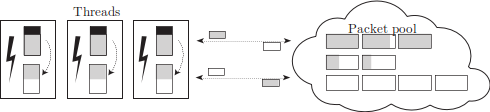
\includegraphics{figures/par_2}
  \caption[Γκρι πακέτα.]
    {Γκρι πακέτα. Κάθε νήμα ανταλλάσσει ένα άδειο πακέτο με
     ένα πακέτο αναφορών προς αντικείμενα προς εξιχνίαση. Η
     σήμανση γεμίζει ένα άδειο πακέτο με νέες αναφορές προς
     αντικείμενα προς εξιχνίαση: όταν αυτό γεμίσει, το νήμα
     το ανταλλάσσει με ένα καινούριο άδειο πακέτο από την
     καθολική δεξαμενή.}
  \label{fig:par_2}
\end{figure}

\subsection{Γκρι πακέτα}
Ο Ossia κ.ά \cite{DBLP:conf/pldi/OssiaBGKLO02}, καθώς και ο
Barabash κ.ά \cite{DBLP:journals/toplas/BarabashBGKLOOP05} 
παρατηρούν πώς η χρήση στοιβών
σήμανσης και κλοπής εργασίας είναι βέλτιστη όταν ο αριθμός των
νημάτων που συμμετέχουν στη συλλογή είναι γνωστός εξαρχής. Αυτό
δε συμβαίνει εάν κάθε νήμα τροποποιητής συμμετέχει πραγματοποιώντας
μια μικρή εργασία σε κάθε εκχώρηση. Επίσης παρατηρούν πώς είναι
πιθανόν δύσκολο για ένα νήμα να επιλέξει την καλύτερη ουρά από
την οποία θα κλέψει και ταυτόχρονα να εντοπίσει τον τερματισμό
της σήμανσης. Αντ'αυτού, εξισορροπούν το υπολογιστικό φορτίο
βάζοντας κάθε νήμα σήμανσης να ανταγωνίζεται για την απόκτηση
\textbf{πακέτων} αποτελούμενων από εργασίες σήμανσης. Το σύστημα
τους χρησιμοποιεί ένα σταθερό αριθμό από 1000 πακέτα των 512
εγγραφών το καθένα.

Κάθε νήμα σήμανσης χρησιμοποιεί δύο πακέτα: επεξεργάζεται
καταχωρίσεις από το πακέτο εισόδου και προσθέτει εργασίες 
σήμανσης στο πακέτο εξόδου. Ο όρος \textbf{γκρι πακέτα} οφείλεται 
στο γεγονός ότι τόσο το πακέτο εισόδου όσο και το πακέτο εξόδου
περιλαμβάνουν γκρι εγγραφές (αναφορές προς γκρι αντικείμενα)
σύμφωνα με την τριχρωματική αφαίρεση. Κάθε νήμα σήμανσης ανταγωνίζεται
με στόχο να αποκτήσει ένα πακέτο από μια καθολική δεξαμενή.
Αφού επεξεργασθεί όλες τις καταχωρίσεις ενός πακέτου, το επιστρέφει
στη δεξαμενή. Όταν το πακέτο εξόδου του είναι πλήρες, το επιστρέφει
στη δεξαμενή και παίρνει πίσω ένα φρέσκο πακέτο. Όπως φαίνεται
και στο σχήμα~\ref{fig:par2}, η κεντρική δεξαμενή αποτελείται
από τρεις συνδεδεμένες λίστες εκ των οποίων η πρώτη αποτελείται
από τελείως άδεια πακέτα, η δεύτερη από πακέτα σχεδόν μισογεμάτα
και η τρίτη από πακέτα σχεδόν γεμάτα. Τα νήματα προτιμούν την
τρίτη για την εισαγωγή ενός πακέτου εισόδου (\textproc{getInPacket})
και την πρώτη για την εξαγωγή ενός πακέτου εξόδου (\textproc{getOutPacket}).

Η τεχνική της παραλληλοποίησης της σήμανσης με γκρι πακέτα έχει
διάφορα πλεονεκτήματα. Ξεχωρίζοντας την είσοδο από την έξοδο,
ο Ossia κ.ά αποφεύγουν την εναλλαγή των ρόλων για τα πακέτα
ενός νήματος σήμανσης: το φορτίο εργασίας κατανέμεται ομοιόμορφα
στους επεξεργαστές καθώς ένας επεξεργαστής έχει την τάση να μην
καταναλώνει την έξοδό του. Καθώς ένα γκρι πακέτο περιλαμβάνει
μια ουρά από (αναφορές σε) αντικείμενα που θα επεξεργασθούν με
τη σειρά, προσφέρεται η δυνατότητα προφόρτωσης των επόμενων
αντικειμένων προς σήμανση.

Η τεχνική απαιτεί συγχρονισμό μόνο κατά τη μεταφορά των πακέτων
από και προς την καθολική δεξαμενή. Αυτό μειώνει τον αριθμό
των εντολών μνήμης \textbf{fence} που πρέπει να εισαχθούν από
το μεταγλωττιστή σε αρχιτεκτονικές με χαλαρό μοντέλο συνέπειας
μνήμης. Ένα νήμα χρειάζεται να εκτελέσει μία εντολή \textbf{fence}
μόνο όταν αποκτά πακέτα από την καθολική δεξαμενή ή επιστρέφει
πακέτα προς αυτή, και όχι μετά τη σήμανση και ώθηση ενός αντικειμένου
σε ένα πακέτο. Ο Ossia κ.ά χρησιμοποιούν ένα δίανυσμα από
\textbf{bits σήμανσης} όταν σαρώνουν συντηρητικά τις στοίβες
των νημάτων τροποποιητών προκειμένου να προσδιορίσουν αν μία
υποτιθέμενη αναφορά πραγματικά δείχνει προς κάποιο εκχωρηθέν
αντικείμενο. Τα bits σήμανσης χρησιμοποιούνται επίσης για το
συγχρονισμό μεταξύ των νημάτων τροποποιητών και των νημάτων
συλλεκτών. Οι εκχωρητές μνήμης χρησιμοποιούν τοπικούς απομονωτές
εκχώρησης. Κατά την υπερχείλιση ενός τοπικού απομονωτή εκχώρησης,
ο εκχωρητής εκτελεί μία εντολή \textbf{fence} και στη συνέχεια
θέτει σε λογικό 1 τα bits όλων των αντικείμενων που έχουν
εκχωρηθεί στον τοπικό απομονωτή, εξασφαλίζοντας με τον τρόπο
αυτό πώς οι αποθηκεύσεις που αφορούν την εκχώρηση και αρχικοποίηση
νέων αντικειμένων δεν προηγούνται των αποθηκεύσεων που αφορούν
την ενημέρωση των bits σήμανσης τους. Δύο ακόμη εντολές \textbf{fence}
είναι απαραίτητες. Πρώτον, όταν ένα νήμα εξιχνίασης αποκτά ένα
καινούριο πακέτο εισόδου, ελέγχει τα bits εκχώρησης όλων των
αντικειμένων του πακέτου και καταγράφει σε μία ιδιωτική δομή
δεδομένων για κάθε τέτοιο αντικείμενο αν είναι ασφαλής η
εξιχνίαση με ρίζα αυτό (αν το αντίστοιχο bit είναι σε λογικό
1). Στη συνέχεια το νήμα εκτελεί μία εντολή \textbf{fence}
πριν προχωρήσει στην εξιχνίαση με ρίζες τα ασφαλή αντικείμενα. 
Η εξιχνίαση με ρίζες τα μη ασφαλή αντικείμενα αναβάλλεται:
αυτά προστίθενται σε ένα πακέτο αναβολής, το οποίο κάποια
στιγμή αργότερα θα μεταφερθεί σε μία καθολική δεξαμενή
πακέτων αναβολής. Δεύτερον, ένα νήμα εξιχνίασης εκτελεί
μια εντολή \textbf{fence} όταν επιστρέφει το πακέτο εξόδου
του στην καθολική δεξαμενή (για να αποτρέψει την αναδιάταξη
αποθηκεύσεων στο πακέτο με την προσθήκη του πακέτου στην
καθολική δεξαμενή). Κατά την απόκτηση ενός πακέτου εισόδου
από την καθολική δεξαμενή υπάρχει μια εξάρτηση δεδομένων
μεταξύ της φόρτωσης του δείκτη προς το πακέτο και την πρόσβαση
στα περιεχόμενα και οι σύγχρονες αρχιτεκτονικές δεν αναδιατάσσουν
τις παραπάνω ενέργειες. Συνεπώς η εκτέλεση μιας εντολής
\textbf{fence} δεν είναι απαραίτητη σε αυτήν την περίπτωση.

Η τεχνική των γκρι πακέτων καθιστά εξαιρετικά απλή την
παρακολούθηση της κατάστασης. Κάθε καθολική δεξαμενή συσχετίζεται
με έναν καθολικό μετρητή του πλήθους των πακέτων της. Ο μετρητής
ενημερώνεται ατομικά κατά την προσθήκη ή αφαίρεση ενός
πακέτου από τη δεξαμενή. Η μέτρηση του πλήθους των πακέτων
είναι προσεγγιστική καθώς η μέτρηση μπορεί να διαβασθεί
αμέσως μετά την προσθήκη ενός πακέτου αλλά πριν την αύξηση
του μετρητή. Ωστόσο η συνθήκη τερματισμού απλώς ορίζει
ο μετρητής της καθολικής δεξαμενής άδειων πακέτων να ισούται
με το πλήθος των διαθέσιμων πακέτων. Η απόκτηση/επιστροφή
ενός πακέτου και η ενημέρωση του μετρητή της αντίστοιχης
καθολικής δεξαμενής δε χρειάζεται να είναι μία ενιαία
αδιαίρετη λειτουργία. Για να εξασφαλισθεί πώς ο μετρητής
κενών πακέτων δε θα μηδενισθεί προσωρινά, κάθε νήμα πρέπει
να αποκτήσει ένα καινούριο πακέτο εισόδου πριν επιστρέψει
το πακέτο εξόδου του στην καθολική δεξαμενή. 

\begin{algorithm}[H]
  \caption{Διαχείριση γκρι πακέτων}
  \label{alg:par4}
  \begin{algorithmic}[1]
    \State \textbf{shared} $fullPool$ \Comment{global pool of full packets}
    \State \textbf{shared} $halfFullPool$ \Comment{global pool of half full packets}
    \State \textbf{shared} $emptyPool$ \Comment{global pool of empty packets}
    \Statex
    \Function{getInPacket}{\null}
      \State \textbf{atomic}
      \State $inPacket \gets$ \Call{remove}{$fullPool$}
      \If{\Call{isEmpty}{$inPacket$}}
        \State \textbf{atomic}
        \State $inPacket \gets$ \Call{remove}{$halfFullPool$}
      \EndIf
      \If{\Call{isEmpty}{$inPacket$}}    
        \State $inPacket, outPacket \gets outPacket, inPacket$
      \EndIf
      \State \Return{\textbf{not} \Call{isEmpty}{$inPacket$}}
    \EndFunction
    \Statex
    \Procedure{testAndMarkSafe}{$packet$}
      \ForAll{$ref \; \textbf{in} \; packet$}
        \State \Call{safe}{$ref$} $\gets$ \Call{allocBit}{$ref$} $=\textbf{true}$ \Comment{private data structure}
      \EndFor
    \EndProcedure
    \Statex
    \Procedure{getOutPacket}{\null}
      \If{\Call{isFull}{$outPacket$}}
        \State \Call{generateWork}{\null}
      \EndIf
      \If{$outPacket = \textbf{null}$}
        \State \textbf{atomic}
        \State $outPacket \gets$ \Call{remove}{$emptyPool$}
      \EndIf
      \If{$outPacket = \textbf{null}$}
        \State \textbf{atomic}
        \State \Call{remove}{$halfFullPool$}
      \EndIf
      \If{$outPacket = \textbf{null}$}
        \If{\textbf{not} \Call{isFull}{$inPacket$}}    
          \State $inPacket, outPacket \gets outPacket, inPacket$
          \State \Return{\null}
        \EndIf  
      \EndIf
    \EndProcedure
    \Statex
    \Procedure{addOutPacket}{$ref$}
      \State \Call{getOutPacket}{\null}
      \If{$outPacket = \textbf{null}$ \textbf{or} \Call{isFull}{$outPacket$}}
        \State \Call{dirtyCard}{$ref$}
      \Else
        \State \Call{add}{$outPacket$, $ref$}
      \EndIf
    \EndProcedure
  \end{algorithmic}
\end{algorithm}

\begin{algorithm}[H]
  \caption{Παράλληλη εκχώρηση με χρήση γκρι πακέτων}
  \label{alg:par5}
  \begin{algorithmic}[1]
    \Function{sequentialAllocate}{$n$}
      \State $result \gets free$
      \State $newFree \gets result + n$
      \If{$newFree \leq labLimit$}
        \State $free \gets newFree$
        \State \Return{$result$}
      \EndIf
      \Statex
      \State /* local allocation buffer overflow */
      \State \textbf{fence}
      \ForAll{$obj \; \textbf{in} \; lab$}
        \State \Call{allocBit}{$obj$} $\gets \textbf{true}$
      \EndFor
      \State $lab, labLimit \gets$ \Call{newLab}{\null}
      \If{$lab = \textbf{null}$}
        \State \Return{\textbf{null}}
      \EndIf
      \State \Call{sequentialAllocate}{$n$} \Comment{signal 'Memory exhausted'}
    \EndFunction
  \end{algorithmic}
\end{algorithm}

\begin{algorithm}[H]
  \caption{Παράλληλη σήμανση με χρήση γκρι πακέτων}
  \label{alg:par6}
  \begin{algorithmic}[1]
    \State \textbf{shared} $fullPool$ \Comment{global pool of full packets}
    \Statex
    \Procedure{acquireWork}{\null}
      \If{\Call{isEmpty}{$inPacket$}}
        \If{\Call{getInPacket}{\null}}
          \State \Call{testAndMarkSafe}{$inPacket$}
          \State \textbf{fence}
        \EndIf
      \EndIf
    \EndProcedure
    \Statex
    \Procedure{performWork}{\null}
      \ForAll{$ref \; \textbf{in} \; inPacket$}
        \If{\Call{safe}{$ref$}}
          \ForAll{$fld \; \textbf{in} \; Pointers(ref)$}
            \State $child \gets *fld$
            \If{$child \neq \textbf{null}$ \textbf{and} \textbf{not} \Call{isMarked}{$child$}}
              \State \Call{setMarked}{$child$}
              \State \Call{addOutPacket}{$child$}
            \EndIf
          \EndFor   
        \Else
          \State \Call{addDeferredPacket}{$ref$} \Comment{defer tracing of unsafe objects}
        \EndIf
      \EndFor
    \EndProcedure
    \Statex
    \Procedure{generateWork}{\null}
      \State \textbf{fence}
      \State \Call{add}{$fullPool$, $outPacket$}
      \State $outPacket \gets \textbf{null}$
    \EndProcedure
  \end{algorithmic}
\end{algorithm}

\section{Παράλληλη αντιγραφή}
Η παραλληλοποίηση των αλγορίθμων συλλογής με αντιγραφή αντιμετωπίζει
λίγο πολύ τα ίδια ζητήματα με την παραλληλοποίηση των αλγορίθμων
συλλογής με σήμανση. Ωστόσο, παρότι η σήμανση ενός αντικειμένου
δύο φορές είναι αβλαβής, αυτό πρέπει να αντιγραφεί μόνο μία φορά.

\subsection{Διαμοιρασμός εργασίας ανάμεσα στους επεξεργαστές}
Οι Blelloch και Cheng \cite{DBLP:conf/pldi/BlellochC99, DBLP:conf/pldi/ChengB01}
παραλληλοποιούν την αντιγραφή στα πλαίσια της \textbf{επαναληπτικής
συλλογής}.

Οι επαναληπτικοί συλλέκτες είναι αυξητικοί ή ταυτόχρονοι συλλέκτες
που αντιγράφουν αντικείμενα την ώρα εκτέλεσης του τροποποιητή,
λαμβάνοντας ειδική φροντίδα για την επιδιόρθωση πεδίων που
εγγράφησαν από τον τροποποιητή κατά τη διάρκεια ενός κύκλου
συλλογής.

Κάθε νήμα αντιγραφής έχει τη δική του στοίβα εργασίας. Οι Blelloch
και Cheng ισχυρίζονται πώς οι στοίβες προσφέρουν ευκολότερο
συγχρονισμό μεταξύ των νημάτων αντιγραφής όπως επίσης και μικρότερο
ποσοστό κατακερματισμού από ότι οι ουρές Cheney. Το φορτίο εργασίας
εξισορροπείται βάζοντας τα νήματα αντιγραφής να μεταφέρουν περιοδικά
μονάδες εργασίας μεταξύ των τοπικών στοιβών και μιας καθολικής
στοίβας. Μια απλή μοιραζόμενη στοίβα απαιτεί το συγχρονισμό
μεταξύ των νημάτων που εκτελούν λειτουργίες ώθησης και εξώθησης
καταχωρίσεων. Δυστυχώς, δεν υπάρχει τρόπος ατομικής αύξησης
ή μείωσης του δείκτη στοίβας για την εισαγωγή και εξαγωγή ενός
στοιχείου με τη χρήση πρωταρχικών λειτουργιών όπως η \textproc{FetchAndAdd}
και η χρήση ενός κλειδώματος θα σειριοποιούσε την πρόσβαση στη
στοίβα. Η εντολή \textproc{FetchAndAdd} μπορεί ωστόσο να χρησιμοποιηθεί
ώστε να επιτραπεί σε πολλαπλά νήματα είτε να εισάγουν στοιχεία
στη στοίβα είτε να εξάγουν στοιχεία από τη στοίβα, καθώς
οι λειτουργίες αυτές έχουν ως τελικό αποτέλεσμα είτε την
αύξηση είτε τη μείωση του δείκτη στοίβας κατά περισσότερες
από μία θέσεις. Αφού ένα νήμα έχει πετύχει να μετακινήσει το
δείκτη στοίβας, πιθανώς κατά αρκετές θέσεις, μπορεί να διαβάσει
από η να γράψει στις θέσεις αυτές χωρίς τον κίνδυνο εμφάνισης
καταστάσεων συναγωνισμού.

Οι Cheng και Blelloch επιβάλλουν αυτού του είδους την πρόσβαση
στη μοιραζόμενη στοίβα χρησιμοποιώντας ένα μηχανισμό που
ονομάζουν \textbf{δωμάτια}. Υπάρχουν δύο δωμάτια: ένα ώθησης
και ένα εξώθησης και ανά πάσα χρονική στιγμή ένα εκ των δύο
πρέπει να είναι άδειο. Σε κάθε επανάληψη του βρόχου συλλογής,
ένα νήμα εισέρχεται αρχικά στο δωμάτιο εξώθησης και εκτελεί
ένα προκαθορισμένο αριθμό μονάδων εργασίας. Αποκτά αντικείμενα προς
σάρωση είτε από την τοπική του στοίβα είτε από την καθολική
στοίβα με χρήση της εντολής \textproc{FetchAndAdd}. Οι παραγόμενες
μονάδες εργασίας εισάγονται στην τοπική στοίβα. Στη συνέχεια
το νήμα εγκαταλείπει το δωμάτιο εξώθησης και περιμένει μέχρις
ότου και τα υπόλοιπα νήματα το έχουν εγκαταλείψει πριν προσπαθήσει
να εισέλθει στο δωμάτιο ώθησης. Το πρώτο νήμα που καταφέρνει
να εισέλθει κλείνει την πόρτα (μεταβλητή $gate$) ούτως ώστε
να απαγορευθεί η είσοδος στα υπόλοιπα νήματα. Ενώ βρίσκεται
μέσα στο δωμάτιο ώθησης, το νήμα αδειάζει πλήρως την τοπική
του στοίβα, μεταφέροντας όλα τα στοιχεία της στην καθολική
στοίβα, αφού πρώτα δεσμεύσει τον απαραίτητο χώρο με την εντολή
\textproc{FetchAndAdd}. Το τελευταίο νήμα που αποχωρεί από
το δωμάτιο ώθησης κλείνει την πύλη.

Το πρόβλημα του μηχανισμού είναι πώς ένας επεξεργαστής που
περιμένει για να εισέλθει στο δωμάτιο ώθησης υποχρεούται
να περιμένει μέχρις ότου όλοι οι επεξεργαστές που βρίσκονται
ήδη μέσα τελειώσουν τη σήμανση των αντικειμένων τους με
γκρι χρώμα. Ο χρόνος σήμανσης των αντικειμένων με γκρι
χρώμα είναι συγκρίσιμος με το χρόνο απόκτησης ή κατάθεσης
νέων μονάδων εργασίας και ένας επεξεργαστής που προσπαθεί
να εισέλθει στη φάση ώθησης πρέπει να περιμένει μέχρις ότου
όλοι οι υπόλοιποι επεξεργαστές που βρίσκονται στη φάση
εξώθησης τελειώσουν τη σήμανση των αντικειμένων τους με
γκρι χρώμα. Μεγάλες διακυμάνσεις στο χρόνο που χρειάζονται
οι επεξεργαστές για τη σήμανση των αντικειμένων τους με γκρι
χρώμα καθιστούν αυτό το χρόνο αδράνειας σημαντικό. Μια πιο
χαλαρή αφαίρεση θα επέτρεπε στους επεξεργαστές να εγκαταλείψουν
το δωμάτιο εξώθησης χωρίς να εισέλθουν στο δωμάτιο ώθησης.
Καθώς η σήμανση των αντικειμένων με γκρι χρώμα δε σχετίζεται
με τη μοιραζόμενη στοίβα, αυτή η εργασία μπορεί να πραγματοποιηθεί
εκτός των δωματίων. Αυτό αυξάνει σημαντικά την πιθανότητα
το δωμάτιο εξώθησης να είναι άδειο και συνεπώς ένα νήμα να
μπορέσει να εισέλθει στο δωμάτιο ώθησης.

Ο αρχικός μηχανισμός δωματίων των Cheng και Blelloch επιτρέπει
απλή ανίχνευση τερματισμού. Η τοπική στοίβα κάθε νήματος
είναι κενή όταν αυτό εγκαταλείπει το δωμάτιο ώθησης και επομένως
μένει στο τελευταίο νήμα που αποχωρεί να ελέγξει αν και
η καθολική μοιραζόμενη στοίβα είναι επίσης άδεια. Ωστόσο,
ο χαλαρός ορισμός του μηχανισμού των δωματίων επιτρέπει
στα νήματα να εργάζονται και εκτός δωματίων. Η υιοθέτηση αυτού
συνεπάγεται πώς η μοιραζόμενη στοίβα πρέπει να διατηρεί μία
καθολική μεταβλητή που μετράει πόσα νήματα έχουν δανεισθεί
αντικείμενα από αυτή. Το τελευταίο νήμα που αποχωρεί από το
δωμάτιο ώθησης ελέγχει ταυτόχρονα αν η μοιραζόμενη στοίβα είναι
κενή και ο καθολικός αυτός μετρητής μηδενικός.

\begin{algorithm}[H]
  \caption{Παράλληλη αντιγραφή (Cheng \& Blelloch)}
  \label{alg:par_7}
  \begin{algorithmic}[1]
    \State \textbf{shared} sharedStack \Comment{the shared stack of work}
    \State $myCopyStack[k]$ \Comment{local stack has k slots max}
    \State $sp \gets 0$
    \Statex
    \Procedure{run}{\null}
      \While{\textbf{not} \Call{terminated}{\null}}
        \State \Call{enterRoom}{\null} \Comment{enter pop room}
        \For{$i \gets 1 \; \textbf{to} \; k$}
          \If{\Call{isLocalStackEmpty}{\null}}
            \State \Call{acquireWork}{\null}
            \If{\Call{isLocalStackEmpty}{\null}}
              \State \textbf{break} 
            \EndIf
          \EndIf
          \State \Call{performWork}{\null}
        \EndFor
        \State \Call{generateWork}{\null}
        \If{\Call{exitRoom}{\null}} \Comment{leave push room}
          \State \Call{terminate}{\null}
        \EndIf
     \EndWhile
   \EndProcedure
   \Statex
   \Procedure{acquireWork}{\null} \Comment{move work from shared stack}
     \State \Call{sharedPop}{\null}
   \EndProcedure
   \Statex
   \Procedure{performWork}{\null}
     \State $ref \gets$ \Call{localPop}{\null}
     \State \Call{scan}{$ref$} \Comment{see algorithm~\ref{alg:cop_2}}
   \EndProcedure
   \Statex
   \Procedure{generateWork}{\null} \Comment{move work to shared stack}
     \State \Call{sharedPush}{\null}
   \EndProcedure
   \Statex
   \Function{isLocalStackEmpty}{\null}
     \State \Return{$sp=0$}
   \EndFunction
   \Statex
   \Procedure{localPush}{$ref$}
     \State $myCopyStack[sp++] \gets ref$
   \EndProcedure
   \Statex
   \Function{localPop}{\null}
     \Return{$myCopyStack[--sp]$}
   \EndFunction
   \Statex
   \Procedure{sharedPop}{\null} \Comment{move work from shared stack}
     \State $cursor \gets$ \Call{FetchAndAdd}{$\&sharedStack$, $1$} \Comment{try to grab from shared stack} 
     \If{$cursor > stackLimit$} \Comment{shared stack empty}
       \State \Call{FetchAndAdd}{$\&sharedStack$, $-1$} \Comment{readjust stack}
     \Else
       \State $myCopyStack[sp++] \gets cursor[0]$ \Comment{move work to local stack}
     \EndIf
   \EndProcedure
   \Statex
   \Procedure{sharedPush}{\null} \Comment{move work to shared stack}
     \State $cursor \gets$ \Call{FetchAndAdd}{$\&sharedStack$, $-sp$} $-sp$
     \For{$i \gets 0 \; \textbf{to} \; sp-1$}
       \State $cursor[i] \gets myCopyStack[i]$
     \EndFor
     \State $sp \gets 0$
   \EndProcedure
  \end{algorithmic}
\end{algorithm}

\begin{algorithm}[H]
  \caption{Συγχρονισμός λειτουργιών ώθησης/εξώθησης με δωμάτια}
  \label{alg:par_8}
  \begin{algorithmic}[1]
    \State \textbf{shared} $gate \gets OPEN$
    \State \textbf{shared} $popClients$ \Comment{number of clients currently in the pop room}
    \State \textbf{shared} $pushClients$ \Comment{number of clients currently in the push room}
    \Statex
    \Procedure{enterRoom}{\null}
      \While{$gate \neq OPEN$} \Comment{do nothing:wait}
      \EndWhile
      \State \Call{FetchAndAdd}{$\&popClients$, $1$} \Comment{try to start popping}
      \While{$gate \neq OPEN$}
        \State \Call{FetchAndAdd}{$\&popClients$, $-1$} \Comment{back out since did not succeed}
         \While{$gate \neq OPEN$} \Comment{do nothing:wait}
         \EndWhile
         \State \Call{FetchAndAdd}{$\&popClients$, $1$} \Comment{try again}
      \EndWhile
    \EndProcedure
    \Statex
    \Procedure{transitionRooms}{\null}
      \State $gate \gets CLOSED$
      \State \Call{FetchAndAdd}{$\&pushClients$, $1$} \Comment{move from popping to pushing}
      \State \Call{FetchAndAdd}{$\&popClients$, $-1$}
      \While{$popClients > 0$} \Comment{can't start pushing until none other popping}
      \EndWhile
    \EndProcedure
    \Statex
    \Procedure{exitRoom}{\null}
      \State $pushers \gets$ \Call{FetchAndAdd}{$\&pushClients$, $-1$} $-1$ \Comment{stop pushing}
      \If{$pushers = 0$} \Comment{I was last in room: check termination}
        \If{\Call{isEmpty}{$sharedStack$}}
          \State $gate \gets OPEN$
          \State \Return{\textbf{true}}
        \Else
          \State $gate \gets OPEN$
          \State \Return{\textbf{false}}
        \EndIf
      \EndIf
    \EndProcedure
  \end{algorithmic}
\end{algorithm}

\subsection{Αντιγράφοντας αντικείμενα παράλληλα}
Για να εξασφαλισθεί πώς μόνο ένα νήμα αντιγράφει ένα αντικείμενο,
τα νήματα πρέπει να συναγωνισθούν ώστε να αντιγράψουν ένα αντικείμενο
και να εγκαταστήσουν τη διεύθυνση προώθησης στην επικεφαλίδα
του παλαιού του αντιγράφου. Ο τρόπος αντιγραφής ενός αντικειμένου
από τα νήματα εξαρτάται από το εάν αυτά μοιράζονται μια μοναδική
περιοχή εκχώρησης μνήμης. Στην περίπτωση αυτή, τα νήματα αποφεύγουν
ορισμένη σπατάλη πληρώνοντας όμως το κόστος της χρήσης μιας
ατομικής λειτουργίας για εκχώρηση. Σε αυτήν την περίπτωση, οι
Blelloch και Cheng \cite{DBLP:conf/pldi/BlellochC99} θέτουν
να νήματα σε ανταγωνισμό για την εγγραφή μιας ειδικής τιμής
'busy' στην λέξη της επικεφαλίδας του αντικειμένου όπου θα
αποθηκευθεί η διεύθυνση προώθησης αυτού. Το νήμα νικητής αντιγράφει
το αντικείμενο πριν αποθηκεύσει τη διεύθυνση προώθησης, ενώ
τα νήματα ηττημένοι πρέπει να σπινάρουν μέχρις ότου παρατηρήσουν
μία έγκυρη διεύθυνση. Εναλλακτικά, αν κάθε νήμα γνωρίζει εξαρχής
σε ποια θέση θα αντιγράψει ένα αντικείμενο (για παράδειγμα
επειδή θα το αντιγράψει σε έναν τοπικό απομονωτή εκχώηρησης),
είναι τα νήματα να ανταγωνίζονται για να εγγράψουν ατομικά
τη διεύθυνση προώθησης προτού αντιγράψουν το αντικείμενο.

Ο συλλέκτης της Flood κ.ά \cite{DBLP:conf/jvm/FloodDSZ01} στον
οποίο αναφερθήκαμε προηγουμένως είναι γενεαλογικός. Η παλαιά
γενεά διαχειρίζεται από συλλογή με σήμανση και συμπύκνωση και
η νέα γενεά από συλλογή με αντιγραφή. Είδαμε παραπάνω τον
τρόπο με τον οποίο παραλληλοποιούν τη φάση της σήμανσης.
Εξετάζουμε τώρα πώς παραλληλοποιούν την αντιγραφή. Διπλά-τερματισμένες
κλεπτόμενες ουρές χρησιμοποιούνται και εδώ για τη διαχείριση
των αντικειμένων που πρόκειται να σαρωθούν. Ωστόσο, η παράλληλη αντιγραφή αντιμετωπίζει δύο
προβλήματα άγνωστα στην παράλληλη σήμανση: πρώτον, είναι επιθυμητή
η ελαχιστοποίηση του ανταγωνισμού για την εκχώρηση μνήμης όπου
θα αντιγραφεί ένα αντικείμενο και δεύτερον ένα ζωντανό αντικείμενο
πρέπει να αντιγραφεί μόνο μία φορά. Ο ανταγωνισμός για την
εκχώρηση μνήμης ελαχιστοποιείται με τη χρήση τοπικών απομονωτών
εκχώρησης για κάθε νήμα, τόσο για την αντιγραφή στους χώρους
επιζώντων στη νέα γενεά όσο και για την προαγωγή στην παλαιά
γενεά. Για να αντιγράψει ένα αντικείμενο, ένα νήμα πραγματοποιεί
μια υποθετική εκχώρηση στον τοπικό του απομονωτή εκχώρησης
και στη συνέχεια επιχειρεί μια πράξη \textproc{CompareAndSwap}
στον δείκτη προώθησης. Αν η τελευταία πετύχει, το νήμα αντιγράφει
το αντικείμενο. Αν όχι, επιστρέφει την τιμή του δείκτη προώθησης
που εγκατέστησε το νήμα νικητής.

\begin{figure}[H]
  \centering
  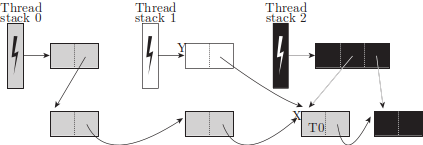
\includegraphics{figures/par_3}
  \caption[Εξιχνίαση κυρίαρχου νήματος.]
    {Εξιχνίαση κυρίαρχου νήματος. Τα νήματα 0 έως 2 με χρώμα
     μαύρο γκρι και άσπρο αντίστοιχα, έχουν εξιχνιάσει ένα
     γράφο αντικειμένων. Το χρώμα κάθε αντικειμένου υποδεικνύει
     τον επεξεργαστή στη μνήμη του οποίου θα αντιγραφεί. Το
     πρώτο πεδίο κάθε αντικειμένου είναι η επικεφαλίδα του.
     Το νήμα $T0$ είναι αυτό που τελευταίο κλείδωσε το αντικείμενο
     $X$.}
  \label{fig:par_3}
\end{figure}

 Ο διαχειριστής μνήμης του Ogasawara \cite{DBLP:conf/oopsla/Ogasawara09}
 λαμβάνει υπόψη την μη ομοιόμορφη προσπέλαση μνήμης και
 διαιρεί το σωρό σε τμήματα με μία ή περισσότερες σελίδες
 και κάθε τμήμα απεικονίζεται με έναν επεξεργαστή. Ο εκχωρητής
 μνήμης, ο οποίος χρησιμοποιείται τόσο από τα νήματα τροποποιητές
 όσο και από τα νήματα συλλέκτες προτιμά να εκχωρεί μπλοκ από
 τη μνήμη του προτιμώμενου επεξεργαστή. Για ένα νήμα τροποποιητή,
 αυτός ταυτίζεται με τον επεξεργαστή στον οποίο εκτελείται το
 νήμα. Τα νήματα συλλέκτες προσπαθούν πάντοτε να αντιγράψουν
 ζωντανά αντικείμενα σε σελίδες μνήμης που σχετίζονται με τον
 προτιμώμενο επεξεργαστή των τελευταίων. Καθώς το νήμα στο
 οποίο εκχωρήθηκε ένα αντικείμενο δεν είναι απαραίτητα και το
 νήμα που το χρησιμοποιεί περισσότερο συχνά, ο συλλέκτης
 χρησιμοποιεί πληροφορία \textbf{κυρίαρχου νήματος} για να
 προσδιορίζει τον προτιμώμενο επεξεργαστή κάθε αντικειμένου.
 Πρώτον, ο προτιμώμενος επεξεργαστής αντικειμένων προς τα οποία
 υπάρχουν άμεσες αναφορές από τη στοίβα ενός νήματος τροποποιητή
 θα είναι ο επεξεργαστής στον οποίο το νήμα εκτελέσθηκε για
 τελευταία φορά. Αυτό πιθανόν να δημιουργεί την απαίτηση τα
 νήματα να ενημερώνουν περιοδικά την ταυτότητα του προτιμώμενου
 επεξεργαστή τους. Δεύτερον, ο συλλέκτης μπορεί να χρησιμοποιήσει
 πληροφορίες σχετικές με το κλείδωμα αντικειμένων για να ταυτοποιήσει
 το \textbf{κυρίαρχο νήμα}. Οι μηχανισμοί κλειδωμάτων συχνά
 αποθηκεύουν την ταυτότητα του νήματος που έχει κλειδώσει ένα
 αντικείμενο σε μια λέξη στην επικεφαλίδα του αντικειμένου.
 Παρότι με αυτόν τον τρόπο ταυτοποιείται το νήμα (και συνεπώς
 και ο αντίστοιχος επεξεργαστής) που τελευταίο κλείδωσε το
 αντικείμενο, η προσέγγιση αυτή φαντάζει αρκετή καθώς τα
 περισσότερα αντικείμενα δεν ξεφεύγουν ποτέ από το νήμα στο
 οποίο εκχωρήθηκαν. Τέλος, ο συλλέκτης μπορεί να διαδώσει
 την ταυτότητα του προτιμώμενου επεξεργαστή από αντικείμενα
 γονείς σε αντικείμενα παιδιά.
  
 \subsection{Ξεχωριστοί ημιχώροι-από και ημιχώροι-προς}
 Η συλλογή με αντιγραφή από τη φύση
 \subsection{Σωροί οργανωμένοι κατά μπλοκ}
 Μία προσέγγιση είναι να υπερ-διαμερισθεί ο χώρος-προς και στη
 συνέχεια να νήματα να τεθούν σε ανταγωνισμό για την απόκτηση
 μπλοκ σάρωσης και αντιγραφής. Ο Imai κ.ά \cite{DBLP:journals/tpds/ImaiT93}
 διαιρούν το σωρό σε \textbf{κομμάτια (chunks)} σταθερού μεγέθους
 και παρέχουν σε κάθε νήμα τα δικά του κομμάτια σάρωσης
 και αντιγραφής επιζώντων αντικειμένων. Όταν το κομμάτι αντιγραφής
 ενός νήματος γεμίσει, αυτό μεταφέρεται σε μια καθολική δεξαμενή
 και τα ανενεργά νήματα ανταγωνίζονται για την απόκτηση και
 σάρωση του και το αρχικό νήμα αποκτά ένα καινούριο κομμάτι
 από το διαχειριστή ελεύθερων κομματιών.

 Δύο μηχανισμοί χρησιμοποιούνται για την εξισορρόπηση του φορτίου
 εργασίας. Αρχικά, τα κομμάτια αντιγραφής (τα οποία ονομάζουν
 μονάδες επέκτασης σωρού) είναι σχετικά μικρά (256 λέξεις). Δεύτερον,
 κάθε κομμάτι διαιρείται σε μικρότερα \textbf{μπλοκ} (τα οποία
 ονομάζουν μονάδες κατανομής φορτίου), με τυπικό μέγεθος 32 λέξεις.
 Κάθε νήμα προσφέρεται να παραχωρήσει μερικά από τα μη σαρωμένα
 μπλοκ του οποτεδήποτε χρειάζεται ένα νέο μπλοκ σάρωσης.  
 
 \section{Παράλληλη εκκαθάριση}
 Eξετάζουμε τώρα πώς μπορούν να παραλληλοποιηθούν οι φάσεις
 της εκκαθάρισης και της συμπύκνωσης. Και οι δύο φάσεις έχουν την
 ιδιότητα πώς η εξιχνίαση έχει ολοκληρωθεί και τα ζωντανά αντικείμενα
 του σωρού εντοπισθεί. Επίσης και οι δύο είναι εγγενώς παραλληλοποιήσιμες.

 Η παραλληλοποίηση της εκκαθάρισης μπορεί να επιτευχθεί είτε διαμερίζοντας
 στατικά το σωρό σε συνεχόμενες περιοχές, είτε υπερ-διαμερίζοντας
 τον σε μπλοκ και αφήνοντας να νήματα να ανταγωνίζονται για την
 εκκαθάριση ενός μπλοκ σε μία καθολική ελεύθερη λίστα μπλοκ. Ωστόσο,
 με την υιοθέτηση αυτής της απλής στρατηγικής είναι πιθανόν η ελεύθερη
 λίστα να καταστεί σημείο συμφόρησης και η συλλογή να σειριοποιηθεί.
 Ευτυχώς όμως σε ένα τέτοιου είδους παράλληλο σύστημα, κάθε επεξεργαστής
 διατηρεί συνήθως τοπικές ξεχωριστές ελεύθερες λίστες με μπλοκ
 διαφορετικών μεγεθών για την εκχώρηση μνήμης και έτσι το πρόβλημα
 του ανταγωνισμού ανάγεται στο χειρισμό της επιστροφής ολόκληρων
 ελεύθερων μπλοκ σε έναν καθολικό εκχωρητή μπλοκ. Επιπλέον, η
 οκνηρή εκκαθάριση αποτελεί από τη φύση της μιας παράλληλη λύση
 στο πρόβλημα της εκκαθάρισης μερικώς γεμάτων μπλοκ η οποία εξισορροπεί
 τις εργασίες εκκαθάρισης σύμφωνα με τους ρυθμούς εκχώρησης μνήμης
 στα νήματα τροποποιητές.

 Το πρώτο και μοναδικό βήμα της φάσης εκκαθάρισης όταν η τελευταία
 πραγματοποιείται οκνηρώς είναι η ταυτοποίηση πλήρως άδειων μπλοκ
 και η επιστροφή τους στον εκχωρητή μπλοκ. Για να μειώσουν τον
 ανταγωνισμό μεταξύ των νημάτων εκκαθάρισης, ο Endo κ.ά \cite{DBLP:conf/sc/EndoTY97}
 παρέχουν σε κάθε ένα από αυτά έναν αριθμό από συνεχόμενα μπλοκ
 προς τοπική επεξεργασία. Ο συλλέκτης τους χρησιμοποιεί bitmap
 σήμανσης, τα οποία αποθηκεύονται στις επικεφαλίδες των μπλοκ,
 ξεχωριστά από αυτά. Αυτή η προσέγγιση καθιστά εύκολο τον προσδιορισμό
 του κατά πόσο ένα μπλοκ είναι τελείως κενό από ζωντανά αντικείμενα.
 Τα άδεια μπλοκ ταξινομούνται και συνενώνονται πριν επιστραφούν
 σε μια τοπική ελεύθερη λίστα. Τα μερικώς γεμάτα από ζωντανά
 αντικείμενα μπλοκ εισάγονται σε τοπικές ξεχωριστές λίστες ανάκτησης
 για μπλοκ ξεχωριστών μεγεθών προς μελλοντική οκνηρή εκκαθάριση
 από τα νήματα τροποποιητές. Μόλις ένας επεξεργαστής ολοκληρώσει
 την εκκαθάριση του τοπικού του συνόλου εκκαθάρισης, συγχωνεύει
 την ελεύθερη λίστα μπλοκ αυτού με την καθολική ελεύθερη λίστα
 μπλοκ. Η τελευταία ερώτηση που μένει να απαντηθεί αφορά στο
 τι κάνει ένα νήμα τροποποιητής στην περίπτωση που τόσο η τοπική
 λίστα ανάκτησης όσο και η καθολική δεξαμενή μπλοκ είναι άδειες.
 Μια λύση είναι να κλέψει ένα μπλοκ από ένα άλλο νήμα, κάτι που
 απαιτεί το συγχρονισμό της απόκτησης του επόμενου μπλοκ προς
 εκκαθάριση. Το κόστος αυτό δεν είναι μεγάλο αν αναλογισθεί κανείς
 πώς αφενός η απόκτηση ενός μπλοκ προς εκκαθάριση συμβαίνει πιο
 σπάνια από ότι η αίτηση για εκχώρηση μνήμης στο εσωτερικό ενός
 μπλοκ και αφετέρου ο ανταγωνισμός πολλών νημάτων για την απόκτηση
 ενός μπλοκ προς εκκαθάριση δεν αναμένεται να συμβαίνει συχνά
 στην πράξη.

 \section{Παράλληλη συμπύκνωση}
 Η παραλληλοποίηση αλγορίθμων συλλογής σκουπιδιών με σήμανση
 και συμπύκνωση αφορά στην παράλληλη σήμανση των ζωντανών αντικειμένων
 και στη συνέχεια στην παράλληλη μετακίνηση αυτών. Ωστόσο η παράλληλη
 ολισθαίνουσα συμπύκνωση είναι απλούστερη από την παράλληλη
 αντιγραφή, τουλάχιστον σε συνεχόμενους σωρούς. Για παράδειγμα,
 όταν τα ζωντανά αντικείμενα έχουν σημανθεί ο προορισμός των αντικειμένων
 που θα μετακινηθούν δεν αλλάζει: οι καταστάσεις συναγωνισμού
 επηρεάζουν την επίδοση και όχι τόσο την ορθότητα. Μετά τη
 φάση της σήμανσης, οι περισσότεροι συλλέκτες με σήμανση και
 συμπύκνωση απαιτούν δύο ή και περισσότερα περάσματα στο σωρό
 προκειμένου να προσδιορίσουν τη διεύθυνση πρoώθησης κάθε αντικειμένου,
 να ενημερώσουν τις αναφορές προς κάθε αντικείμενο και να μετακινήσουν
 τα αντικείμενα. Όπως είδαμε στο κεφάλαιο \ref{ch:mark-compact}
 διαφορετικοί αλγόριθμοι μπορεί να εκτελούν αυτές τις εργασίες
 με διαφορετική σειρά ή να συνδυάσουν την εκτέλεση δύο εργασιών
 σε ένα μόνο πέρασμα.

 Ο Flood κ.ά \cite{DBLP:conf/jvm/FloodDSZ01} χρησιμοποιούν παράλληλη
 σήμανση και παράλληλη συμπύκνωση για τη διαχείριση της παλαιάς
 γενεάς στον παράλληλο γενεαλογικό συλλέκτη της εικονικής τους
 μηχανής για τη γλώσσα Java. Ο συλλέκτης χρησιμοποιεί τρεις επιπλέον
 φάσεις μετά την ολοκλήρωση της παράλληλης σήμανσης για να
 \begin{inparaenum}[(i)]
 \item υπολογίσει διευθύνσεις προώθησης
 \item ενημερώσει αναφορές και
 \item μετακινήσει αντικείμενα
 \end{inparaenum}. Το ενδιαφέρον χαρακτηριστικό της σχεδίασης
 τους είναι πώς χρησιμοποιούν διαφορετική στρατηγική εξισορρόπησης
 φορτίου σε κάθε διαφορετική φάση συμπύκνωσης. Οι αλγόριθμοι
 συμπύκνωσης για μονοεπεξεργαστικά συστήματα πραγματοποιούν την
 ολίσθηση των ζωντανών αντικειμένων στο ένα άκρο του σωρού.
 Αν όμως υπάρχουν πολλαπλά νήματα συμπύκνωσης μετακινούν αντικείμενα
 παράλληλα, τότε απαιτείται προσοχή ούτως ώστε να αποτραπεί η
 εγγραφή δεδομένων ενός ζωντανού αντικειμένου από ένα νήμα
 συμπύκνωσης πριν τη μετακίνησή του αντικειμένου από ένα άλλο
 νήμα συμπύκνωσης. Για το λόγο αυτό, ο Flood κ.ά δε συμπυκνώνουν
 όλα τα αντικείμενα σε ένα πυκνό άκρο του σωρού, αλλά αντίθετα
 διαιρούν το σωρό σε περιοχές και αναθέτουν σε κάθε νήμα συμπύκνωσης
 τη δική του περιοχή. Κάθε νήμα συμπύκνωσης είναι υπεύθυνο για
 την ολίσθηση ζωντανών αντικειμένων μόνο στη δική του περιοχή.
 Επιπλέον, προκειμένου να μειωθεί ο (περιορισμένος) κατακερματισμός
 που μπορεί να προκύψει από τη χρήση αυτής της στρατηγικής
 διαμέρισης του σωρού, η κατεύθυνση ολίσθησης αντικειμένων
 εναλλάσσεται μεταξύ δύο διαδοχικών περιοχών. 

\begin{figure}[H]
  \centering
  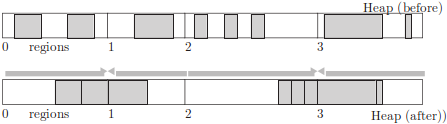
\includegraphics{figures/par_5}
  \caption
    [Διαίρεση του σωρού σε μία περιοχή ανά νήμα συμπύκνωσης
     και εναλλαγή της κατεύθυνσης ολίσθησης αντικειμένων μεταξύ
     δύο διαδοχικών νημάτων συμπύκνωσης.]
    {Διαίρεση του σωρού σε μία περιοχή ανά νήμα συμπύκνωσης
     και εναλλαγή της κατεύθυνσης ολίσθησης αντικειμένων μεταξύ
     δύο διαδοχικών νημάτων συμπύκνωσης.}
  \label{fig:par_5}
\end{figure}

Το πρώτο βήμα είναι η εγκατάσταση ενός δείκτη προώθησης στην
επικεφαλίδα κάθε ζωντανού αντικειμένου. Ο δείκτης αυτός θα
αποθηκεύει τη διεύθυνση στην οποία το αντικείμενο πρόκειται
να μετακινηθεί. Σε αυτή τη φάση, ο σωρός υπερ-διαμερίζεται
για να βελτιωθεί η εξισορρόπηση φορτίου. Ο χώρος διαιρείται
σε $M$ \textbf{μονάδες} ευθυγραμμισμένες με βάση τα αντικείμενα
και η κάθε μονάδα έχει σχεδόν το ίδιο μεγέθος. Ο Flood κ.ά υπολόγισαν
πώς μία καλή επιλογή για τον UltraSPARC διακομιστή είναι ο
αριθμός των χρησιμοποιούμενων μονάδων να είναι τετραπλάσιος
του αριθμού των νημάτων συμπύκνωσης ($M=4N$). Τα νήματα συμπύκνωσης
ανταγωνίζονται μεταξύ τους για την απόκτηση μονάδων και στη
συνέχεια υπολογίζουν τον όγκο των ζωντανών δεδομένων σε κάθε
μονάδα. Μάλιστα, για να διευκολυνθούν οι επόμενες φάσεις,
συνενώνουν γειτονικά σκουπίδια. Μόλις ο όγκος των ζωντανών
δεδομένων σε κάθε μονάδα γίνει γνωστός, ο σωρός μπορεί να 
διαιρεθεί σε $N$ \textbf{περιοχές} που η καθεμία περιλαμβάνει
σχεδόν τον ίδιο όγκο ζωντανών δεδομένων. Αυτές οι περιοχές
είναι ευθυγραμμισμένες με τις μονάδες της προηγούμενης φάσης.
Επίσης υπολογίζεται η διεύθυνση προορισμού για κάθε ζωντανό
αντικείμενο, λαμβάνοντας υπόψη την κατεύθυνση ολίσθησης σε
κάθε περιοχή. Τα νήματα συμπύκνωσης πλέον ανταγωνίζονται μεταξύ
τους για την απόκτηση μονάδων και εγκαθιστούν τους δείκτη προώθησης
σε κάθε ζωντανό αντικείμενο των μονάδων τους.

Η επόμενη φάση πραγματοποιεί την ενημέρωση των κατάλληλων αναφορών
με τις νέες διευθύνσεις των μετακινηθέντων αντικειμένων. Ως
συνήθως αυτό απαιτεί τη σάρωση στοιβών των νημάτων τροποποιητών,
των αναφορές σε αντικείμενα ενός υποχώρου του σωρού που είναι
αποθηκευμένες σε πεδία αντικειμένων εκτός της μονάδας καθώς
επίσης και των ζωντανών αντικειμένων αυτού του υποχώρου του
σωρού (για παράδειγμα στην παλαιά γενεά). Οποιαδήποτε κατάλληλη
στρατηγική διαμοιρασμού φορτίου μπορεί να χρησιμοποιηθεί. Ο
Flood κ.ά χρησιμοποιούν εκ νέου τη διαμέριση σε μονάδες για
τη σάρωση του προς συμπύκνωση υποχώρου του σωρού (της παλαιάς
γενεάς) παρότι η σάρωση της νέας γενεάς πραγματοποιείται ως
μια αδιαίρετη εργασία, δηλαδή σειριακά. Η τελευταία φάση μετακινεί
τα αντικείμενα. Ο Flood κ.ά αναθέτουν σε κάθε νήμα συμπύκνωσης
τη μετακίνηση αντικειμένων μιας περιοχής. Αυτή η προσέγγιση
εξισορροπεί το φόρτο εργασίας ομοιόμορφα μεταξύ των νημάτων
συμπύκνωσης, αφού οι περιοχές ορίσθηκαν ώστε να έχουν σχεδόν
τον ίδιο όγκο ζωντανών δεδομένων.

\begin{figure}[H]
  \centering
  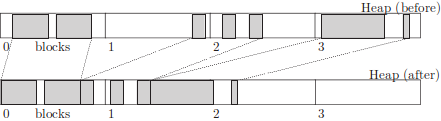
\includegraphics{figures/par_6}
  \caption
    [Συμπύκνωση με ολίσθηση μπλοκ.]
    {Συμπύκνωση με ολίσθηση μπλοκ. Ο Abuaiadh κ.ά ολισθαίνουν
     ολισθαίνουν ολόκληρα μπλοκ και όχι ξεχωριστά αντικείμενα.}
  \label{fig:par_6}
\end{figure}

Υπάρχουν δύο μειονεκτήματα όσον αφορά τον τρόπο που ο αλγόριθμος
συμπυκνώνει αντικείμενα. Πρώτον, πραγματοποιεί τρία περάσματα
στο σωρό. Δεύτερον, αντί να συμπυκνώσουν όλα τα ζωντανά αντικείμενα
στο ένα άκρο της παλαιάς γενεάς του σωρού, ο Flood κ.ά συμπυκνώνουν
την παλαιά γενεά σε $N$ πυκνά τμήματα, αφήνοντας $\lceil{\frac{N+1}{2}}\rceil$
κενά για εκχώρηση. Δε σπαταλάται χώρος σε κάθε συμπυκνωμένο τμήμα
εκτός ίσως για λόγους ευθυγράμμισης των αντικειμένων. Ωστόσο, αν
ο αριθμός των περιοχών ή νημάτων συμπύκνωσης είναι πολύ μεγάλος,
η εκχώρηση μεγάλων αντικειμένων στα νήματα τροποποιητές μπορεί
να καταστεί αδύνατη.

Ο Abuaiadh κ.ά \cite{DBLP:conf/oopsla/AbuaiadhOPS04} για να αντιμετωπίσουν
το πρώτο πρόβλημα υπολογίζουν μόνο και δεν αποθηκεύουν τις διευθύνσεις
προώθησης, χρησιμοποιώντας το bitmap σήμανσης και ένα διάνυσμα
μετατόπισης που αποθηκεύει τη νέα διεύθυνση του πρώτου ζωντανού
αντικειμένου σε κάθε μικρό μπλοκ του σωρού. Λύνουν το δεύτερο πρόβλημα
υπερ-διαμερίζοντας το σωρό σε έναν αριθμό σχετικά μεγάλες περιοχές.
Για παράδειγμα, προτείνουν το πλήθος των περιοχών να είναι τετραπλάσιο
του αριθμού των επεξεργαστών και η κάθε περιοχή να είναι τουλάχιστον
4 MB. Οι περιοχές του σωρού συμπυκνώνονται με τη σειρά. Tα νήματα
συμπύκνωσης ανταγωνίζονται για την απόκτηση μιας περιοχής χρησιμοιώντας
μια ατομική λειτουργία για να αυξήσουν έναν καθολικό μετρητή (ή
δείκτη). Αν η αύξηση είναι επιτυχής, το νήμα συμπύκνωσης έχει
αποκτήσει την περιοχή. Αν πάλι όχι, η συγκεκριμένη περιοχή βρίσκεται
στην κατοχή κάποιου άλλου νήματος συμπύκνωσης και το νήμα προσπαθεί
να αποκτήσει την επόμενη περιοχή. Ένας πίνακας αποθηκεύει δείκτες
προς την αρχή του ελεύθερου χώρου κάθε περιοχής. Αφού αποκτήσει
μια περιοχή για συμπύκνωση, ένα νήμα διεκδικεί μία περιοχή στην
οποία μπορεί να μετακινήσει αντικείμενα. Ένα νήμα αποκτά μια
περιοχή προσπαθώντας να γράψει την ειδική τιμή \textbf{null}
στο αντίστοιχο πεδίο του πίνακα. Τα νήματα συμπύκνωσης ποτέ δε
συμπυκνώνουν από ή προς μια περιοχή της οποίας ο αντίστοιχος
δείκτης στον πίνακα έχει την τιμή \textbf{null}, ενώ δε μεταφέρονται
αντικείμενα από κάποια περιοχή με μικρότερο αριθμό προς κάποια
περιοχή με μεγαλύτερο αριθμό. Η πρόοδος εξασφαλίζεται αφού ένα
νήμα μπορεί πάντοτε να συμπυκνώσει μια περιοχή στον εαυτό της.
Όταν ένα νήμα ολοκληρώσει τη συμπύκνωση μιας περιοχής, ενημερώνει
τον κατάλληλο δείκτη του πίνακα και στην περίπτωση που μια περιοχή
είναι γεμάτη, ο τελευταίος εξακολουθεί να έχει την τιμή \textbf{null}.

Ο Abuaiadh κ.ά εξερεύνησαν δύο τρόπους μετακίνησης αντικειμένων.
Η βέλτιστη συμπύκνωση με τον ελάχιστο κατακερματισμό προκύπτει
από την μετακίνηση ζωντανών αντικειμένων ξεχωριστά, όπως ακριβώς
περιγράφηκε πιο πάνω. Επειδή κάθε αντικείμενο ενός μπλοκ μετακινείται
σε μία θέση που εν μέρει προσδιορίζεται από το διάνυσμα μετατοπίσεων
για τον εν λόγω μπλοκ, τα αντικείμενα ενός μπλοκ δε διασκορπίζονται
μεταξύ δύο διαφορετικών περιοχών. Ο Abuaiadh κ.ά δοκίμασαν επίσης
να μειώσουν το χρόνο συμπύκνωσης θυσιάζοντας την ποιότητα της δια
μέσου της μετακίνησης ολόκληρων μπλοκ (256 bytes). Καθώς τα αντικείμενα
ενός χώρου μνήμης που εκχωρείται σειριακά έχουν την τάση να ζουν
και να πεθαίνουν σε συστάδες, ο Abuaiadh κ.ά υπολόγισαν πώς
η τεχνική αυτή μπορεί να μειώσει το συνολικό χρόνο συμπύκνωσης
κατά 20\% πληρώνοντας το κόστος της αύξησης του μεγέθους της
περιοχής συμπύκνωσης κατά ένα πολύ μικρό ποσοστό. Από την άλλη
πλευρά όμως, δεν είναι δύσκολη η επινόηση μιας περίπτωσης όπου
η τεχνική αυτή οδηγεί σε μηδενική συμπύκνωση.

Ο μηχανισμός υπολογισμού μόνο και όχι αποθήκευσης της διεύθυνσης
προώθησης ενός αντικειμένου υιοθετήθηκε αργότερα από τον αλγόριθμο
Compressor των Kermany και Petrank \cite{DBLP:conf/pldi/KermanyP06}.
Ο αλγόριθμος Compressor ωστόσο εισάγει κάποιες διαφορές. Πρώτον,
καθώς η δεύτερη φάση της συλλογής σαρώνει το bitmap σήμανσης,
υπολογίζει εκτός από το διάνυσμα μετατόπισης και ένα επιπλέον
βοηθητικό διάνυσμα, το οποίο δεικτοδοτείται από τις σελίδες προορισμού
των αντικειμένων. Σε κάθε θέση του βοηθητικού διανύσματος αποθηκεύεται
η αρχική διεύθυνση του πρώτου αντικειμένου που θα μετακινηθεί
στην αντίστοιχη σελίδα. Η συμπύκνωση καθεαυτή εκκινεί με την
ενημέρωση των ριζών.

Η δεύτερη διαφορά είναι πώς στη συνέχεια κάθε νήμα ανταγωνίζεται
για την απόκτηση μιας σελίδας-προς από το βοηθητικό διάνυσμα.
Μετά την επιτυχή προσπάθεια απόκτησης μιας σελίδας-προς, ένα
νήμα συμπύκνωσης αντιστοιχίζει την εικονική αυτή σελίδα σε μία
καινούρια φυσική σελίδα και ξεκινά να μεταφέρει αντικείμενα
με χρήση των διανυσμάτων σήμανσης και μετατόπισης και εκκινώντας
από τη διεύθυνση που υποδεικνύει το βοηθητικό διάνυσμα. Η απόκτηση
μιας νέας σελίδας-προς, στην οποία μπορεί να μεταφέρει αντικείμενα
επιτρέπει στον αλγόριθμο Compressor τη χρήση παράλληλων νημάτων
συμπύκνωσης. Εκ πρώτης όψεως, φαίνεται πώς ο Compressor είναι
αλγόριθμος συλλογής με αντιγραφή και όχι με σήμανση και εκκαθάριση.
Στην πραγματικότητα όμως πρόκειται για ένα συλλέκτη με σήμανση
και ολισθαίνουσα συμπύκνωση. Κάθε νήμα συμπύκνωσης διαχειρίζεται
κάθε ζεύγος από μια εικονική σελίδα-από και μια εικονική σελίδα-προς
με χρήση μίας φυσικής σελίδας μνήμης: όπως ακριβώς προσθέτει
μια αντιστοίχιση μεταξύ της εικονικής σελίδας-προς και μιας
καινούριας φυσικής σελίδας τη στιγμή της απόκτησης της σελίδας-προς,
με τον ίδιο τρόπο αφαιρεί μια αντιστοίχιση μεταξύ μιας εικονικής
σελίδας-από και της αντίστοιχης φυσικής σελίδας τη χρονική στιγμή
της ολοκλήρωσης της μεταφοράς των ζωντανών αντικειμένων από τη
σελίδα-προς.
 
Αυτή η σχεδίαση ελαχιστοποιεί την επιβάρυνση εξαιτίας του συγχρονισμού
των νημάτων συμπύκνωσης. Μόνο η προσπάθεια απόκτησης μιας σελίδας-προς
από το βοηθητικό διάνυσμα εκτελείται συγχρονισμένα από ένα νήμα
συμπύκνωσης. Αν η προσπάθεια είναι ανεπιτυχής, το νήμα προσπαθεί
να αποκτήσει τη σελίδα-προς στην οποία αντιστοιχεί η επόμενη
θέση του βοηθητικού διανύσματος. Ο τερματισμός της συμπύκνωσης
είναι εξίσου απλός: η εκτέλεση ενός νήματος συμπύκνωσης ολοκληρώνεται
όταν αυτό έχει εξετάσει και την τελευταία θέση του βοηθητικού
διανύσματος. 

\section{Ανακεφαλαίωση και θέματα προς εξέταση}
\subsection{Ορολογία}
Οι δημοσιεύσεις του 20ού αιώνα χρησιμοποιούν αυθαίρετα και
αδιακρίτως τους όρους παράλληλος, ταυτόχρονος και πραγματικού-χρόνου.
Από το 2000 ωστόσο, οι ερευνητές έχουν υιοθετήσει μία συνεπή
χρήση των όρων. Ένας παράλληλος συλλέκτης σκουπιδιών είναι ένας
συλλέκτης που χρησιμοποιεί πολλά νήματα συλλογής, τα οποία
εκτελούνται παράλληλα. Ο κόσμος μπορεί να διακόπτεται αλλά και
να μην διακόπτεται κατά τη διάρκεια εκτέλεσης των παράλληλων
νημάτων συλλεκτών. Με τον ίδιο τρόπο που είναι επιθυμητό να
επιτρέπεται σε πολλαπλά νήματα τροποποιητές να κάνουν χρήση
όλων των παράλληλων πόρων, η επίτρεψη της παράλληλης συλλογής
όταν η αρχιτεκτονική το επιτρέπει αποτελεί συνετή πράξη.

\subsection{Αξίζει η παραλληλοποίηση;}
Λαμβάνοντας υπόψη το νόμο του Amdahl \footnote{Ο νόμος του Amdahl
δηλώνει πώς η επιτάχυνση που προκύπτει από την παραλληλοποίηση
ενός προγράμματος εξαρτάται από το} προκύπτει το εύλογο ερώτημα
αν υπάρχει επαρκής δουλειά προς παραλληλοποίηση. Είναι εύκολο
να φανταστεί κανείς σενάρια που δεν προσφέρουν ευκαιρίες για
παραλληλοποίηση: ένα συνηθισμένο παράδειγμα τέτοιου σεναρίου
αποτελεί η εξιχνίαση μιας απλής συνδεδεμένης λίστας. Όπως
παρατηρεί ο Siebert \cite{DBLP:conf/iwmm/Siebert08}, υπάρχουν
πολλές ενδείξεις πώς οι πραγματικές εφαρμογές χρησιμοποιούν
ένα πολύ πιο πλούσιο ρεπερτόριο από δομές δεδομένων προσφέροντας
δυνατότητες παραλληλοποίησης υψηλού βαθμού. Εκτός από τη σήμανση,
οι υπόλοιπες δραστηριότητες της συλλογής σκουπιδιών προσφέρουν
εμφανώς περισσότερες δυνατότητες εκμετάλλευσης του παράλληλου
υλικού. Για παράδειγμα, η εκκαθάριση και η συμπύκνωση είναι
εγγενώς παραλληλοποιήσιμες διαδικασίες (παρότι η δεύτερη απαιτεί
λίγη παραπάνω προσοχή). Ακόμη και στη φάση της σήμανσης ωστόσο,
οι στοίβες και τα ενθυμούμενα σύνολα των νημάτων τροποποιητών
δύνανται να σαρώνονται παράλληλα και με μία μικρή επιβάρυνση
συγχρονισμού. Η παράλληλη εξιχνίαση του γράφου αντικειμένων
απαιτεί προσεκτικό σχεδιασμό όσον αφορά το χειρισμό των λιστών
εργασιών ούτως ώστε να περιορισθεί το κόστος συγχρονισμού και
ταυτόχρονα οι παράλληλοι πόροι του συστήματος να χρησιμοποιούνται
όσο το δυνατόν αποδοτικότερα.

\subsection{Στρατηγικές εξισορρόπησης φορτίου εργασίας}
Η αποδοτική παραλληλοποίηση της συλλογής απαιτεί προσεκτικό
συμβιβασμό μεταξύ της εξισορρόπησης του φορτίου εργασίας
μεταξύ των επεξεργαστών και του απαραίτητου συγχρονισμού.
Η εξισορρόπηση του φορτίου εργασίας εξασφαλίζει την αποτροπή
μιας κατάστασης όπου ορισμένοι επεξεργαστές εκτελούν όλες
τις εργασίες και κάποιοι άλλοι είναι αδρανείς. Ο συγχρονισμός
είναι απαραίτητος καθώς εξασφαλίζει την ακεραίοτητα τόσο των
ιδιωτικών δομών δεδομένων των νημάτων όσο και των καθολικών
δομών δεδομένων του σωρού.
 
Η γενική λύση ορίζει την ανάθεση στα νήματα συλλογής κβάντων
εργασίας τα οποία μπορούν να εκτελέσουν χωρίς περαιτέρω
συγχρονισμό. Η φθηνότερη λύση όσον αφορά το κόστος συγχρονισμού
αφορά τη στατική διαίρεση της εργασίας είτε κατά την εκκίνηση
του προγράμματος είτε ακριβώς πριν από κάθε κύκλο συλλογής.
Στην περίπτωση αυτή απαιτείται συντονισμός μεταξύ των παράλληλων
νημάτων απαιτείται μόνο για τον εντοπισμό του τερματισμού μιας
φάσης συλλογής. Ωστόσο η στατική διαμέριση μπορεί να μην οδηγήσει
σε ικανοποιητική εξισορρόπηση του φορτίου εργασίας. Το φορτίο
εργασίας μπορεί να εξισορροπισθεί επίσης υπερ-διαμερίζοντας
τη διαθέσιμη εργασία σε υποεργασίες και θέτοντας τα παράλληλα
νήματα να ανταγωνίζονται μεταξύ τους για την απόκτηση κβάντων
εργασίας από μια καθολική δεξαμενή καθώς και να επιστρέφουν
καινούρια κβάντα εργασίας σε αυτή. Η δεύτερη προσέγγιση έχει
εμφανώς μεγαλύτερο κόστος συγχρονισμού.

Συχνά βέβαια είναι δυνατή η εφαρμογή διαφορετικών στρατηγικών
εξισορρόπησης του φορτίου εργασιών σε διαφορετικές φάσεις ενός
κύκλου συλλογής. Η πληροφορία που γίνεται διαθέσιμη μετά το
πέρας μιας φάσης (συνήθως της φάσης σήμανσης) μπορεί να χρησιμοποιηθεί
προκειμένου να εκτιμηθεί μια δίκαιη διαίρεση της εργασίας των
επόμενων φάσεων ανάμεσα στα παράλληλα νήματα.
 
\subsection{Χειρισμός εξιχνίασης}
Η εξιχνίαση του σωρού περιλαμβάνει την κατανάλωση εργασίας
και την παραγωγή περαιτέρω εργασίας. Μια δομή δεδομένων, όπως
μια στοίβα ή μια ουρά είναι απαραίτητη για την καταγραφή
της εργασίας. Μια μοναδική, διαμοιραζόμενη δομή θα οδηγούσε
σε υψηλό κόστος συγχρονισμού και συνεπώς θα πρέπει να νήματα
να διατηρούν τις δικές τους ιδιωτικές δομές δεδομένων. Ωστόσο
η εξισορρόπηση του φορτίου εργασίας απαιτεί την ύπαρξη ενός
μηχανισμού μεταφοράς μονάδων εργασίας μεταξύ των νημάτων.
Η πρώτη απόφαση αφορά στην επιλογή του μηχανισμού. Δομές
δεδομένων που υποστηρίζουν κλοπή εργασίας μπορούν να χρησιμοποιηθούν
ώστε να επιτραπεί η μεταφορά μονάδων εργασίας μεταξύ των νημάτων.
Η ιδέα είναι η κοινή λειτουργία (ώθηση και εξώθηση στοιχείων
κατά την εξιχνίαση) να καταστεί όσο φθηνότερη (δηλαδή ασυγχρόνιστη)
γίνεται ενώ ταυτόχρονα επιτρέπονται λιγότερο συχνές λειτουργίες
(ασφαλής μεταφορά εργασίας μεταξύ των νημάτων). Ο Endo κ.ά
\cite{DBLP:conf/sc/EndoTY97} παρέχουν σε κάθε νήμα μία ιδιωτική
στοίβα και μία κλεπτόμενη ουρά εργασίας, ενώ ο Flood κ.ά
\cite{DBLP:conf/jvm/FloodDSZ01}
χρησιμοποιούν απλώς μια διπλά-τερματισμένη ουρά τόσο για τη
σήμανση όσο και για την κλοπή. Η τεχνική των γκρι πακέτων
\cite{DBLP:conf/pldi/OssiaBGKLO02}
διατηρεί μια καθολική δεξαμενή πακέτων εργασιών. Εδώ κάθε
νήμα ανταγωνίζεται για την απόκτηση ενός πακέτου εργασίας
από την καθολική δεξαμενή και επιστρέφει καινούρια εργασία
σε αυτή μέσω ενός φρέσκου πακέτου. Οι Cheng και Blelloch
\cite{DBLP:conf/pldi/ChengB01} λύνουν το πρόβλημα του συγχρονισμού των λειτουργιών
ώθησης και εξώθησης στοίβας χωρίζοντας την εξιχνίαση σε δύο
φάσεις που ονομάζουν δωμάτια. Η απλούστερη εκδοχή του αλγορίθμου
τους ορίζει πώς όλα τα νήματα βρίσκονται είτε στο δωμάτιο
ώθησης είτε στο δωμάτιο εξώθησης. Σε κάθε περίπτωση όλα τα
νήματα επιθυμούν να μετακινήσουν το δείκτη στοίβας προς την
ίδια κατεύθυνση και αυτό έχει ως αποτέλεσμα τη δυνατότητα
χρήσης μιας ατομικής λειτουργίας όπως η \textproc{FetchAndAdd}.

Η δεύτερη απόφαση αφορά το μέγεθος και τον τρόπο της μεταφερόμενης
εργασίας. Η ελάχιστη μεταφερόμενη μονάδα εργασίας είναι ένα
στοιχείο της στοίβας. Ωστόσο, η χρήση μικρών δομών δεδομένων
μπορεί να οδηγήσει στη διακίνηση μεγαλύτερου όγκου δεδομένων
μεταξύ των νημάτων. Στον παράλληλο, ταυτόχρονο και πραγματικού
χρόνου συλλέκτη του, o Siebert \cite{DBLP:conf/iwmm/Siebert10}
επιτρέπει σε έναν αδρανή επεξεργαστή να κλέψει ολόκληρη τη
δουλειά από έναν άλλον επεξεργαστή. Αυτή η απόφαση είναι συνετή
μόνο αν η περίπτωση να ξεμείνουν και οι υπόλοιποι επεξεργαστές
από δουλειά περίπου την ίδια χρονική στιγμή είναι σχεδόν
απίθανη. Μια συνήθης πρακτική είναι να μεταφέρεται ένα ενδιάμεσο
μέγεθος εργασίας ανάμεσα στα νήματα. Με τη χρήση γκρι πακέτων
σταθερού μεγέθους αυτό γίνεται αυτόματα. Μια άλλη επιλογή
είναι η μεταφορά της μισής ιδιωτικής στοίβας σήμανσης ενός
νήματος. Αν οι ιδιωτικές στοίβες σήμανσης έχουν σταθερό
μέγεθος, τότε απαιτείται και ένας μηχανισμός χειρισμού της
υπερχείλισης. Και αυτή η περίπτωση αντιμετωπίζεται αυτόματα
από την τεχνική των γκρι πακέτων: όταν ένα γεμάτο πακέτο
εξόδου γεμίζει μεταφέρεται στην καθολική και δεξαμενή και
λαμβάνεται ένα άδειο πακέτο από αυτή. Ο Flood κ.ά 
\cite{DBLP:conf/jvm/FloodDSZ01} χειρίζονται την υπερχείλιση
μέσω αντικειμένων κλάσεων στη γλώσσα Java, πληρώνοντας ένα
μικρό κόστος σε χώρο για κάθε κλάση.

Στο επίκεντρο της σχεδίασης των παραπάνω αλγορίθμων είναι ο
επεξεργαστής. Στρατηγικές όπου στο επίκεντρο της σχεδίασης
είναι η μνήμη και οι οποίες λαμβάνουν υπόψη τις θέσεις των
αντικειμένων στο σωρό είναι πιο συνήθεις σε αλγορίθμους για
συλλογή με παράλληλη αντιγραφή, όπου οι λίστες εργασίες
οργανώνονται ως ουρές Cheney. Τα ζητήματα σχεδίασης αφορούν:
\begin{inparaenum}[(i)]
\item το μέγεθος των μπλοκ (κβάντων εργασίας)
\item τη σειρά επεξεργασίας των μπλοκ καθώς και τον καθορισμό
      του ποια μπλοκ θα επιστραφούν στην καθολική δεξαμενή και
\item στην ιδιοκτησία ποιου νήματος βρίσκεται ένα αντικείμενο
\end{inparaenum}. 
Υπάρχουν δύο πτυχές όσον αφορά την επιλογή του μεγέθους των
μπλοκ. Πρώτον, κάθε μετακινών συλλέκτης πρέπει να διαθέτει
μια ιδιωτική περιοχή στο σωρό για την αντιγραφή αντικειμένων.
Το κομμάτι μνήμης που αντιστοιχεί στην περιοχή πρέπει να είναι
αρκετά μεγάλο ώστε να μειωθεί η συμφόρηση στο διαχειριστή
κομματιών που προκύπτει από τον ανταγωνισμό των νημάτων. Μεγάλο
μέγεθος κομματιών ωστόσο οδηγεί σε χαμηλή ποιότητα εξισορρόπησης
του φορτίου εργασίας και έτσι τα κομμάτια συνήθως διαιρούνται
περαιτέρω σε μπλοκ, τα οποία λειτουργούν ως κβάντα εργασίας
σε ένα συλλέκτη κατά Cheney. Δεύτερον, η απόφαση σχετικά με
το ποιο θα είναι το επόμενο αντικείμενο που θα επεξεργασθεί
επηρεάζει την τοπικότητα τόσο του συλλέκτη όσο και του τροποποιητή.
Και στις δύο περιπτώσεις φαίνεται προτιμότερο να διαλεχθεί
το επόμενο μη σαρωθέν αντικείμενο του μπλοκ εκχώρησης, επιστρέφοντας
ενδιάμεσα, μη σαρωθέντα ή και πλήρως σαρωθέντα μπλοκ στην
καθολική δεξαμενή. Η απόφαση μπορεί επίσης να βασισθεί στο
ποιος είναι ο επεξεργαστής που έχει τη μεγαλύτερη πιθανότητα
χρησιμοποίησης του αντικειμένου. Ο Ogasawara \cite{DBLP:conf/oopsla/Ogasawara09}
εισάγουν την έννοια ενός κυρίαρχου νήματος για να κατευθύνουν
την επιλογή του ποιος επεξεργαστής πρέπει να αντιγράψει ένα
αντικείμενο (και άρα σε ποια θέση αυτό θα αντιγραφεί).

\subsection{Συγχρονισμός χαμηλού επιπέδου}
Πολλές φορές εκτός από το συγχρονισμό λειτουργιών που αφορούν
τις δομές δεδομένων του συλλέκτη απαιτείται και ο συγχρονισμός
των λειτουργιών που δρουν σε κάθε ξεχωριστό αντικείμενο του
σωρού. Για παράδειγμα, δεν έχει σημασία αν ένα αντικείμενο
σημανθεί παραπάνω από μία φορές. Αν ωστόσο ο συλλέκτης χρησιμοποιεί
ένα ξεχωριστό διάνυσμα για την αποθήκευση των bits σήμανσης,
πρέπει να εξασφαλισθεί η ατομικότητα της τροποποίησης των
τελευταίων. Καθώς τα σύνολα εντολών των περισσότερων σύγχρονων
επεξεργαστών δεν παρέχουν εντολές για την ενημέρωση ενός συγκεκριμένου
bit σε μία λέξη μνήμης, η σήμανση ενός bit ενδέχεται να προκαλέσει
την αναμονή σε κάποιο βρόχο για την ατομική ενημέρωση ολόκληρου
του byte. Από την άλλη πλευρά, αν το bit σήμανσης αποθηκεύεται
στην επικεφαλίδα ενός αντικειμένου ή το διάνυσμα σήμανσης
χρησιμοποιεί ένα ξεχωριστό byte σήμανσης για κάθε αντικείμενο
δεν απαιτείται κανένας συγχρονισμός.

Ένας συλλέκτης αντιγραφής δεν πρέπει να 'σημάνει' (δηλαδή
αντιγράψει) ένα αντικείμενο περισσότερες από μία φορές καθώς
αυτό αλλάζει την τοπολογία του γράφου αντικειμένων και πιθανώς
έχει καταστροφικές συνέπειες για τον τροποποιητή. Η αντιγραφή
ενός αντικειμένου και η αποθήκευση της διεύθυνσης προώθησης
του από ένα νήμα αντιγραφής πρέπει να γίνεται αντιληπτή ως
μια μοναδική αδιαίρετη λειτουργία από τα υπόλοιπα νήματα
αντιγραφής. Ένα πλήθος από διαφορετικές τεχνικές έχει υιοθετηθεί
όσον αφορά το χειρισμό της διεύθυνσης προώθησης. Ένα νήμα
αντιγραφής μπορεί να επιχειρήσει να εγγράψει ατομικά μια ειδική
τιμή 'busy' στο πεδίο διεύθυνσης προώθησης ενός αντικειμένου
και αν τα καταφέρει, να αντιγράψει στη συνέχεια το αντικείμενο
και τέλος να ενημερώσει το πεδίο διεύθυνσης προώθησης με
τη διεύθυνση του αντιγράφου. Κάθε άλλο νήμα που θα διαβάσει
την τιμή 'busy' οφείλει να περιμένει μέχρις ότου διαβάσει
τη διεύθυνση προώθησης. Το κόστος συγχρονισμού μπορεί να
ελαττωθεί με τον έλεγχο του πεδίου διεύθυνσης προώθησης
πριν την προσπάθεια ατομικής εγγραφής της τιμής 'busy'
σε αυτό. Ένα νήμα αντιγραφής μπορεί ακόμη να αντιγράψει
ένα αντικείμενο αν το πεδίο διεύθυνσης προώθησης είναι
κενό, και στη συνέχεια να επιχειρήσει να εγγράψει ατομικά
στο πεδίο αυτό τη διεύθυνση του αντιγράφου, καταστρέφοντας
το αντικείμενο αντίγραφο αν η εγγραφή αποτύχει. Η αποδοτικότητα
της τελευταίας προσέγγισης θα εξαρτηθεί από τη συχνότητα
συγκρούσεων κατά την εγκατάσταση των διευθύνσεων προώθησης.

\subsection{Εκκαθάριση και συμπύκνωση}
Οι φάσεις της εκκαθάρισης και της συμπύκνωσης σαρώνουν γραμμικά
το σωρό (η συμπύκνωση μάλιστα περισσότερες της μίας φοράς). Και
οι δύο φάσεις είναι κατάλληλες για παραλληλοποίηση. Η απλούστερη
πολιτική εξισορρόπησης φορτίου διαμερίζει το σωρό σε τόσα τμήματα
όσα είναι οι επεξεργαστές. Η υιοθέτηση αυτής της προσέγγισης
ωστόσο μπορεί να οδηγήσει σε μη ομοιόμορφη εξισορρόπηση υπολογιστικού
φορτίου αν οι ποσότητες εργασίας των διαμερίσεων είναι άνισες.
Σε πρώτη προσέγγιση, η ποσότητα εργασίας είναι ανάλογη με τον
αριθμό των αντικειμένων σε μια διαμέριση. Η πληροφορία αυτή
είναι διαθέσιμη μετά το πέρας της φάσης σήμανσης και μπορεί
να χρησιμοποιηθεί για να διαμερισθεί ο σωρός σε όχι ισομεγέθη
τμήματα ώστε το καθένα από αυτά περιλαμβάνει περίπου την ίδια
ποσότητα εργασίας.

Ωστόσο, αυτή η στρατηγική προϋποθέτει πώς κάθε διαμέριση μπορεί
να επεξεργάζεται ανεξάρτητα από τις υπόλοιπες. Αυτό δεν είναι
αληθές αν η επεξεργασία μιας διαμέρισης μπορεί να καταστρέψει
πληροφορίες από τις οποίες εξαρτάται κάποια άλλη διαμέριση.
Για παράδειγμα, ένα νήμα ολισθαίνουσας συμπύκνωσης δεν μπορεί
να μετακινήσει αντικείμενα με τυχαία σειρά στον προορισμό τους
καθώς έτσι διακινδυνεύει να καταστρέψει ζωντανά αλλά όχι ακόμη
μετακινηθέντα αντικείμενα. Η λύση στο πρόβλημα να υπερ-διαμερισθεί
ο σωρός και τα νήματα ανταγωνίζονται για τις επόμενες διαμερίσεις
που θα χρησιμοποιήσουν (μία διαμέριση από την οποία θα μετακινήσουν
αντικείμενα και μία διαμέριση στην οποία θα τα μεταφέρουν).

\subsection{Τερματισμός}
Τέλος, ο τερματισμός οιασδήποτε φάσης συλλογής πρέπει να καθορίζεται
ορθά. Η χρήση παράλληλων νημάτων ασφαλώς και καθιστά τον εντοπισμό
του τερματισμού πιο πολύπλοκο. Το βασικό πρόβλημα είναι πώς ενώ
ένα νήμα επιχειρεί να προσδιορίσει εάν η φάση έχει ολοκληρωθεί,
ένα άλλο νήμα μπορεί να παράγει εργασία. Μια σωστή λύση στο
πρόβλημα είναι η ανάθεση του εντοπισμού του τερματισμού σε ένα
μόνο νήμα ενώ τα υπόλοιπα υποδεικνύουν ατομικά αν είναι απασχολημένα
ή όχι. Απαιτείται ιδιαίτερη προσοχή όσον αφορά το σχεδιασμό του
πρωτοκόλλου που ορίζει τη μετάβαση των διαφόρων μεταβλητών σημαιών
από την λογική τιμή 0 στη λογική τιμή 1 και αντίστροφα. Συστήματα
με μια καθολική δεξαμενή εργασιών από την άλλη πλευρά επιτρέπουν
σε περισσότερα του ενός νήματα να εντοπίζουν τον τερματισμό μιας
φάσης της συλλογής. 

\end{greek}

\begin{greek}
\chapter{Ταυτόχρονη συλλογή σκουπιδιών}\label{ch:conc}     

Οι βασικές αρχές της ταυτόχρονης συλλογής σκουπιδιών επινοήθηκαν
αρχικώς ως ένα μέσο για την μείωση των χρόνων παύσης για συλλογή
σκουπιδιών σε μονοεπεξεργαστικά συστήματα. Μέχρι στιγμής  έχουμε
υποθέσει πώς τα νήματα τροποποιητές παραμένουν αδρανοποιημένα
όσο εκτελείται συλλογή σκουπιδιών και πώς η συλλογή αυτή
ολοκληρώνεται στο σύνολό της πριν τα νήματα τροποποιητές
συνεχίσουν την εκτέλεσή τους.

Εκτός από την παράλληλη συλλογή σκουπιδιών που εξετάσαμε στο
προηγούμενο κεφάλαιο, ο χρόνος παύσης σε ένα μονοεπεξεργαστικό
μηχάνημα δύναται να μειωθεί με το να "σπάσει" ο κύκλος της 
συλλογής σκουπιδιών σε μικρότερα κβάντα και η εκτέλεση του
συλλέκτη να παρεμβάλλεται για κάθε ένα από αυτά τα κβάντα
χρόνου στην εκτέλεση του τροποποιητή. Η μέθοδος αυτή που
αναμιγνύει την εκτέλεση τροποποιητή και συλλέκτη είναι γνωστή
ως \textbf{αυξητική συλλογή σκουπιδιών}. Η τεχνική αυτή είναι
σημαντικά πολυπλοκότερη από ότι φαίνεται εκ πρώτης όψεως: ο
συλλέκτης παύει να εκτελείται πλέον ατομικά ως προς τον
τροποποιητή, με αποτέλεσμα ο γράφος προσβασιμότητας των
αντικειμένων πιθανώς να αλλάζει μεταξύ δύο διαδοχικών
δραστηριοποιήσεων αυτού. Επομένως, οι αυξητικοί συλλέκτες θα
πρέπει να έχουν έναν τρόπο να παρακολουθούν τις αλλαγές στο
γράφο των προσβάσιμων αντικειμένων ούτως ώστε αν χρειαστεί,
να επανεξετάσουν αντικείμενα η πεδία αυτών.

Παρότι αυτή η ανάμιξη δημιουργεί την ψευδαίσθηση πώς συλλέκτης
και τροποποιητής εκτελούνται ταυτόχρονα, αυτό δε συμβαίνει:
τα νήματα τροποποιητές αδρανοποιούνται κάθε φορά που εκτελείται
ο συλλέκτης. Στην περίπτωση που ο συλλέκτης αποτελείται από
περισσότερα του ενός νήματα, έχουμε να κάνουμε με
\textbf{παράλληλη αυξητική συλλογή σκουπιδιών}. Η σημαντικότερη
δυσκολία που προκύπτει αν επιτρέψουμε στα νήματα του συλλέκτη
να εκτελεστούν ταυτόχρονα με τα νήματα του τροποποιητή αφορά
στο να εξασφαλιστεί πώς ο συλλέκτης και ο τροποποιητής
διατηρούν σε κάθε χρονική στιγμή μία συνεπή εικόνα του σωρού.
Μια περίπτωση όπου μπορεί να προκύψει ασυνέπεια είναι εάν ο
τροποποιητής επιχειρήσει να πειράξει την τιμή ενός μερικώς
εξετασθέντος ή αντιγεγραμμένου αντικειμένου ή να αποκτήσει
πρόσβαση σε διάφορα μεταδεδομένα ταυτόχρονα με το συλλέκτη.
Ο απαιτούμενος συγχρονισμός μεταξύ συλλέκτη και τροποποιητή
δεν έρχεται χωρίς κόστος.
 
\begin{figure}
  \centering
  \begin{subfigure}{1.0\textwidth}
    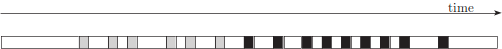
\includegraphics{figures/conc_1a}
    \caption{Αυξητική συλλογή σε σύστημα με μονοπύρηνο επεξεργαστή}
  \end{subfigure}

\begin{subfigure}[b]{1.0\textwidth}
  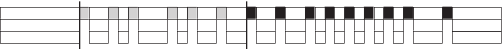
\includegraphics{figures/conc_1b}
  \caption{Αυξητική συλλογή σε σύστημα με πολυπύρηνο επεξεργαστή}
\end{subfigure}
  
  \begin{subfigure}[b]{1.0\textwidth}
    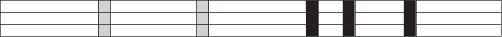
\includegraphics{figures/conc_1c}
    \caption{Παράλληλη αυξητική συλλογή}
  \end{subfigure}
  
  \begin{subfigure}[b]{1.0\textwidth}
    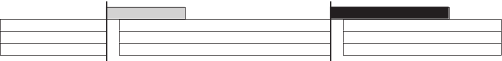
\includegraphics{figures/conc_1d}
    \caption{Σχεδόν-ταυτόχρονη συλλογή}
  \end{subfigure}
  
  \begin{subfigure}[b]{1.0\textwidth}
    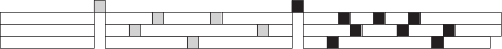
\includegraphics{figures/conc_1e}
    \caption{Σχεδόν-ταυτόχρονη αυξητική συλλογή}
  \end{subfigure}
  
  \begin{subfigure}[b]{1.0\textwidth}
    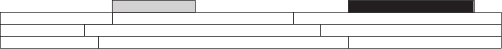
\includegraphics{figures/conc_1f}
    \caption{Εν-τη-πτήσει συλλογή}
  \end{subfigure}
  
  \begin{subfigure}[b]{1.0\textwidth}
    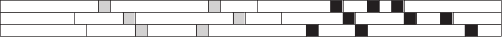
\includegraphics{figures/conc_1g}
    \caption{Εν-τη-πτήσει αυξητική συλλογή}
  \end{subfigure}
    
   \caption[Αυξητική και ταυτόχρονη συλλογή σκουπιδιών]
     {Αυξητική και ταυτόχρονη συλλογή σκουπιδιών. Κάθε μπάρα αναπαριστά μία εκτέλεση σε έναν επεξεργαστή.
      Οι έγχρωμες περιοχές αναπαριστούν διαφορετικούς κύκλους
      συλλογής σκουπιδιών.}
\end{figure}

Υποθέτοντας πώς ο συλλέκτης είναι μονονηματικός και ο
τροποποιητής πολυνηματικός, και πώς ο τροποποιητής
αδρανοποιείται για ένα πολύ σύντομο χρονικό διάστημα στην
αρχή του κύκλου εκτέλεσης του συλλέκτη, ώστε ο τελευταίος να
εξετάσει τις μεταβλητές-ρίζες των πρώτου, τότε έχουμε να
κάνουμε με \textbf{σχεδόν-ταυτόχρονη συλλογή σκουπιδιών}. Εάν
πάλι ο μονονηματικός συλλέκτης εκτελεστεί αυξητικά, όπως πριν,
έχουμε \textbf{σχεδόν-ταυτόχρονη αυξητική συλλογή σκουπιδιών}.
Αξίζει να προσέξουμε πώς στην τελευταία περίπτωση ο
μονονηματικός συλλέκτης μπορεί να εκτελείται σε διαφορετικό 
επεξεργαστή κάθε φορά.

Τέλος, αν θέλουμε να καταργήσουμε τελείως το χρόνο παύσης του
τροποποιητή και επιτρέψουμε στο μονονηματικό συλλέκτη να
εκτελεστεί πραγματικά ταυτόχρονα με αυτόν, τότε ανάλογα με το
αν αυτός εκτελείται συνεχόμενα ή αυξητικά, έχουμε
\textbf{εν-τη-πτήσει συλλογή σκουπιδιών} είτε
\textbf{εν-τη-πτήσει αυξητική συλλογή σκουπιδιών}. Δίνουμε
ιδιαίτερη έμφαση στην ορολογία καθώς μέχρι πρόσφατα οι όροι
παράλληλη, ταυτόχρονη, εν-τη-πτήσει και πραγματικού χρόνου
χρησιμοποιούνταν αυθαίρετα στη βιβλιογραφία.

\section{Ορθότητα ταυτόχρονης συλλογής}
Ένας ορθός ταυτόχρονος συλλέκτης πρέπει να έχει τις ακόλουθες
δύο ιδιότητες:

\begin{itemize}
\item η \textbf{ασφάλεια} απαιτεί τη διατήρηση τουλάχιστον
      όλων των ζωντανών αντικειμένων και
\item η \textbf{ζωντάνια} απαιτεί τον τερματισμό του κύκλου
      συλλογής.
\end{itemize}

\subsection{Η τριχρωματική αφαίρεση}
Η ορθότητα ταυτόχρονων συλλεκτών συνήθως αποδεικνύεται μέσω
αναλλοίωτων που βασίζονται στην τριχρωματική αφαίρεση και
πρέπει να διατηρούνται τόσο από το συλλέκτη όσο και από τον
τροποποιητή. Υπενθυμίζουμε πώς:

\begin{description}
  \item[Λευκά] αντικείμενα είναι εκείνα τα οποία δεν έχουν
    ακόμη ανακαλυφθεί από το συλλέκτη από την αρχή του
    τρέχοντος κύκλου συλλογής. Τα αντικείμενα που παραμένουν
    λευκά στο τέλος του κύκλου θεωρούνται μη-προσβάσιμα
    σκουπίδια.
  \item[Γκρι] αντικείμενα είναι εκείνα τα οποία έχουν ανακαλυφθεί
     από το συλλέκτη, αλλά ένα ή περισσότερα πεδία τους δεν
     έχουν εξετασθεί ακόμα (μπορεί να αναφέρονται σε λευκά
     αντικείμενα).
  \item[Μαύρα] αντικείμενα είναι εκείνα τα οποία έχουν ανακαλυφθεί
     από το συλλέκτη και των οποίων όλα τα πεδία έχουν εξετασθεί
     (και δεν περιέχουν δείκτες προς λευκά αντικείμενα). Τα
     μαύρα αντικείμενα δεν επανεξετάζονται εκτός και αν αλλάξει
     το χρώμα τους.
\end{description}

Ο συλλέκτης σκουπιδιών θεωρείται πώς μετακινεί ένα γκρι μέτωπο
κύματος, που είναι το σύνορο μεταξύ των μαύρων και των λευκών
αντικειμένων. Το πρόβλημα με την ταυτόχρονη εκτέλεση τροποποιητή
και συλλέκτη είναι πώς οι τελευταίοι ενδέχεται να μην μοιράζονται
μια συνεπή εικόνα του σωρού, καθώς το γκρι μέτωπο κύματος δεν
είναι πλέον αυστηρό σύνορο μεταξύ μαύρων και λευκών αντικειμένων.

Αν ο τροποποιητής εκτελείται ταυτόχρονα με το συλλέκτη και
τροποποιήσει πεδία αντικειμένων που βρίσκονται μπροστά από το
μέτωπο κύματος - γκρι αντικείμενα (των οποίων τα πεδία θα πρέπει
να σαρωθούν) ή λευκά αντικείμενα (τα οποία δεν έχουν ανακαλυφθεί 
ακόμη)-τότε δεν υπάρχει πρόβλημα καθώς ο συλλέκτης θα επανεξετάσει
τα αντικείμενα αυτά στο μέλλον (αν είναι ακόμη προσβάσιμα). 
Επίσης δεν υπάρχει πρόβλημα αν τροποποιεί αντικείμενα πίσω από
το μέτωπο κύματος-μαύρα αντικείμενα (των οποίων τα πεδία έχουν
ήδη σαρωθεί)-αρκεί να εισάγονται η διαγράφονται δείκτες μόνο
προς μαύρα ή γκρι αντικείμενα (για τα οποία ο συλλέκτης έχει
ήδη αποφανθεί πώς είναι προσβάσιμα). Όλες οι υπόλοιπες ενημερώσεις
δεικτών μπορεί να οδηγήσουν σε μία κατάσταση όπου τροποποιητής
και συλλέκτης έχουν διαφορετική εικόνα του σωρού.

Αυτό που σε κάθε περίπτωση πρέπει να αποφευχθεί είναι η εισαγωγή
ενός δείκτη προς κάποιο λευκό αντικείμενο στο πεδίο κάποιου μαύρου 
αντικειμένου, καθώς στην περίπτωση αυτή το πρώτο αντικείμενο, παρότι
προσβάσιμο, θα χαθεί (και έτσι θα συλλεχθεί εσφαλμένα).

Ο Wilson \cite{DBLP:conf/iwmm/Wilson92} αποδεικνύει πώς αντικείμενα
χάνονται αν κάποια στιγμή κατά την εξιχνίαση του γράφου αντικειμένων
ισχύουν ταυτόχρονα οι ακόλουθες δύο συνθήκες:

\begin{description}
  \item[Συνθήκη 1:] ο τροποποιητής αποθηκεύει σε ένα μαύρο αντικείμενο
                    ένα δείκτη προς ένα λευκό αντικείμενο και
  \item[Συνθήκη 2:] όλα τα μονοπάτια δια μέσου γκρι αντικειμένων προς
                    το λευκό αντικείμενο καταστρέφονται.
\end{description}

\subsection{Η ασθενής και η ισχυρή τριχρωματική αφαίρεση}
Για να αποφευχθεί η εσφαλμένη συλλογή ζωντανών αντικειμένων,
πρέπει να εξασφαλισθεί πώς οι δύο συνθήκες δεν μπορούν να
επικρατήσουν ταυτόχρονα. Για να μπορεί να εγγυηθεί ο συλλέκτης
πώς δε χάνει προσβάσιμα αντικείμενα, πρέπει να βεβαιωθεί πώς
βρίσκει όλα τα λευκά αντικείμενα προς τα οποία υπάρχει δείκτης
σε μαύρα αντικείμενα. Είναι αρκετό για ένα λευκό αντικείμενο
να είναι προσβάσιμο από κάποιο γκρι αντικείμενο είτε άμεσα
είτε έμμεσα μέσω μιας αλυσίδας λευκών αντικειμένων. Σε αυτήν
την περίπτωση η δεύτερη συνθήκη δεν επικρατεί ποτέ. Η ασθενής
τριχρωματική αναλλοίωτη που πρέπει να διατηρεί ο συλλέκτης
διατυπώνεται ως εξής:

\begin{description}
  \item[Η ασθενής τριχρωματική συνθήκη:] Όλα τα λευκά αντικείμενα
        προς τα οποία υπάρχει δείκτης σε κάποιο μαύρο αντικείμενο
        είναι προσβάσιμα από κάποιο γκρι αντικείμενο, είτε άμεσα,
        είτε μέσω μιας αλυσίδας λευκών αντικειμένων.
\end{description}

Οι ταυτόχρονοι συλλέκτες χωρίς αντιγραφή έχουν το πλεονέκτημα
πώς όλοι οι λευκοί δείκτες αυτόματα μετατρέπονται σε γκρι/μαύρους
όταν το αντικείμενο προς το οποίο δείχνουν σκιάζεται γκρι ή
μαύρο αντίστοιχα. Επομένως η παρουσία λευκών δεικτών στο εσωτερικό
μαύρων αντικειμένων δεν αποτελεί πρόβλημα, καθώς τα αντικείμενα
προς τα οποία δείχνουν, εφόσον τηρείται η ασθενής τριχρωματική
αναλλοίωτη θα σκιαστούν τελικώς γκρι ή μαύρα πριν το τέλος του
τρέχοντος κύκλου συλλογής.

Αντίθετα, οι ταυτόχρονοι συλλέκτες με αντιγραφή είναι πιο
περιορισμένοι καθώς διαθέτουν ρητά δύο αντίγραφα για κάθε
ζωντανό αντικείμενο στο τέλος κάθε κύκλου συλλογής (ένα
λευκό αντίγραφο στο χώρο-από και ένα μαύρο αντίγραφο στο
χώρο-προς), όπου τα λευκά αντικείμενα απορρίπτονται μαζί
με τα αντικείμενα σκουπίδια. Εξ 'ορισμού, ο συλλέκτης δεν
επισκέπτεται ξανά μαύρα αντικείμενα. Επομένως ένας ταυτόχρονος
συλλέκτης με αντιγραφή δεν πρέπει ποτέ να επιτρέψει ένα
πεδίο δείκτης ενός μαύρου αντικειμένου του χώρου-προς να
αναφέρεται προς ένα λευκό αντικείμενο του χώρου-από.
Η ισχυρή τριχρωματική αναλλοίωτη που πρέπει να διατηρεί
ένας τέτοιος συλλέκτης διατυπώνεται ως εξής:

\begin{description}
  \item[Η ισχυρή τριχρωματική συνθήκη:] Δεν υπάρχουν δείκτες
από μαύρα αντικείμενα προς λευκά αντικείμενα.
\end{description}

\subsection{Χρώμα τροποποιητή}
Κατά την κατηγοριοποίηση των αλγορίθμων ταυτόχρονης συλλογής
σκουπιδιών συχνά χρειάζεται να αναφερθούμε στο χρώμα των
αντικειμένων ριζών του τροποποιητή αντιμετωπίζοντας τον
τροποποιητή σαν αντικείμενο. Ένας τροποποιητής είναι γκρι
είτε αν δεν έχει πραγματοποιηθεί ακόμη εξιχνίαση από τις
ρίζες του είτε αν οι ρίζες του έχουν σαρωθεί και πρέπει
να σαρωθούν εκ νέου. Αυτό σημαίνει πώς οι ρίζες ενός γκρι
τροποποιητή μπορούν να αναφέρονται σε αντικείμενα όλων των
χρωμάτων. Ένας τροποποιητής είναι μαύρος αν έχει πραγματοποιηθεί
η εξιχνίαση από τις ρίζες του και αυτές δε θα σαρωθούν ξανά.
Υπό την ισχυρή τριχρωματική αναλλοίωτη αυτό σημαίνει πώς
οι ρίζες ενός μαύρου τροποποιητή μπορούν να αναφέρονται
μόνο σε μαύρα ή γκρι αντικείμενα. Υπό την ασθενή τριχρωματική
αναλλοίωτη, οι ρίζες ενός μαύρου τροποποιητή μπορούν να
αναφέρονται σε λευκά αντικείμενα, αρκεί τα τελευταία να είναι
προσβάσιμα από κάποιο γκρι αντικείμενο είτε έμμεσα είτε μέσω
μιας αλυσίδας λευκών αντικειμένων.

Το χρώμα του τροποποιητή έχει επιπτώσεις στον τερματισμό
ενός κύκλου συλλογής. Εξ 'ορισμού, αλγόριθμοι ταυτόχρονης
συλλογής σκουπιδιών πρέπει να σαρώσουν ξανά τις ρίζες ενός
γκρι τροποποιητή. Αυτό ενδέχεται να οδηγήσει σε καινούρια
εργασία εξιχνίασης αν βρεθεί ένας όχι μαύρος δείκτης. Όταν
η εξιχνίαση αυτή ολοκληρωθεί, οι ρίζες πρέπει να σαρωθούν
ξανά καθώς ο τροποποιητής μπορεί και πάλι στο ενδιάμεσο
να έχει αποθηκεύσει ένα μη μαύρο δείκτη κ.ό.κ. Στη χειρότερη
περίπτωση μπορεί να χρειαστεί να ανασταλεί η εκτέλεση όλων
των νημάτων τροποποιητών ώστε να σαρωθούν για μια τελευταία
φορά οι ρίζες τους.

Οι εν-τη-πτήσει συλλέκτες ξεχωρίζουν τα νήματα τροποποιητές
καθώς δεν αναστέλλουν την εκτέλεση όλων ταυτόχρονα για να
εξετάσουν τις ρίζες τους. Οι συλλέκτες αυτής της κατηγορίας
πρέπει να λειτουργήσουν με νήματα τροποποιητές διαφορετικών
χρωμάτων.

\subsection{Χρώμα εκχώρησης}
Το χρώμα του τροποποιητή επηρεάζει επίσης το χρώμα που
λαμβάνει ένα αντικείμενο κατά την εκχώρησή του, καθώς ο
ο δείκτης προς αυτό αποθηκεύεται στον τροποποιητή, ο οποίος
ανάλογα με το χρώμα του πρέπει να διατηρεί την ασθενή ή
ισχυρή τριχρωματική αναλλοίωτη. Το χρώμα εκχώρησης επηρεάζει
επίσης το πόσο γρήγορα θα απελευθερωθεί ένα αντικείμενο από
τη στιγμή που αυτό καθίσταται μη προσβάσιμο. Εάν ένα αντικείμενο
εκχωρείται ως μαύρο ή γκρι τότε δε θα ελευθερωθεί στη διάρκεια
του τρέχοντος κύκλου συλλογής (διότι τα μαύρα και γκρι αντικείμενα
θεωρούνται ζωντανά) ακόμη και εάν καταστεί μη προσβάσιμο.
Σε ένα γκρι τροποποιητή τα αντικείμενα μπορούν να εκχωρούνται
ως λευκά και έτσι να αποφεύγεται η χωρίς λόγο διατήρηση
νέων αντικειμένων. Αντίθετα, σε ένα μαύρο τροποποιητή νέα
αντικείμενα δεν μπορούν να εκχωρούνται ως λευκά εκτός και
αν διατηρείται η ασθενής τριχρωματική αναλλοίωτη και υπάρχει
κάποια εγγύηση πώς ο λευκός δείκτης θα αποθηκευθεί σε
ένα ζωντανό αντικείμενο που βρίσκεται μπροστά από το μέτωπο
κύματος και δε θα συλλεγεί εσφαλμένα. Τέλος, ένα καινούριο
αντικείμενο δεν περιέχει (ακόμη) δείκτες και συνεπώς
είναι πάντα ασφαλές να εκχωρείται ως μαύρο.

\section{Τεχνικές φράγματος για ταυτόχρονη συλλογή}
Σύμφωνα με τον Pirinen, \cite{DBLP:conf/iwmm/Pirinen98} οι
τεχνικές φράγματος που διατηρούν μία εκ των δύο τριχρωματικών
αναλλοίωτων βασίζονται σε έναν αριθμό από ενέργειες για να
διαχειρισθούν την εισαγωγή και διαγραφή δεικτών. Οι τεχνικές
αυτές μπορούν:
\begin{itemize}
\item Να αυξήσουν το μέγεθος του μετώπου κύματος, \textbf{σκιάζοντας}
  γκρι ένα αντικείμενο αν αυτό ήταν λευκό. Η σκίαση ενός γκρι
  ή μαύρου αντικειμένου δεν έχει κανένα αποτέλεσμα.
\item Να μετακινήσουν προς τα εμπρός το μέτωπο κύματος \textbf{σαρώνοντας}
  ένα αντικείμενο για να το χρωματίσουν μαύρο.
\item Να μετακινήσουν προς τα πίσω το μέτωπο κύματος \textbf{αντιστρέφοντας}
  το χρώμα ενός αντικειμένου από μαύρο σε γκρι.
\end{itemize}

\subsection{Τεχνικές γκρι τροποποιητή}
Αρχικά παρουσιάζουμε προσεγγίσεις που λειτουργούν με γκρι τροποποιητή.
Όλες αυτές οι τεχνικές διατηρούν την ισχυρή αναλλοίωτη χρησιμοποιώντας
ένα \textbf{φράγμα εισαγωγής} κατά την εγγραφή αναφορών στο σωρό για
να αποτρέψουν την αποθήκευση λευκών δεικτών σε μαύρα αντικείμενα.
Καθώς ο τροποποιητής είναι γκρι, δεν απαιτείται φράγμα εγγραφής.

\begin{itemize}
  \item Το φράγμα εγγραφής του Steele, \cite{DBLP:journals/cacm/Steele75} το
    οποίο φαίνεται στον αλγόριθμο~\ref{alg:conc_1} παρουσιάζει
    τη μεγαλύτερη ακρίβεια ανάμεσα σε όλες τις τεχνικές απλώς επειδή
    σημειώνει το αντικείμενο προέλευσης υπό τροποποίηση. Δε μεταβάλλει
    καμία απόφαση όσον αφορά την προσβασιμότητα ενός αντικειμένου, αλλά
    προκαλεί την μετακίνηση του μετώπου κύματος προς τα πίσω αλλάζοντας
    το χρώμα του τροποποιημένου μαύρου αντικειμένου από μαύρο σε γκρι.
    Αναβάλλει την απόφαση σχετικά με την προσβασιμότητα του λευκού
    αντικειμένου προορισμού μέχρις ότου το μαύρο αντικείμενο προέλευσης
    σαρωθεί εκ νέου (ο εισαχθείς δείκτης ενδέχεται να έχει διαγραφεί
    στο ενδιάμεσο). Η ακρίβεια αυτή έρχεται εις βάρος της προόδου,
    καθώς το μέτωπο κύματος μετακινείται προς τα πίσω.

   \item Ο Boehm κ.ά. \cite{DBLP:conf/pldi/BoehmDS91} υλοποίησαν μια
   παραλλαγή του φράγματος εγγραφής του Steele η οποία αγνοεί το χρώμα του
   εισαγόμενου δείκτη, όπως φαίνεται στον αλγόριθμο~\ref{alg:conc_1}.
   Αρχικά υλοποίησαν αυτό το φράγμα χρησιμοποιώντας
   τα βρώμικα bits της εικονικής μνήμης για να καταγράφουν τις
   τροποποιημένες σελίδες χωρίς να χρειάζεται έτσι οι λειτουργίες
   εγγραφής πεδίων αντικειμένων του σωρού να παρακολουθούνται σε επίπεδο
   λογισμικού. Η αρχική υλοποίηση του φράγματος μάλιστα δεν ήλεγχε
   πώς το αντικείμενο προέλευσης είναι μαύρο, καθιστώντας το φράγμα
   λιγότερο ακριβές. Ο τερματισμός της συλλογής γινόταν με παύση
   του κόσμου οπότε και οι βρώμικες σελίδες σαρώνονταν εκ νέου.

  \item Ο Dijkstra κ.ά. \cite{DBLP:conf/ac/DijkstraLMSS75,
   DBLP:journals/cacm/DijkstraLMSS78} σχεδίασαν ένα φράγμα εγγραφής
   (αλγόριθμος~\ref{alg:conc_1} λιγότερο
   ακριβές από το αντίστοιχο του Steele: το αντικείμενο προορισμού
   του εισαγόμενου δείκτη σκιάζεται ως προσβάσιμο (μη λευκό) παρότι
   ο δείκτης μπορεί στη συνέχεια να διαγραφεί. Αυτή η απώλεια
   ακρίβειας συμβάλλει στην πρόοδο καθώς το μέτωπο κύματος
   μετακινείται προς τα εμπρός. Η αρχική μάλιστα υλοποίηση του
   φράγματος ήταν ακόμη λιγότερο ακριβής καθώς το αντικείμενο
   προορισμού του εισαγόμενου δείκτη σκιαζόταν χωρίς να ελέγχεται
   πώς το χρώμα του αντικειμένου προέλευσης είναι μαύρο. Η παράλειψη
   αυτού του ελέγχου επιτρέπει τη χαλάρωση της απαίτησης για ατομική
   εκτέλεση όλου του φράγματος εγγραφής, υπό την προϋπόθεση βέβαια
   πώς οι ξεχωριστές λειτουργίες της αποθήκευσης και της σκίασης
   εκτελούνται ατομικά.
\end{itemize}

\subsection{Τεχνικές μαύρου τροποποιητή}
Οι πρώτες δύο προσεγγίσεις εφαρμόζουν αυξητική ενημέρωση για
τη διατήρηση της ισχυρής αναλλοίωτης χρησιμοποιώντας ένα φράγμα
ανάγνωσης για να αποτρέψουν τον τροποποιητή από την απόκτηση
λευκών δεικτών (δηλαδή να αποτρέψουν την εισαγωγή ενός λευκού
δείκτη σε ένα μαύρο τροποποιητή). Η τρίτη προσέγγιση χρησιμοποιεί
ένα \textbf{φράγμα διαγραφής} στις λειτουργίες εγγραφής δεικτών
στο σωρό για τη διατήρηση της ασθενούς αναλλοίωτης. Υπό την
ασθενή τριχρωματική αναλλοίωτη ένας μαύρος τροποποιητής μπορεί
να διατηρεί λευκούς δείκτες: είναι μαύρος καθώς δεν απαιτείται
η εκ νέου σάρωση των ριζών του και έτσι μπορεί να φορτώνει
τιμές δεικτών προς λευκά αντικείμενα, αφού το φράγμα εγγραφής
προστατεύει τα τελευταία από μια πιθανή διαγραφή.

\begin{itemize}
  \item Ο Baker \cite{DBLP:journals/cacm/Baker78} χρησιμοποίησε
    το φράγμα ανάγνωσης που φαίνεται στον αλγόριθμο~\ref{alg:conc_2}. Η
    προσέγγισή του είναι λιγότερο ακριβής από την προσέγγιση του
    Dijkstra κ.ά. καθώς εσφαλμένα διατηρεί αντικείμενα (που θα
    ήταν λευκά) απλώς επειδή κάποιο νήμα τροποποιητής φορτώνει
    τις τιμές δεικτών προς αυτά κατά τη διάρκεια ενός κύκλου
    συλλογής (σε αντίθεση με λευκά αντικείμενα που εισάγονται
    πίσω από το μέτωπο κύματος και τα οποία πρέπει να διατηρηθούν).
    Το φράγμα ανάγνωσης του Baker σχεδιάσθηκε αρχικώς για ένα
    συλλέκτη αντιγραφής, όπου η ενέργεια της σκίασης αντιγράφει
    ένα αντικείμενο από το χώρο-από στο χώρο-προς και έτσι η
    ρουτίνα \textproc{shade} επιστρέφει τη διεύθυνση του αντιγράφου
    του αντικειμένου στο χώρο-προς. 
  \item Ο Appel κ.ά. \cite{DBLP:conf/pldi/AppelEL88} υλοποίησαν
    μία λιγότερο ακριβή παραλλαγή του φράγματος ανάγνωσης του
    Baker, (αλγόριθμος~\ref{alg:conc_2} χρησιμοποιώντας μηχανισμούς
    προστασίας σελίδων εικονικής μνήμης για την παγίδευση των
    προσβάσεων νημάτων τροποποιητών σε γκρι σελίδες με αποτέλεσμα
    να μη χρειάζεται η παρακολούθηση των λειτουργιών ανάγνωσης σε
    επίπεδο λογισμικού. Μια παγιδευμένη πρόσβαση μπορεί να
    ολοκληρωθεί μετά τη σάρωση της αντίστοιχης σελίδας (και την
    άρση του αποκλεισμού της). Αυτό το φράγμα ανάγνωσης μπορεί
    επίσης να χρησιμοποιηθεί και από ένα ταυτόχρονο συλλέκτη
    αντιγραφής αφού η σάρωση θα προωθήσει τυχόν πεδία δείκτες
    προς αντικείμενα του χώρου-προς του αντικειμένου προέλευσης.   
  \item Οι Abraham και Patel \cite{DBLP:conf/icpp/AbrahamP87},
    και ο Yuasa \cite{DBLP:journals/jss/Yuasa90} σχεδίασαν
    ανεξάρτητα το φράγμα διαγραφής που φαίνεται στον αλγόριθμο~\ref{alg:conc_2}.
    Αυτό το φράγμα διαγραφής παρουσιάζει τη μικρότερη
    ακρίβεια από όλες τις τεχνικές καθώς διατηρεί κάθε μη
    προσβάσιμο αντικείμενο προς το οποίο ο τελευταίος δείκτης
    διαγράφηκε κατά τη διάρκεια του κύκλου συλλογής. 
\end{itemize}

\begin{algorithm}
  \caption{Φράγματα γκρι τροποποιητή}
  \label{alg:conc_1}
  \subcaption{\centering Φράγμα εγγραφής του Steele}%\label{alg:conc_1a}
  \hrulefill
  \begin{algorithmic}[1]
    \Procedure{Write}{$src$, $i$, $ref$}
      \State \textbf{atomic}
      \State $src[i] \gets ref$
      \If{\Call{isBlack}{$src$}}
        \If{\Call{isWhite}{$ref$}}
          \State \Call{revert}{$src$}
        \EndIf
      \EndIf
    \EndProcedure
  \end{algorithmic}
  \hrulefill
  \subcaption{\centering Φράγμα εγγραφής του Boehm κ.ά}%\label{alg:conc_1b}
  \hrulefill
  \begin{algorithmic}[1]
    \Procedure{Write}{$src$, $i$, $ref$}
      \State \textbf{atomic}
      \State $src[i] \gets ref$
      \If{\Call{isBlack}{$src$}}
        \State \Call{revert}{$src$}
      \EndIf
    \EndProcedure
  \end{algorithmic}
  \hrulefill
  \subcaption{\centering Φράγμα εγγραφής του Dijkstra κ.ά}%\label{conc_1c}
  \hrulefill
  \begin{algorithmic}[1]
    \Procedure{Write}{$src$, $i$, $ref$}
      \State \textbf{atomic}
      \State $src[i] \gets ref$
      \If{\Call{isBlack}{$src$}}
        \State \Call{shade}{$src$}
      \EndIf
    \EndProcedure
  \end{algorithmic}
\end{algorithm}

\begin{algorithm}
  \caption{Φράγματα μαύρου τροποποιητή}
  \label{alg:conc_2}
  \subcaption{\centering Φράγμα ανάγνωσης του Baker}%\label{conc_2a}
  \hrulefill
  \begin{algorithmic}[1]
    \Function{Read}{$src$, $i$}
      \State \textbf{atomic}
      \State $ref \gets src[i]$
      \If{\Call{isGrey}{$src$}}
          \State $ref \gets$ \Call{shade}{$src$}
      \EndIf
      \State \Return{$ref$}
    \EndFunction
  \end{algorithmic}
  \hrulefill
  \subcaption{\centering Φράγμα ανάγνωσης του Appel κ.ά}%\label{conc_2b}
  \hrulefill
  \begin{algorithmic}[1]
    \Function{Read}{$src$, $i$}
      \State \textbf{atomic}
      \State $src[i] \gets ref$
      \If{\Call{isGrey}{$src$}}
        \State \Call{scan}{$src$}
      \EndIf
      \State \Return{$src[i]$}
    \EndFunction
  \end{algorithmic}
  \hrulefill
  \subcaption{\centering Φράγμα εγγραφής των Abraham κ.ά / Yuasa}%\label{conc_2c}
  \hrulefill
  \begin{algorithmic}[1]
    \Procedure{Write}{$src$, $i$, $ref$}
      \State \textbf{atomic}
      \If{\Call{isGrey}{$src$} \textbf{or} \Call{isWhite}{$src$}}
        \State \Call{shade}{$src[i]$}
      \EndIf
      \State $src[i] \gets ref$
    \EndProcedure
  \end{algorithmic}
\end{algorithm}


\section{Ταυτόχρονη σήμανση και εκκαθάριση}
Στην ενότητα αυτή εξετάζουμε την
\textbf{ταυτόχρονη συλλογή με σήμανση και εκκαθάριση}. Όπως
είδαμε και πριν, το πιο σημαντικό θέμα όσον αφορά έναν
ταυτόχρονο συλλέκτη είναι η εξασφάλιση της ορθότητας.
Συλλέκτης και τροποποιητής οφείλουν να συνεργάζονται
προκειμένου να διαβεβαιώσουν πώς μοιράζονται μια συνεπή
εικόνα της μνήμης του σωρού. Ο τροποποιητής από την πλευρά
του οφείλει να αποτρέπει ζωντανά αντικείμενα να μην είναι
ορατά στο συλλέκτη, ενώ ένας συλλέκτης που μετακινεί
αντικείμενα οφείλει να εξασφαλίζει πώς ο συλλέκτης
χρησιμοποιεί τις σωστές διευθύνσεις των μετακινηθέντων
αντικειμένων.

Οι ταυτόχρονοι συλλέκτες με σήμανση και εκκαθάριση είναι οι
απλούστεροι από όλους τους ταυτόχρονους συλλέκτες. Καθώς δε
μεταβάλλουν πεδία δείκτες, ο τροποποιητής μπορεί ελεύθερα
να διαβάζει τις τιμές δεικτών χωρίς να χρειάζεται να
προστατευθεί από το συλλέκτη. Δεν υπάρχει επομένως εγγενής
ανάγκη για φράγμα ανάγνωσης όταν χρησιμοποιείται μη μετακινών
συλλέκτης. Ειδάλλως, η χρήση φράγματος ανάγνωσης για τη
διατήρηση της ισχυρής αναλλοίωτης σε ένα σύστημα με συλλέκτη
που δεν μετακινεί αντικείμενα θεωρείται πολύ ακριβή, καθώς οι
αναγνώσεις δεδομένων του σωρού από τον τροποποιητή είναι πολύ
συχνότερες από ότι οι εγγραφές. Για παράδειγμα, ο Zorn \cite{DBLP:conf/lfp/Zorn90}
μέτρησε και υπολόγισε το ποσοστό των φορτώσεων και αποθηκεύσεων
δεικτών στο σύστημα SPUR LISP από 13\% έως 15\% και 4\%
αντίστοιχα. Η εξαίρεση στον παραπάνω γενικό κανόνα προκύπτει
όταν τεχνικές βελτιστοποιήσεων του μεταγλωττιστή χρησιμοποιούνται
για να εξαλείψουν τα περιττά φράγματα, όπως από το Hosking κ.ά. \cite{DBLP:conf/oopsla/HoskingC99}
και τους Zee και Rinard \cite{DBLP:conf/oopsla/ZeeR02},
ή για να ενσωματώσουν ένα τμήμα του έργου των φραγμάτων στο ήδη
υπάρχον κόστος που αφορά τον έλεγχο των δεικτών έναντι της ειδικής τιμής \textbf{null},
όπως από το Bacon κ.ά. \cite{DBLP:conf/lctrts/BaconCR03}. Γι αυτό το λόγο οι
ταυτόχρονοι συλλέκτες με σήμανση και εκκαθάριση συνήθως 
χρησιμοποιούν το φράγμα αυξητικής ενημέρωσης του Dijkstra 
\cite{DBLP:conf/ac/DijkstraLMSS75,DBLP:journals/cacm/DijkstraLMSS78},
είτε το φράγμα εγγραφής εισαγωγής του Steele  \cite{DBLP:journals/cacm/Steele75},
είτε το φράγμα εγγραφής εισαγωγής του Boehm κ.ά. \cite{DBLP:conf/pldi/BoehmDS91},
είτε το φράγμα εγγραφής διαγραφής του Yuasa \cite{DBLP:journals/jss/Yuasa90}.

\subsection{Αρχικοποίηση}
Αντί να επιτρέπεται η εκτέλεση του τροποποιητή μέχρις ότου η μνήμη να εξαντληθεί, οι ταυτόχρονοι 
συλλέκτες μπορούν να εκτελούνται ακόμη και όταν ο τροποποιητής ακόμα μπορεί να δεσμεύει μνήμη 
προς δημιουργία αντικειμένων. Αν μία συλλογή  ενεργοποιηθεί πολύ αργά, ενδέχεται να μην υπάρχει 
επαρκής μνήμη για την ικανοποίηση ενός αιτήματος εκχώρησης, στην οποία περίπτωση θα καθυστερήσει 
η εκτέλεση του τροποποιητή μέχρις ότου τελειώσει ο κύκλος συλλογής. Τη στιγμή που εκκινεί ο 
κύκλος συλλογής, η ρυθμαπόδοση σταθερής κατάστασης του συλλέκτη πρέπει να επαρκεί για την 
ολοκλήρωση του κύκλου πριν εξαντληθεί η μνήμη από τον τροποποιητή και να επιδρά στη ρυθμαπόδοση 
του τελευταίου το ελάχιστο δυνατό. Το πότε και πώς θα ενεργοποιηθεί ένας κύκλος συλλογής 
εξασφαλίζοντας τη διαθεσιμότητα επαρκούς μνήμης για την ικανοποίηση των αιτημάτων του τροποποιητή 
και ενώ εκτελείται ο συλλέκτης, καθώς και το πότε ο κύκλος θα τελειώσει ούτως ώστε η μνήμη από
τα σκουπίδια να ανακτηθεί εξαρτώνται από τη δρομολόγηση εργασιών συλλογής παράλληλα με την 
εκτέλεση του τροποποιητή.

Ο αλγόριθμος~\ref{alg:conc_3} απεικονίζει την αλληλουχία ενεργειών κατά την εκχώρηση μνήμης στον 
τροποποιητή για έναν ταυτόχρονο συλλέκτη με σήμανση και εκκαθάριση ο οποίος δρομολογεί ένα 
ποσό έργου συλλογής αυξητικά σε κάθε εκχώρηση μνήμης μέσω της διαδικασίας \textenglish{\textproc{collectEnough}}. 
Η συνάρτηση \textenglish{\textproc{behind}} αποφασίζει σχετικά με το πότε και πόσο έργο συλλογής πρέπει να 
εκτελεστεί, εξασφαλίζοντας πώς ο τροποποιητής δεν βρίσκεται πολύ μπροστά από το συλλέκτη ώστε η 
συνάρτηση \textenglish{\textproc{allocate}} να μην μπορεί να ικανοποιήσει αιτήματα μνήμης.

Ο αλγόριθμος~\ref{alg:conc_4} δείχνει τι ακριβώς συμβαίνει όταν δρομολογείται η εκτέλεση έργου 
συλλογής. Η αρχικά κενή λίστα εργασιών γεμίζει με αναφορές προς αντικείμενα προς τα οποία δείχνουν 
οι ρίζες. Υποθέτοντας πώς η εξέταση των ριζών σημαίνει την αναστολή λειτουργίας και εξέταση όλων 
των νημάτων τροποποιητών, σε αυτό το σημείο κάνενα νήμα τροποποιητής δεν περιλαμβάνει κάποια 
λευκή αναφορά. Επομένως έχουμε έναν σχεδόν ταυτόχρονο τρόπο λειτουργίας, με μία μικρή φάση παύσης 
για την αρχικοποίηση της συλλογής. Τα γκρι πλέον αντικείμενα ρίζες αναπαριστούν το αρχικό μέτωπο 
κύματος από το οποίο θα συνεχίσει η εξερεύνηση του γράφου των αντικειμένων. Εφόσον οι ρίζες τους
έχουν εξετασθεί, τα νήματα τροποποιητές μπορούν πλέον να συνεχίσουν είτε ως μαύρα (εφόσον δεν 
έχουν λευκές αναφορές) είτε ως γκρι, ανάλογα με τα φράγματα τροποποίησης που είναι σε χρήση.

\begin{algorithm}
  \caption{Σχεδόν-ταυτόχρονη σήμανση και εκκαθάριση: εκχώρηση}
  \label{alg:conc_3}
  \begin{algorithmic}[1]
    \Function{New}{\null}
      \State \Call{collectEnough}{\null}
      \State $ref \gets$ \Call{allocate}{\null} \Comment{must initialize black if collector is black}
      \If{$ref = \textbf{null}$}
        \State error ''Out of memory''
      \EndIf
      \State \Return{$ref$}
    \EndFunction
    \Statex
    \Function{collectEnough}{\null}
      \State \textbf{atomic}
      \While{\Call{behind}{\null}}
        \If{\textbf{not} \Call{markSome}{\null}}
          \State \Return{null}
        \EndIf
      \EndWhile
    \EndFunction
  \end{algorithmic}
\end{algorithm}

Η αναστολή της λειτουργίας των νημάτων τροποποιητών ενδέχεται να οδηγήσει σε απαράδεκτες
παύσεις. Η χρήση γκρι φραγμάτων τροποποίησης καθιστά εφικτή την ενεργοποίηση των φραγμάτων και την 
αναβολή της εξέτασης όλων των ριζών, η οποία πραγματοποιείται αργότερα και ενώ ταυτόχρονα εκτελούνται 
τα νήματα τροποποιητές. 

\subsection{Τερματισμός σήμανσης}
Ο τερματισμός της φάσης σήμανσης για ένα μαύρο τροποποιητή είναι μία σχετικά απλή διαδικασία και 
συμβαίνει όταν δεν υπάρχουν πλέον γκρι αντικείμενα στη λίστα εργασιών. Σε αυτό το σημείο, θεωρώντας 
ακόμη και την ασθενή τριχρωματική αναλλοίωτη ο τροποποιητής μπορεί να περιλαμβάνει μόνο μαύρες 
αναφορές, καθώς δεν υπάρχουν λευκά αντικείμενα προσβάσιμα από γκρι αντικείμενα (δεν υπάρχουν καθόλου 
γκρι αντικείμενα). Καθώς ο τροποποιητής είναι μαύρος, δεν απαιτείται η επανεξέταση των ριζών του.

Ο τερματισμός της φάσης σήμανσης για έναν γκρι τροποποιητή είναι λίγο πιο περίπλοκος, καθώς ο 
τροποποιητής μπορεί να έχει αποκτήσει λευκούς δείκτες από τη στιγμή που εξετάστηκαν οι ρίζες του για 
την αρχικοποίηση της συλλογής. Επομένως οι ρίζες ενός γκρι τροποποιητή πρέπει να επανεξετασθούν πριν 
η φάση σήμανσης τερματιστεί. Εάν η επανεξέταση δεν ανακαλύψει φρέσκα γκρι αντικείμενα, τότε η φάση 
της σήμανσης τερματίζεται και εκκινεί η φάση της εκκαθάρισης. Η τελευταία μπορεί να είναι πρόθυμη ή 
οκνηρή. 

\begin{algorithm}
  \caption{Σχεδόν-ταυτόχρονη σήμανση}
  \label{alg:conc_4}
  \begin{algorithmic}[1]
    \State \textbf{shared} $worklist \gets empty$
    \Statex
    \Function{markSome}{\null}
      \If{\Call{isEmpty}{$worklist$}} \Comment{initiate collection}
        \State \Call{scan}{$Roots$} \Comment{invariant: collector holds no white references}
        \If{\Call{isEmpty}{$worklist$}} \Comment{invariant: no more grey references}
          \State /* marking terminates */
          \State \Call{sweep}{\null} \Comment{lazy or eager sweep}
          \State \Return{\textbf{false}} \Comment{terminate marking}
        \EndIf
      \EndIf
      \State /* collection continues */
      \State $ref \gets$ \Call{remove}{$worklist$}
      \State \Call{scan}{$ref$} \Comment{continue marking, if still behind}
      \State \Return{\textbf{true}}
    \EndFunction
    \Statex
    \Procedure{shade}{$ref$}
      \If{\textbf{not} \Call{isMarked}{\null}}
        \State \Call{setMarked}{$ref$}
        \State \Call{add}{$worklist$, $ref$}
      \EndIf
    \EndProcedure
    \Statex
    \Procedure{scan}{$ref$}
      \ForAll{$fld \; \textbf{in} \; Pointers(ref)$}
        \State $child \gets *fld$
        \If{$child \neq \textbf{null}$}
          \State \Call{shade}{$child$}
        \EndIf
      \EndFor
    \EndProcedure
    \Statex
    \Function{revert}{$ref$}
      \State \Call{add}{$worklist$, $ref$}
    \EndFunction
    \Statex
    \Function{isWhite}{$ref$}
      \State \Return{\textbf{not} \Call{isMarked}{$ref$}}
    \EndFunction
    \Statex
    \Function{isGrey}{$ref$}
      \State \Return{$ref \textbf{in} worklist$}
    \EndFunction
    \Statex
    \Function{isBlack}{$ref$}
      \State \Return{\Call{isMarked}{$ref$} \textbf{and} \textbf{not} \Call{isGrey}{$ref$}}
    \EndFunction
  \end{algorithmic}
\end{algorithm}

\subsection{Ταυτόχρονη σήμανση και ταυτόχρονη εκκαθάριση}
Μέχρι στιγμής έχουμε θεωρήσει την εκτέλεση μόνο της φάσης
της σήμανσης ταυτόχρονα με τον τροποποιητή και πως η φάση
της εκκαθάρισης έπεται αυτής σειριακά. Εάν η εκκαθάριση
είναι οκνηρή, αιτήματα εκχώρησης μνήμης από τον τροποποιητή
ενδέχεται να ενεργοποιούν την ταυτόχρονη εκκαθάριση που
αντιστοιχεί στη σήμανση του προηγούμενου κύκλου συλλογής
και ενώ ήδη ένας νέος κύκλος συλλογής βρίσκεται στην επόμενη
φάση σήμανσης. Το γεγονός αυτό μπορεί να προκαλέσει σύγχυση
όσον αφορά τα χρώματα των αντικειμένων. Θα πρέπει με κάποιο
τρόπο να μπορούν να διαχωρισθούν τα πραγματικά λευκά
σκουπίδια από την προηγούμενη φάση σήμανσης (τα οποία πρέπει
να εκκαθαρισθούν) από τα μέχρι μη σημασμένα λευκά αντικείμενα
της τρέχουσας φάσης σήμανσης. Ο Lamport \cite{lamport1976garbage}
ξεχωρίζει μεταξύ των δύο ειδών αντικειμένων χρησιμοποιώντας
ένα καινούριο χρώμα, το μωβ. Όταν ολοκληρώνεται η φάση σήμανσης,
όλα τα λευκά αντικείμενα σκουπίδια χρωματίζονται μωβ. Η
εκκαθάριση θα συλλέξει τα μωβ αντικείμενα, προσθέτοντας
τα στην ελεύθερη λίστα και επαναχρωματίζοντας σε μαύρα
ή λευκά, ανάλογα με το χρώμα του εκχωρητή.

Ο Lamport χρησιμοποιεί πολλαπλά ταυτόχρονα νήματα σήμανσης και νήματα
εκκαθάρισης και ορίζει έναν κύκλο συλλογής ως εξής:

\begin{enumerate}
  \item Περίμενε μέχρις ότου όλα τα νήματα σήμανσης και όλα τα νήματα
        εκκαθάρισης ολοκληρώσουν τις εργασίες τους.
  \item Άλλαξε το χρώμα των λευκών αντικειμένων σε μωβ και των μαύρων
        αντικειμένων σε λευκό (για την αποφυγή αιωρούμενων σκουπιδιών)
        ή γκρι (στην περίπτωση που το αντικείμενο έχει σκιασθεί ταυτόχρονα
        από το φράγμα εγγραφής ενός νήματος τροποποιητή).
  \item Σκίασε όλες τις ρίζες.
  \item Εκκίνησε όλα τα νήματα σήμανσης και όλα τα νήματα εκκαθάρισης.
\end{enumerate}

Η σήμανση αγνοεί όλα τα μωβ αντικείμενα: ένα νήμα τροποποιητής δεν μπορεί
ποτέ να αποκτήσει μια αναφορά προς ένα μωβ αντικείμενο και συνεπώς τα
γκρι αντικείμενα δε δείχνουν ποτέ σε μωβ αντικείμενα και τα μωβ αντικείμενα
δε σκιάζονται ποτέ. Το πρόβλημα με αυτή την προσέγγιση είναι πώς 
για να εκκινήσει η εκκαθάριση πρέπει να έχει αλλαχθεί το χρώμα από
λευκό σε μωβ όλων των αντικειμένων σκουπιδιών του προηγούμενου κύκλου.
Παρόμοια, κατά την έναρξη της σήμανσης, πρέπει το χρώμα όλων των
μαύρων αντικειμένων του προηγούμενου κύκλου να αλλαχθεί σε λευκό
ή γκρι.

\subsection{Εν-τη-πτήσει σήμανση}
Μέχρι στιγμής έχουμε υποθέσει πώς, είτε πρόκειται για την
εκκίνηση είτε για τον τερματισμό της φάσης σήμανσης, αναστέλλεται
η εκτέλεση όλων των νημάτων τροποποιητών ταυτόχρονα για να
σαρωθούν οι ρίζες τους. Στη συνέχεια, κάθε νήμα τροποποιητής
συνεχίζει να εκτελείται είτε ως μαύρο ή γκρι ανάλογα με το φράγμα
εγγραφής που χρησιμοποιεί. Αυτές οι παύσεις του κόσμου μειώνουν
τον ταυτοχρονισμό. Μια εναλλακτική προσέγγιση είναι οι ρίζες
κάθε νήματος τροποποιητή να σαρώνονται ξεχωριστά και ταυτόχρονα
με την εκτέλεση των υπόλοιπων νημάτων τροποποιητών. Η διαφορετική
ταυτόχρονη εκτέλεση ορισμένων νημάτων τροποποιητών ως γκρι και
ορισμένων άλλων ως μαύρων εισάγει επιπλέον πολυπλοκότητα και
επηρεάζει επίσης τον εντοπισμό του τερματισμού της φάσης σήμανσης.

Η εν-τη-πτήσει συλλογή ποτέ δεν αναστέλλει την εκτέλεση όλων
των νημάτων τροποποιητών ταυτόχρονα, αλλά εμπλέκει κάθε ένα από
αυτά σε μία σειρά \textbf{χειραψιών} που δεν απαιτούν καθολικό
συγχρονισμό. Ο συλλέκτης παρακινεί ασύγχρονα όλα τα νήματα
τροποποιητές, ένα προς ένα, να σταματήσουν την εκτέλεσή τους σε
κάποιο βολικό χρονικό σημείο. Ο συλλέκτης μπορεί στη συνέχεια
να εξετάσει (και πιθανώς τροποποιήσει) τις ρίζες κάθε νήματος
τροποποιητή πριν του επιτρέψει τη συνέχιση της εκτέλεσής του.
Η προσέγγιση αυτή επιτρέπει την ταυτόχρονη εκτέλεση των υπόλοιπων
νημάτων τροποποιητών κατά την παύση της εκτέλεσης ενός νήματος
τροποποιητή.

Η χρήση χειραψιών εισήχθη για πρώτη φορά από τους Doligez και
Leroy \cite{DBLP:conf/popl/DoligezL93} και Doligez και Gonthier
\cite{DBLP:conf/popl/DoligezG94} σε ένα συλλέκτη σήμανσης
και εκκαθάρισης για τη γλώσσα προγραμματισμού ML.

\section{Ταυτόχρονη Αντιγραφή}
Σε αυτήν και την επόμενη ενότητα εξετάζουμε πώς μπορεί να
ελαχιστοποιηθεί ο κατακερματισμός του σωρού αντιγράφοντας
ζωντανά αντικείμενα από το χώρο-από στο χώρο-προς ταυτόχρονα
με την εκτέλεση του τροποποιητή.

Η ορθότητα της συλλογής σκουπιδιών με ταυτόχρονη αντιγραφή
απαιτεί να προστατευθούν τόσο τα νήματα συλλέκτες από τις
ενέργειες του τροποποιητή, όσο και ο τροποποιητής από τις
ενέργειες των νημάτων συλλεκτών. Επιπλέον, οι ενημερωμένες
τιμές δεικτών που γράφει ο τροποποιητής θα πρέπει να
διαδοθούν στα αντικείμενα αντίγραφα που κατασκευάζουν
ταυτόχρονα στον χώρο-προς τα νήματα συλλέκτες.

Κατά την ταυτόχρονη συλλογή με αντιγραφή, ένας μαύρος
τροποποιητής πρέπει εξ 'ορισμού να διαθέτει μόνο δείκτες
προς αντικείμενα του χώρου-προς (αν διέθετε δείκτες
προς αντικείμενα του χώρου-από, τότε ο συλλέκτης δε θα
τα επισκεπτόταν ούτε θα τα προωθούσε, με αποτέλεσμα την
παραβίαση της ορθότητας). Το γεγονός αυτό είναι γνωστό
και ως \textbf{αναλλοίωτη του χώρου-προς} του μαύρου
τροποποιητή: ο τροποποιητής λειτουργεί πάντοτε μπροστά από
το μέτωπο κύματος στο χώρο-προς. Όμοια, ένας γκρι
τροποποιητής πρέπει εξ 'ορισμού να διαθέτει μόνο δείκτες
προς αντικείμενα του χώρου-από στην αρχή ενός κύκλου
συλλογής. Αν απουσιάζει ένα φράγμα εγγραφής που θα προωθήσει
ένα δείκτη προς ένα αντικείμενο του χώρου-από στο αντίγραφο
του στο χώρο-προς, ο γκρι τροποποιητής δεν μπορεί να άμεσα
να αποκτήσει δείκτες προς αντικείμενα του χώρου-προς από
πεδία αντικειμένων του χώρου-από (καθώς ο συλλέκτης με
αντιγραφή δεν προωθεί δείκτες στο εσωτερικό αντικειμένων του
χώρου-από). Το γεγονός αυτό είναι γνωστό και ως
\textbf{αναλλοίωτη του χώρου-από} του γκρι τροποποιητή.

Φυσικά για να τερματισθεί η εκτέλεση ενός ταυτόχρονου
συλλέκτη αντιγραφής πρέπει όλοι οι δείκτες των νημάτων
τροποποιητών να αναφέρονται μόνο σε αντικείμενα του χώρου-προς.
Συνεπώς ένας ταυτόχρονος συλλέκτης αντιγραφής που επιτρέπει
σε γκρι νήματα τροποποιητές να επενεργούν στο χώρο-από
πρέπει τελικώς να προωθήσει τις ρίζες τους. Επιπλέον,
ενημερώσεις στο χώρο-από από τα νήματα τροποποιητές πρέπει
να αντικατοπρισθούν στο χώρο-προς, ειδάλλως θα χαθούν. 

\subsection{Ο αλγόριθμος του Baker}
Η διατήρηση της αναλλοίωτης του χώρου-προς από όλα τα
νήματα τροποποιητές αποτελεί ίσως την απλούστερη προσέγγιση
για την επίτευξη ταυτόχρονης συλλογής με αντιγραφή καθώς
με τον τρόπο αυτό εξασφαλίζεται πώς τα νήματα τροποποιητές
ποτέ δε βλέπουν αντικείμενα τα οποία ο συλλέκτης δεν έχει
αντιγράψει ακόμα ή βρίσκεται στο μέσο της διαδικασίας αντιγραφής
τους. Η διατήρηση της αναλλοίωτης του χώρου-προς σε ένα
σχεδόν ταυτόχρονο κόσμο απαιτεί την (ατομική) αναστολή της
εκτέλεσης όλων των νημάτων τροποποιητών στην αρχή του
κύκλου συλλογής ώστε να ληφθούν και προωθηθούν οι ρίζες
τους (αντιγράφοντας τα αντικείμενα προς τα οποία αναφέρονται).
Τα πλέον μαύρα νήματα τροποποιητές περιέχουν μόνο γκρι δείκτες
προς αντικείμενα του χώρου-προς, αλλά τα τελευταία δεν έχουν
σαρωθεί ακόμη και περιέχουν ακόμη δείκτες προς αντικείμενα
του χώρου-από. Το φράγμα ανάγνωσης μαύρου τροποποιητή του
Baker \cite{DBLP:journals/cacm/Baker78} σχεδιάσθηκε αρχικά
ώστε η αυξητική συλλογή να προφυλαχθεί έναντι στην πιθανή
απόκτηση ενός τέτοιου δείκτη από τον τροποποιητή και στη
συνέχεια επεκτάθηκε από τον Halstead \cite{DBLP:journals/toplas/Halstead85}
για την υποστήριξη ταυτόχρονης συλλογής με αντιγραφή.
Το φράγμα ανάγνωσης δημιουργεί στα νήματα τροποποιητές
την ψευδαίσθηση πώς ο κύκλος συλλογής έχει ολοκληρωθεί,
αποτρέποντάς τα από το να διασχίσουν το μέτωπο κύματος
του συλλέκτη μεταξύ του χώρου-προς και του χώρου-από.

Η σχεδόν ταυτόχρονη αντιγραφή κατά Baker απεικονίζεται στον
αλγόριθμο~\ref{alg:conc_5} ως μία διασκευή του αλγορίθμου~\ref{alg:cop_2}.
Παρατηρούμε πώς το φράγμα ανάγνωσης πυροδοτείται μόνο κατά
την φόρτωση της τιμής ενός δείκτη που περιέχεται σε ένα γκρι
αντικείμενο του χώρου-προς. Μόνο τότε απαιτείται η κλήση
της συνάρτησης \textproc{forward} ώστε να εξασφαλισθεί πώς
η τιμή του δείκτη που φορτώνεται αντιστοιχεί σε αντικείμενο
του χώρου-προς. Ο συγχρονισμός μεταξύ συλλέκτη και τροποποιητή
πραγματοποιείται σε επίπεδο μπλοκ: ο συλλέκτης σαρώνει ατομικά
το επόμενο γκρι αντικείμενο, ενώ ο τροποποιητής ατομικά
προωθεί μια αναφορά που φορτώθηκε από ένα γκρι αντικείμενο.
Η ατομικότητα εκτέλεσης των παραπάνω ενεργειών εξασφαλίζει
πώς ένα νήμα τροποποιητής δεν μπορεί ποτέ να φορτώσει
μια αναφορά από ένα αντικείμενο που εκείνη την ώρα σαρώνεται
από το συλλέκτη (και να το χρωματίσει από γκρι σε μαύρο).

\begin{algorithm}
  \caption{Σχεδόν-ταυτόχρονη αντιγραφή (Baker)}
  \label{alg:conc_5}
  \begin{algorithmic}[1]
    \State \textbf{shared} $worklist \gets empty$
    \Procedure{collect}{\null}
      \State \textbf{atomic}
      \State \Call{flip}{\null}
      \ForAll{$fld \; \textbf{in} \; Roots$} 
        \Call{process}{$fld$}
      \EndFor
      \Loop
        \State \textbf{atomic}
        \If{\Call{isEmpty}{$worklist$}}
          \State \textbf{break}
        \EndIf
        \State $ref \gets$ \Call{remove}{$worklist$}
        \State \Call{scan}{$ref$}
      \EndLoop
    \EndProcedure
    \Statex
    \Procedure{flip}{\null}
      \State $fromspace, tospace \gets tospace, fromspace$
      \State $free, \, top \gets tospace, \, tospace + extent$
    \EndProcedure
    \Statex
    \Procedure{scan}{ref}
      \ForAll{$fld \; \textbf{in} \; Pointers(ref)$}
        \State \Call{process}{$fld$}
      \EndFor
    \EndProcedure
    \Statex
    \Procedure{forward}{$fromRef$}
      \State $toRef \gets$ \Call{forwardingAddress}{$fromRef$}
      \If{$toRef = \textbf{null}$}
        \State $toRef \gets$ \Call{copy}{$fromRef$}
      \EndIf
      \State \Return{$toRef$}
    \EndProcedure
    \Statex
    \Function{copy}{$fromRef$}
      \State $toRef \gets free$
      \State $free \gets free +$ \Call{size}{$fromRef$}
      \If{$free > top$}
        \State error ``Out of memory!''
      \EndIf
      \State \Call{move}{$fromRef$, $toRef$}
      \State \Call{forwardingAddress}{$fromRef$} $\gets toRef$
      \State \Call{add}{$worklist$, $toRef$}
      \State \Return{$toRef$}
    \EndFunction
    \Statex
    \Function{Read}{$src$, $i$}
      \State \textbf{atomic}
      \State $ref \gets src[i]$
      \If{\Call{isGrey}{$src$}}
        \State $ref \gets$ \Call{forward}{$ref$}
      \EndIf
      \State \Return{$ref$}
    \EndFunction
  \end{algorithmic}
\end{algorithm}

Η ατομικότητα του φράγματος εγγραφής \textproc{Read} εξασφαλίζει
πώς ο τροποποιητής βλέπει τη σωστή κατάσταση τόσο του αντικειμένου
$src$ (είτε αυτό είναι γκρι είτε όχι) όσο και του αντικειμένου
αναφοράς ($src[i]$) και ταυτόχρονα επιτρέπει στον τροποποιητή
να αντιγράψει το αντικείμενο αναφοράς αν αυτό είναι στο χώρο-από
χωρίς να παρεμβαίνει στη δραστηριότητα σάρωσης αντιγραφής
αντικειμένων του συλλέκτη.

\subsection{Τα έμμεσα φράγματα του Brooks}
Μία εναλλακτική τεχνική που δεν απαιτεί τη διατήρηση της αναλλοίωτης
του χώρου-προς επιτρέπει την πρόοδο του τροποποιητή χωρίς ο
τελευταίος να ανησυχεί για το μέτωπο κύματος. Ο Brooks
\cite{DBLP:conf/lfp/Brooks84} παρατηρεί πώς αν κάθε αντικείμενο
(είτε του χώρου-από είτε του χώρου-προς) περιλαμβάνει ένα μη
μηδενικό δείκτη προώθησης (είτε προς το αντίγραφό στο χώρο-από
είτε προς το αντίγραφο στο χώρο-προς), τότε ο έλεγχος του
αντικειμένου προέλευσης $src$ στο φράγμα ανάγνωσης μπορεί να
παραληφθεί. Ένα αντικείμενο του χώρου-από το οποίο δεν έχει
ακόμη αντιγραφεί θα περιέχει ένα έμμεσο πεδίο που δείχνει προς
τον εαυτό του. Κατά την αντιγραφή ενός αντικειμένου, το έμμεσο
πεδίο του αντιγράφου του στο χώρο-προς ενημερώνεται ατομικά
ώστε να αναφέρεται στο αντίγραφο του αντικειμένου στο χώρο-προς.
Το έμμεσο πεδίο του αντιγράφου του αντικειμένου στο χώρο-προς
περιλαμβάνει μια αναφορά προς τον εαυτό του. Όλες οι προσβάσεις
στο σωρό, είτε αφορούν την ανάγνωση ή εγγραφή πεδίων δεικτών
ή μη πλέον απαιτούν μία άνευ όρων λειτουργία αποδεικτοδότησης
για να ακολουθήσουν έναν έμμεσο δείκτη προς το αντίγραφο του
ενός αντικειμένου στο χώρο-προς (αν αυτό υπάρχει). Το φράγμα
\textproc{Read} του τροποποιητή κατά τον Brooks παίρνει τη
μορφή που φαίνεται στον αλγόριθμο~\ref{alg:conc_6}.

Το μόνο πρόβλημα είναι πώς πλέον ο τροποποποιητής μέσω του
φράγματος ανάγνωσης μπορεί να διαβάσει την τιμή ενός δείκτη
που αναφέρεται σε ένα αντικείμενο του χώρου-από που δεν έχει
ακόμη αντιγραφεί και βρίσκεται μπροστά από το μέτωπο κύματος.
Η παρουσία του έμμεσου δείκτη προώθησης επιτρέπει στον τροποποιητή
να εκτελείται ως γκρι και συνεπώς να μπορεί να διατηρεί αναφορές
προς αντικείμενα του χώρου-από. Για να αποτρέψει την εισαγωγή
δεικτών προς αντικείμενα του χώρου-από πίσω από το μέτωπο
κύματος, ο Brooks χρησιμοποιεί ένα φράγμα εγγραφής κατά
Dijkstra, όπως φαίνεται στον αλγόριθμο~\ref{alg:conc_6}.

Επειδή πλέον τα νήματα τροποποιητές εκτελούνται ως γκρι,
κατά τον τερματισμό της αντιγραφής απαιτείται η εκ νέου
σάρωση των στοιβών τους προκειμένου να αντικαταστηθούν
τυχόν μη προωθημένες αναφορές.

\begin{algorithm}
  \caption{Τα έμμεσα φράγματα του Brooks}
  \label{alg:conc_6}
  \begin{algorithmic}[1]
    \Function{Read}{$src$, $i$}
      \State $src \gets$ \Call{forwardingAddress}{$src$}
      \State \Return{src[i]}
    \EndFunction
    \Statex
    \Procedure{Write}{$src$, $i$, $ref$}
      \State $src \gets$ \Call{forwardingAddress}{$src$}
      \If{\Call{isBlack}{$src$}} \Comment{$src$ is behind wavefront in tospace}
        \State $ref \gets$ \Call{forward}{$ref$}
      \EndIf
      \State $src[i] \gets ref$
    \EndProcedure
  \end{algorithmic}  
\end{algorithm}

\section{Ταυτόχρονη Συμπύκνωση}
Στο κεφάλαιο~\ref{ch:mrkcmp} εξετάσαμε τεχνικές συλλογής σκουπιδιών
με σήμανση και συμπύκνωση. Κοινό χαρακτηριστικό τους αποτελεί
η αποσύζευξη των φάσεων σήμανσης και συμπύκνωσης. Η αποσύζευξη αυτή
έχει ως αποτέλεσμα ένας συλλέκτης ταυτόχρονης σήμανσης και συμπύκνωσης
να έχει μεγαλύτερη ελευθερία από ότι ένας συλλέκτης ταυτόχρονης
αντιγραφής όσον αφορά τη σειρά μετακίνησης των ζωντανών αντικειμένων.
Η μετακίνηση μπορεί για παράδειγμα να πραγματοποιηθεί λαμβάνοντας
υπόψη τις διευθύνσεις των αντικειμένων και όχι απλώς με τη σειρά
που αυτά ανακαλύπτονται από την εξιχνίαση του γράφου. 

\subsection{Ο αλγόριθμος Compressor}
Ο αλγόριθμος Compressor εκμεταλλεύεται την ελευθερία που προκύπτει
από την αποσύζευξη των φάσεων της σήμανσης και της συμπύκνωσης και
και επιτρέπει στα νήματα συμπύκνωσης να εκτελεσθούν ταυτόχρονα
με τα νήματα τροποποιητές. 

Υπενθυμίζουμε πώς ο αλγόριθμος Compressor πρώτα υπολογίζει
ένα βοηθητικό διάνυσμα που απεικονίζει μία σελίδα του
χώρου-προς στο πρώτο αντικείμενο του χώρου-από που θα
μετακινηθεί σε αυτή. Τα παράλληλα νήματα συμπύκνωσης τίθενται
σε ανταγωνισμό για την απόκτηση μιας μη απεικονισμένης
εικονικής σελίδας του χώρου-προς, την απεικόνιση της σε
μία φυσική σελίδα, την εγκατάσταση σε αυτήν αντιγράφων
αντικειμένων του χώρου-από και την ανακατεύθυνση των πεδίων
δεικτών των αντικειμένων αντιγράφων προς το χώρο-προς.
Όταν όλα τα αντικείμενα μιας εικονικής σελίδας του χώρου-από
έχουν αντιγραφεί, η απεικόνιση της τελευταίας σε κάποια
φυσική σελίδα αφαιρείται αμέσως.

Για να επιτύχει ταυτόχρονη συμπύκνωση, ο αλγόριθμος Compressor
εκμεταλλεύεται τους μηχανισμούς προστασίας των εικονικών σελίδων
μνήμης όπως και στην προσέγγιση του Appel κ.ά. \cite{DBLP:conf/pldi/AppelEL88},
όπου η προστασία υπηρετούσε ως το φράγμα ανάγνωσης για ταυτόχρονη
συλλογή με αντιγραφή που αποτρέπει τον τροποποιητή από την
προσπέλαση σελίδες του χώρου-προς των οποίων τα αντικείμενα δεν
έχουν ακόμη αντιγραφεί ή περιέχουν μη προωθημένους δείκτες.
O Ossia κ.ά. \cite{DBLP:conf/iwmm/OssiaBS04} επίσης χρησιμοποίησαν
τους μηχανισμούς προστασίας για να επιτρέψουν απλώς την ταυτόχρονη
προώθηση δεικτών σε σελίδες που περιείχαν ζωντανά αντικείμενα
μεταφερθέντα από τη φάση συμπύκνωσης. Ο αλγόριθμος Compressor
χρησιμοποιεί τους μηχανισμούς προστασίας για να καθοδηγήσει τόσο
τη συμπύκνωση όσο και την προώθηση δεικτών. Ο αλγόριθμος Compressor
προστατεύει τις σελίδες του χώρου-προς προσπελάσεις εγγραφής
και ανάγνωσης καθυστερώντας την απεικόνισή τους σε φυσικές σελίδες.
Ο υπολογισμός του βοηθητικού διανύσματος πρώτου αντικειμένου
και η προστασία του χώρου-προς πραγματοποιείται ταυτόχρονα
με την εκτέλεση των νημάτων τροποποιητών στα οποία επιτρέπεται
η πρόσβαση μόνο στο χώρο-από. Στη συνέχεια ο αλγόριθμος
Compressor αναστέλλει για ένα πολύ μικρό χρονικό διάστημα την
εκτέλεση \textbf{όλων} των νημάτων τροποποιητών προκειμένου
να ενημερώσει τις ρίζες τους με τις διευθύνσεις προώθησης των
αντικειμένων αναφοράς τους στο χώρο-προς. Η εκτέλεση των νημάτων
τροποποιητών συνεχίζεται αμέσως μετά από αυτή τη μικρή παύση
και κανένα ζωντανό αντικείμενο δεν έχει ακόμη μετεγκατασταθεί
στις προστατευμένες σελίδες του χώρου-προς. Μια προσπάθεια
προσπέλασης μιας προστατευμένης σελίδας του χώρου-προς από
κάποιο νήμα τροποποιητή θα οδηγήσει στην \textbf{παγίδευση}
του. Η συνέχιση της εκτέλεσης του απαιτεί τον χειρισμό της
παγίδευσης, ο οποίος με τη σειρά του περιλαμβάνει την εκτέλεση
των εργασιών συμπύκνωσης, δηλαδή την απεικόνιση της εικονικής
σελίδας του χώρου-προς σε κάποια φυσική σελίδα, τη μεταφορά
σε αυτήν των αντιγράφων των ζωντανών αντικειμένων που της
αναλογούν (το νήμα τροποποιητής επί της ουσίας πραγματοποιεί
αυξητικά εργασίες συμπύκνωσης) και την προώθηση των απαραίτητων
δεικτών προς τις διευθύνσεις των παραπάνω αντιγράφων. Αξίζει
να τονίσουμε πώς αντιγράφονται μόνο τα αντικείμενα που χωρούν
ολόκληρα στη συγκεκριμένα σελίδα του χώρου-προς. Η ταυτόχρονη
συμπύκνωση ακόμη απαιτεί να επιτρέπεται η πρόσβαση στη σελίδα
σε ένα νήμα συμπύκνωσης κατά τη διάρκεια που αυτή απαγορεύεται
στα νήματα τροποποιητές. Για αυτόν το λόγο και όταν τα αντικείμενα
μιας φυσικής σελίδας είναι έτοιμα προς αντιγραφή, ο αλγόριθμος
Compressor απεικονίζει δύο εικονικές σελίδες προς αυτή: τη
συνηθισμένη (και ακόμη προστατευμένη) εικονική σελίδα του χώρου-προς
και μία ιδιωτική, μη προστατευμένη εικονική σελίδα που ανήκει
στο νήμα συμπύκνωσης. Όταν οι εργασίες συμπύκνωσης για τη σελίδα
ολοκληρωθούν, αίρεται η προστασία της εικονικής σελίδας του χώρου-προς
ώστε να συνεχισθεί η εκτέλεση των νημάτων τροποποιητών και η
ιδιωτική απεικόνιση ακυρώνεται.

Ο αλγόριθμος Compressor κάνει χρήση της κλασσικής τριχρωματικής
αφαίρεσης. Οι σελίδες του χώρου-από είναι λευκές, οι προστατευμένες
σελίδες του χώρου-προς είναι γκρι και οι μη προστατευμένες σελίδες
του χώρου-προς είναι μαύρες. Αρχικά, κατά τη διάρκεια υπολογισμού
των διευθύνσεων προώθησης στο χώρο-προς και του βοηθητικού διανύσματος
πρώτου-αντικειμένου τα νήματα τροποποιητές λειτουργούν ως γκρι.
Από τη στιγμή κατά την οποία θα τους επιτραπεί η πρόσβαση σε
σελίδες του χώρου-προς, λειτουργούν ως μαύρα. Το φράγμα ανάγνωσης
πραγματοποιεί την προαναφερθείσα διπλή απεικόνιση ώστε να αποτρέψει
τα μαύρα νήματα τροποποιητές από το να διαβάσουν παλαιές τιμές
αναφορών γκρι σελίδων προς τις οποίες εκείνη τη στιγμή μεταφέρονται
αντίγραφα αντικειμένων του χώρου-από.

Ο αλγόριθμος Compressor πρέπει να χειριστεί και άλλες πτυχές
της τριχρωματικής αναλλοίωτης. Πιο συγκεκριμένα, αμέσως μετά
την ολοκλήρωση της φάσης σήμανσης και πριν ξεκινήσει ο
προσδιορισμός του βοηθητικού διανύσματος πρώτου αντικειμένου,
τα καινούρια αντικείμενα των νημάτων τροποποιητών πρέπει
να εκχωρούνται στο χώρο-προς ώστε οι εκχωρήσεις αυτές να
μην παρέμβουν στον υπολογισμό των διευθύνσεων προώθησης.
Επιπλέον, όταν τα νήματα τροποποιητές αρχίσουν να λειτουργούν
ως μαύρα, τα πεδία δείκτες αυτών των νέων αντικειμένων πρέπει
να σαρωθούν ούτως ώστε τυχόν ληγμένες αναφορές προς αντικείμενα
του χώρου-από να επιδιορθωθούν με τις κατάλληλες διευθύνσεις
προώθησης στο χώρο-προς. Το ίδιο ισχύει και για τις καθολικές
ρίζες.

Επειδή η επίδοση του αλγορίθμου Compressor εξαρτάται άμεσα
από το κόστος των μηχανισμών απεικόνισης και προστασίας της
εικονικής μνήμης, το οποίο σύμφωνα με τους Hosking και Moss
\cite{DBLP:conf/sosp/HoskingM93} μπορεί να αυξηθεί πολύ, είναι
σημαντικό οι ενέργειες των μηχανισμών αυτών να εκτελούνται
όσο πιο μαζικά γίνεται. Για παράδειγμα, ο αλγόριθμος Compressor
μετακινεί οκτώ εικονικές σελίδες κατά το χειρισμό της παγίδευσης
ενός νήματος τροποποιητή. 

Ένα μειονέκτημα του αλγορίθμου Compressor είναι πώς εάν ένα
νήμα τροποποιητής παγιδευθεί κατά την προσπάθεια προσπέλασης
μιας προστατευμένης σελίδας του χώρου-προς, τότε εκτός από
το να αντιγράψει όλα τα αντικείμενα εκείνης της σελίδας πρέπει
και να προωθήσει \textbf{όλους} τους δείκτες των αντικειμένων
αυτών ώστε αυτοί να αναφέρονται στις νέες διευθύνσεις των
στόχων τους. Το γεγονός αυτό μπορεί να προκαλέσει μεγάλη
παύση στην εκτέλεση του τροποποιητή.

Τέλος, το σχήμα~\ref{fig:conc_2} απεικονίζει τον τρόπο με τον
οποίο ο αλγόριθμος Compressor οδηγεί τη συμπύκνωση χρησιμοποιώντας
το μηχανισμό προστασία εικονικών σελίδων. Όπως φαίνεται
και στο σχήμα, οι εικονικές σελίδες ομαδοποιούνται λογικά
στις ακόλουθες κατηγορίες:

\begin{description}
  \item[\textbf{Ζωντανή}:] η σελίδα περιέχει κυρίως ζωντανά
        αντικείμενα. 
  \item[\textbf{Καταδικασμένη}:] η σελίδα περιέχει μερικά
        ζωντανά αντικείμενα αλλά κυρίως νεκρά αντικείμενα και είναι
        υποψήφια προς συμπύκνωση.
  \item[\textbf{Ελεύθερη}:] η σελίδα δεν περιλαμβάνει καθόλου
        αντικείμενα και χρησιμοποιείται για εκχώρηση.
  \item[\textbf{Καινούρια Ζωντανή}:] στη σελίδα έχει εκχωρηθεί
       μνήμη για αντίγραφα ζωντανών αντικειμένων (τα οποία
       ωστόσο δεν έχουν ακόμη αντιγραφεί).
  \item[\textbf{Νεκρή}:] η σελίδα δεν είναι απεικονισμένη προς
        κάποια φυσική σελίδα και μπορεί να ανακυκλωθεί.
\end{description}

\begin{figure}
  \centering
  \begin{subfigure}{1.0\textwidth}
    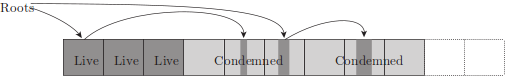
\includegraphics{figures/conc_2a}
    \caption
      {Αρχική διαμόρφωση αλγορίθμου Compressor. Όλες οι
       σελίδες ανήκουν στο χώρο-από.}
  \end{subfigure}

  \begin{subfigure}[b]{1.0\textwidth}
    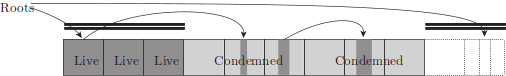
\includegraphics{figures/conc_2b}
    \caption
      {Υπολογισμός πληροφοριών προώθησης και προστασία όλων
       των σελίδων του χώρου-προς. Μεταξύ αυτών είναι οι
       δεσμευμένες σελίδες προς τις οποίες θα μεταφερθούν
       ζωντανά αντικείμενα και οι ζωντανές σελίδες που δεν
       έχουν καταδικασθεί για εκκένωση. Στη συνέχεια οι ρίζες
       των τροποποιητών δείχνουν προς το χώρο-προς. Τα νήματα
       τροποποιητές που θα προσπαθήσουν να προσπελάσουν μια
       προστατευμένη σελίδα του χώρου-προς θα παγιδευθούν.}
  \end{subfigure}
  
  \begin{subfigure}[b]{1.0\textwidth}
    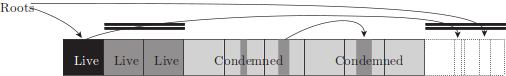
\includegraphics{figures/conc_2c}
    \caption
      {Η παγίδευση σε μία ζωντανή σελίδα προωθεί τους δείκτες
       που περιλαμβάνονται σε αυτή ώστε να αναφέρονται προς
       τα αντίγραφα στο χώρο-προς των προορισμών τους. Η προστασία
       της ζωντανής σελίδας αίρεται όταν έχουν πλέον προωθηθεί
       όλοι οι δείκτες αυτής.}
  \end{subfigure}
  
  \begin{subfigure}[b]{1.0\textwidth}
    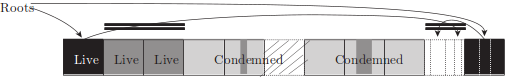
\includegraphics{figures/conc_2d}
    \caption
      {Η παγίδευση σε μία δεσμευμένη σελίδα του χώρου-προς
       γεμίζει τη σελίδα εκκενώνοντας σελίδες του χώρου-από.
       Τα πεδία δείκτες των αντικειμένων αυτών ενημερώνονται
       ώστε να δείχνουν προς το χώρο-προς. Στη συνέχεια αίρεται
       η προστασία της σελίδας του χώρου-προς και καταργείται
       η απεικόνιση προς πλήρως εκκενωμένες σελίδες του
       χώρου-από.}
  \end{subfigure}
  
  \begin{subfigure}[b]{1.0\textwidth}
    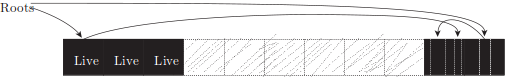
\includegraphics{figures/conc_2e}
    \caption
      {Η συμπύκνωση ολοκληρώνεται όταν όλες οι ζωντανές
       σελίδες έχουν σαρωθεί, όλοι οι δείκτες που αυτές
       περιλαμβάνουν έχουν προωθηθεί, όλα τα ζωντανά
       αντικείμενα καταδικασμένων σελίδων έχουν αντιγραφεί
       στο χώρο-προς και όλες οι αναφορές των τελευταίων
       έχουν προωθηθεί.}
  \end{subfigure}    
  \caption
    [Ταυτόχρονη εκτέλεση αλγορίθμου Compressor]
    {Ταυτόχρονη εκτέλεση αλγορίθμου Compressor.}
  \label{fig:conc_2}
\end{figure}

\section{Ταυτόχρονη Καταμέτρηση Αναφορών}
Εξετάσαμε τη συλλογή με καταμέτρηση αναφορών στο κεφάλαιο
~\ref{ch:refcnt}. Είδαμε πώς τα βασικά μειονεκτήματα της
απλοϊκής καταμέτρησης αναφορών αφορούν στην αδυναμία συλλογής
κύκλων σκουπιδιών και το υψηλό κόστος της διαχείρισης των
μετρητών αναφορών, ειδικά σε καταστάσεις συναγωνισμού μεταξύ
πολλαπλών νημάτων τροποποιητών. Ο αλγόριθμος Recycler (αλγόριθμος~\ref{alg:refcnt_5})
χρησιμοποιώντας την τεχνική της
δοκιμαστικής διαγραφής λύνει το πρόβλημα της αδυναμίας συλλογής
κύκλων σκουπιδιών. Η καταμέτρηση αναφορών με αναβολή αποτρέπει
τα νήματα τροποποιητές από το να μεταβάλλουν τους μετρητές
αναφορών τοπικών μεταβλητών, ενώ τέλος η καταμέτρηση αναφορών
με συγκέντρωση αποφεύγει τις περιττές ενημερώσεις των μετρητών
αναφοράς που ακυρώνονται από αργότερες λειτουργίες εγγραφής
δεικτών από τα νήματα τροποποιητές. Και οι τρεις λύσεις απαιτούν
την διακοπή του κόσμου την ώρα που ο συλλέκτης ενημερώνει τους
μετρητές αναφοράς και ανακτά τη μνήμη από αντικείμενα σκουπίδια. 
Εξετάζουμε τώρα πώς η απαίτηση για διακοπή του κόσμου μπορεί
να αποφευχθεί καθώς και ποιες αλλαγές απαιτούνται ώστε ένας
συλλέκτης με καταμέτρηση αναφορών να εκτελεστεί ταυτόχρονα με
τα νήματα τροποποιητές.

\subsection{Απλοϊκή καταμέτρηση αναφορών}
Η ορθότητα ενός συλλέκτη σκουπιδιών με καταμέτρηση αναφορών
απαιτεί την εξασφάλιση της ισχύος της αναλλοίωτης ότι ο μετρητής
αναφοράς κάθε αντικειμένου ισούται με το πλήθος των αναφορών
προς αυτό. Η εξασφάλιση της αναλλοίωτης είναι ιδιαίτερα περίπλοκη
όταν εμπλέκονται πολλαπλά νήματα τροποποιητές. Εκ πρώτης όψεως,
φαίνεται πώς η ασφαλής εκτέλεση της λειτουργίας \textenglish{\textproc{Write}}
είναι πιο δύσκολη από την ασφαλή εκτέλεση της λειτουργίας
\textenglish{\textproc{Write}}. Η ενημέρωση ενός δείκτη περιλαμβάνει τρεις
ενέργειες: την αύξηση του μετρητή αναφορών του νέου αντικειμένου
αναφοράς, τη μείωση του μετρητή αναφορών του παλαιού αντικειμένου
αναφοράς και την εγγραφή του δείκτη. Ο συντονισμός των ενεργειών
αυτών είναι απαραίτητος ούτως ώστε να αποφεύγεται η πρόωρη
αποδέσμευση αντικειμένων (λόγω για παράδειγμα προσωρινής μηδενικής
τιμής μετρητών αναφοράς) όσο και η επ' άπειρον αιώρηση σκουπιδιών
στο σωρό.

Η δυσκολία της ταυτόχρονης συλλογής σκουπιδιών με καταμέτρηση αναφορών δεν έγκειται μόνο στην
εξασφάλιση της ατομικής αύξησης και μείωσης μετρητών αναφορών. Το δυσκολότερο πρόβλημα αφορά
το συγχρονισμό των τροποποιήσεων των μετρητών αναφοράς με τις φορτώσεις και αποθηκεύσεις
δεικτών. Ένας τρόπος επίτευξης της ατομικότητας των λειτουργιών \textenglish{\textproc{Read}} και 
\textenglish{\textproc{Write}} του τροποποιητή είναι το κλείδωμα του αντικειμένου στο οποίο ανήκει το πεδίο
που διαβάζεται η γράφεται. 

Είναι επιθυμητή η εύρεση μιας λύσης που δε χρησιμοποιεί κλειδώματα αλλά πρωταρχικές εντολές
των οποίων η ατομικότητα εξασφαλίζεται από το υλικό. Δυστυχώς, οι πρωταρχικές 
εντολές που αφορούν μόνο μία θέση μνήμης δεν επαρκούν για την εξασφάλιση της ασφάλειας.
Ο Detlefs κ.ά. \cite{DBLP:conf/podc/DetlefsMMS01} [2001,2002b] δείχνουν πώς η λειτουργία \textenglish{\textproc{CompareAndSwap2}}, η οποία
ατομικά ενημερώνει δύο διαφορετικές θέσεις μνήμης επαρκεί. Παρότι δεν είναι αρκετή για τη διατήρηση
ακριβών τιμών των μετρητών αναφορών για κάθε χρονική στιγμή, η χρήση της εξασφαλίζει την ασθενέστερη
αναλλοίωτη πώς:
\begin{itemize}
\item όσο υπάρχει τουλάχιστον μια αναφορά προς ένα αντικείμενο, ο μετρητής αναφορών αυτού θα είναι
μη μηδενικός και
\item αν δεν υπάρχουν αναφορές προς ένα αντικείμενο, ο μετρητής αναφορών του τελικώς θα μηδενισθεί.
\end{itemize}

\subsection{Καταμέτρηση αναφορών με χρήση απομονωτή}
Οι αλγόριθμοι συλλογής σκουπιδιών με πρόθυμη καταμέτρηση
αναφορών απαιτούν τη χρήση είτε κλειδωμάτων είτε πρωταρχικών
ατομικών εντολών που τροποποιούν πολλές λέξεις μνήμης
ταυτόχρονα. Οι μηχανισμοί κλειδωμάτων δεν είναι ιδιαίτερα
φθηνοί, ενώ οι ατομικές πρωταρχικές εντολές πολλαπλών θέσεων
μνήμης δεν προσφέρονται από όλες τις αρχιτεκτονικές συνόλου
εντολών. Η καταμέτρηση αναφορών με αναβολή περιορίζει κάπως
το πρόβλημα με τη μη εφαρμογή λειτουργιών καταμέτρησης αναφορών
σε τοπικές μεταβλητές και την αναβολή της ανάκτησης μνήμης
αντικειμένων με μηδενικό μετρητή αναφορών. H
\textbf{καταμέτρηση αναφορών με χρήση απομονωτή} υποστηρίζει
την εκτέλεση πολυνηματικών εφαρμογών χρησιμοποιώντας απλές
εντολές φόρτωσης και αποθήκευσης στο φράγμα εγγραφής του
τροποποιητή.

Ο DeTreville \cite{detreville1990experience} σε έναν υβριδικό
συλλέκτη για τη γλώσσα Modula-2+ που χρησιμοποιεί έναν
εφεδρικό συλλέκτη με σήμανση και εκκαθάριση για την
αντιμετώπιση κύκλων σκουπιδιών, προκειμένου να αποφύγει το
κόστος του συγχρονισμού των λειτουργιών καταμέτρησης αναφορών
από διαφορετικά νήματα τροποποιητές, ανέθετε στα τελευταία
να καταχωρούν τις διευθύνσεις του παλαιού και του νέου
αντικειμένου αναφοράς ενός δείκτη σε έναν απομονωτή. Στη
συνέχεια, ένα ξεχωριστό νήμα καταμέτρησης αναφορών επεξεργάζεται
το χώρο καταχώρισης και προσαρμόζει τους μετρητές αναφορών
εξασφαλίζοντας με τον τρόπο αυτό την ατομικότητα των ενημερώσεων.
Δυστυχώς όμως η καταμέτρηση αναφορών με χρήση απομονωτή δεν
εξαφανίζει το πρόβλημα του συντονισμού των λειτουργιών
καταμέτρησης αναφορών και της εγγραφής του δείκτη. Ο
DeTreville πρότεινε δύο λύσεις, από τις οποίες όμως καμία δεν
είναι εξ ολοκλήρου ικανοποιητική. Η πρώτη του προσέγγιση αφορά
στην προστασία με κλείδωμα ολόκληρης της λειτουργίας
\textenglish{\textproc{Write}}. Για να αποφύγει το κόστος της ατομικής
εκτέλεσης κάθε λειτουργίας \textenglish{\textproc{Write}}, η δεύτερη λύση
του παρέχει σε κάθε νήμα τροποποιητή το δικό του τοπικό
απομονωτή, ο οποίος περιοδικά περνά στον έλεγχο του νήματος
καταμέτρησης αναφορών. Η προσέγγιση αυτή ωστόσο μεταφέρει
την ευθύνη της εξασφάλισης της ατομικής εκτέλεσης των
λειτουργιών \textenglish{\textproc{Write}} στον προγραμματιστή, ο οποίος
επιβαρύνεται με το ιδιαίτερα επίπονο έργο του χειρισμού
κλειδωμάτων.

Οι Bacon και Rajan \cite{DBLP:conf/ecoop/BaconR01} επίσης
παρέχουν σε κάθε νήμα τροποποιητή το δικό του τοπικό
απομονωτή, απαιτούν όμως η ενημέρωση ενός δείκτη να είναι
ατομική. Το φράγμα εγγραφής του τροποποιητή σε έναν επεξεργαστή
προσθέτει την παλαιά και την καινούρια τιμή του πεδίου $i$ ενός
αντικειμένου στον τοπικό απομονωτή $localUpdates$. Η καταμέτρηση
αναφορών των τοπικών μεταβλητών αναβάλλεται και πάλι, ενώ για
να αποτραπεί η πρόωρη διαγραφή αντικειμένων, ο χρόνος διαιρείται
σε \textbf{εποχές} χρησιμοποιώντας έναν καθολικό αριθμό εποχής
και τοπικούς αριθμούς εποχής για κάθε νήμα τροποποιητή.
Περιοδικά, όπως και στην καταμέτρηση αναφορών με αναβολή,
ένας επεξεργαστής θα διακόψει την εκτέλεση ενός νήματος
τροποποιητή και θα εξετάσει όλες τις τοπικές στοίβες,
καταχωρώντας τις αναφορές που βρίσκει σε έναν τοπικό απομονωτή
$myStackBuffer$. Στη συνέχεια ο επεξεργαστής μεταφέρει τους
απομονωτές $myStackBuffer$ και $myUpdates$ στο συλλέκτη και
ενημερώνει τον τοπικό αριθμό εποχής $e$. Τέλος, δρομολογεί
το νήμα συλλέκτη στον επόμενο επεξεργαστή πριν επαναφέρει
σε λειτουργία το σταματημένο νήμα τροποποιητή.

Το νήμα συλλέκτης εκτελείται στον επόμενο επεξεργαστή. Σε
κάθε κύκλο συλλογής $k$, ο συλλέκτης εφαρμόζει τις αυξήσεις
μετρητών αναφοράς της εποχής $k$ και τις μειώσεις μετρητών
αναφοράς της εποχής $k-1$. Τέλος, ενημερώνει τον καθολικό
αριθμό εποχής. Το πλεονέκτημα της μεθόδου είναι πώς ποτέ
δεν απαιτείται η αναστολή λειτουργίας όλων των νημάτων
τροποποιητών: ο συλλέκτης λειτουργεί εν-τη-πτήσει.

\begin{algorithm}
  \caption{Ταυτόχρονη καταμέτρηση αναφορών με χρήση απομονωτή}
  \label{alg:conc_7}
  \begin{algorithmic}[1]
    \State \textbf{shared} $epoch$
    \State \textbf{shared} $updatesBuffer[]$ \Comment{one buffer per epoch}
    \Statex
    \Procedure{Write}{$src$, $i$, $ref$}
      \If{$src=Roots$}
        \State $src[i] \gets ref$
      \Else
        \State $old \gets$ \Call{AtomicExchange}{$\&src[i]$, $ref$}
        \State \Call{log}{$old$, $ref$}
      \EndIf
    \EndProcedure
    \Statex
    \Procedure{log}{$old$, $new$}
      \State $myUpdates \gets myUpdates + [<old, new>]$
    \EndProcedure
    \Statex
    \Procedure{collect}{\null}
      \State $myStackBuffer \gets []$
      \ForAll{\textbf{local} $ref \; \textbf{in} \; myStacks$} \Comment{deferred reference counting}
        \State $myStackBuffer \gets myStackBuffer + [<ref, ref>]$
        \State \textbf{atomic}
        \State $updatesBuffer[e] \gets updatesBuffer[e] + myStackBuffer$
        \State \textbf{atomic}
        \State $updatesBuffer[e] \gets updatesBuffer[e] + myUpdates$
      \EndFor
        \State $myUpdates \gets []$
        \State $e \gets e + 1$
        \Statex
        \State $me \gets myProcessorId$
        \If{$me < MAX\_PROCESSORS$}
          \State \Call{schedule}{$collect$, $me+1$} \Comment{schedule collect() on the next processor}
        \Else \Comment{the last processor updates the reference counts}
          \ForAll{$<old, new> \; \textbf{in} \; updatesBuffer[epoch]$}
            \State \Call{addReference}{$old$}
          \EndFor
          \ForAll{$<old, new> \; \textbf{in} \; updatesBuffer[epoch]$}
            \State \Call{addReference}{$old$}
          \EndFor
          \State \Call{release}{$updatesBuffer[epoch-1]$} \Comment{free the old buffer}
          \State $epoch \gets epoch+1$
        \EndIf
    \EndProcedure
  \end{algorithmic}
\end{algorithm}

\subsection{Ταυτόχρονη κυκλική καταμέτρηση αναφορών}
Ο αλγόριθμος Recycler
\cite{DBLP:conf/pldi/BaconALRS01, DBLP:conf/ecoop/BaconR01}
ανακτά τη μνήμη από κύκλους σκουπιδιών εξερευνώντας υποψήφιους
υπογράφους και εφαρμόζοντας δοκιμαστική διαγραφή στους μετρητές
αναφορών. Παρότι η χρήση απομονωτή επιτυχώς μεταβιβάζει την
καταμέτρηση αναφορών σε έναν εφεδρικό επεξεργαστή, ο αλγόριθμος
Recycler αντιμετωπίζει τρία προβλήματα στην προσπάθεια συλλογής
κύκλων σκουπιδιών σε ένα περιβάλλον ταυτοχρονισμού:

\begin{enumerate}
\item Δεν μπορεί να εγγυηθεί πώς θα εξερευνήσει εκ νέου τον
  ίδιο υπογράφο καθώς ο γράφος μπορεί να έχει τροποποιηθεί
  από τα νήματα τροποποιητές ενόσω αυτός εντοπίζει κύκλους
  σκουπιδιών.
\item Διαγραφές δεικτών ενδέχεται να αποσυνδέσουν το γράφο.
\item Οι μετρητές αναφορών μπορεί να είναι ανενημέρωτοι.
\end{enumerate}

Η ασύγχρονη έκδοση του αλγορίθμου λειτουργεί σε δύο φάσεις
για να επιλύσει τα παραπάνω προβλήματα. Η πρώτη φάση είναι
λίγο πολύ η σύγχρονη εκδοχή του αλγορίθμου που παρουσιάσθηκε
στο κεφάλαιο \ref{ch:refcnt}. Ωστόσο ο ασύγχρονος Recycler
αναβάλλει την αποδέσμευση της μνήμης αντικειμένων που
εντοπίζει η διαδικασία \textenglish{\textproc{collectWhite}} (βλέπε
\ref{alg:refcnt_5}) μέχρι την επόμενη φάση, η οποία ελέγχει
ότι αυτά είναι ακόμη σκουπίδια. Η προσέγγιση αυτή παρουσιάζει
τα ακόλουθα μειονεκτήματα. Θεωρητικά και σπάνια στην πράξη
είναι πιθανόν ορισμένοι κύκλοι σκουπιδιών να μη συλλεγούν:
δεν υπάρχει εγγύηση πληρότητας του ασύγχρονου συλλέκτη.
Επιπλέον, η δοκιμαστική διαγραφή δε μπορεί να χρησιμοποιήσει
τον αυθεντικό μετρητή αναφορών αλλά έναν ειδικό κυκλικό
μετρητή αναφορών που επίσης αποθηκεύεται στην επικεφαλίδα
των αντικειμένων. Τρίτον, ο αλγόριθμος πρέπει να εξερευνήσει
εκ νέου τους υποψήφιους κύκλους σκουπιδιών στη δεύτερη φάση,
για να αποφύγει τη λανθασμένη αποδέσμευση ανακύκλωση ζωντανών
αντικειμένων.

Το βασικό πρόβλημα είναι πώς ο συλλέκτης Recycler προσπαθεί
να εφαρμόσει έναν αλγόριθμο που έχει σχεδιασθεί για σύγχρονη
συλλογή σε έναν ταυτόχρονο κόσμο όπου η τοπολογία του γράφου
αντικειμένων διαρκώς μεταβάλλεται.

\begin{figure}
  \centering
  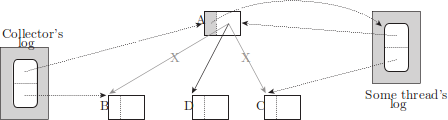
\includegraphics{figures/conc_4}
  \caption
    [Ταυτόχρονη καταμέτρηση αναφορών με συγκέντρωση.]
    {Ταυτόχρονη καταμέτρηση αναφορών με συγκέντρωση. Στη
     διάρκεια της προηγούμενης εποχής το αντικείμενο $A$
     τροποποιήθηκε ώστε να δείχνει στο αντικείμενο $C$
     και οι τιμές των πεδίων του αποθηκεύθηκαν σε κάποιον
     τοπικό απομονωτή καταγραφής. Ωστόσο, το αντικείμενο
     $A$ έχει τροποποιηθεί ξανά σε αυτήν την εποχή (δείχνει
     πλέον στο αντικείμενο $D$) και συνεπώς έχει σημανθεί
     ως βρώμικο και καταγραφεί ξανά. Το αρχικό αντικείμενο
     αναφοράς $B$ μπορεί να βρεθεί στον καθολικό χώρο
     καταγραφής, όπως και στο σχήμα~\ref{fig:refcnt_2}. Η
     αναφορά προς το αντικείμενο $C$ μπορεί να βρεθεί στον
     τοπικό απομονωτή καταγραφής ενός νήματος τροποποιητή,
     προς τον οποίο υπάρχει δείκτης από το αντικείμενο
     $A$.} 
\end{figure}

\subsection{Λήψη ενός στιγμιοτύπου του σωρού}
Στο κεφάλαιο~\ref{ch:refcnt} είδαμε πώς η καταμέτρηση
αναφορών με συγκέντρωση παρέχει στο συλλέκτη ένα στιγμιότυπο
του σωρού. Σε έναν τοπικό σε κάθε νήμα τροποποιητή απομονωτή,
ο οποίος μεταφέρεται σύγχρονα στο συλλέκτη, αποθηκεύονται
αντίγραφα αντικειμένων των οποίων πεδία δείκτες έχουν
τροποποιηθεί. Η λειτουργία όλων των νημάτων τροποποιητών
αναστέλλεται στην αρχή ενός κύκλου συλλογής, οι απομονωτές
διαβιβάζονται στο συλλέκτη και δεσμεύεται μνήμη για νέους
απομονωτές. Ο συλλέκτης απλώς χρησιμοποιεί το αντίγραφο ενός
αντικειμένου για να βρει τα παλαιά αντικείμενα αναφοράς των
δεικτών αυτού και να μειώσει τους μετρητές αναφορών αυτών,
ενώ χρησιμοποιεί την τρέχουσα κατάσταση του αντικειμένου για
να αυξήσει τους μετρητές αναφορών των νέων αντικειμένων
αναφορών των δεικτών αυτού. 

Το νήμα καταμέτρησης αναφορών μπορεί να εκτελείται ταυτόχρονα
με τα νήματα τροποποιητές. Στην περίπτωση αυτή, η εκτέλεση
των νημάτων τροποποιητών αναστέλλεται προσωρινά, μέχρις ότου
οι απομονωτές αυτών μεταβιβασθούν στο συλλέκτη. Μόλις
ολοκληρωθεί η μεταφορά, επανεκκινείται η εκτέλεση των νημάτων
τροποποιητών. Ο συλλέκτης είναι επιφορτισμένος με τη διόρθωση
των μετρητών αναφοράς των παλαιών και των νέων παιδιών κάθε
τροποποιημένου αντικειμένου. Η μείωση των μετρητών αναφοράς των
παλαιών παιδιών γίνεται εύκολα, όπως και πριν χρησιμοποιώντας
το αντίγραφο ενός αντικειμένου. Η αύξηση όμως των μετρητών
αναφοράς των παιδιών ενός αντικειμένου τη στιγμή μεταφοράς των
απομονωτών είναι πιο περίπλοκη, καθώς το αντικείμενο ενδέχεται
να έχει τροποποιηθεί εκ νέου.

Αν το αντικείμενο παραμένει καθαρό, τότε η κατάσταση του δεν
έχει αλλάξει και οι μετρητές αναφορών των τρεχόντων παιδιών
του αυξάνονται. Αν πάλι το αντικείμενο έχει τροποποιηθεί από
τη στιγμή μεταφοράς των απομονωτών, τότε έχει ξανασημανθεί ως
βρώμικο και η κατάσταση του τη στιγμή της μεταφοράς μπορεί να
βρεθεί σε ένα φρέσκο (καινούριο) απομονωτή κάποιου νήματος
τροποποιητή. Ο βρώμικος δείκτης του αντικειμένου αναφέρεται
σε αυτόν τον απομονωτή καταχώρισης, ο οποίος μπορεί να
αναγνωσθεί χωρίς να απαιτείται ο συγχρονισμός του συλλέκτη
με το νήμα στο οποίο ο τελευταίος ανήκει.

\subsection{Καταμέτρηση αναφορών με ολισθαίνουσες όψεις}
Για τη λήψη ενός στιγμιοτύπου του σωρού, αναστέλλεται η
εκτέλεση όλων των νημάτων τροποποιητών ταυτόχρονα προκειμένου
να πραγματοποιηθεί η μεταφορά των απομονωτών. Η τεχνική των
\textbf{ολισθαινουσών όψεων} χαλαρώνει τον παραπάνω περιορισμό
και προσφέρει τη δυνατότητα να διακόπτεται η εκτέλεση ενός
μόνο νήματος κάθε φορά. Είναι προφανές πώς αυτή η προσέγγιση
έχει ως αποτέλεσμα να παρέχεται στο συλλέκτη μια παραμορφωμένη
εικόνα του σωρού. Οι τιμές διαφορετικών αντικειμένων
καταγράφονται και μεταβιβάζονται στο νήμα συλλέκτη σε
διαφορετικές χρονικές στιγμές. Η τεχνική δεν απαιτεί τη χρήση
κλειδωμάτων ούτε και ατομικών πρωταρχικών λειτουργιών υλικού,
αλλά συντονίζει κάθε νήμα τροποποιητή με το νήμα συλλέκτη με
τη χρήση 4 χειραψιών όμοιων με εκείνες που χρησιμοποιούν οι
Doligez και Gonthier \cite{DBLP:conf/popl/DoligezG94}. Η
τεχνική των ολισθαινουσών όψεων χρησιμοποιείται ευρέως για
απλή, καθαρή καταμέτρηση αναφορών από τους Levanoni και
Petrank \cite{levanoni1999scalable, DBLP:conf/oopsla/LevanoniP01,
DBLP:journals/toplas/LevanoniP06}, για τη διαχείριση της
παλαιάς γενεάς γενεαλογικών συλλεκτών από τους Azatchi και
Petrank, \cite{DBLP:conf/oopsla/AzatchiLPP03}) καθώς και
σε συνδυασμό με κυκλική καταμέτρηση αναφορών από τον Paz
κ.ά. \cite{DBLP:conf/cc/PazPBKR05, DBLP:conf/cc/PazP07}.

\section{Θέματα προς εξέταση}
\subsection{Ταυτόχρονη σήμανση και εκκαθάριση}
Πολλά από τα ζητήματα που αφορούν την ταυτόχρονη συλλογή
σκουπιδιών με σήμανση και εκκαθάριση είναι κοινά για τους
περισσότερους ταυτόχρονους συλλέκτες. Η σχεδίαση ενός
ταυτόχρονου συλλέκτη είναι σαφώς πιο πολύπλοκη από τη
σχεδίαση ενός συλλέκτη που λειτουργεί με παύση του κόσμου.
Προκύπτει το ερώτημα κατά πόσον οι απαιτήσεις από το συλλέκτη
δικαιολογούν αυτήν την επιπλέον πολυπλοκότητα, καθώς μια
απλούστερη λύση, όπως η χρήση ενός γενεαλογικού συλλέκτη
να είναι αρκετή.

Οι γενεαλογικοί συλλέκτες σκουπιδιών προσφέρουν αναμενόμενους
χρόνους παύσης της τάξης των χιλιοστών του δευτερολέπτου για
τις περισσότερες εφαρμογές. Ωστόσο στη χειρότερη περίπτωση,
όπου και πρέπει να συλλεγεί ολόκληρος ο σωρός ο χρόνος παύσης
μιας εφαρμογής μπορεί να αυξηθεί υπερβολικά ανάλογα με το
μέγεθος του σωρού, τον όγκο των ζωντανών αντικειμένων κ.ο.κ.
Οι ταυτόχρονοι συλλέκτες από την άλλη πλευρά προσφέρουν
συντομότερους και πιο προβλέψιμους χρόνους παύσης.

Η ταυτόχρονη συλλογή με σήμανση και εκκαθάριση μπορεί όπως
και η μη ταυτόχρονη συλλογή με σήμανση και εκκαθάριση να
οδηγήσει σε κατακερματισμό του σωρού. Η συλλογή με αντιγραφή
και η συλλογή με σήμανση και συμπύκνωση εκτός από το ότι
αντιμετωπίζουν τον κατακερματισμό της μνήμης επιτρέπουν
επίσης την σειριακή εκχώρηση μνήμης, η οποία μπορεί να
είναι ταχύτερη από την εκχώρηση με χρήση ελεύθερης λίστας
και μπορεί επίσης να παρέχει καλύτερη τοπικότητα αναφορών
στα νήματα τροποποιητές. Από την άλλη πλευρά βέβαια οι συλλέκτες
σήμανσης και εκκαθάρισης χρησιμοποιούν αποδοτικότερα το
διαθέσιμο χώρο μνήμης σε σύγκριση με τους συλλέκτες αντιγραφής
καθώς δεν απαιτούν την ύπαρξη ενός εφεδρικού χώρου αντιγραφής.
Επιπλέον, οι μη μετακινούντες ταυτόχρονοι συλλέκτες έχουν
το εξής πλεονέκτημα σε σχέση με τους μετακινούντες ταυτόχρονους
συλλέκτες: η εξασφάλιση της συνέπειας του σωρού είναι σχετικά
απλή. Όλοι οι ταυτόχρονοι συλλέκτες απαιτούν από τα νήματα
τροποποιητές να τους ενημερώνουν σχετικά με τη μεταβολή της
τοπολογίας του σωρού ούτως ώστε να αποτραπεί η περίπτωση κάποιο
νήμα τροποποιητής να κρύβει αντικείμενα από το συλλέκτη. Ωστόσο,
οι ταυτόχρονοι μετακινούντες συλλέκτες πρέπει επιπλέον να
εξασφαλίσουν τόσο πώς μόνο ένα νήμα συλλέκτης μετακινεί ένα
αντικείμενο όσο και πώς η ενημέρωση όλων των δεικτών προς
ένα μετακινηθέν αντικείμενο εμφανίζεται να πραγματοποιείται
ατομικά στα νήματα τροποποιητές.

Τέλος η ταυτόχρονη συλλογή με σήμανση και εκκαθάριση προσφέρει
έναν αριθμό από σχεδιαστικές επιλογές υλοποίησης. Τα καινούρια
αντικείμενα μπορούν να εκχωρούνται είτε ως μαύρα, γκρι ή λευκά.
Ένα νέο αντικείμενο εκχωρείται πάντοτε ως μαύρο σε ένα μαύρο
τροποποιητή, ενώ ένας γκρι τροποποιητής προσφέρει περισσότερες
επιλογές. Τα νέα αντικείμενα μπορούν να εκχωρούνται ως μαύρα,
γκρι, ή λευκά και επιπλέον η απόφαση μπορεί να διαφέρει ανάλογα
με τη φάση του κύκλου συλλογής, τις αρχικές τιμές των πεδίων
του καινούριου αντικειμένου ή την πρόοδο της φάσης της εκκαθάρισης.

\subsection{Ταυτόχρονη αντιγραφή και συμπύκνωση}
Η ταυτόχρονη συλλογή αντιγραφής και σήμανσης και συμπύκνωσης
μειώνει τον κατακερματισμό της μνήμης και επίσης αποτρέπει
την εμφάνιση μεγάλων χρόνων παύσης. Όπως και στις άλλες
τεχνικές ταυτόχρονης συλλογής σκουπιδιών, ο συλλέκτης πρέπει να προστατεύεται
από τις ενέργειες του τροποποιητή ώστε να μην υπάρχουν
μη ορατά στο συλλέκτη προσβάσιμα αντικείμενα. Όμως επειδή
ο συλλέκτης μετακινεί αντικείμενα πρέπει και ο τροποποιητής
να προστατευθεί από τις ενέργειες του συλλέκτη ώστε να μην
προσπελάσει μη έγκυρα αντίγραφα αντικειμένων. Ο Baker
\cite{DBLP:journals/cacm/Baker78} προστατεύει τον τροποποιητή
εξασφαλίζοντας την διατήρηση μιας αναλλοίωτης του χώρου-προς
η οποία δεν επιτρέπει στον τροποποιητή τη διατήρηση δεικτών
προς αντικείμενα του χώρου-από. Ο Brooks \cite{DBLP:conf/lfp/Brooks84}
προστατεύει τον τροποποιητή επιτρέποντας του να συνεχίζει
να λειτουργεί στο χώρο-από και αναθέτοντάς του την ενημέρωση
των διευθύνσεων προώθησης προς αντικείμενα του χώρου-προς
καθώς αυτά δημιουργούνται. 
Η συμπύκνωση μπορεί να πραγματοποιηθεί με παρόμοιους τρόπους
χωρίς την απαίτηση να αντιγράφονται όλα τα αντικείμενα σε
έναν κύκλο συλλογής.

Η εφαρμογή μιας εκ των των παραπάνω τεχνικών πάντως μπορεί να
έχει ως αποτέλεσμα μεγαλύτερους χρόνους παύσης σε σύγκριση
με μη μετακινούντες ταυτόχρονους συλλέκτες: σε οποιαδήποτε
προσπάθεια προσπέλασης του σωρού ο τροποποιητής μπορεί να
παγιδευθεί και χρειασθεί να περιμένει μέχρις ότου ένα ή
περισσότερα αντικείμενα μετακινηθούν.

\subsection{Ταυτόχρονη καταμέτρηση αναφορών}
Το βασικό πρόβλημα της καταμέτρησης αναφορών σχετίζεται με το
πώς θα εξασφαλισθεί πώς οι μετρητές αναφορών των αντικειμένων
έχουν σωστές τιμές ενώ ο γράφος αντικειμένων τροποποιείται
ταυτόχρονα. Η απλούστερη λύση είναι να απαιτείται από τα νήματα
τροποποιητές να κλειδώνουν ένα αντικείμενο πριν το τροποποιήσουν.
Συνήθως όμως το κόστος των κλειδωμάτων θεωρείται υψηλό και συνεπώς
πρέπει να βρεθούν εναλλακτικές προσεγγίσεις. Οι τρέχουσες λύσεις
βασίζονται στην αποφυγή των καταστάσεων συναγωνισμού μεταξύ
νημάτων τροποποιητών που μπορεί να διακινδυνεύσουν την συνέπεια
των μετρητών αναφορών. Ο διαχειριστής μνήμης ενδιαφέρεται μόνο
να εξασφαλίσει τη συνέπεια του σωρού: δεν είναι δική του ευθύνη
η εξασφάλιση της ορθότητας του προγράμματος χρήστη.

Για να διατηρηθεί η συνοχή του σωρού, απαιτείται η σειριοποίηση
των εγγραφών δεικτών και των λειτουργιών ενημέρωσης των μετρητών
αναφορών. Μια μερική λύση είναι η χρήση της καταμέτρησης αναφορών
με αναβολή, καθώς έτσι αναβάλλεται η αποδέσμευση της μνήμης των 
σκουπιδιών η οποία μάλιστα ανατίθεται σε ένα ξεχωριστό νήμα
συλλέκτη. Ωστόσο η λύση αυτή αφορά μόνο τις φορτώσεις και
αποθηκεύσεις δεικτών και όχι τις εγγραφές σε πεδία δείκτες στο
εσωτερικό αντικειμένων. Προκύπτει έτσι το ερώτημα του πώς μπορούν
οι ενημερώσεις μετρητών αναφοράς που απορρέουν από τις εγγραφές
πεδίων δεικτών να ανατεθούν από τα νήματα τροποποιητές σε ένα
νήμα συλλέκτη. Η απλούστερη λύση είναι κάθε νήμα τροποποιητής
να απομονώνει τις λειτουργίες καταμέτρησης αναφορών του και να
τις περνά περιοδικά στο νήμα συλλέκτη. Η καταμέτρηση αναφορών
με συγκέντρωση πηγαίνει την παραπάνω ιδέα ένα βήμα πιο πέρα:
λαμβάνοντας ένα στιγμιότυπο των αντικειμένων πριν αυτά τροποποιηθούν
επιτρέπει στο νήμα συλλέκτη να αποφύγει την εφαρμογή περιττών
ενημερώσεων των μετρητών αναφορών. Και στις δύο περιπτώσεις
πάντως η διαχείριση των μετρητών αναφορών και η αποδέσμευση
αντικειμένων διαχωρίζεται πλήρως από τις εγγραφές δεικτών
και πραγματοποιείται εξ' ολοκλήρου από ένα ξεχωριστό νήμα
συλλέκτη ή και πολλαπλά νήματα συλλέκτες που τρέχουν παράλληλα.
Η λήψη ενός στιγμιοτύπου της κατάστασης του σωρού επίσης
απλοποιεί την κυκλική καταμέτρηση αναφορών. Οι αλγόριθμοι
δοκιμαστικής διαγραφής πρέπει να διασχίσουν έναν υπογράφο του
σωρού πολλές φορές. Διασχίζοντας το στιγμιότυπο, ο συλλέκτης
μπορεί να εξασφαλίσει πώς εξερευνά τον ίδιο υπογράφο κάθε
φορά παρά τις ταυτόχρονες δραστηριότητες νημάτων τροποποιητών.

\end{greek}

\begin{greek}
\chapter{Συλλογή σκουπιδιών πραγματικού χρόνου}\label{ch:rt}
Οι ταυτόχρονοι και αυξητικοί αλγόριθμοι συλλογής σκουπιδιών
που εξετάσαμε στο προηγούμενο κεφάλαιο προσπαθούν να μειώσουν
τους χρόνους παύσης που αντιλαμβάνεται ο τροποποιητής, είτε
με σπάσιμο του κύκλου συλλογής σε μικρά κβάντα χρόνου και την
παρεμβολή της εκτέλεσης του συλλέκτη στην εκτέλεση του τροποποιητή
για κάθε ένα από αυτά στον ίδιο επεξεργαστή, είτε με την ταυτόχρονη
εκτέλεση του συλλέκτη σε έναν διαφορετικό επεξεργαστή. Πολλοί
από τους αλγορίθμους αυτούς σχεδιάσθηκαν με στόχο την υποστήριξη
εφαρμογών πραγματικού χρόνου όπου οι παύσεις μεγάλης διάρκειας
έχουν ως αποτέλεσμα τη δραματική μείωση της επίδοσης. Παρότι
οι αρχικοί αυξητικοί και ταυτόχρονοι συλλέκτες κατηγοριοποιήθηκαν
ως πραγματικού χρόνου, αυτό είναι αληθές μόνο εάν τηρούνται
κάποιες αυστηρές προϋποθέσεις. Ωστόσο, όπως αντιλαμβανόμαστε
σήμερα τα συστήματα πραγματικού χρόνου, κανείς από τους αλγορίθμους
αυτούς δεν μπορεί να παρέχει ισχυρές εγγυήσεις προόδου στον
τροποποιητή. Η πρόοδος του τροποποιητή δεν μπορεί πλέον να
εγγυηθεί όταν ο τελευταίος πρέπει να αποκτήσει κάποιο κλείδωμα
(κατά την εκτέλεση κάποιου φράγματος εγγραφής ή ανάγνωσης για
παράδειγμα). Ακόμη χειρότερα, ένας διακοπτός αλγόριθμος χρονοδρομολόγησης
ενδέχεται τυχαία να δίνει μεγαλύτερη προτεραιότητα στη δρομολόγηση
των ταυτόχρονων νημάτων συλλεκτών. Η \textbf{συλλογή σκουπιδιών
πραγματικού χρόνου RTGC)} οφείλει να δικαιολογεί με ακρίβεια
τις παύσεις λειτουργίας των νημάτων τροποιητών, ενώ ταυτόχρονα
εξασφαλίζει τη μη υπέρβαση των χωρικών ορίων.

\section{Συστήματα πραγματικού χρόνου}
Τα \textbf{συστήματα πραγματικού χρόνου} επιβάλλουν λειτουργικές
προθεσμίες σε συγκεκριμένες εργασίες μιας εφαρμογής. Αυτά τα
συστήματα πραγματικού χρόνου θα πρέπει να αποκρίνονται σε
γεγονότα εισόδου εντός ενός καθορισμένου χρονικού παραθύρου.
Μια εργασία που αποτυχγάνει στην τήρηρη μιας προθεσμίας μπορεί
να υποβαθμίσει την υπηρεσία ή ακόμη χειρότερα να προκαλέσει
την πλήρη κατάρρευση του συστήματος. Συνεπώς, ένα σύστημα
πραγματικού χρόνου οφείλει να είναι ορθό όχι μόνο όσον αφορά
τη λογική της εφαρμογής, αλλά και όσον αφορά την αποκρισιμότητα
της σε γεγονότα πραγματικού χρόνου.

Ένα \textbf{απαλό σύστημα πραγματικού χρόνου} (όπως για παράδειγμα
η απεικόνιση βίντεο) μπορεί να ανεχτεί χαμένες προσθεσμίες εις
βάρος της ποιότητας της υπηρεσίας. Ενώ πολλές χαμένες προθεσμίες
θα έχουν ως αποτέλεσμα μη αποδεκτή ποιότητα υπηρεσίας, μια
συνηθισμένη χαμένη προθεσμία δεν την επηρεάζει πολύ. Ο Printezis
\cite{DBLP:journals/scp/Printezis06} προτείνει ένα απαλό στόχο
που προσδιορίζει ταυτόχρονα ένα μέγιστο χρόνο συλλογής, μία χρονική
σχισμή συγκεκριμένης διάρκειας και έναν αποδεκτό ρυθμό αποτυχίας.
Σε κάθε διάστημα εντός αυτής της χρονικής σχισμής, ο συλλέκτης
πρέπει να αποφύγει να χρησιμοποιήσει περισσότερο χρόνο από το
μέγιστο και όλες οι παραβιάσεις αυτού του στόχου πρέπει να είναι
εντός του αποδεκτού ρυθμού αποτυχίας. 

Ένας τέτοιος απαλός στόχος είναι ανεπαρκής για \textbf{σκληρά
συστήματα πραγματικού χρόνου} (όπως για παράδειγμα ο έλεγχος
ενός κινητήρα), όπου οι χαμένες προθεσμίες σημαίνουν την αποτυχία
του συστήματος. Ένα ορθώς σχεδιασμένο σκληρό σύστημα πραγματικού
χρόνου οφείλει να εξασφαλίζει την ικανοποίηση όλων των περιορισμών
πραγματικού χρόνου. Λαμβάνοντας υπόψη την παρουσία τέτοιων χρονικών
περιορισμών, είναι σημαντικό η αποκρισιμότητα της συλλογής
σκουπιδιών σε συστήματα πραγματικού χρόνου να μπορεί να χαρακτηρισθεί
με τέτοιο τρόπο ώστε να απεικονίζει τόσο τις ανάγκες της εφαρμογής
όσο και τη συμπεριφορά του συλλέκτη.

Η συνολική επίδοση ή ρυθμαπόδοση των συστημάτων πραγματικού χρόνου
είναι λιγότερο σημαντική από την \textbf{προβλεψιμότητα} της
επίδοσης. Η χρονική συμπεριφορά μιας εργασίας πραγματικού χρόνου
θα πρέπει να μπορεί να προσδιορισθεί είτε αναλυτικά κατά τη
σχεδίαση είτε εμπειρικά κατά την εκτέλεση ούτως ώστε ο χρόνος
απόκρισης της να είναι γνωστός εξαρχής (σε κάποιο αποδεκτό
βαθμό εμπιστοσύνης). Ο \textbf{χρόνος εκτέλεσης χειρότερης περίπτωσης}
μιας εργασίας είναι ο μέγιστος χρόνος που μπορεί να χρειαστεί
(αγνοώντας τυχόν επαναδρομολόγηση) για την απομονωμένη εκτέλεση
της εργασίας σε μια συγκεκριμένη πλατφόρμα υλικού. Συστήματα πραγματικού
χρόνου που υποστηρίζουν την ταυτόχρονη εκτέλεση πολλών εργασιών
πρέπει να δρομολογούν τις εργασίες με γνώμονα την ικανοποίηση
των χρονικών περιορισμών των τελευταίων. Η γνώση σχετικά με
την ικανοποίηση αυτών των περιορισμών απαιτεί την εκ των
προτέρων πραγματοποίηση \textbf{ανάλυσης δρομολόγησης}, υποθέτοντας
ένα συγκεκριμένο αλγόριθμο χρονοδρομολόγησης (συνήθως βασισμένο
σε προτεραιότητες).

Οι εφαρμογές πραγματικού χρόνου συχνά τρέχουν σε εξειδικευμένα
ενσωματωμένα συστήματα. Οι αλγόριθμοι αυξητικής συλλογής
σκουπιδιών είναι κατάλληλοι για χρήση σε ενσωματωμένα συστήματα
με μονοπύρηνο επεξεργαστή, ενώ οι αλγόριθμοι παράλληλης και
ταυτόχρονης συλλογής σκουπιδιών είναι πιο κατάλληλοι για χρήση
σε ενσωματωμένα συστήματα με πολυπύρηνο επεξεργαστή. Σε κάθε
περίπτωση πάντως, τα ενσωματωμένα συστήματα συχνά επιβάλλουν
στενότερους χωρικούς περιορισμούς σε σύγκριση με τις πλατφόρμες
γενικού σκοπού.

Για όλους τους παραπάνω λόγους, οι αλγόριθμοι συλλογής με
παύση του κόσμου, παράλληλης συλλογής ή ακόμη και ταυτόχρονης
συλλογής που επιβάλλει όμως μη προβλέψιμους χρόνους παύσης
δεν είναι κατάλληλοι για χρήση σε εφαρμογές πραγματικού
χρόνου. Ας θεωρήσουμε για παράδειγμα τη δρομολόγηση συλλογής
του σχήματος~\ref{fig:rt_1}, η οποία προκύπτει όταν η προσπάθεια
ανάκτησης μνήμης εξαρτάται από το συνολικό πλήθος και μέγεθος
των αντικειμένων που χρησιμοποιεί η εφαρμογή, τις διασυνδέσεις
μεταξύ των αντικειμένων αυτών καθώς και το βαθμό δυσκολίας ανάκτησης
αρκετής μνήμης για την ικανοποίηση μελλοντικών αιτημάτων. Δοθείσης
μιας τέτοιας δρομολόγησης, ο τροποποιητής δεν έχει κάποια εγγύηση
προβλέψιμης και βιώσιμης χρήσιμοποίησης του επεξεργαστή.

\begin{figure}
  \centering
  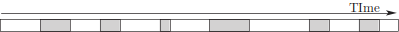
\includegraphics{figures/rt_1}
  \caption
    [Μη προβλέψιμη συχνότητα και διάρκεια εκτέλεσης συμβατικών
     συλλεκτών σκουπιδιών.]
    {Μη προβλέψιμη συχνότητα και διάρκεια εκτέλεσης συμβατικών
     συλλεκτών σκουπιδιών. Οι παύσεις λόγω συλλογής απεικονίζονται
     με γκρι χρώμα.}
  \label{fig:rt_1} 
\end{figure}

\section{Δρομολόγηση συλλογής πραγματικού χρόνου}
Ο χρόνος και ο τρόπος πυροδότησης της εκτέλεσης εργασιών συλλογής
σκουπιδιών είναι οι βασικοί παράγοντες που επηρεάζουν την επίδραση
του συλλέκτη στον τροποποιητή. Οι αλγόριθμοι συλλογής με παύση
του κόσμου αναβάλλουν όλες τις εργασίες συλλογής μέχρις ότου η
μη ικανοποίηση ενός αιτήματος εκχώρησης μνήμης εντοπίσει την
έλλειψη χώρου. Οι αλγόριθμοι αυξητικής συλλογής επιβαρύνουν
τις λειτουργίες εγγραφής και ανάγνωσης του τροποποιητή καθώς
και τις λειτουργίες εκχώρησης με ενέργειες συλλογής. Οι αλγόριθμοι
ταυτόχρονης συλλογής τέλος πυροδοτούν την εκτέλεση ενός μικρού
φορτίου συλλογής ταυτόχρονα (πιθανώς και παράλληλα) με την
εκτέλεση του τροποποιητή, χρησιμοποιώντας φράγματα τροποποίησης
για το συγχρονισμό του συλλέκτη με τον τελευταίο. Για να διατηρηθεί
μια κατανάλωση χώρου σταθερής κατάστασης, ο συλλέκτης πρέπει
να ελευθερώνει και ανακυκλώνει νεκρά αντικείμενα με τον ίδιο
ρυθμό που ο τροποποιητής δημιουργεί καινούρια αντικείμενα.
Πιθανός κατακερματισμός της μνήμης οδηγεί σε σπατάλη χώρου και
έχει ως αποτέλεσμα την αδυναμία ικανοποίησης αιτημάτων εκχώρησης
από τον εκχωρητή, εκτός και αν ο συλλέκτης συμπυκνώσει το
σωρό. Η μεταφορά αντικειμένων ωστόσο που προκαλεί η συμπύκνωση,
είναι ακριβή διαδικασία και μπορεί να επηρεάσει δυσμενώς την
προσπάθεια ικανοποίησης περιορισμών πραγματικού χρόνου.

Οι Henriksson \cite{henriksson1998scheduling}, Detlefs \cite{DBLP:conf/isorc/Detlefs04},
Cheng και Blelloch \cite{DBLP:conf/pldi/ChengB01} καθώς και
οι Pizlo και Vitek \cite{DBLP:conf/pldi/PizloPS08}, προτείνουν
εναλλακτικές τεχνικές για τη δρομολόγηση της συλλογής σκουπιδιών
σε συστήματα πραγματικού χρόνου, καθώς και για το χαρακτηρισμό
του πώς αυτή επηρεάζει την εκτέλεση του τροποποιητή.

Η \textbf{δρομολόγηση με βάση την εργασία} επιβάλλει έργο
συλλογής ως φόρο στις μονάδες εργασίας του τροποποιητή. Η
\textbf{δρομολόγηση με βάση την αδράνεια} τρέχει έργο συλλογής
στη διάρκεια των χρονικών διαστημάτων αδράνειας των νημάτων
τροποποιητών πραγματικού χρόνου.
Η \textbf{δρομολόγηση με βάση το χρόνο} δεσμεύει ένα προκαθορισμένο
διάστημα του χρόνου εκτέλεσης για την εκτέλεση του εργασιών
συλλογής, κατά τη διάρκεια του οποίου αναστέλλεται η εκτέλεση του
τροποποιητή.

\section{Περαιτέρω μελέτη}

\end{greek}

%\include{ch10}

%\appendix
%\chapter{Μεταφράσεις Ξένων Όρων}

%\begin{tabular}{l||l}
%\Large{\bfseries{Μετάφραση}} & \Large{\bfseries{Αγγλικός 'Ορος}}\\
%συστάδα & clump\\ 
%λεωφόρος & avenue
%\end{tabular}

% \backmatter
\cleardoublepage % start at the next odd page
\phantomsection % correct hyperlinking
\addcontentsline{toc}{chapter}{\bibname} % add bibliography section to toc

\bibliography{references}
\bibliographystyle{plain} % plain/abbrv/alpha/abstract/apalike/...

\end{document}
